\documentclass[12pt, a4paper,twoside]{book}


\usepackage[latin1]{inputenc}
\usepackage[spanish]{babel}
\usepackage{amsmath}
\usepackage{amsfonts}
\usepackage{amssymb}
\usepackage{makeidx}
\usepackage{graphicx}
\usepackage[left=2cm,right=2cm,top=2cm,bottom=2cm]{geometry}
\usepackage{float}
\usepackage{colortbl}	% Coloreado de columnas de tablas
\usepackage[cmyk]{xcolor}
\usepackage{multirow}
\usepackage{rotating}
\usepackage{longtable}
\usepackage{pdfpages}
\usepackage[latin1]{inputenc}
\usepackage{listings}

\usepackage{color}
\definecolor{gray}{rgb}{0.4,0.4,0.4}
\definecolor{darkblue}{rgb}{0.0,0.0,0.6}
\definecolor{cyan}{rgb}{0.0,0.6,0.6}

%\lstset{
%  basicstyle=\ttfamily,
%  columns=fullflexible,
%  showstringspaces=false,
%  commentstyle=\color{gray}\upshape
%}

\lstset{ %
language=Java,                % choose the language of the code
basicstyle=\footnotesize,       % the size of the fonts that are used for the code
numbers=left,                   % where to put the line-numbers
numberstyle=\footnotesize,      % the size of the fonts that are used for the line-numbers
stepnumber=1,                   % the step between two line-numbers. If it is 1 each line will be numbered
numbersep=5pt,                  % how far the line-numbers are from the code
backgroundcolor=\color{white},  % choose the background color. You must add \usepackage{color}
showspaces=false,               % show spaces adding particular underscores
showstringspaces=false,         % underline spaces within strings
showtabs=false,                 % show tabs within strings adding particular underscores
frame=single,           % adds a frame around the code
tabsize=2,          % sets default tabsize to 2 spaces
captionpos=b,           % sets the caption-position to bottom
breaklines=true,        % sets automatic line breaking
breakatwhitespace=false,    % sets if automatic breaks should only happen at whitespace
escapeinside={\%*}{*)}          % if you want to add a comment within your code
}

\lstdefinelanguage{XML}
{
  morestring=[b]",
  morestring=[s]{>}{<},
  morecomment=[s]{<?}{?>},
  stringstyle=\color{black},
  identifierstyle=\color{darkblue},
  keywordstyle=\color{cyan},
  morekeywords={xmlns,version,type}% list your attributes here
}

\author{Vanesa Gonz�lez P�rez}

\newcommand{\HRule}{\rule{\linewidth}{0.5mm}}
\renewcommand{\arraystretch}{1.5} % alto de la tabla


\newcommand{\Dflecha}{\mathop{\Rightarrow}\limits}
\newcommand{\ldflecha}{\mathop{\longrightarrow}\limits}


%CONTROLA LOS MARGENES DEL TEXTO
% margen {izquierda}{derecha}{arriba}{abajo}
\usepackage{anysize}
\marginsize{3cm}{3cm}{2.5cm}{2.5cm}

%\headheight = 11pt
%\topmargin=-0.68cm % Controla la altura
\headsep=0.7cm % margen de separación entre la cabecera y el texto

\setlength{\parindent}{7mm}%sangria la primera linea

%Para conseguir que en las páginas en blanco no ponga cabeceras
\makeatletter
\def\clearpage{%
  \ifvmode
    \ifnum \@dbltopnum =\m@ne
      \ifdim \pagetotal <\topskip
        \hbox{}
      \fi
    \fi
  \fi
  \newpage
  \thispagestyle{empty}
  \write\m@ne{}
  \vbox{}
  \penalty -\@Mi
}

%  FORMATO ENCABEZADO
%==========================================
\usepackage{fancyhdr}
\pagestyle{fancy}
\fancyhf{} %borra los ajustes del encabezado
\fancyhead[LO]{\leftmark} % En las páginas impares, parte izquierda del encabezado, aparecerá el nombre de capítulo
\fancyhead[RE]{\rightmark} % En las páginas pares, parte derecha del encabezado, aparecerá el nombre de sección
\fancyhead[RO,LE]{\thepage} % Números de página en las esquinas de los encabezados

%  NOTAS AL PIE DE PÁGINA
%==========================================

\footnotesep=0pt  %Separación de las líneas en las notas a pie de página
\newcommand{\newfootnote}[1]{\footnote{\hspace*{2mm}#1}}%Nueva nota de pie de página.
\renewcommand{\baselinestretch}{1}%Ancho de separación entre líneas dentro de un párrafo
\footskip = 30cm
\usepackage[marginal,flushmargin,norule]{footmisc} %paquete para controlar las notas de pie de página
\setlength\footnotemargin{1.8em} %Margen de la nota de pie de página
\setlength{\skip\footins}{8mm}%Separación entre el texto principal y las notas pie de pagina
\setlength{\parskip}{15pt}

%DEFINICIÓN DE ÓRDENES
\def\href#1#2{ #1 (#2)}
\def\url#1{#1}
\def\xmlsch{\textit{XML Schema }}
\def\xmlschf{\textit{XML Schema}}
\def\latex{\textit{Latex}}
\def\tex{\textit{Tex}}
\def\winedt{\textit{WinEdt}}

% Profundidad de la tabla de contenido.
\setcounter{tocdepth}{3} % nivel de sección y subsección, etc.
\setcounter{secnumdepth}{3}

% Se declaran las extensiones de los gr�ficos. Por defecto, .eps.
\DeclareGraphicsExtensions{.eps}

% Declaracion de colores
\definecolor{verdeOscuro}{rgb}{0,0.5,0}
\definecolor{naranjaOscuro}{rgb}{0.5,0.25,0}


\colorlet{verde-oscuro}{green!20!black}
\colorlet{verde-oscuro1}{green!50!green}
\colorlet{verde}{green!50!black}

\colorlet{marron-oscuro}{brown!20!black}
\colorlet{marron}{brown!50!black}

\colorlet{amarillo-claro}{yellow!50!white}

\colorlet{rosa}{red!50!white}



\begin{document}

\renewcommand{\listtablename}{�ndice de tablas}
\renewcommand{\tablename}{Tabla}

\begin{titlepage}

\begin{center}

\begin{tabular}[c]{ccc}
   
\includegraphics[width=2.2cm, height=2.7cm]{./img/logo_uco.jpg}
    % Esta siguiente linea coloca a cada imagen en una celda.
    \vspace*{0.6cm}\mbox{} & \hspace*{0.1cm}
    
    


\textsc{\LARGE \textbf{Universidad de C�rdoba}}



% 
\includegraphics[width=6.2cm, height=2.5cm]{./img/cordoba.jpg}
  \vspace*{0.6cm}\mbox{} & \hspace*{0.1cm}
    

\includegraphics[width=2.7cm, height=2.8cm]{./img/informatica.jpg}
 \end{tabular}\\[0.9cm]

% Upper part of the page

\textsc{\Large Escuela Polit�cnica Superior de C�rdoba}\\[1cm]
\textsc{\LARGE Ingenier�a Inform�tica}\\[1.5cm]


% Title
\HRule \\[0.4cm]
{ \Large \bfseries Proyecto de fin de carrera}\\[0.7cm]

{ \LARGE \bfseries SimAS: Simulador de An�lisis Sint�cticos}\\[0.4cm]

\HRule \\[1.3 cm]

\begin{center}
\textbf{\Large MANUAL DE USUARIO} \\[2 cm]
\end{center}


\begin{flushright}
{\Large \textbf{\emph{Autora}}\\[0.2cm]
\Large Vanesa Gonz�lez P�rez}\\[0.2cm]
\end{flushright}


\begin{flushright}
{\Large \textbf{\emph{Director}} \\[0.2cm]
\Large Dr.Nicol�s Luis Fern�ndez Garc�a}\\[2cm]
\end{flushright}


\vfill 

% Bottom of the page
{\LARGE C�rdoba, 9 de Junio de 2015}

\end{center}

\end{titlepage}



\vspace*{15cm}
\clearpage
\thispagestyle{empty}
\vspace*{2cm}


Dr. Nicol�s Luis Fern�ndez Garc��a, Profesor Titular de Universidad del �rea de Conocimiento de Ciencias de la Computaci�n e Inteligencia Artificial y adscrito al Departamento de Inform�tica y An�lisis Num�rico


\textbf{INFORMA}

Que el presente proyecto de fin de carrera, titulado ``SimAS: Simulador de An�lisis Sint�cticos'', ha sido realizado bajo por Vanesa Gonz�lez P�rez (Ingenier�a Inform�tica), reuniendo, a juicio, los requisitos exigidos a este tipo de trabajos.


Y para que cosnte donde proceda, firma el presente informe en C�rdoba a 9 de junio de 2015.

\vspace{3cm}

\centerline{Nicol�s Luis Fern�ndez Garc�a  \hspace{1cm} Vanesa Gonz�lez P�rez}


\frontmatter

\tableofcontents

\listoffigures

\listoftables


%%%%%%%%%%%%%%%%%%%%%%%%%%%%%%%
%%% COMENTADO POR NICOL�S LUIS
%%%\listofalgorithms
%%%%%%%%%%%%%%%%%%%%%%%%%%%%

\part{Introducci�n}

\mainmatter


\chapter {Introducci�n}

La aplicaci�n SimAS es una herramienta did�ctica, interactiva y multiplataforma que permite la adquisici�n de los fundamentos de los analizadores sint�cticos y trabajar con ellos.

Mediante el uso de esta aplicaci�n se puede aprender a crear gram�ticas de contexto libre y realizar simulaciones de los m�todos de an�lisis sint�ctico descendente as� como de los m�todos de an�lisis sint�ctico ascendente LR. Adem�s, SimAS le ayudar� a comprender mejor los fundamentos en los que se basan estos m�todos, convirti�ndose en un valioso aliado que le facilitar� el aprendizaje de esta materia.

A lo largo de este manual, cualquier estudiante de Ingenier�a Inform�tica con las nociones b�sicas sobre las gram�ticas de contexto libre y los an�lisis sint�cticos, aprender� a manejar eficazmente la aplicaci�n.

El contenido de este manual de usuario es el siguiente:


\begin{itemize}


  \item Instalaci�n y desinstalaci�n del programa.
  \item Caracter�sticas de la interfaz de SimAS.
  \item Editor de gram�ticas.
  \item Simulaci�n Descendente.
  \item Simulaci�n Ascendente.
  \item Ejemplos pr�cticos.

\end{itemize}



\chapter{Objetivos}

De acuerdo a la identificaci�n real y t�cnica del problema que se ha realizado en el cap�tulo anterior, a continuaci�n se expondr�n todos los objetivos funcionales que se pretenden alcanzar con el desarrollo de este proyecto.

\section{Objetivo principal}

El principal objetivo es el de construir una herramienta completa que facilite el aprendizaje del An�lisis  Sint�ctico tanto ascendente como descendente, de forma que permita a todas las personas interesadas en la materia aprender de una manera sencilla, r�pida y amena.

El software deber� permitir realizar las siguientes tareas principales:

\begin{enumerate}

\item Editor de gram�ticas de contexto libre.

\item An�lisis descendente y predictivo.

\item An�lisis ascendente:

\begin{itemize}

\item An�lisis SLR.

\item An�lisis LR-can�nico.

\item An�lisis LALR.

\end{itemize}

\item Detecci�n y recuperaci�n de errores.

\item Tutorial.

\item Ayuda.

\end{enumerate}

\section{Objetivos espec�ficos}

Adem�s de las tareas principales comentadas anteriormente, la aplicaci�n deber� cumplir los siguientes objetivos secundarios:

\begin{itemize}
  \item Editor de gram�ticas:
    \begin{itemize}
      \item Creaci�n de una gram�tica de contexto libre.
      \item Edici�n del vocabulario.
      \item Gesti�n de producciones.
      \item Validaci�n de la gram�tica.
      \item Carga y almacenamiento de la gram�tica.
      \item Generaci�n de informes.
    \end{itemize}
  \item Simulador descendente:
    \begin{itemize}
     \item Construcci�n de la tabla predictiva.
     \item Simulaci�n de la gram�tica.
     \item Gesti�n de errores.
     \item Generaci�n de informes.
    \end{itemize}
  \item Simulador ascendente:
  	\begin{itemize}
  	 \item Construcci�n de la tabla de an�lisis LR.
  	 \item Simulaci�n de los m�todos: SLR, LR-can�nico y LALR.
	 \item Gesti�n de errores.
	 \item Generaci�n de informes.  	 
  	\end{itemize}
  \item Tutorial
    \begin{itemize}
     \item Conceptos te�ricos del an�lisis sint�ctico.
     \item Ejemplos.
    \end{itemize}
  \item Ayuda.
    \begin{itemize}
     \item Instalaci�n y desinstalaci�n.
     \item Interfaz y modulos del programa.
     \item Resoluci�n de problemas.
    \end{itemize}

\end{itemize}









\chapter{Antecedentes}

En este cap�tulo se mostrar�n los antecedentes de este proyecto. En �l se tratar�n los siguientes temas:

\begin{itemize}
\item Los fundamentos te�ricos sobre los que se basa el proyecto, como son las gram�ticas formales, el an�lisis descendente y el an�lisis ascendente.
\item Descripci�n de los proyectos fin de carrera ya existentes, basados en el tema que estamos tratando.
\item Por �ltimo, se realizar� la justificaci�n del desarrollo del proyecto.
\end{itemize}



\section{Fundamentos te�ricos}

Como ya se ha mencionado en apartados anteriores, el objetivo del proyecto es el de realizar un simulador del An�lisis sint�ctico descendente y ascendente a partir de una gram�tica de contexto libre. 

A continuaci�n se lleva a cabo una introducci�n a ambos an�lisis sint�cticos, con el fin de que el lector se familiarice con el tema tratado en este proyecto.

\subsection{Gram�ticas formales}

Una gram�tica formal es un conjunto de reglas para reescribir cadenas de caracteres, junto con un s�mbolo inicial desde el cual debe comenzar la reescritura. Por lo tanto, una gram�tica formal generalmente se piensa como una generadora de lenguajes.

Un lenguaje formal es de contexto libre si hay una gram�tica de contexto libre que lo genera. Estas gram�ticas permiten describir la mayor�a de los lenguajes de programaci�n, de hecho, la s�ntaxis de la mayor�a de lenguajes de programaci�n est� definida mediante gram�ticas de contexto libre.

Toda esta informaci�n se ampliar� en el \textit{Anexo A. Fundamentos te�ricos de las gram�ticas de contexto libre}.

\subsection{An�lisis descendente}

El an�lisis descendente puede verse como el problema de contruir un �rbol de an�lisis sint�ctico para la cadena de entrada, partiendo desde la ra�z y creando los nodos del �rbol de an�lisis sint�ctico en preorden (profundidad primero). De manera equivalente, se puede considerar el an�lisis sint�ctico descendente como la b�squeda de una derivaci�n por la izquierda para una cadena de entrada.

\subsection{An�lisis ascendente}

Un an�lisis sint�ctico ascendente corresponde a la construcci�n de un �rbol de an�lisis sint�ctico para una cadena de entrada que empieza en las hojas (la parte inferior) y avanza hacia la ra�z (la parte superior). De forma an�loga, el an�lisis sint�ctico ascendente tiene como objetivo obtener
una derivaci�n por la derecha y en �rden inverso de la cadena de entrada.

\section{Proyectos de fin de carrera}

En lo que respecta a los antecedentes software, no se tiene referencia de que exista ninguna herramienta que implemente todo el an�lisis sint�ctico completo. Existen herramientas que desarrollan el an�lisis descendente o el an�lisis ascendente, pero no de ambas a la vez.

Para la realizaci�n del presente proyecto se va a tomar como gu�a dos proyectos de fin de carrera de la Universidad de C�rdoba que persiguen el mismo objetivo pero uno desarrolla el An�lisis Sint�ctico Descendente \cite{9} y el otro el An�lisis Sint�ctico Ascendente\cite{10}.


\subsection{Proyecto GASYT}

\begin{itemize}

\item \textbf{T�tulo:} An�lis y dise�o de un generador de analizadores sint�cticos descendentes y predictivos. [Figura \ref{Figura3_1_}]

\item \textbf{Autores:} �lvaro M�rquez Lebr�n y Tatiana S�nchez Guti�rrez. Universidad de C�rdoba.

\item \textbf{Descripci�n:} este proyecto escrito en Java, realiza una simulaci�n de los m�todos de an�lisis descendentes. Contiene la siguiente funcionalidad:
	\begin{itemize}
	\item Edici�n de gram�ticas de contexto libre.
	\item Limpieza de gram�ticas y generaci�n de la tabla predictiva.
	\item Simulaci�n del an�lisis sint�ctico descendente y predictivo.
	\end{itemize}

\item \textbf{Requisitos:} el �nico requisito es contar con la m�quina virtual de Java.

\end{itemize}


\begin{figure}
	\begin{center}
     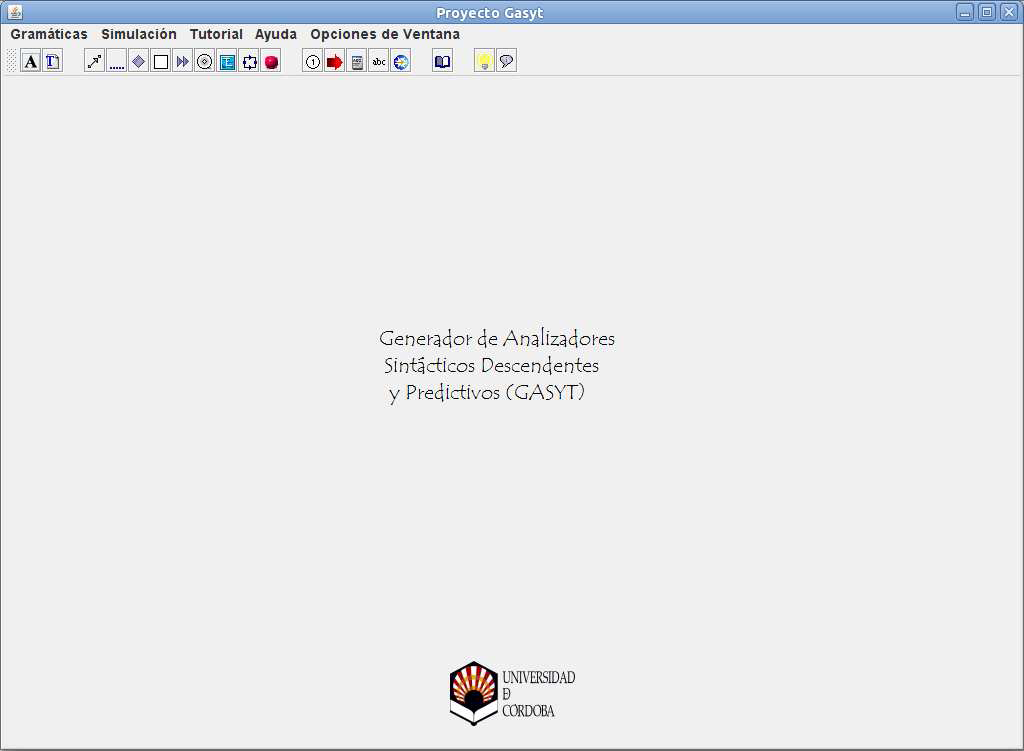
\includegraphics[scale=0.5]{img/GASYT.png} 
      \caption{GASYT}
      \label{Figura3_1_}
	\end{center}
  \end{figure}

\subsection{Proyecto SimLR}

\begin{itemize}

\item \textbf{T�tulo:} Simulador de An�lisis Sint�ctico Ascendente LR. [Figura \ref{Figura3_2_}]

\item \textbf{Autor:} Luis del Moral Mart�nez. Universidad de C�rdoba.

\item \textbf{Descripci�n:} este proyecto tambi�n esta desarrollado en lenguaje Java, el cual realiza una simulaci�n del an�lisis sint�ctico Ascendente. Consta de la siguiente funcionalidad:
	\begin{itemize}
	\item Creaci�n de gram�ticas de contexto libre.
	\item Explicaci�n de los m�todos de \textit{An�lisis LR}.
	\item Simulaci�n de los m�todos de \textit{An�lisis LR}.
	\end{itemize}

\item \textbf{Requisitos:} el �nico requisito es contar con la m�quina virtual de Java.

\end{itemize}
 

\begin{figure}
	\begin{center}
     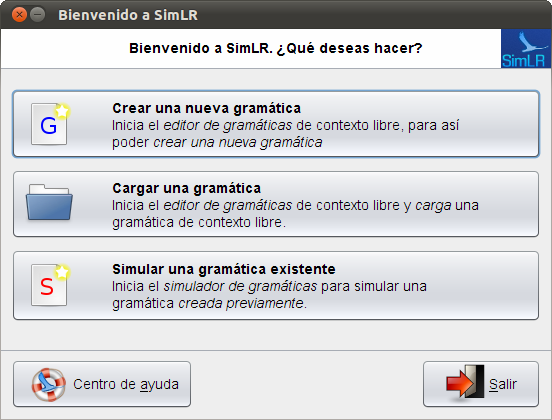
\includegraphics[scale=0.5]{img/SimLR.png} 
      \caption{SimLR}
      \label{Figura3_2_}
	\end{center}
  \end{figure}


\section{Justificaci�n del proyecto}

La implementaci�n de \textit{SimAS} se encuentra justificado por las siguientes razones: [tabla \ref{tlb:tabla3_1}]

\begin{itemize}

\item El an�lisis sint�ctico es la fase m�s compleja en la construcci�n de un compilador y su estudio resulta bastante tedioso.

\item El simulador ser� de gran ayuda para el aprendizaje paso a paso del an�lisis sint�ctico.

\item No existe ninguna herramienta que a�ne ambos tipos de an�lisis sint�ctico, descendente y ascendente.
\end{itemize}

Por todo lo descrito anteriormente, se ha cre�do conveniente llevar a cabo este proyecto de �mbito did�ctico, cumpliendo todos los objetivos expuestos en el cap�tulo anterior y que cubra las necesidades del usuario final.

 
\begin{center}

\begin{table}[H]

 \caption{Comparaci�n entre proyectos}

\resizebox{15cm}{!} {
\begin{tabular}[c]{| l | c | c | c |}
\hline
  & \textbf{GASYT} & \textbf{SimLR} & \textbf{SimAS} \\ \hline
 Generaci�n de gram�ticas de contexto libre & S� & S� & S� \\ \hline
 An�lisis sint�ctico descendente & S� & No & S� \\ \hline
 An�lisis sint�ctico ascendente & No & S� & S� \\ \hline
 Tutorial & S� & S� & S� \\ \hline
 Ayuda & S� & S� & S� \\ \hline
 Generaci�n de informes & S� & S� & S� \\ \hline
 Detecci�n y recuperaci�n de errores & No & S� & S� \\ \hline

\end{tabular}
}

 \label{tlb:tabla3_1}

\end{table}

\end{center}


\chapter{Restricciones}

\section{Introducci�n}

En este cap�tulo se expondr�n todas las restricciones, o factores limitativos, existentes en el �mbito del dise�o y que condicionan la elecci�n de una u otra alternativa.\\

Los factores limitativos pueden estructurarse en dos grupos:

\begin{itemize}

\item \textbf{Factores iniciales:} son aquellos que no pueden ser modificados durante el transcurso del proyecto, como puede ser el presupuesto econ�mico asignado al proyecto o la duraci�n estimada del mismo.

\item \textbf{Factores estrat�gicos:} representan variables de dise�o que permiten la elecci�n entre diferentes alternativas por parte del desarrollador. En funci�n de la opci�n escogida, podr� alterarse el proceso de desarrollo y el propio producto final obtenido, con lo que resultar� necesario analizar las posibilidades existentes en las primeras etapas del proceso.

\end{itemize}

\section{Factores iniciales}

Las decisiones y aspectos iniciales a tener en cuenta a la hora de comenzar el proyecto son los siguientes:

\begin{itemize}

\item La aplicaci�n debe ser eficiente y robusta.

\item Aplicaci�n Multiplataforma: la aplicaci�n debe ser multiplataforma, esto es, que pueda ser instalado en cualquier sistema operativo, ejecut�ndose con las mismas prestaciones.

\item Enfoque did�ctico: el fin de esta herramienta es puramente did�ctico, por lo que debe facilitar la labor de aprendizaje paso a paso al usuario. Para ello, la aplicaci�n contar� con:
	\begin{itemize}
		\item En el men� de ayuda se explicar� cada uno de los m�todos de an�lisis sint�ctico.
		\item El tutorial de la aplicaci�n ayudar� al usuario a utilizarla.
	\end{itemize}
	
\item Introducci�n de datos: debe ser f�cil, manejable y c�moda para que el usuario no emplee demasiado tiempo en introducir los datos precisos que se exigen.

\item Interfaz Gr�fica: la interfaz debe ser simple y amigable, con el objetivo de facilitar el uso de la aplicaci�n. El simulador incluir� los elementos t�picos: men�s, submen�s, barras de herramientas, barrasd de estado, etc.

\item El simulador deber� realizar una representaci�n fidedigna y fiable de las operaciones o problemas que el usuario desee resolver.

\item Control de eventos: el programa deber� controlar todos los eventos que se produzcan durante la ejecuci�n. �stos se mostrar�n al usuario directamente, junto a un c�digo que identifique el tipo de error cometido.

\item Generaci�n de informes: los usuarios podr�n generar informes de las gram�ticas creadas as� como de las simulaciones. Estos informes se generar�n en formato PDF y se podr�n imprimir o guardar.

\end{itemize}

Esta informaci�n ser� ampliada en el \textit{Cap�tulo 6: Especificaci�n de requisitos}.

\section{Factores estrat�gicos}

En este apartado, se mostrar�n las decisiones estrat�gicas tomadas por el desarrollador para llevar a cabo el proyecto:

\begin{itemize}

\item Metodolog�a de desarrollo.
\item Elecci�n del lenguaje de programaci�n.
\item Elecci�n del entorno de desarrollo.
\item Desarrollo de la interfaz gr�fica de la aplicaci�n.
\item Elecci�n del Sistema Operativo para la implementaci�n.
\item Representaci�n de las gram�ticas de contexto libre.
\item Representaci�n de los informes de gram�ticas y de simulaci�n.
\item Implementaci�n de la ayuda.
\item Implementaci�n del tutorial.

\end{itemize}

\subsection{Metodolog�a de desarrollo}

Actualmente existen varias metodolog�as para el desarrollo de proyectos, como pueden ser:

\begin{itemize}
 \item \textbf{Ciclo de vida cl�sico o en cascada}: este modelo es el
    modelo cl�sico de desarrollo software por cascada. El modelo, ya en desuso, consiste en 
    llevar a cabo un desarrollo lineal del proyecto, de forma tal que 
    para pasar a la siguiente fase debe de haber terminado y estar 
    validada la anterior. 

 \item \textbf{Metodolog�a OMT (\textit{Object Modeling Technique})}:
    aunque puede ser utilizado para cualquier desarrollo de software,
    ha quedado en desuso y ha sido reemplazado por UML.

 \item \textbf{Notaci�n UML (\textit{Unified Modelling Language})}:
    el lenguaje de modelado unificado, o UML, es el m�s adecuado para el desarrollo
    de este proyecto, puesto que presenta orientaci�n a objetos, un lenguaje de modelado
    y t�cnicas que facilitan la extracci�n de requisitos. Adem�s, permite
    ser f�cilmente traducido a un lenguaje de alto nivel orientado a
    objetos (como C++, Java, Python, etc�tera). Este lenguaje unifica
    las t�cnicas de Booch, Jacobson y Rumbaugh (OMT).
\end{itemize}

Finalmente, se ha optado por utilizar \textbf{UML}, debido a que es el lenguaje gr�fico de modelado de sistemas software m�s conocido y utilizado en la actualidad. Se trata de un lenguaje de modelado que ofrece una alta capacidad de representaci�n en los lenguajes de alto nivel orientados a objetos que existen en
la actualidad.


\subsection{Elecci�n del lenguaje de programaci�n}

Es bien sabido que en la actualidad existen m�ltiples lenguajes de programaci�n que ofrecen grandes prestaciones para realizar aplicaciones de escritorio, como por ejemplo:

\begin{itemize}
\item \textbf{C++:} es un lenguaje multiparadigma y orientado a
   objetos, que a�ade programaci�n gen�rica e interfaces gr�ficas de usuario. Este lenguaje tiene la desventaja de que los programas deben ser compilados para la m�quina en la que se van a ejecutar,  adem�s de tener que depender de librer�as externas para poder representar las interfaces.
   
  \item \textbf{Python:} es un lenguaje interpretado y multiparadigma. Su principal caracter�stica es que es un lenguaje con una sintaxis muy limpia y que favorece un c�digo legible. En cambio, pueden 
   existir problemas de compatibilidad entre las plataformas Windows y Linux en ciertos aspectos, adem�s de depender de librer�as o lenguajes de programaci�n externos.
   
   \item \textbf{Java:} este lenguaje es orientado a objetos, proporciona mecanismos propios para la construcci�n de interfaces y adem�s es multiplataforma, debido a la M�quina Virtual de Java. �sta se abstrae de la arquitectura de hardware del computador y ejecuta el programa siempre de la misma forma sin importar el sistema operativo que se utilice. 
\end{itemize}

Tras comparar todas las opciones expuestas anteriormente, se ha decidido que la mejor opci�n para desarrollar este proyecto es utilizar el \textbf{lenguaje de programaci�n Java}. La raz�n principal es debido a su potente M�quina Virtual que permite la portabilidad.


\subsection{Elecci�n del entorno de desarrollo}

Despu�s de elegir el lenguaje de programaci�n Java para el desarrollo del proyecto, se presentan dos posibles entornos para llevarlo a cabo: NetBeans y Eclipse. Estas dos opciones son bastante competentes, sin embargo, se ha decidido utilizar NetBeans debido a que incluye componentes para la creaci�n de interfaces gr�ficas con Swing, lo que facilitar� la labor de la creaci�n de la interfaz de la aplicaci�n software.\\

El entorno \textbf{NetBeans} se presenta como un entorno multiplataforma de c�digo abierto, el cual integra un editor de texto avanzado y un int�rprete propio del lenguaje Java. Este programa pone a disposici�n de los programadores varias caracter�sticas que ayudan al desarrollo de sistemas inform�ticos:


\begin{itemize}

\item Resaltado de elementos del c�digo fuente.
\item Gesti�n de paquetes de c�digo fuente.
\item Control de errores sint�cticos y sem�nticos.
\item Entorno de depuraci�n de la aplicaci�n.
\item Editores de interfaces gr�ficas.
\item Plugins de creaci�n de ficheros .jar (ejecutables).

\end{itemize}


\subsection{Desarrollo de la interfaz gr�fica de la aplicaci�n}

Para el desarrollo de la interfaz gr�fica de la aplicaci�n existen varias interfaces de programaci�n, como puede ser \textit{AWT} y \textit{Swing}. 

Se ha decidido utilizar el paquete de interfaces gr�ficas de \textbf{Java} \textit{\textbf{javax.swing}}, el cual ofrece un conjunto de componentes escritos en Java con m�s y mejores funcionalidades, con la independencia de plataforma que propone la tecnolog�a Java. Se podr�n crear interfaces gr�ficas con los siguientes componentes: botones, ventanas, cuadros de texto, tablas, ... Este paquete permite crear interfaces gr�ficas de forma sencilla y con un acabado profesional, permitiendo en todo momento la personalizaci�n de cada uno de los componentes que lo integran.

\subsection{Elecci�n del sistema operativo para la implementaci�n}

Aunque la implementaci�n del proyecto se va a llevar a cabo mediante el lenguaje Java, el cual es totalmente portable, se ha elegido para su desarrollo el sistema operativo \textbf{Ubuntu 12.10}. A�n as�, la aplicaci�n se ir� probando simult�neamente durante su desarrollo en el sistema operativo Windows 7 bajo la misma m�quina virtual de Java.

\subsection{Representaci�n de las gram�ticas de contexto libre}

Para almacenar la informaci�n de las gram�ticas de contexto libre creadas por el usuario, existen varias opciones como por ejemplo: ficheros de texto plano, ficheros binarios, ficheros XML, ...\\

De entre estas posibilidades, se ha elegido el \textbf{lenguaje XML} debido a que permite definir un formato concreto para almacenar los datos de forma segura, cumpli�ndose adem�s que �stos puedan ser visualizados por el usuario y recuperados por el programa, siempre y cuando se siga el mismo formato de los datos. Con esto, ser� mucho m�s f�cil poder controlar todos los errores que se produzcan en el mismo.

\subsection{Generaci�n de informes de gram�ticas y de simulaci�n}

Para cada gram�tica creada con la aplicaci�n, se podr� generar un informe de la gram�tica, el cual contendr� toda la informaci�n sobre la misma. Tras la realizaci�n de una simulaci�n, se le dar� la opci�n al usuario de generar informes con los resultados de la simulaci�n, incluyendo todos los diagramas que se hayan generado.

Las alternativas para la generaci�n de informes son las siguientes: fichero de texto plano, PDF, ... Se ha decidido que los informes se generar�n en formato \textbf{PDF}, de esta forma no se podr� modificar el contenido del mismo.

\subsection{Implementaci�n de la ayuda}

La implementaci�n de la ayuda del programa se podr� llevar a cabo mediante un fichero de texto, un documento PDF o una p�gina web en cualquier lenguaje de programaci�n.

�sta se realizar� mediante una \textbf{p�gina Web desarrollada en lenguaje HTML}. Esta elecci�n se ha llevado a cabo debido a la capacidad que tiene Java de integrar c�digo fuente de otros lenguajes. Por esto, es muy sencillo incorporar p�ginas Web escritas en HTML dentro de componentes de la interfaz de Java. De esta forma, se pretende crear la ayuda en formato de p�ginas Web, para que sea cargada por componentes de la interfaz y el usuario navegue por dichas p�ginas. 

\subsection{Implementaci�n del tutorial}

El tutorial se realizar� en formato \textbf{PDF} y se proporcionar� junto con la aplicaci�n. Este explicar� los conceptos te�ricos del an�lisis sint�ctico, junto con ejercicios pr�cticos para afianzar los conceptos.\\

El hecho de estar realizado en PDF permite futuras modificaciones, ampliaciones o correcciones del tutorial.



\chapter{Recursos}

En este cap�tulo se expondr�n de forma clara y concisa los recursos humanos y materiales necesarios para este proyecto. Los recursos se definen como aquellos medios de los que se dispone para abordar el proceso de desarrollo del proyecto.\\

Los recursos se encuentran agrupados en tres grupos:
\begin{itemize}

\item Recursos humanos.
\item Recursos de hardware.
\item Recursos de software.

\end{itemize}

\section{Recursos humanos}

\begin{itemize}

\item Direcci�n y coordinaci�n: Dr. Nicol�s Luis Fern�ndez Garc�a. Profesor Titular de Universidad del �rea de conocimiento de Ciencias de la Computaci�n e Inteligencia Artificial. Departamento de Inform�tica y An�lisis Num�rico, Escuela Polit�cnica Superior de C�rdoba, Universidad de C�rdoba.

\item An�lisis, dise�o, programaci�n y documentaci�n: Vanesa Gonz�lez P�rez. Alumna de la titulaci�n Ingenier�a Inform�tica, Escuela Polit�cnica Superior de C�rdoba, Universidad de C�rdoba. 

\end{itemize}

\section{Recursos de Hardware}

Los recursos hardware se pueden subdividir en dos categor�as:

\begin{itemize}

\item Recursos de hardware para el desarrollo del proyecto: necesarios para llevar a cabo el desarrollo de la aplicaci�n. 

	\begin{itemize}
	
	\item Ordenador port�til Asus PRO5IJSeries. Intel Core i3-370M, 2,4 GHz. 4 GB de memoria RAM. HDD de 500 GB. Tarjeta gr�fica Radeon HD 6370m.	
	
	\end{itemize}
	
\item Recursos hardware para el uso de la aplicaci�n: requisitos m�nimos recomendados para el buen funcionamiento de la aplicaci�n.

	\begin{itemize}
	\item Requisitos m�nimos declarados por Sun Microsystems para que la M�quina Virtual de Java pueda funcionar correctamente.
	\end{itemize}
	
\end{itemize}		
	

\section{Recursos de Software}

\begin{itemize}

\item Sistemas operativos:
	\begin{itemize}
	\item Ubuntu Linux, versi�n 12.10
	\item Microsoft Windows 7
	\end{itemize}	 

\item Int�rpretes: Java SE (JDK) 7u40
\item Editores: editor de textos Texmaker para Latex
\item Programaci�n y planificaci�n del proyecto: gestor de proyectos OpenProj, para gestionar la organizaci�n temporal y la planificaci�n.
\item Entornos de desarrollo. NetBeans 7.3.1. Se utilizar� para la codificaci�n y pruebas de la aplicaci�n.
\item Herramientas de diagramado: se utilizar� el editor de diagramas Dia para desarrollar todos los diagramas del proyecto (diagramas de casos de uso, de clases, etc.).

\end{itemize}

\part{An�lisis}


\chapter{Especificaci�n de requisitos}

En este cap�tulo se llevar� a cabo la especificaci�n de los requisitos
de \textit{usuario}, la especificaci�n de los requisitos \textit{funcionales} y \textit{no funcionales}, as� como los requisitos de \textit{informaci�n} del programa que se pretende desarrollar.

En primer lugar, antes de empezar con la especificaci�n de los requisitos, se va a realizar la descripci�n funcional del simulador, especificando cada uno de los m�dulos identificados en los cap�tulos anteriores. Una vez hecho esto, ser� necesario definir los actores, es decir, los usuarios finales que har�n uso de la aplicaci�n.


\section{Descripci�n modular del Sistema}

A continuaci�n, en las siguientes subsecciones, se proceder�
a analizar detalladamente cada uno de los m�dulos que compondr�n
la aplicaci�n. Estos m�dulos se identificaron en los cap�tulos
anteriores y son los siguientes:

\begin{itemize}
 \item Editor de gram�ticas.
 \item Simulador:
 \begin{itemize}
 	 \item Simulador gr�fico descendente.
 	 \item Simulador gr�fico ascendente.
 
 \end{itemize}

 \item Tutorial.
 \item Ayuda.
\end{itemize}

En la Figura \ref{Figura61} se muestra la descomposici�n modular del Sistema.
\begin{figure}[H]
  \begin{center} 
    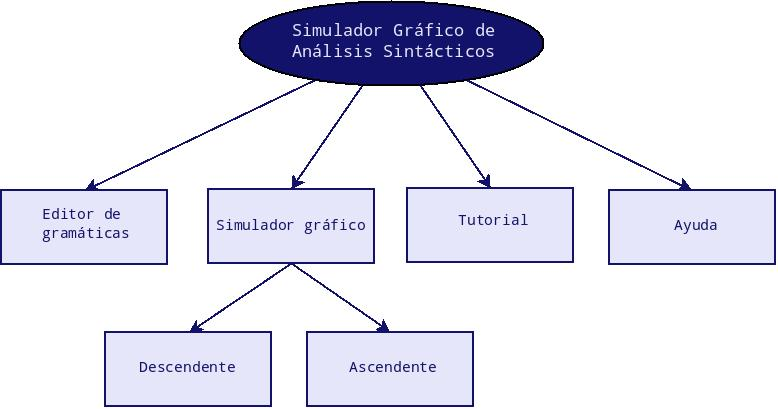
\includegraphics[width=1\textwidth]{img/descomp.jpg}
    \caption{Descomposici�n modular del Sistema}
    \label{Figura61}
  \end{center}
\end{figure}

\subsection{M�dulo \textit{Simulador Gr�fico de An�lisis Sint�cticos}}

Este es el m�dulo principal de la aplicaci�n. Contiene todos los dem�s
m�dulos, as� como los mecanimos para inicializar la aplicaci�n
y toda la interfaz.

A trav�s de este m�dulo, el usuario puede acceder a las funcionalidades
que proporcionan los dem�s m�dulos.

\subsection{M�dulo \textit{Editor de gram�ticas}}

Este m�dulo se encarga de la creaci�n y manipulaci�n de las gram�ticas de
contexto libre. Las funcionalidades que brinda este m�dulo son las siguientes:

\begin{enumerate}
 \item \textbf{Creaci�n de una gram�tica}: permitir� crear una gram�tica
  desde cero, creando cada uno de los componentes que la forman
  (vocabulario de s�mbolos, s�mbolo inicial y producciones).
 \item \textbf{Gesti�n del vocabulario de una gram�tica}: permitir� al usuario
  manipular el vocabulario de s�mbolos de la gram�tica (para a�adir o eliminar s�mbolos). Estos
 s�mbolos se emplear�n para crear las reglas de la gram�tica.
 \item \textbf{Gesti�n de producciones}: esta funcionalidad permitir� al usuario
  introducir todas las producciones  que componen la gram�tica.
  Se deber� tener en cuenta que no se
  puede tener dos instancias de la misma producci�n en la gram�tica. 
 \item {\textbf{Validaci�n}: esto permitir� al usuario validar una gram�tica
  creada o cargada de un fichero. De esta forma, se garantizar� que
  dicha gram�tica soporta un an�lisis sint�ctico. Algunas de las comprobaciones
  que este m�dulo llevar� a cabo ser�n las siguientes:
    \begin{enumerate}
      \item Comprobaci�n de la regla inicial de la gram�tica 
        (de la forma $S \rightarrow \dots$).
      \item Comprobaci�n de s�mbolos no terminales (comprobar que
	todos tienen al menos una producci�n asociada).
    \end{enumerate}
  En el caso de que la gram�tica no pueda ser validada, se deber�
  informar al usuario acerca de los posibles errores existentes
  y de la forma m�s adecuada de subsanarlos.}
 \item \textbf{Almacenamiento}: permitir� almacenar una gram�tica
  en un fichero en el disco. Este almacenamiento
  solo se podr� llevar a cabo siempre y cuando la gram�tica
  se haya validado de forma satisfactoria.
 \item \textbf{Carga}: permitir� cargar una gram�tica desde un fichero en el disco.
  Se deber� comprobar si el fichero a cargar es correcto y no es 
  corrupto, mostrando al usuario todos los errores que se puedan
  producir durante la carga de la gram�tica.
 \item \textbf{Representaci�n}: esta funcionalidad permitir� representar 
  la gram�tica visualmente, de forma intuitiva. Se utilizar� para
  mostrar al usuario la gram�tica de la misma forma que �ste la
  representar�a (te�ricamente hablando), y cumpliendo todas
  las convenciones de notaci�n (expuestas en el Anexo A de
  este documento).
 \item \textbf{Generaci�n de informes}: esta funcionalidad permitir� generar
un informe de la gram�tica, que contenga todos los componentes que la forman, adem�s
de una representaci�n gr�fica de la misma.
\end{enumerate}

\subsection{M�dulo \textit{Simulador Gr�fico}}

Este m�dulo es el punto central del proyecto. Se encargar� de la
simulaci�n de cada uno de los m�todos del an�lisis sint�ctico. Este m�dulo se divide en dos partes: Simulaci�n descendente y Simulaci�n ascendente. Ambos, tomar�n una gram�tica (creada con el m�dulo editor de gram�ticas) y realizar� la simulaci�n del m�todo elegido.

\subsubsection{Simulador descendente}

Los pasos a seguir para llevar a cabo la simulaci�n son los siguientes:

\begin{enumerate}
 \item \textbf{Creaci�n o carga de una gram�tica}: en primer lugar,
  el usuario crear� o cargar� una gram�tica, haciendo uso
  del m�dulo editor de gram�ticas. Se presupone que la gram�tica
  ha sido validada antes de cargarla en el simulador.
  
 \item \textbf{Conjuntos Primero y Siguiente}: el primer paso a dar con la gram�tica es la realizaci�n de los conjuntos primero y siguiente. Estos conjuntos permitir�n elegir la producci�n que se va a aplicar, con base en el siguiente s�mbolo de entrada.
  
 \item \textbf{Construcci�n de la tabla predictiva}: en este paso, se construir�
  la tabla predictiva del m�todo. Durante la construcci�n, se mostrar�n 
  al usuario todos los errores identificados. 
  
 \item \textbf{Simulaci�n}: una vez generada la tabla predictiva, el usuario podr�
  introducir una cadena de entrada y simularla seg�n dicha tabla. Nuevamente, se
  deber�n controlar todos los errores que se produzcan, as� como
  notificar al usuario si la cadena de entrada es o no reconocida.
  Durante la simulaci�n, el usuario podr� asignar ciertas funciones de tratamiento de errores, 
  para tratar los errores que se produzcan al reconocer la cadena.
  
 \item {\textbf{Generaci�n de informes}: por �ltimo, se generar�
  un informe de la simulaci�n realizada, el cual se podr� obtener en formato pdf o html. Este informe, que podr�
  ser guardado por el usuario en el disco, contendr� lo siguiente:
    \begin{itemize}
     \item Informaci�n sobre la gram�tica a simular.
     \item Conjuntos Primero y Siguiente.
     \item Tabla predictiva obtenida (incluyendo todos aquellos datos
      necesitados para calcularla).
     \item Cadena de entrada reconocida.
     \item Errores producidos y tratamiento realizado (si se producen).
    \end{itemize}
 }
\end{enumerate}


\subsubsection{Simulador ascendente}

Los pasos a seguir para llevar a cabo la simulaci�n son los siguientes:

\begin{enumerate}
 \item \textbf{Creaci�n o carga de una gram�tica}: al igual que en el caso anterior,
  el usuario crear� o cargar� una gram�tica, haciendo uso
  del m�dulo editor de gram�ticas. Se presupone que la gram�tica
  ha sido validada antes de cargarla en el simulador.
  
  \item \textbf{Selecci�n del m�todo de la simulaci�n}: a continuaci�n, se seleccionar� el m�todo con el que se realizar� la simulaci�n: \textit{SLR, LR-can�nico o LALR}.
  
  \item \textbf{Conjuntos Primero y Siguiente}: en el caso de que el m�todo de simulaci�n elegido sea \textit{SLR}, ser� necesario la construcci�n de los conjuntos Primero y Siguiente.
  
 \item \textbf{Construcci�n de la tabla de an�lisis LR}: en este paso, se construir�
  la tabla LR del m�todo seleccionado. Durante la construcci�n, se mostrar�n 
  al usuario todos los errores identificados. 
  
 \item \textbf{Simulaci�n}: una vez generada la tabla LR correspondiente, el usuario podr�
  introducir una cadena de entrada y simularla seg�n dicha tabla. Nuevamente, se
  deber�n controlar todos los errores que se produzcan, as� como
  notificar al usuario si la cadena de entrada es o no reconocida.
  Durante la simulaci�n, el usuario podr� asignar ciertas funciones de tratamiento de errores, 
  para tratar los errores que se produzcan al reconocer la cadena.
  
 \item {\textbf{Generaci�n de informes}: por �ltimo, se generar�
  un informe de la simulaci�n realizada, el cual se podr� obtener en formato pdf o html. Este informe, que podr� ser guardado por el usuario en el disco, contendr� lo siguiente:
    \begin{itemize}
     \item Informaci�n sobre la gram�tica a simular.
     \item Conjuntos Primero y Siguiente si el m�todo de simulaci�n es \textit{SLR}.
     \item Tabla de an�lisis LR obtenida (incluyendo todos aquellos datos
      necesitados para calcularla).
     \item Cadena de entrada reconocida.
     \item Errores producidos y tratamiento realizado (si se producen).
    \end{itemize}
 }
\end{enumerate}



\subsection{M�dulo \textit{Tutorial}}

Este m�dulo se encargar� de cubrir todos los objetivos did�cticos
del proyecto. Para ello, se situar� este m�dulo de forma que sea
accesible desde los dem�s m�dulos del programa. As�, el usuario
podr� consultarlo cuando desee, incluso a la vez que trabaja con
el programa.


El tutorial constrar� de las siguientes partes:

\begin{enumerate}
 \item \textbf{Introducci�n y conceptos te�ricos b�sicos}: esta secci�n
  del tutorial tratar� de los conceptos te�ricos en los que se
  basa el an�lisis sint�ctico, as� como las gram�ticas
  de contexto libre.
  \item \textbf{Lecciones de an�lisis sint�ctico descendente}: en esta secci�n
  se explicar�n los m�todos de an�lisis sint�ctico descendente predictivo, paso a paso.
 \item \textbf{Lecciones de an�lisis sint�ctico ascendente}: en esta secci�n
  se explicar�n los tres m�todos de an�lisis LR, paso a paso.
 \item \textbf{Ejemplos y ejercicios propuestos}: finalmente, esta secci�n
  contendr� ejercicios propuestos para los usuarios. Por medio de esta
  secci�n, los usuarios podr�n realizar los ejercicios y comprobarlos
  con el simulador. Esto facilitar� mucho la tarea de aprendizaje del alumnado.
\end{enumerate}


\subsection{M�dulo \textit{Ayuda}}

Este m�dulo cubrir� la ayuda de la aplicaci�n. En esta ayuda,
se detallar� el funcionamiento de cada uno de los m�dulos de la aplicaci�n.
Los contenidos de la ayuda son los siguientes:

\begin{enumerate}
 \item \textbf{Introducci�n}: este cap�tulo introducir� al usuario
  al software, exponiendo los objetivos del mismo.
 \item \textbf{Instalaci�n y desinstalaci�n}: este cap�tulo detallar�
  los requisitos necesarios del programa, as� como la instalaci�n
  y desinstalaci�n del mismo.
 \item \textbf{Interfaz del programa}: este cap�tulo explicar� al usuario
  los diferentes componentes que forman la interfaz del simulador.
 \item \textbf{M�dulos del programa}: este cap�tulo tratar� con profundidad
  el funcionamiento de cada uno de los m�dulos del programa.
 \item \textbf{Resoluci�n de problemas y c�digos de error}: finalmente, este cap�tulo estar�
  orientado a la resoluci�n de errores, as� como a la explicaci�n
  en profundidad de los errores producidos en el programa. 
\end{enumerate}


\section{Especificaci�n de los actores del Sistema}

Se ha decidido especificar el actor del Sistema
en este cap�tulo, puesto que es necesario antes de especificar
cada uno de los requisitos de usuario y funcionales que se derivan
de estos m�dulos.

Como ya se ha comentado en apartados anteriores, el software que se quiere desarrollar
tiene una finalidad docente. Debido a esto, estar� dirigido a dos tipos de usuarios: \textit{profesores} y \textit{alumnos}. A la hora de usar la aplicaci�n no habr� distinci�n entre unos y otros porque ambos har�n el mismo uso, por tanto solamente se tendr� en cuenta un �nico tipo de usuario final. As�, en posteriores cap�tulos, cuando se haga referencia al 
\textit{actor} de la aplicaci�n, deber� tenerse en cuenta lo comentado en este apartado.

\section{Requisitos de usuario}

En este apartado se recogen los requisitos del usuario; esto es, 
los requisitos que el usuario precisa en el Sistema. Puesto que solamente
existe un usuario (o actor) en el Sistema, todos los requisitos
que se muestran son para el mismo usuario. Los requisitos de
usuario se denotan como \textbf{RU-$<$ n�mero de requisito $>$}.

Los requisitos de usuario se encuentran agrupados por categor�as que se muestran a continuaci�n:

\begin{itemize}
 \item \textbf{Edici�n de gram�ticas}: requisitos de usuario relacionados
con la \textit{edici�n de gram�ticas de contexto libre}.
 \item \textbf{Simulaci�n}: requisitos de usuario relacionados
con la \textit{simulaci�n}, seg�n los m�todos sint�cticos descendentes y ascendentes, de gram�ticas
de contexto libre.
 \item \textbf{Tutorial de la aplicaci�n}: requisitos de usuario
referentes al \textit{tutorial} de la aplicaci�n.
 \item \textbf{Ayuda de la aplicaci�n}: requisitos de 
usuario de la \textit{ayuda} de la aplicaci�n.
\end{itemize}

\subsection{Edici�n de gram�ticas}

\textbf{RU-1}: el usuario podr� crear una gram�tica de contexto libre, adem�s podr� asignar un nombre y una descripci�n a la gram�tica. No deber� existir ninguna limitaci�n en el n�mero de gram�ticas que puede crear el usuario.

\textbf{RU-2}: una vez creada la gram�tica, el usuario podr�:


\begin{description}

\item [\hspace*{1.5cm} \textbf{RU-2.1}:] definir el vocabulario de s�mbolos terminales y no terminales
que componen la gram�tica. Estos s�mbolos podr�n ser definidos
seg�n los convenios de notaci�n que se especifican
en el Anexo A (permiti�ndose tambi�n el uso de la palabra vac�a
o $\epsilon$). \\

\item [\hspace*{1.5cm} \textbf{RU-2.2}:] se deber� permitir que el usuario pueda modificar el 
vocabulario de s�mbolos cuando lo desee, teniendo en cuenta tambi�n si estos
s�mbolos est�n asignados a reglas de producci�n o no
(informando al usuario adem�s de todos los errores que se produzcan).

\end{description}


\textbf{RU-3}: cuando el usuario haya creado el vocabulario de la gram�tica, podr� utilizar
los s�mbolos creados para crear cada una de las producciones de la gram�tica.


\textbf{RU-4}: el usuario podr� crear o editar las producciones
de la gram�tica, permiti�ndose adem�s el borrado
de las mismas. A la hora de crearlas o modificarlas,
el usuario podr� seleccionar los s�mbolos de entre el vocabulario
de la gram�tica, creados como se especifica en \textbf{RU-2}.
A partir de estos s�mbolos, el usuario podr� definir
el \textit{antecedente} y el \textit{consecuente} de la producci�n.

\textbf{RU-5}: el usuario podr� visualizar la gram�tica de forma 
\textit{natural}, a medida que la va creando. Un ejemplo de este hecho ser�a:
\begin{center}
 $<${\em asignaci�n}$>$ $\rightarrow$ {\em identificador}
{\em =} $<${\em expresi�n}$>$
\end{center}

\textbf{RU-6}: el usuario, una vez creadas las reglas de producci�n, podr� seleccionar de entre los s�mbolos no terminales cu�l ser� s�mbolo inicial de la gram�tica.

\textbf{RU-7}: el usuario podr� generar un informe de la gram�tica definida, con la que podr� visualizar la misma. Esta visualizaci�n representar� las producciones de la gram�tica como se especifica
en \textbf{RU-5}. Adem�s, este informe contendr� informaci�n detallada acerca del \textit{vocabulario}
de la gram�tica (s�mbolo inicial, producciones, terminales y
no terminales). Este informe podr� ser guardado en el disco duro si el usuario lo desea.


\textbf{RU-8}: el usuario podr� guardar una 
gram�tica previamente definida, con objeto de 
poder recuperarla posteriormente para trabajar con ella sin necesidad de volver a crearla.


\textbf{RU-9}: el usuario podr� recuperar una gram�tica guardada.

\textbf{RU-10}: el usuario podr� validar una gram�tica creada. As� se podr�
garantizar que la gram�tica puede ser utilizada en una simulaci�n
posterior. En el caso de que se produzcan errores, 
se deber�n notificar al usuario antes de continuar.
El usuario tambi�n ser� notificado en caso de que la
gram�tica sea validada con �xito. 


\textbf{RU-11}: el usuario podr� transferir una 
gram�tica al simulador y realizar una simulaci�n
con ella. El usuario solamente podr� transferir una gram�tica.


\subsection{Simulaci�n} 


\textbf{RU-12}: el usuario podr� seleccionar el mecanismo a simular, m�todo descendente o m�todo ascendente:

\begin{description}

\item [\hspace*{1.5cm} \textbf{RU-12.1}:] se obtendr� los conjuntos Primero y Siguiente.

\item [\hspace*{1.5cm} \textbf{RU-12.2}:] el usuario podr� obtener la tabla predictiva o la tabla LR correspondiente. 

\item [\hspace*{1.5cm} \textbf{RU-12.3}:] se construir�n todas las estructuras adicionales
necesarias para la simulaci�n:
\begin{itemize}
\item Conjuntos primero y siguiente.
\item Tabla predictiva (an�lisis sint�cticos descendente).
\item Tabla de an�lisis LR: tabla acci�n y tabla ir\_a (an�lisis ascendente LR).
\end{itemize}

\item [\hspace*{1.5cm} \textbf{RU-12.4}:] las tablas de an�lisis podr�n ser completadas
con las funciones de error que haya definido el usuario.

\end{description}


\textbf{RU-13}: el usuario podr� asignar funciones de tratamiento de error a las tablas de an�lisis:

\begin{description}

\item [\hspace*{1.5cm} \textbf{RU-13.1}:] el usuario podr� utilizar el \textit{m�todo de nivel
de frase} o el \textit{modo de p�nico} para ampliar las tablas. 

\item [\hspace*{1.5cm} \textbf{RU-13.2}:] el usuario podr� asignar un identificador a cada funci�n, para poderla diferenciar de las dem�s. 

\item [\hspace*{1.5cm} \textbf{RU-13.3}:] el usuario podr� asignar a las funciones un mensaje que las
describa y una acci�n a llevar a cabo cuando sean aplicadas y  un s�mbolo que ser� usado en la acci�n de la misma. De esta forma, el usuario podr� asignar a una gram�tica tantas funciones de error como desee (o ninguna).

\end{description}


\textbf{RU-14}: el usuario ser� informado de cualquier anomal�a o error que se produzca durante 
la generaci�n de la tablas de an�lisis.


\textbf{RU-15}: el usuario, una vez se hayan generado todos los elementos necesarios:

\begin{description}

\item [\hspace*{1.5cm} \textbf{RU-15.1}:] podr� simular el m�todo sint�ctico descendente.

\item [\hspace*{1.5cm} \textbf{RU-15.2}:] podr� simular los m�todos sint�cticos ascendentes LR, estos son \textit{SLR}, \textit{LR-can�nico} y \textit{LALR}. 

\end{description}


\textbf{RU-16}: el usuario podr� introducir una \textit{cadena de s�mbolos terminales}
para realizar el an�lisis. 

\begin{description}

\item [\hspace*{1.5cm} \textbf{RU-16.1}:] esta cadena deber� estar formada
por s�mbolos terminales de la gram�tica. 

\item [\hspace*{1.5cm} \textbf{RU-16.2}:] tambi�n se permite el uso de 
\textit{s�mbolos especiales}, tales como la palabra vac�a ($\epsilon$).

\end{description}


\textbf{RU-17}: una vez construidos los conjuntos Primero y Siguiente, la tabla de an�lisis y seleccionados
los s�mbolos terminales y no terminales, la simulaci�n se podr� realizar de paso a paso. 


\textbf{RU-18}: en la simulaci�n, se mostrar� al usuario
una tabla de an�lisis, que contendr� los resultados de la simulaci�n, adem�s de todos los
errores producidos y se notificar� si la cadena es reconocida o no.


\textbf{RU-19}: en la simulaci�n paso a paso, se construir� la
tabla de an�lisis fila a fila, informando al usuario
de los errores en el momento que se produzcan.


\textbf{RU-20}: el usuario ser� informado de todos los errores
que se pudieran producir durante la simulaci�n:

\begin{description}

\item [\hspace*{1.5cm} \textbf{RU-20.1}:] si el usuario ha definido funciones de tratamiento de error,
�stas deber�n de ser aplicadas. 

\item [\hspace*{1.5cm} \textbf{RU-20.2}:] el usuario deber� conocer en todo momento qu� funciones han sido aplicadas para solucionar los errores.

\end{description}


\textbf{RU-21}: El usuario obtendr� tras la simulaci�n:

\begin{description}

\item [\hspace*{1.5cm} \textbf{RU-21.1}:] un informe detallado de todos los pasos seguidos en formato pdf o html, as� como los resultados finales. 

\item [\hspace*{1.5cm} \textbf{RU-21.2}:] adem�s contendr� los conjuntos Primero y Siguiente, la tabla de an�lisis y todos los componentes auxiliares generados, as� como el proceso de an�lisis desarrollado. 

\item [\hspace*{1.5cm} \textbf{RU-21.3}:] tambi�n ser�n incluidos todos los errores que se hayan producido
durante la simulaci�n (as� como las funciones de error que se hayan utilizado).

\end{description}


\textbf{RU-22}: El usuario podr� guardar los \textit{informes de
simulaci�n} en el disco, para poder utilizarlos con posterioridad,
sin necesidad de abrir la aplicaci�n.


\textbf{RU-23}: el usuario podr� abortar la simulaci�n, para
cambiar la gram�tica o el m�todo a simular. El usuario deber� ser avisado de la p�rdida
de todo el trabajo realizado hasta el momento y deber� de poder
guardar todo el trabajo si lo desea.


\subsection{Tutorial de la aplicaci�n}


\textbf{RU-24}: el usuario podr� consultar un tutorial que
explique los procedimientos de An�lisis Sint�ctico. 


\textbf{RU-25}: el tutorial de la aplicaci�n se organizar� por lecciones:

\begin{description}

\item [\hspace*{1.5cm} \textbf{RU-25.1}:] deber� cubrir todo el proceso de an�lisis sint�ctico tanto ascendente como descendentecon sus diferentes m�todos. 

\item [\hspace*{1.5cm} \textbf{RU-25.2}:] el usuario podr� consultar
ejemplos que ilustren las explicaciones de cada secci�n.

\end{description}


\subsection{Ayuda de la aplicaci�n}


\textbf{RU-26}: el usuario podr� consultar una ayuda sobre la
aplicaci�n que detalle el funcionamiento de cada uno de los m�dulos
de del programa:

\begin{description}

\item [\hspace*{1.5cm} \textbf{RU-26.1}:] la ayuda contendr� informaci�n acerca de la
interfaz del programa y de los errores que se puedan producir
en tiempo de ejecuci�n. 

\item [\hspace*{1.5cm} \textbf{RU-26.2}:] la ayuda estar� organizada seg�n los m�dulos que componen la aplicaci�n, detallando adem�s el funcionamiento de la interfaz del mismo y un ejemplo de ejecuci�n.

\item [\hspace*{1.5cm} \textbf{RU-26.3}:] �sta no tratar� los puntos que aborde el tutorial de la aplicaci�n.

\end{description}


\section{Requisitos funcionales}

En esta secci�n se recogen los requisitos funcionales
de la aplicaci�n. Estos se derivan de los requisitos de usuario
de la secci�n anterior. Los requisitos se muestran
agrupados, seg�n los m�dulos ya identificados en la secci�n anterior
y se denotan como \textbf{RF-$<$acr�nimo del m�dulo$>$-$<$n�mero de requisito$>$}.


Los requisitos funcionales se encuentran agrupados
seg�n los m�dulos funcionales del Sistema, que son
las siguientes:

\begin{itemize}
 \item \textbf{M�dulo Editor de gram�ticas}: requisitos
funcionales del \textit{editor de gram�ticas}.
 \item \textbf{M�dulo Simulador}: requisitos funcionales
del \textit{simulador}.
 \item \textbf{M�dulo Tutorial}: requisitos funcionales
del \textit{tutorial}.
 \item \textbf{M�dulo Ayuda}: requisitos funcionales
del \textit{ayuda}.
\end{itemize}

\subsection{Requisitos funcionales del Editor de gram�ticas}

Esta secci�n recoge todos los requisitos funcionales del
\textit{Editor de gram�ticas}. Estos se enumeran a continuaci�n:


\textbf{RF-E-1}: el editor de gram�ticas permitir�
al usuario crear una gram�tica desde cero. El usuario
podr� crear o recuperar tantas gram�ticas como desee,
sin imponer ninguna restricci�n al n�mero de gram�ticas
que podr� estar editando a la vez el usuario. 

\textbf{RF-E-2}: el editor de gram�ticas permitir� la creaci�n y edici�n del vocabulario
de s�mbolos de la gram�tica (s�mbolos terminales y no terminales):

\begin{description}

\item [\hspace*{1.5cm} \textbf{RF-E-2.1}:] se contemplar� el uso
de caracteres especiales (expuestos en la nomenclatura del Anexo A), 
tales como los siguientes: $\epsilon$, $\rightarrow$, etc�tera.

\item [\hspace*{1.5cm} \textbf{RF-E-2.2}:] se podr�n definir s�mbolos propios para construir
dichas reglas (ejemplo: $<$asignaci�n$>$). 

\item [\hspace*{1.5cm} \textbf{RF-E-2.3}:] a cada s�mbolo especial
 de la gram�tica se le asignar� un c�digo especial (para
que lo distinga el simulador) y otro c�digo en \textit{unicode} (para facilitar
la representaci�n de \textit{forma natural}). 

\item [\hspace*{1.5cm} \textbf{RF-E-2.4}:] se controlar�n todos los errores asociados a la creaci�n
y edici�n de s�mbolos, notific�ndolos al usuario de la forma m�s clara y simple posible.

\end{description}


\textbf{RF-E-3}: el editor permitir� crear las reglas de producci�n, 
utilizando los s�mbolos de la gram�tica creados por el usuario. Adem�s, se comprobar� si el \textit{antecedente} de la misma es un \textit{�nico s�mbolo no terminal}.


\textbf{RF-E-4}: la inserci�n de reglas de producci�n estar� controlada
y se informar� al usuario de todos los errores que se produzcan.
As�mismo, si el usuario intenta introducir dos veces la misma
regla, el sistema lo notificar�, permiti�ndose solamente
una instancia de la misma.


\textbf{RF-E-5}: el editor de gram�ticas permitir� la edici�n de todas las
producciones introducidas, permiti�ndose modificar ambas partes
de la producci�n (antecedente y consecuente). Adem�s, se permitir�
borrar las producciones de la gram�tica.


\textbf{RF-E-6}: el s�mbolo inicial de la gram�tica se tomar�, por defecto, como 
el antecedente de la primera producci�n que haya introducido el usuario. 
A�n as�, el editor permitir� al usuario cambiarlo posteriormente si as� lo 
desea. La gram�tica solamente podr� tener un �nico s�mbolo inicial.


\textbf{RF-E-7}: la gram�tica tendr� asociada un nombre
y una descripci�n, los cuales introducir� el usuario
desde el propio editor de gram�ticas. Tanto el nombre como la 
descripci�n pueden ser modificados en cualquier momento.


\textbf{RF-E-8}: la gram�tica ser� visualizada en el editor
a medida que se vaya construyendo. As�, se ir� actualizando
con cada nueva regla que se introduzca. 


\textbf{RF-E-9}: el editor permitir�, generar un informe de la gram�tica actual.
Este informe contendr� toda la visualizaci�n y componentes de la misma, y podr�
ser guardado en el disco a petici�n del usuario. 


\textbf{RF-E-10}: el editor de gram�ticas permitir� cerrar la gram�tica
actual. Para ello, se notificar� al usuario de la acci�n y se
guardar� la gram�tica en curso, si el usuario lo desea
(evit�ndose todas las posibles p�rdidas de datos).


\textbf{RF-E-11}: la gram�tica actual podr� ser guardada en
el disco para su posterior uso. Se pedir� al usuario un 
nombre para el archivo y el lugar para almacenarlo, adem�s de un nombre para la gram�tica, en
caso de que no lo haya introducido.


\textbf{RF-E-12}: el editor de gram�ticas permitir� abrir una gram�tica
guardada en un fichero para as� cargarla en el editor. Se controlar�n todos 
los errores producidos por esta acci�n y se mostrar�n al usuario todos los 
errores producidos en caso de que no se pueda cargar la gram�tica.


\textbf{RF-E-13}: la validaci�n de la gram�tica comprobar�
que la gram�tica puede ser utilizada para realizar una simulaci�n.
En esta validaci�n se deber�n comprobar los siguientes aspectos:

   \begin{itemize}
    \item Solamente puede existir un s�mbolo inicial (seg�n lo especificado en \textbf{RF-E-6}).
    \item Todos los s�mbolos no terminales que aparezcan en el lado
    derecho de una regla (es decir, que est�n en el consecuente de una
    regla), deber�n aparecer al menos una vez en el lado izquierdo
    de alguna regla. (No puede haber s�mbolos no terminales
    que no tengan asociada ninguna regla de producci�n).    
    \item Todos los s�mbolos de la gram�tica, terminales y no terminales, deber�n
    ser usados en las producciones de la gram�tica.
   \end{itemize}

\textbf{RF-E-14}: los errores identificados durante la validaci�n
ser�n notificados al usuario. No se permitir� continuar con la
simulaci�n en caso de detectarse errores en la gram�tica. En caso
de que la validaci�n sea satisfactoria, se comunicar� al usuario
con un mensaje.


\textbf{RF-E-15}: el editor de gram�ticas permitir� transferir gram�ticas al 
simulador para realizar simulaciones de los m�todos de an�lisis sint�cticos. 
Solamente se podr�n transferir aquellas gram�ticas que hayan
sido validadas satisfactoriamente. Esta acci�n inicializar� el 
simulador y cargar� la gram�tica dentro del mismo para poder simularla.


\subsection{Requisitos funcionales del Simulador}

\textbf{RF-S-1}: el simulador permitir� que el usuario
seleccione el m�todo que desea simular, m�todo descendente o m�todo ascendente LR (\textit{SLR}, \textit{LR-can�nico} y \textit{LALR}).

\textbf{RF-S-2}: el simulador crear� los conjuntos Primero y Siguiente. Estos ser�n necesarios para el an�lisis sint�ctico descendente y para el m�todo SLR de an�lisis sint�ctico ascendente.

\textbf{RF-S-3}: el simulador construir� la \textit{tabla predictiva} o la 
\textit{tabla LR} y todos los elementos auxiliares necesarios para el m�todo 
seleccionado. El simulador permitir� adem�s completar dicha tabla con las 
funciones de error definidas por el usuario (en caso de que haya definido alguna).


\textbf{RF-S-4}: el simulador permitir� el uso
de funciones de tratamiento de error tanto en la tabla predictiva como en la tabla LR, 
seg�n el m�todo de nivel de frase o m�todo de p�nico. Adem�s, se permitir� al usuario
guardar estas funciones de error, para poder ser utilizadas m�s tarde en otra gram�tica
o en la misma gram�tica si as� lo desea.


\textbf{RF-S-5}: el simulador notificar� todos los errores
que se produzcan durante la creaci�n de las tablas.


\textbf{RF-S-6}: las funciones de error ser�n invocadas durante
la simulaci�n, cuando se produzca un error.


\textbf{RF-S-7}: el simulador permitir� que la simulaci�n
comience una vez se haya escogido un \textit{m�todo} y se haya generado
la \textit{tabla} correspondiente (tanto si est� completada por funciones 
de error como si no lo est�).


\textbf{RF-S-8}: el simulador pedir� al usuario una cadena de entrada para 
comprobar si es reconocida por el m�todo de simulaci�n. Dicha cadena podr�
tambi�n ser vac�a ($\epsilon$). Finalmente,
se deber�n controlar todos los posibles errores
de entrada-salida, o de simulaci�n, que pudieran suceder.


\textbf{RF-S-9}: una vez creada la tabla predictiva o la tabla LR e introducida
la cadena de entrada, se podr� iniciar la simulaci�n, de forma
continua o paso a paso.


\textbf{RF-S-10}: en la simulaci�n continuada, el simulador
mostrar� el resultado final de la simulaci�n en una tabla, conteniendo
adem�s todos los errores producidos. La tabla se generar� y se mostrar�
completa al usuario.


\textbf{RF-S-11}: en la simulaci�n paso a paso, el simulador
mostrar� el resultado de la simulaci�n paso a paso, construyendo
la tabla de resultado de forma \textit{incremental}, a medida que el usuario
solicite continuar la simulaci�n.


\textbf{RF-S-12}: el simulador informar� al usuario
de cualquier error que se produzca durante la simulaci�n. 
Si existen funciones de tratamiento de error asociadas, se 
utilizar�n, indicando al usuario el motivo de su uso.


\textbf{RF-S-13}: el simulador generar� un informe de simulaci�n
al finalizar en formato pdf o html. Este contendr� todas las estructuras
necesarias para llevar a cabo el an�lisis, as� como todos
los pasos seguidos durante el an�lisis (incluyendo todos
los errores producidos). 

\textbf{RF-S-14}: el simulador permitir� guardar los
informes de simulaci�n en el disco duro.


\textbf{RF-S-15}: las simulaciones podr�n ser abortadas, 
para as� poder cambiar la gram�tica, el m�todo a simular o
el conjunto de funciones de error.
Se deber� informar al usuario si quiere conservar todo el trabajo
realizado hasta ese punto y guardar los informes de simulaci�n
producidos (si los hay).


\subsection{Requisitos funcionales del Tutorial}


\textbf{RF-T-1}: el tutorial ser� accesible
al usuario desde cualquier ventana de la aplicaci�n.


\textbf{RF-T-2}: el tutorial se organizar� en lecciones, de forma tal 
que cubran todo el proceso de operaci�n con los mecanismos del an�lisis sint�ctico.


\subsection{Requisitos funcionales de la Ayuda}


\textbf{RF-A-1}: la ayuda de la aplicaci�n ser� accesible
desde cualquier ventana de la aplicaci�n.


\textbf{RF-A-2}: la ayuda de la aplicaci�n se estructurar� en cap�tulos, 
que contendr�n ayuda sobre todos los m�dulos que componen la aplicaci�n. 
Adem�s, se deber� explicar paso a paso todos los procedimientos que se 
pueden llevar a cabo en ellos, utilizando para ello ejemplos de uso.


\section{Requisitos no funcionales}

En esta secci�n se recogen los requisitos no funcionales
del Sistema. Estos se denotan como \textbf{RNF-$<$n�mero de requisito$>$}.


\textbf{RNF-1}: la interfaz del Sistema deber� de ser sencilla y siempre 
estar enfocada al objetivo prioritario de la transmisi�n did�ctica del 
an�lisis sint�ctico. Para ello, se emplear�n men�s intuitivos, as� como 
botones de acci�n e im�genes enfocados a los m�todos del an�lisis sint�ctico.


\textbf{RNF-2}: la aplicaci�n deber� controlar
todos los errores que se produzcan durante la ejecuci�n
(errores de entrada-salida, de ejecuci�n, de simulaci�n,
etc�tera).

\textbf{RNF-3}: el sistema deber� responder en un tiempo aceptable a las peticiones del usuario.



\section{Requisitos de la informaci�n}

En esta secci�n se recogen los requisitos de la informaci�n. 
�stos se denotan como \textbf{RI-$<$acr�nimo del m�dulo$>$-$<$n�mero de requisito$>$}.
Los requisitos se encuentran agrupados por conceptos identificados
en el problema t�cnico o durante la especificaci�n de los requisitos de usuario.

Los requisitos de la informaci�n se agrupan 
seg�n los siguientes \textit{bloques de informaci�n}:

\begin{itemize}
 \item \textbf{Gram�tica de contexto libre}: requisitos
de informaci�n del m�dulo \textit{gram�tica de contexto libre}.
 \item \textbf{Editor de gram�ticas}: requisitos
de informaci�n del m�dulo \textit{editor de gram�ticas}.
 \item \textbf{Simulador}: requisitos
de informaci�n del m�dulo \textit{simulador}.
 \item \textbf{Ayuda de la aplicaci�n}: requisitos
de informaci�n del m�dulo \textit{ayuda de la aplicaci�n}.
 \item \textbf{Tutorial de la aplicaci�n}: requisitos
de informaci�n del m�dulo \textit{tutorial de la aplicaci�n}.
 \item \textbf{Informes}: requisitos
de informaci�n del m�dulo \textit{informe de gram�tica}
y \textit{informe de simulaci�n}.

\end{itemize}

\subsection{Gram�tica de contexto libre}

\textbf{RI-G-1}: una gram�tica de contexto libre est�
formada por un conjunto de s�mbolos (\textbf{terminales}
y \textbf{no terminales}), un \textit{s�mbolo
inicial} y una o m�s reglas o \textit{producciones}.
Adem�s, la gram�tica tendr� asociada un \textit{nombre}
y una \textit{descripci�n}. 


\textbf{RI-G-2}: el conjunto de s�mbolos de la gram�tica
est� formado por una agrupaci�n de s�mbolos \textit{terminales} y 
s�mbolos \textit{no terminales}. Cada uno de estos s�mbolos
ser� representado como una representaci�n en
una cadena de caracteres y tendr� asociado un c�digo
(que indicar� si es un car�cter especial como $\epsilon$).


\begin{description}

\item [\hspace*{1.5cm} \textbf{RI-G-2.1}:] los \textbf{s�mbolos no terminales}
se representar�n entre �ngulos, de la forma
\textit{$<$asignaci�n$>$} o como una �nica letra
ma�uscula, como \textit{S} por ejemplo.


\item [\hspace*{1.5cm} \textbf{RI-G-2.2}:] los \textbf{s�mbolos terminales}
se representar�n en min�sculas (\textit{identificador},
\textit{n�mero}, etc�tera).


\end{description}



\textbf{RI-G-3}: el s�mbolo inicial de la gram�tica
ser� el antecedente de la primera
regla introducida por el usuario, aunque ser�
representado como uno de los s�mbolos \textit{no terminales}
de la gram�tica.



\textbf{RI-G-4}: una \textbf{producci�n} est� compuesta de dos
partes: \textit{antecedente} y \textit{consecuente}.


\begin{description}

\item [\hspace*{1.5cm} \textbf{RI-G-4.1}:] el \textbf{antecedente} de una producci�n solamente
puede estar formado por un \textit{s�mbolo no terminal}. 


\item [\hspace*{1.5cm} \textbf{RI-G-4.2}:] el \textbf{consecuente} de una producci�n
puede estar formado por una cadena de s�mbolos gramaticales (tanto
s�mbolos \textit{terminales} como \textit{terminales}) que puede ser vac�a
($ \epsilon $). Esta parte de la producci�n no posee ninguna
limitaci�n en cuanto al tama�o o n�mero de s�mbolos que
contiene.

\item [\hspace*{1.5cm} \textbf{RI-G-4.3}:] las flechas separan el antecedente
y consecuente de una regla ($\rightarrow$).


\end{description}



\textbf{RI-G-5}: en una gram�tica de contexto libre
 no pueden existir s�mbolos no terminales que no aparezcan
en el antecedente de, al menos, una producci�n.


\textbf{RI-G-6}: el s�mbolo vac�o
se define como $ \epsilon $. No puede existir ning�n
otro s�mbolo con el mismo significado que ocupa
el s�mbolo vac�o. Tambi�n se permitir� contemplar otros s�mbolos especiales, 
tales como $\alpha$, $\beta$, etc�tera.


\textbf{RI-G-7}: no pueden existir dos s�mbolos
(\textit{terminales} o \textit{no terminales}) iguales.



\subsection{Editor de gram�ticas}


\textbf{RI-E-1}: el editor utiliza gram�ticas
de contexto libre, realizando con ellas las operaciones
descritas en la secci�n \textit{7.3.1. Requisitos funcionales del Editor de gram�ticas}. Los requisitos de informaci�n de las gram�ticas se recogen en la secci�n anterior.
El editor puede utilizar una o varias gram�ticas 
de contexto libre al mismo tiempo.


\textbf{RI-E-2}: el informe de la gram�tica
se representar� por un documento PDF que contendr�
toda la informaci�n acerca de los componentes de la gram�tica.



\subsection{Simulador}


\textbf{RI-S-1}: el simulador utiliza gram�ticas
de contexto libre. No existe ninguna limitaci�n
en el n�mero de gram�ticas que se pueden cargar
en el simulador.


\textbf{RI-S-2}: el simulador est� compuesto por
los siguientes elementos: \textit{m�todo de an�lisis sint�ctico}, 
\textit{cadena de entrada} y \textit{modo de funcionamiento}.


\textbf{RI-S-3}: el m�todo de an�lisis sint�ctico puede ser descendente o ascendente. Dentro del an�lisis sint�ctico ascendente se podr� elegir entre: \textbf{SLR}, \textbf{LR-can�nico} y \textbf{LALR}.

\textbf{RI-S-4}: en el caso de elegir el an�lisis sint�ctico descendente o el m�todo SLR del an�lisis sint�ctico ascendente ser� necesario construir los conjuntos Primero y Siguiente.

\textbf{RI-S-5}: la cadena de entrada
estar� formada por un conjunto de s�mbolos \textit{terminales}.
 Estos s�mbolos deber�n pertenecer a la gram�tica. Adem�s, el s�mbolo
$\epsilon$ (s�mbolo vac�o) se podr� insertar en la cadena de entrada.

\begin{description}

\item [\hspace*{1.5cm} \textbf{RI-S-5.1}:] la cadena podr� ser \textbf{vac�a}, conteniendo
�nicamente el s�mbolo vac�o ($\epsilon$). 

\item [\hspace*{1.5cm} \textbf{RI-S-5.2}:] la cadena podr� \textbf{contener} tanto s�mbolos que
pertenezcan al vocabulario de s�mbolos terminales de la gram�tica
como s�mbolos que no pertenezcan.

\end{description}


\textbf{RI-S-6}: el modo de funcionamiento del simulador
puede ser \textit{continuo} o \textit{paso a paso}.


\textbf{RI-S-7}: el simulador construye la tabla predictiva (para el an�lisis sint�ctico descendente) o la tabla de an�lisis LR (para el an�lisis sint�ctico ascendente), a partir de la
gram�tica y el m�todo de an�lisis a simular. 


\textbf{RI-S-8}: la tabla predictiva y la tabla de an�lisis LR tendr�n asignadas
cero o varias funciones de tratamiento de error.


\textbf{RI-S-9}: en el caso del an�lisis sint�ctico descendente, el simulador genera la tabla
de an�lisis a partir de la \textit{tabla predictiva} y la \textit{cadena a reconocer}. Esta tabla tendr� dos partes: los s�mbolos \textit{terminales} colocados horizontalmente y los s�mbolos \textit{no terminales} colocados verticalmente. Todo esto seguir� todos los convenios del an�lisis descendente.


\textbf{RI-S-10}: en el caso del an�lisis sint�ctico ascendente, el simulador genera la tabla
de an�lisis a partir de la \textit{tabla LR}, del \textit{modo de
funcionamiento} y la \textit{cadena a reconocer}. Esta tabla tendr� tres partes:
pila, entrada y acci�n. Estas partes seguir�n
todos los convenios del an�lisis ascendente.

\textbf{RI-S-11}: el informe de simulaci�n
estar� formado a partir de la informaci�n recogida en la tabla de an�lisis
y la tabla predictiva o la tabla LR, indicando adem�s el resultado de la 
simulaci�n y los errores producidos (si los hay). El informe
se almacenar� en formato PDF.


\subsection{Ayuda de la aplicaci�n}


\textbf{RI-A-1}: la ayuda de la aplicaci�n estar� dividida
en cap�tulos.


\textbf{RI-A-2}: cada cap�tulo tendr� un men� de navegaci�n
para poder moverse dentro del mismo cap�tulo o volver al �ndice
de la ayuda.


\textbf{RI-A-3}: cada cap�tulo se almacena en un fichero en 
formato \textit{HTML} simple sin estilos CSS.


\subsection{Tutorial de la aplicaci�n}


\textbf{RI-T-1}: el tutorial de la aplicaci�n estar� compuesto
de lecciones.


\textbf{RI-T-2}: cada lecci�n contiene explicaciones, ejemplos
y ejercicios sobre los conceptos de los m�todos de An�lisis sint�ctico. Adem�s,
el tema tendr� asociado un men� para navegar por el contenido
o volver al �ndice del tutorial.


\textbf{RI-T-3}: el tutorial ser� almacenado en formato PDF. Esto permitir� su f�cil modificaci�n a lo largo del tiempo, para a�adir o mejorar el contenido que contenga (sin necesidad de ampliar o modificar el software
de la aplicaci�n).


\subsection{Informes}


\textbf{RI-INF-1}: el informe de gram�tica contendr�
informaci�n de los componentes que forman la gram�tica
(s�mbolos terminales y no terminales, s�mbolo inicial y producciones),
as� como de una representaci�n gr�fica de la misma. 
El formato del informe ser� de tipo documento pdf o html.


\textbf{RI-INF-2}: el informe de simulaci�n contendr�
informaci�n de la gram�tica a simular, del m�todo
de an�lisis sint�ctico a simular, los conjuntos Primero y Siguiente, la tabla predictiva o la tabla LR y las funciones de error, de la tabla de an�lisis generada as� como del resultado
del an�lisis. El formato del informe ser� de tipo documento pdf o html.

\section{Validaci�n de requisitos}

En este cap�tulo se muestra la validaci�n de los requisitos de usuario frente a los requisitos funcionales descritos anteriormente divididos por m�dulos para facilitar su visualizaci�n:




\begin{center}

\begin{table}[H]

 \label{tabla6_1}
 \caption{Matriz de correspondencia RU-RF. Edici�n de Gram�ticas}
 
\resizebox{15cm}{!} {
\begin{tabular}[c]{| c | c | c | c | c | c | c | c | c | c | c | c | c |}
\hline



  \multicolumn{13}{|c|}{\textbf{Requisitos de usuario}} \\ \hline
  \multirow{13}{0.5cm}{\begin{sideways}\textbf{Requisitos funcionales \ \ \ \ \ }\end{sideways}} 
  
 & & RU-1 & RU-2 & RU-3 & RU-4 & RU-5 & RU-6 & RU-7 & RU-8 & RU-9 & RU-10 & RU-11\\ 
 \cline{2-13}
 &RF-E-1 & X &  & & & & & & & & &  \\ 
 \cline{2-13}
 &RF-E-2 &  & X & & & & & & & & &  \\ 
 \cline{2-13}
 &RF-E-3 &  &  & X & & & & & & & &  \\ 
 \cline{2-13}
 &RF-E-4 &  &  & & X & & & & & & &  \\ 
 \cline{2-13}
 &RF-E-5 &  &  & & X & X & & & & & &  \\ 
 \cline{2-13}
  &RF-E-6 &  &  & & & & X & & & & &  \\ 
 \cline{2-13}
  &RF-E-7 &  &  & & & & & X & & & &  \\ 
 \cline{2-13}
  &RF-E-8 &  &  & & & & & X & & & &  \\ 
 \cline{2-13}
  &RF-E-9 &  &  & & & & & X & & & &  \\ 
 \cline{2-13}
  &RF-E-10 &  &  & & & & & & X & & & \\ 
 \cline{2-13}
  &RF-E-11 &  &  & & & & & & X & & & \\ 
 \cline{2-13}
  &RF-E-12 &  &  & & & & & & & X & & \\ 
 \cline{2-13}
  &RF-E-13 &  &  & & & & & & & & X & \\ 
 \cline{2-13}
  &RF-E-14 &  &  & & & & & & & & X & \\ 
 \cline{2-13}
 &RF-E-15 &  &  & & & & & & & & & X \\ \hline

\end{tabular}
}

\end{table}

\end{center}




\begin{center}

\begin{table}[H]


 \caption{Matriz de correspondencia RU-RF. Simulaci�n}
 
\resizebox{15cm}{!} {
\begin{tabular}[c]{| c | c | c | c | c | c | c | c | c | c | c | c | c | c |}
\hline



  \multicolumn{14}{|c|}{\textbf{Requisitos de usuario}} \\ \hline
  \multirow{14}{0.3cm}{\begin{sideways}\textbf{Requisitos funcionales \ \ \ \ \ }\end{sideways}} 
  
 & & RU-12 & RU-13 & RU-14 & RU-15 & RU-16 & RU-17 & RU-18 & RU-19 & RU-20 & RU-21 & RU-22 & RU-23\\ 
 \cline{2-14}
 &RF-S-1 & X &  & & & & & & & & & & \\ 
 \cline{2-14}
 &RF-S-2 & X &  & & & & & & & & & & \\ 
 \cline{2-14}
 &RF-S-3 & X &  & & & & & & & & & & \\ 
 \cline{2-14}
 &RF-S-4 &  & X & & & & & & & & & & \\ 
 \cline{2-14}
 &RF-S-5 &  &  & X & & & & & & & & & \\ 
 \cline{2-14}
  &RF-S-6 &  &  & X & & & & & & & & & \\ 
 \cline{2-14}
  &RF-S-7 &  &  & & X & & & & & & & & \\ 
 \cline{2-14}
  &RF-S-8 &  &  & & & X & & & & & & & \\ 
 \cline{2-14}
  &RF-S-9 &  &  & & & & X & & & & & & \\ 
 \cline{2-14}
  &RF-S-10 &  &  & & & & & X & & & & & \\ 
 \cline{2-14}
  &RF-S-11 &  &  & & & & & & X & & & & \\ 
 \cline{2-14}
  &RF-S-12 &  &  & & & & & & & X & & &\\ 
 \cline{2-14}
  &RF-S-13 &  &  & & & & & & & & X & & \\ 
 \cline{2-14}
  &RF-S-14 &  &  & & & & & & & & & X &\\ 
 \cline{2-14}
  &RF-S-15 &  &  & & & & & & & & & & X \\   \hline

\end{tabular}
}
 \label{tabla6_2}
\end{table}

\end{center}




\begin{table}[H]


 \caption{Matriz de correspondencia RU-RF. Tutorial}

 \begin{center} 
 \resizebox{6cm}{!} {
\begin{tabular}[c]{| c | c | c | c |}

\hline

  \multicolumn{4}{|c|}{\textbf{Requisitos de usuario}} \\ \hline
  \multirow{4}{0.3cm}{\begin{sideways}\textbf{R.funcionales}\end{sideways}} 
  
 \rule{0cm}{0.8cm}& &  RU-24 & RU-25 \\ 
 \cline{2-4}
 \rule{0cm}{0.9cm}&RF-T-1 & X &   \\ 
 \cline{2-4}
\rule{0cm}{0.9cm} &RF-T-2 &  &  X \\    \hline

\end{tabular}

}
 \label{tabla6_3}
\end{center}

\end{table}


\begin{table}[H]


 \caption{Matriz de correspondencia RU-RF. Ayuda}

 \begin{center} 
 \resizebox{4.5cm}{!} {
\begin{tabular}[c]{| c | c | c | }

\hline

  \multicolumn{3}{|c|}{\textbf{Requisitos de usuario}} \\ \hline
  \multirow{3}{0.3cm}{\begin{sideways}\textbf{R.funcionales}\end{sideways}} 
  
 \rule{0cm}{0.8cm}& &  RU-26  \\ 
 \cline{2-3}
 \rule{0cm}{0.9cm}&RF-A-1 & X   \\ 
 \cline{2-3}
\rule{0cm}{0.9cm} &RF-A-2 & X   \\    \hline

\end{tabular}

}
 \label{tabla6_4}
\end{center}

\end{table}




\chapter{Casos de uso}

En este cap�tulo se realizar� una breve introducci�n, la especificaci�n de los actores y posteriormente se llevar� a cabo la especificaci�n de los casos de uso del sistema, comenzando con la introducci�n de un diagrama de casos de uso de contexto (o general), para despu�s ir refinando cada uno de los casos de uso que
componen la aplicaci�n. Por �ltimo, en este cap�tulo tambi�n se realizar� la validaci�n de los casos de uso con los requisitos funcionales descritos en cap�tulos anteriores.

\section{Introducci�n}

Un caso de uso es una descripci�n de un conjunto de acciones ejecutadas por el sistema tras la orden de un actor y especifica el comportamiento de un sistema o de una parte del mismo.

Un diagrama de casos de uso muestra un conjunto de casos de uso, con sus relaciones y los actores implicados. Sirve para modelar la vista est�tica de un sistema y permite visualizar su comportamiento externo; de esta forma, se consigue conocer qu� es lo que debe hacer el programa independientemente de c�mo se har�.

Los casos de uso del sistema van a ser especificados seg�n los aspectos siguientes:

\begin{itemize}
\item \textbf{Nombre}: nombre completo y codificaci�n del diagrama de casos de uso.

\item \textbf{Actor}: usuario que interviene en el diagrama.

\item \textbf{Descripci�n}: descripci�n breve del diagrama en su conjunto.

\item \textbf{Casos de uso}: enumeraci�n y descripci�n breve de los casos de uso que intervienen en el diagrama.

\item \textbf{Flujo de eventos principal}: enumeraci�n de los pasos que debe seguir el actor para
alcanzar el objetivo del caso de uso.

\item \textbf{Flujo de eventos alternativo}: enumeraci�n de los pasos que debe seguir el actor en el caso de no alcanzar el objetivo del caso de uso.

\end{itemize}

\section{Actores del Sistema}

Como ya se dijo en el cap�tulo anterior, el sistema solamente posee un tipo de actor final, papel que
ser�a representado tanto por los \textit{profesores} como por los \textit{alumnos} que utilicen
el software para re\-a\-li\-zar el an�lisis de gram�ticas de contexto libre.

Por tanto, la especificaci�n de los casos de uso que se presenta a con\-ti\-nua\-ci�n se contempla
�nicamente para el actor del sistema, que se denominar� \textbf{Usuario}.

\section{Diagrama de contexto}

En la figura \ref{fig:diagramaContexto} se muestra el diagrama de contexto del Sistema, en el que
se recogen los cuatro casos de uso de trazo grueso que componen la aplicaci�n, que son
los siguientes:

\begin{itemize}
 \item \textbf{CU-1. Edici�n de gram�ticas}: representa el m�dulo de \textit{edici�n de gram�ticas}.
 
 \item \textbf{CU-2. Simulaci�n de an�lisis}: representa al m�dulo de \textit{simulaci�n de gram�ticas}.
 
 \item \textbf{CU-3. Consulta del tutorial}: representa al m�dulo del \textit{tutorial}.
 
 \item \textbf{CU-4. Consulta de la ayuda}: representa al m�dulo de la \textit{ayuda}.
\end{itemize}

La especificaci�n del caso de uso se muestra en la tabla \ref{tabla71}.

  \begin{figure}[H]
      \begin{center} 
	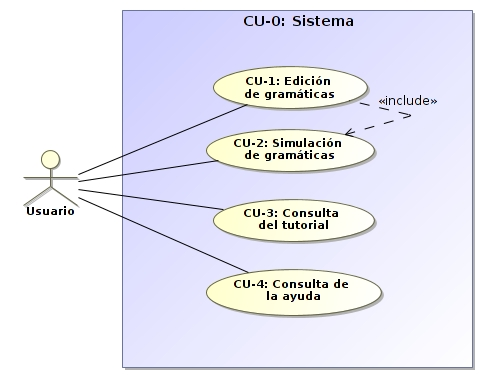
\includegraphics[scale=0.5]{img/CU0.jpg}
	\caption{Diagrama de contexto del Sistema}
	\label{fig:diagramaContexto}
      \end{center}
  \end{figure}

\begin{longtable}[H]{|>{\columncolor[rgb]{0.63,0.79,0.95}}m{6cm} | m{8.5cm} |}
 \caption{Caso de uso: CU-0. Sistema}

\endfirsthead

\multicolumn{2}{c}
{{\tablename\ \thetable{} -- contin�a de la p�gina anterior}} \\
\endhead

\hline \multicolumn{2}{|r|}{{Contin�a en la p�gina siguiente}} \\ \hline
\endfoot

\hline
\endlastfoot

\hline
 \textbf{Nombre} & \textbf{CU-0. Sistema} (diagrama de contexto).\newline \textbf{Nivel}: 0  \\ \hline
 
 \textbf{Descripci�n} &  Tiene como objetivo presentar al usuario todos 
				los subsistemas que componen la aplicaci�n, registr�ndose
                       todas las interacciones que el usuario pueda tener con estos. \\ \hline
                       
 \textbf{Actores} & Usuario \\ \hline
 
 \textbf{Casos de uso} & \begin{enumerate}
                                   \item \textbf{CU-1. Edici�n de gram�ticas}: este subsistema se encarga de 												editar gram�ticas de contexto libre.
                                   \item \textbf{CU-2. Simulaci�n de gram�ticas}: este subsistema tiene como 													objetivo simular gram�ticas de contexto libre.
                                   \item \textbf{CU-3. Consulta del tutorial}: permite consultar el 														tutorial de la aplicaci�n.
                                   \item \textbf{CU-4. Consulta de la ayuda}: este subsistema permite 													consultar la ayuda de la aplicaci�n.
                                 \end{enumerate} \\ \hline
                                 
 \textbf{Flujo de eventos principal} & \begin{enumerate}
                                                 \item El usuario accede al Sistema.
                                                 \item Se muestran todas las opciones disponibles al 														usuario.
                                                 \item El usuario selecciona alguna de las opciones 															del Sistema.
                                               \end{enumerate} \\ \hline
 \textbf{Flujo de eventos alternativo} & \begin{enumerate}
                                               \item Se registra un error durante el proceso de 															inicializaci�n del Sistema.
                                                 \item Se informa al usuario del error producido.
                                                 \item El Sistema finaliza su ejecuci�n.
                                               \end{enumerate} 
 \label{tabla71}

\end{longtable}

A continuaci�n se proceder� a refinar todos los casos de uso que componen la funcionalidad del simulador. Este refinamiento se llevar� a cabo de forma ordenada, para cada caso de uso general (CU-1, CU-2, CU-3 y CU-4) que se identific� en el diagrama de contexto.

\section{Refinamiento de CU-1: Edici�n de gram�ticas}

Este caso de uso representa la edici�n de gram�ticas de contexto libre en el sistema. En la figura 
\ref{fig:CU1_EdicionDeGramatica} se muestra la representaci�n gr�fica de este caso de uso, que est� formada
por los siguientes sub-casos de uso:

\begin{itemize}
 \item \textbf{CU-1.1. Crear gram�tica}.
 \item \textbf{CU-1.2. Editar vocabulario de la gram�tica}.
 \item \textbf{CU-1.3. Editar producci�n}.
 \item \textbf{CU-1.4. Seleccionar el s�mbolo inicial}.
 \item \textbf{CU-1.5. Cerrar gram�tica}.
 \item \textbf{CU-1.6. Recuperar gram�tica}.
 \item \textbf{CU-1.7. Guardar gram�tica}.
 \item \textbf{CU-1.8. Validar gram�tica}.
 \item \textbf{CU-1.9. Generar informe de gram�tica}.
 \item \textbf{CU-1.10. Transferir al simulador}.
 \item \textbf{CU-1.11. Obtener gram�tica}.
 \item \textbf{CU-1.12. Actualizar visualizaci�n de la gram�tica}.
 \item \textbf{CU-1.13. Comprobar producci�n}.
\end{itemize}


 \begin{figure}[H]
      \begin{center} 
	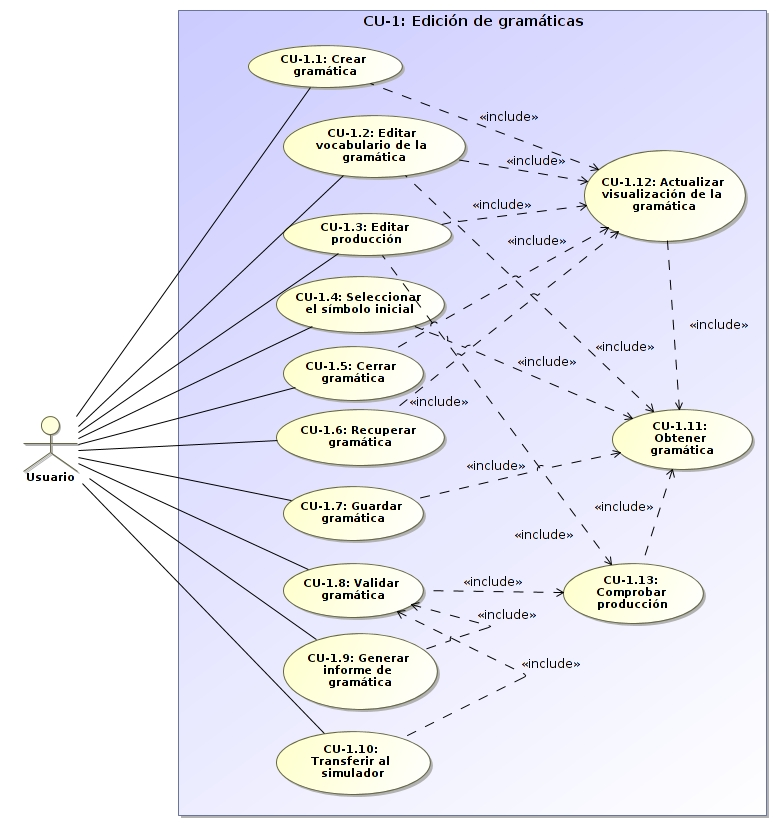
\includegraphics[scale=0.5]{img/CU1.jpg}
	\caption{CU-1: Edicion de gram�ticas}
	\label{fig:CU1_EdicionDeGramatica}
     \end{center}
  \end{figure}

La especificaci�n del caso de uso se muestra en la tabla \ref{tabla72}.


\begin{longtable}[H]{|>{\columncolor[rgb]{0.63,0.79,0.95}}m{6cm} | m{8.5cm} |}

 \caption{Caso de uso: CU-1. Edici�n de gram�ticas}

\endfirsthead

\multicolumn{2}{c}
{{\tablename\ \thetable{} -- contin�a de la p�gina anterior}} \\
\endhead

\hline \multicolumn{2}{|r|}{{Contin�a en la p�gina siguiente}} \\ \hline
\endfoot

\hline
\endlastfoot

\hline
 \textbf{Nombre} & \textbf{CU-1. Edici�n de gram�ticas}. \newline \textbf{Nivel}: 1  \\ \hline
 
 \textbf{Descripci�n} &  Permite al usuario la creaci�n y edici�n de gram�ticas de contexto libre. \\ \hline
                       
 \textbf{Actores} & Usuario \\ \hline
 
 \textbf{Casos de uso} & \begin{enumerate}
				  \item \textbf{CU-1.1. Crear gram�tica}: permite \textit{crear} una gram�tica a partir de 							una producci�n inicial.
				  \item \textbf{CU-1.2. Editar vocabulario de la gram�tica}: permite \textit{editar} el 								vocabulario de s�mbolos ($V_{N}, V_{T}$) de la gram�tica.
				  \item \textbf{CU-1.3. Editar producci�n}: permite la \textit{edici�n} de producciones de la 						gram�tica.
				  \item \textbf{CU-1.4. Seleccionar el s�mbolo inicial}: permite la \textit{selecci�n} del 							s�mbolo inicial de la gram�tica.
				  \item \textbf{CU-1.5. Cerrar gram�tica}: \textit{cierra} una gram�tica abierta en el 								editor.
				  \item \textbf{CU-1.6. Recuperar gram�tica}: \textit{carga} una gram�tica almacenada en un 							fichero.
   				  \item \textbf{CU-1.7. Guardar gram�tica}: \textit{almacena} una gram�tica en un fichero.
				  \end{enumerate} \\
\hline \textbf{Casos de uso} &   \begin{enumerate}  
				  \setcounter{enumi}{7}\item \textbf{CU-1.8. Validar gram�tica}: \textit{va\-li\-da} una 								gram�tica de contexto libre.
				  \item \textbf{CU-1.9. Generar informe}: \textit{ge\-ne\-ra} un informe de una gram�tica de 							contexto libre.
				  \item \textbf{CU-1.10. Transferir al simulador}: \textit{transfiere} 												una gram�tica de contexto libre al simulador para simular el an�lisis sint�ctico.
				  \item \textbf{CU-1.11. Obtener gram�tica}: \textit{obtiene} el vocabulario de s�mbolos 								($V_{N}, V_{T}$) as� como las producciones de la gram�tica.
                  \item \textbf{CU-1.12. Actualizar vi\-sua\-li\-za\-ci�n de la gram�tica}: 											\textit{actualiza} la visualizaci�n de la gram�tica en la interfaz del simulador, 							para permitir al usuario visualizarla a medida que re\-a\-li\-za modificaciones en la 						misma.
                  \item \textbf{CU-1.13. Comprobar producci�n}: \textit{comprueba} si una producci�n es 								correcta o no.
                 
              \end{enumerate}\\ \hline
                                 
 \textbf{Flujo de eventos principal} & \begin{enumerate}
                                                 \item El usuario accede al Sistema.
                                                 \item Se muestran todas las opciones disponibles al 														usuario.
                                                 \item El usuario selecciona alguna de las opciones 															del Sistema.
                                               \end{enumerate} \\ \hline
 \textbf{Flujo de eventos alternativo} & \begin{enumerate}
                                               \item Se registra un error durante el proceso de 															inicializaci�n del Sistema.
                                                 \item Se informa al usuario del error producido.
                                                 \item El Sistema finaliza su ejecuci�n.
                                               \end{enumerate} \\ \hline
                                               
\textbf{Flujo de eventos alternativo} &  La acci�n representada por el caso de uso CU-1.12 se lleva a cabo de forma continuada, sin que lo solicite el usuario. Adem�s, esta acci�n es ejecutada cada vez que el usuario modifica la gram�tica utilizando alguno de los casos de uso que importan este sub-caso de uso. % \hline                                     
 

 \label{tabla72}

\end{longtable}


A continuaci�n, se refinar� cada uno de los casos de uso que componen el caso de uso CU-1.

\subsection{CU-1.1: Crear gram�tica}

Este caso de uso representa la creaci�n de una gram�tica de contexto libre. En la figura
\ref{fig:CU1.1_CrearGramatica} se muestra la representaci�n gr�fica del caso de uso y en la 
tabla \ref{tabla73} se muestra su representaci�n tabular.


\begin{figure}[H]
      \begin{center} 
	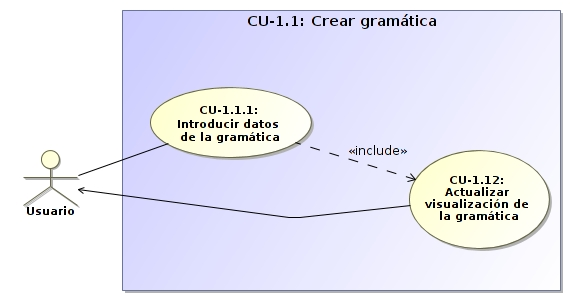
\includegraphics[scale=0.5]{img/CU11.jpg}
	\caption{CU-1.1: Crear gram�tica}
	\label{fig:CU1.1_CrearGramatica}
      \end{center}
  \end{figure}

\begin{longtable}[H]{|>{\columncolor[rgb]{0.63,0.79,0.95}}m{6cm} | m{8.5cm} |}
\caption{Caso de uso: CU-1.1 Crear gram�tica} \\

\endfirsthead

\multicolumn{2}{c}
{{ \tablename\ \thetable{} -- contin�a de la p�gina anterior}} \\
\endhead

\hline \multicolumn{2}{|r|}{{Contin�a en la p�gina siguiente}} \\ \hline
\endfoot

\hline
\endlastfoot


 \hline
 \textbf{Nombre} & \textbf{CU-1.1 Crear gram�tica}.\newline \textbf{Nivel}: 2  \\ \hline
 
 \textbf{Descripci�n} &  Permite al usuario crear 
					  gram�ticas de contexto libre. \\ \hline
                       
 \textbf{Actores} & Usuario \\ \hline
 
 \textbf{Casos de uso} & \begin{enumerate}
				  \item \textbf{CU-1.1.1 Introducir datos de la gram�tica}: permite que el usuario 										\textit{introduzca} los datos de una gram�tica
				  			de contexto libre.
				  \item \textbf{CU-1.12. Actualizar vi\-sua\-li\-za\-ci�n de la gram�tica}: 											\textit{actualiza} la visualizaci�n de la gram�tica en la interfaz del simulador. 
                  \end{enumerate} \\ \hline
                                 
 \textbf{Flujo de eventos principal} & \begin{enumerate}
                  \item El usuario introduce el nombre de la 	gram�tica y una descripci�n de la misma.
                  \item Se crea la gram�tica y se actualiza la visualizaci�n de la interfaz.
                 \end{enumerate} \\ \hline
 \textbf{Flujo de eventos alternativo} & Si en el paso 2 se detecta alg�n e\-rror durante la 					actualizaci�n de la visualizaci�n:
 			\begin{enumerate}
                    \item Se informa al usuario del error producido.
                 \end{enumerate}
 
 
  \label{tabla73}
\end{longtable}

El caso de uso \textit{CU-1.1.1} no es preciso refinarlo m�s, puesto que se trata de un
proceso simple. Este caso de uso se encargar� de pedir el nombre y la descripci�n de la gram�tica (que no s�mbolos y producciones) al usuario para insertarlos en la definici�n de la gram�tica. Estos datos
se encuentran especificados en el cap�tulo anterior.

\subsection{CU-1.2: Editar vocabulario de la gram�tica}

Este caso de uso representa la edici�n del vocabulario de la gram�tica (tanto los s�mbolos terminales como los no terminales). En la figura \ref{fig:CU1.2} se muestra la representaci�n gr�fica del caso de uso y en la tabla \ref{tabla74} se muestra su representaci�n tabular.

 \begin{figure}[H]
      \begin{center} 
	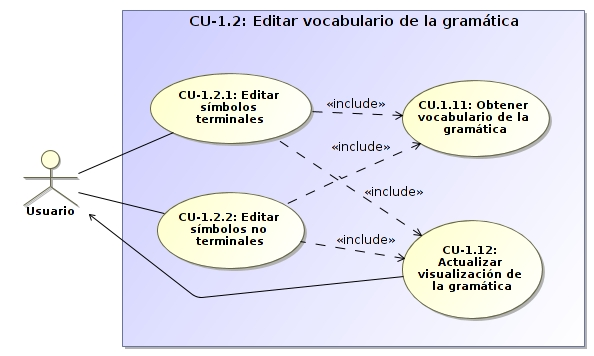
\includegraphics[scale=0.5]{img/CU12.jpg}
	\caption{CU-1.2: Editar vocabulario de la gram�tica}
	\label{fig:CU1.2}
      \end{center}
  \end{figure}

\begin{longtable}[H]{|>{\columncolor[rgb]{0.63,0.79,0.95}}m{6cm} | m{8.5cm} |}
\caption{Caso de uso: CU-1.2 Editar vocabulario de la gram�tica} \\

\endfirsthead

\multicolumn{2}{c}
{{ \tablename\ \thetable{} -- contin�a de la p�gina anterior}} \\
\endhead

\hline \multicolumn{2}{|r|}{{Contin�a en la p�gina siguiente}} \\ \hline
\endfoot

\hline
\endlastfoot


 \hline
 \textbf{Nombre} & \textbf{CU-1.2 Editar vocabulario de la gram�tica}.\newline \textbf{Nivel}: 2  \\ \hline
 
 \textbf{Descripci�n} &  Permite al usuario editar el vocabulario
                                ($V_{N}, V_{T}$) de la gram�tica. \\ \hline
                       
 \textbf{Actores} & Usuario \\ \hline
 
 \textbf{Casos de uso} & \begin{enumerate}
				  \item \textbf{CU-1.2.1 Editar s�mbolos terminales}: permite que el usuario 											\textit{introduzca o modifique} el conjunto de s�mbolos terminales de la 											gram�tica.
				  \item \textbf{CU-1.2.2 Editar s�mbolos no terminales}: permite que el usuario 										\textit{introduzca o modifique} el conjunto de s�mbolos no terminales de la 										gram�tica. 
				  \item \textbf{CU-1.11. Obtener gram�tica}: \textit{obtiene} el vocabulario de s�mbolos 									($V_{N}, V_{T}$) as� como las producciones de la gram�tica.
				  \item \textbf{CU-1.12. Actualizar vi\-sua\-li\-za\-ci�n de la gram�tica}: 												\textit{actualiza} la visualizaci�n de la gram�tica en la interfaz del 										simulador. 									
		                 \end{enumerate} \\ \hline
                                 
 \textbf{Flujo de eventos principal} & \begin{enumerate}
                   \item El usuario elige entre alguna de las opciones disponibles:
                         \begin{enumerate}
						    \item Introducir el conjunto de s�mbolos terminales de la 														gram�tica y se comprueba si son correctos.
                             \item Introducir el conjunto de s�mbolos no terminales de la 													gram�tica y se comprueba si son correctos.     
                           \end{enumerate} 
                     \end{enumerate} \\ \hline
                     
 \textbf{Flujo de eventos alternativo} & Si durante la opci�n o funci�n 1, se detecta que alguno de los 				s�mbolos terminales introducido no es co\-rrec\-to:
 			\begin{enumerate}
                 \item Se informa al usuario del error producido.
                 \item Se pide al usuario que reintroduzca el s�mbolo terminal que produjo el error.
              \end{enumerate}\\ \hline
              
  \textbf{Flujo de eventos alternativo} & Si durante la opci�n o funci�n 2, se detecta que alguno de los 				s�mbolos no 	terminales introducido no es co\-rrec\-to:
  			\begin{enumerate}
                 \item Se informa al usuario del error producido.
              \item Se pide al usuario que reintroduzca el s�mbolo no terminal que produjo el error.
           \end{enumerate}           
 
 
  \label{tabla74}
\end{longtable}

Los casos de uso \textit{CU-1.2.1} y \textit{CU-1.2.2} no se refinar�n m�s, puesto que son casos de uso bastante sencillos y que pueden ser f�cilmente traducidos a una implementaci�n posterior
sin necesidad de ser refinados.

El caso de uso 1.2.1 mostrar�a al usuario una ventana para \textit{introducir} o \textit{modificar} 
(en el caso de que ya los haya introducido) todos los s�mbolos terminales de la gram�tica, 
mientras que el 1.2.2 permitir�a modificar los no terminales.

\subsection{CU-1.3: Editar producci�n}

Este caso de uso representa la edici�n de una producci�n de una gram�tica. En la figura
\ref{fig:CU13} se muestra la representaci�n gr�fica del caso de uso y en la 
tabla \ref{tabla75} se muestra su representaci�n tabular.

  \begin{figure}[H]
      \begin{center} 
	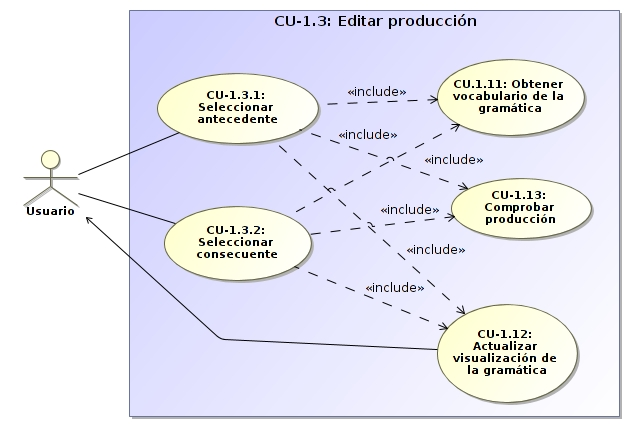
\includegraphics[scale=0.5]{img/CU13.jpg}
	\caption{CU-1.3: Editar producci�n}
	\label{fig:CU13}
      \end{center}
  \end{figure}


\begin{longtable}[H]{|>{\columncolor[rgb]{0.63,0.79,0.95}}m{6cm} | m{8.5cm} |}
\caption{Caso de uso: CU-1.3: Editar producci�n} \\

\endfirsthead

\multicolumn{2}{c}
{{ \tablename\ \thetable{} -- contin�a de la p�gina anterior}} \\
\endhead

\hline \multicolumn{2}{|r|}{{Contin�a en la p�gina siguiente}} \\ \hline
\endfoot

\hline
\endlastfoot


 \hline
 \textbf{Nombre} & \textbf{CU-1.3 Editar producci�n}.\newline \textbf{Nivel}: 2  \\ \hline
 
 \textbf{Descripci�n} & Permite al usuario editar una producci�n de la gram�tica de contexto libre.\\ \hline
                       
 \textbf{Actores} & Usuario \\ \hline
 
 \textbf{Casos de uso} & \begin{enumerate}
				  \item \textbf{CU-1.3.1 Seleccionar antecedente}: permite que el usuario \textit{modifique} 							el antecedente de una producci�n.
				  \item \textbf{CU-1.3.2 Seleccionar consecuente}: permite que el usuario \textit{modifique} 							el consecuente de una producci�n.
				  \item \textbf{CU-1.11. Obtener gram�tica}: \textit{obtiene} el vocabulario de s�mbolos 								($V_{N}, V_{T}$) as� como las producciones de la gram�tica.
				  \item \textbf{CU-1.12. Actualizar vi\-sua\-li\-za\-ci�n de la gram�tica}: 											\textit{actualiza} la visualizaci�n de la gram�tica en la interfaz del simulador.
				  \item \textbf{CU-1.13 Comprobar producci�n}: \textit{comprueba} si una producci�n es 								correcta.
                                 \end{enumerate} \\ \hline
                                 
 \textbf{Flujo de eventos principal} & \begin{enumerate}
                  \item El usuario \textit{selecciona} el antecedente o el consecuente (o 							ambos) de la producci�n que desea crear o modificar (en caso de que en CU-1 el 								usuario hubiera seleccionado alguna producci�n que ya exist�a).
                  \item El usuario \textit{modifica} el antecedente o el consecuente (o ambos).
                  \item Se \textit{comprueba} si la producci�n modificada es correcta.
             \end{enumerate} \\ \hline
                     
 \textbf{Flujo de eventos alternativo} & Si no existe ning�n s�mbolo en el vocabulario de la gram�tica (o 				solamente existe uno de los conjuntos de s�mbolos: terminales o no terminales) o bien alguno de 				los s�mbolos posee un error, se procede como sigue:
 			\begin{enumerate}
                \item Se \textit{informa} al usuario del evento y se le pide que introduzca o modifique el 						conjunto de s�mbolos de la gram�tica.
              \end{enumerate} \\ \hline
              
 \textbf{Flujo de eventos alternativo} & Si se produce alg�n fallo durante el paso 2, se procede como sigue:
			\begin{enumerate}
                 \item Se \textit{informa} al usuario del error producido.
                 \item Se \textit{deshacen} los cambios re\-a\-li\-zados por el usuario en la producci�n.
          \end{enumerate} \\ \hline
 
              
  \textbf{Flujo de eventos alternativo} & Si se comprueba la producci�n resultante y esta no es correcta, se 				procede como sigue:
  			\begin{enumerate}
                  \item Se \textit{informa} al usuario del error (diciendo adem�s si est� en el antecedente, 							en el consecuente o en ambos) y el motivo del mismo.
                  \item Se \textit{pide} al usuario que corrija el e\-rror.
              \end{enumerate}
 
  \label{tabla75}
\end{longtable}

Los casos de uso \textit{CU-1.3.1} y \textit{CU-1.3.2} no se refinar�n m�s, puesto que son casos de uso bastante sencillos y que pueden ser f�cilmente traducidos a una implementaci�n posterior
sin necesidad de ser refinados.

El caso 1.3.1 mostrar�a un di�logo al usuario que le permita seleccionar el antecedente de la producci�n de entre los s�mbolos no terminales que introdujo (mediante el caso de uso 1.2).

El caso de uso 1.3.2, por su parte, permite al usuario modificar el consecuente de la producci�n (re\-a\-li\-zando acciones an�logas a la del caso de uso 1.3.1).

\subsection{CU-1.4: Seleccionar el s�mbolo inicial}

Este caso de uso representa la selecci�n del s�mbolo inicial de la gram�tica. En la figura
\ref{fig:CU14} se muestra la representaci�n gr�fica del caso de uso y en la 
tabla \ref{tabla76} se muestra su representaci�n tabular.

  \begin{figure}[H]
      \begin{center} 
	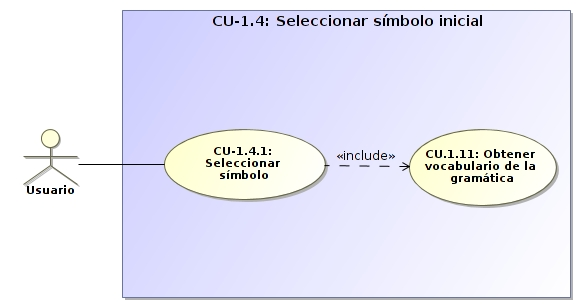
\includegraphics[scale=0.5]{img/CU14.jpg}
	\caption{CU-1.4: Seleccionar el s�mbolo inicial}
	\label{fig:CU14}
      \end{center}
  \end{figure}


\begin{longtable}[H]{|>{\columncolor[rgb]{0.63,0.79,0.95}}m{6cm} | m{8.5cm} |}
\caption{Caso de uso: CU-1.4 Seleccionar el s�mbolo inicial} \\

\endfirsthead

\multicolumn{2}{c}
{{ \tablename\ \thetable{} -- contin�a de la p�gina anterior}} \\
\endhead

\hline \multicolumn{2}{|r|}{{Contin�a en la p�gina siguiente}} \\ \hline
\endfoot

\hline
\endlastfoot


 \hline
 \textbf{Nombre} & \textbf{CU-1.4 Seleccionar el s�mbolo inicial}.\newline \textbf{Nivel}: 2  \\ \hline
 
 \textbf{Descripci�n} & Permite al usuario seleccionar el s�mbolo inicial 
					  de la gram�tica de contexto libre.\\ \hline
                       
 \textbf{Actores} & Usuario \\ \hline
 
 \textbf{Casos de uso} & \begin{enumerate}
				  \item \textbf{CU-1.4.1 Seleccionar s�mbolo}: permite que el usuario \textit{seleccione} un 							s�mbolo inicial de entre el conjunto de s�mbolos no terminales de la 											gram�tica.
				  \item \textbf{CU-1.11. Obtener gram�tica}: \textit{obtiene} el vocabulario de s�mbolos 								($V_{N}, V_{T}$) as� como las producciones de la gram�tica.
                \end{enumerate} \\ \hline
                                 
 \textbf{Flujo de eventos principal} & \begin{enumerate}
                  \item Se \textit{obtienen} los s�mbolos no terminales de la gram�tica.
				  \item Se \textit{muestra} al usuario un di�logo para seleccionar el s�mbolo 								inicial de la gram�tica.
                  \item El usuario \textit{selecciona} un s�mbolo para que sea el inicial.
                  \item Se \textit{comprueba} la producci�n en la que el s�mbolo aparece como antecedente.
                  \item Se \textit{asigna} dicho s�mbolo como s�mbolo inicial.
              \end{enumerate}\\ \hline
                     
 \textbf{Flujo de eventos alternativo} & Si se produce alg�n fallo durante el paso 3, se procede como sigue:
            \begin{enumerate}
                  \item Se \textit{informa} al usuario del error producido.
                  \item Se \textit{termina} la acci�n de seleccionar s�mbolo inicial.
            \end{enumerate}  \\ \hline
              
 \textbf{Flujo de eventos alternativo} & Si se produce alg�n fallo durante el paso 4, se procede como sigue:
            \begin{enumerate}
                  \item Se \textit{informa} al usuario de que la producci�n en la que el s�mbolo aparece en 							el antecedente no es correcta.
                  \item Se \textit{permite} al usuario modificar dicha producci�n.
                  \item Se \textit{reanuda} el paso 4, permitiendo al usuario continuar con la 										asignaci�n de s�mbolo inicial. 
            \end{enumerate} \\ \hline
 
              
  \textbf{Flujo de eventos alternativo} & Si se producen errores en el paso 5, se procede como sigue:
            \begin{enumerate}
                  \item Se \textit{informa} al usuario del error.
                  \item Se \textit{reintenta} asignar el s�mbolo, abortando la acci�n actual en caso de que 							siga siendo imposible dicha asignaci�n.
            \end{enumerate}
 
  \label{tabla76}
\end{longtable}

El caso de uso \textit{CU-1.4.1} no se refinar� m�s, puesto que se trata de un caso de uso bastante sencillo
 y que puede ser f�cilmente traducido a una implementaci�n posterior sin necesidad de ser refinados. Este caso de uso simplemente se encargar�a de mostrar, una vez obtenidos los s�mbolos no terminales de la gram�tica, un di�logo que permita seleccionar el s�mbolo inicial (de entre todos los s�mbolos no terminales que posee la gram�tica).
 
 \subsection{CU-1.5: Cerrar gram�tica}

Este caso de uso se encarga de cerrar la gram�tica seleccionada por el usuario (con una posterior
actualizaci�n de la vista de la gram�tica).

Este caso de uso no se refinar� m�s, puesto que el proceso de cierre de la gram�tica es inmediato y evidente.

\subsection{CU-1.6: Recuperar gram�tica}

Este caso de uso representa la recuperaci�n de una gram�tica desde un fichero. En la figura
\ref{fig:CU16} se muestra la representaci�n gr�fica del caso de uso y en la tabla \ref{tabla77} se muestra
su representaci�n tabular.

 \begin{figure}[H]
      \begin{center} 
	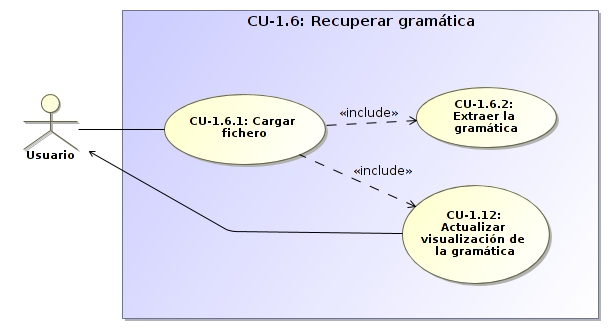
\includegraphics[scale=0.5]{img/CU16.jpg}
	\caption{CU-1.6: Recuperar gram�tica}
	\label{fig:CU16}
      \end{center}
  \end{figure}

\begin{longtable}[H]{|>{\columncolor[rgb]{0.63,0.79,0.95}}m{6cm} | m{8.5cm} |}
\caption{Caso de uso: CU-1.6 Recuperar gram�tica} \\

\endfirsthead

\multicolumn{2}{c}
{{ \tablename\ \thetable{} -- contin�a de la p�gina anterior}} \\
\endhead

\hline \multicolumn{2}{|r|}{{Contin�a en la p�gina siguiente}} \\ \hline
\endfoot

\hline
\endlastfoot


 \hline
 \textbf{Nombre} & \textbf{CU-1.6 Recuperar gram�tica}.\newline \textbf{Nivel}: 2  \\ \hline
 
 \textbf{Descripci�n} & Permite al usuario recuperar una gram�tica de un fichero.\\ \hline
                       
 \textbf{Actores} & Usuario \\ \hline
 
 \textbf{Casos de uso} & \begin{enumerate}
				  \item \textbf{CU-1.6.1 Cargar fichero}: \textit{carga} un fichero que contiene una 								gram�tica.
				  \item \textbf{CU-1.6.2 Extraer la gram�tica}:  \textit{extrae} la gram�tica contenida en el 					fichero recuperado.
				  \item \textbf{CU-1.12. Actualizar visualizaci�n de la gram�tica}: \textit{actualiza} la 						visualizaci�n de la gram�tica en la interfaz del simulador.
                \end{enumerate} \\ \hline
                                 
 \textbf{Flujo de eventos principal} & \begin{enumerate}
                 \item El usuario \textit{selecciona} el fichero que contiene la gram�tica que desea cargar.
                 \item Se \textit{extrae} la gram�tica del fichero.
                 \item Se \textit{carga} la gram�tica en el editor (creando toda la estructura de la 								gram�tica y actualizando la vista de la gram�tica pertinente).
             \end{enumerate}\\ \hline
                     
 \textbf{Flujo de eventos alternativo} & Si se produce alg�n fallo durante el paso 1, se procede como sigue:
              \begin{enumerate}
                 \item Se \textit{informa} al usuario de que no ha podido seleccionar ning�n fichero.
                 \item Se \textit{termina} la acci�n de recuperar gram�tica.
              \end{enumerate}  \\ \hline
              
 \textbf{Flujo de eventos alternativo} & Si se produce alg�n fallo durante el paso 2, se procede como sigue:
              \begin{enumerate}
                  \item Se \textit{informa} al usuario de que la gram�tica no pudo ser extra�da o cargada en 							el simulador, debido a posibles problemas en la estructura del archivo.
                  \item Se \textit{termina} la acci�n de recuperar gram�tica.
            \end{enumerate} \\ \hline
              
  \textbf{Flujo de eventos alternativo} & Si se produce alg�n fallo durante el paso 3, se procede como sigue:
              \begin{enumerate}
                  \item Se \textit{informa} al usuario de que la gram�tica ha podido ser extra�da pero no se 						puede cargar en el editor.
                  \item Se \textit{termina} la acci�n de recuperar gram�tica.
              \end{enumerate}
 
  \label{tabla77}
\end{longtable}

Los casos de uso \textit{CU-1.6.1} y \textit{CU-1.6.2} no se refinar�n m�s, puesto que son casos de uso bastante sencillos y que pueden ser f�cilmente traducidos a una implementaci�n posterior sin necesidad de ser refinados.

\subsection{CU-1.7: Guardar gram�tica}

Este caso de uso representa el guardado de una gram�tica. En la figura \ref{fig:CU17} se muestra la
representaci�n gr�fica del caso de uso y en la tabla \ref{tabla78} se muestra su representaci�n tabular.

  \begin{figure}[H]
      \begin{center} 
	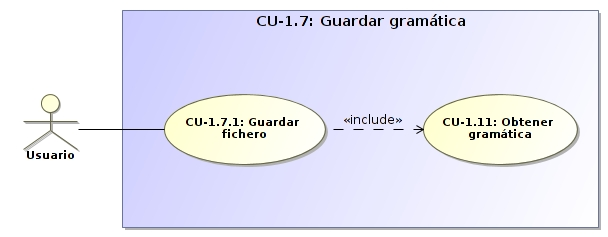
\includegraphics[scale=0.5]{img/CU17.jpg}
	\caption{CU-1.7: Guardar gram�tica}
	\label{fig:CU17}
      \end{center}
  \end{figure}
  
  \newpage

\begin{longtable}[H]{|>{\columncolor[rgb]{0.63,0.79,0.95}}m{6cm} | m{8.5cm} |}
\caption{Caso de uso: CU-1.7 Guardar gram�tica} \\

\endfirsthead

\multicolumn{2}{c}
{{ \tablename\ \thetable{} -- contin�a de la p�gina anterior}} \\
\endhead

\hline \multicolumn{2}{|r|}{{Contin�a en la p�gina siguiente}} \\ \hline
\endfoot

\hline
\endlastfoot


 \hline
 \textbf{Nombre} & \textbf{CU-1.7 Guardar gram�tica}.\newline \textbf{Nivel}: 2  \\ \hline
 
 \textbf{Descripci�n} & Permite al usuario guardar una gram�tica de un fichero.\\ \hline
                       
 \textbf{Actores} & Usuario \\ \hline
 
 \textbf{Casos de uso} & \begin{enumerate}
				  \item \textbf{CU-1.7.1 Guardar fichero}: \textit{guarda} en un fichero la gram�tica creada.
				  \item \textbf{CU-1.11. Obtener gram�tica}: \textit{obtiene} el vocabulario de s�mbolos 								($V_{N}, V_{T}$) as� como las producciones de la gram�tica.
              \end{enumerate} \\ \hline
                                 
 \textbf{Flujo de eventos principal} & \begin{enumerate}
                  \item El usuario \textit{selecciona} el fichero en el que desea guardar la gram�tica.
                  \item Se \textit{guarda} la gram�tica en un fichero (con el formato especificado en el 								cap�tulo anterior).
                 \end{enumerate}\\ \hline
                     
 \textbf{Flujo de eventos alternativo} & Si se produce alg�n fallo durante el paso 1, se procede como sigue:
              \begin{enumerate}
                 \item Se \textit{informa} al usuario de que no ha podido seleccionar crear el fichero.
                 \item Se \textit{termina} la acci�n de guardar gram�tica.
              \end{enumerate}  \\ \hline
              
 \textbf{Flujo de eventos alternativo} & Si se produce alg�n fallo durante el paso 2, se procede como sigue:
              \begin{enumerate}
                 \item Se \textit{informa} al usuario de que la gram�tica no pudo ser guardada.
                 \item Se \textit{termina} la acci�n de guardar gram�tica.
              \end{enumerate} 
 
  \label{tabla78}
\end{longtable}

El caso de uso \textit{CU-1.7.1} no se refinar� m�s, puesto que se trata de un \textbf{proceso simple} y puede ser f�cilmente traducido a una implementaci�n posterior sin necesidad de ser refinado m�s.

\subsection{CU-1.8: Validar gram�tica}

Este caso de uso representa la validaci�n de una gram�tica. En la figura \ref{fig:CU18} se muestra la
representaci�n gr�fica del caso de uso y en la tabla \ref{tabla79} se muestra su representaci�n tabular.

\begin{figure}[H]
      \begin{center} 
	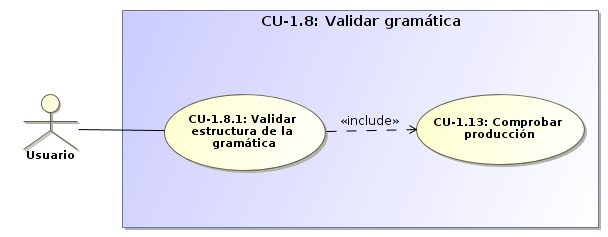
\includegraphics[scale=0.5]{img/CU18.jpg}
	\caption{CU-1.8: Validar gram�tica}
	\label{fig:CU18}
      \end{center}
  \end{figure}
  
  \newpage

\begin{longtable}[H]{|>{\columncolor[rgb]{0.63,0.79,0.95}}m{6cm} | m{8.5cm} |}
\caption{Caso de uso: CU-1.8 Validar gram�tica} \\

\endfirsthead

\multicolumn{2}{c}
{{ \tablename\ \thetable{} -- contin�a de la p�gina anterior}} \\
\endhead

\hline \multicolumn{2}{|r|}{{Contin�a en la p�gina siguiente}} \\ \hline
\endfoot

\hline
\endlastfoot

 \hline
 \textbf{Nombre} & \textbf{CU-1.8 Validar gram�tica}.\newline \textbf{Nivel}: 2  \\ \hline
 
 \textbf{Descripci�n} & Permite al usuario validar una gram�tica de contexto libre.\\ \hline
                       
 \textbf{Actores} & Usuario \\ \hline
 
 \textbf{Casos de uso} & \begin{enumerate}
				  \item \textbf{CU-1.8.1 Validar estructura de la gram�tica}: \textit{valida} la estructura 							de la gram�tica, formada por el conjunto de producciones, s�mbolos 											(\textit{terminales} y \textit{no terminales}) y s�mbolo inicial.
				  \item \textbf{CU-1.12 Comprobar producci�n}: \textit{comprueba} si una producci�n es 								correcta. 
               \end{enumerate} \\ \hline
                                 
 \textbf{Flujo de eventos principal} & \begin{enumerate}
                  \item Se \textit{obtiene} todo el vocabulario de la gram�tica a ser validada. 
                  \item Se \textit{comprueban} todas las producciones que componen la gram�tica.
                  \item Se \textit{informa} al usuario acerca del resultado del la validaci�n.
              \end{enumerate}\\ \hline
                     
 \textbf{Flujo de eventos alternativo} & Si se produce alg�n fallo durante el paso 1, se procede como sigue:
             \begin{enumerate}
                  \item Se \textit{informa} al usuario de que no ha podido obtener el vocabulario de 							la gram�tica.
                  \item Se \textit{termina} la acci�n de validar gram�tica.
             \end{enumerate}  \\ \hline
              
 \textbf{Flujo de eventos alternativo} & Si se produce alg�n fallo durante el paso 2, se procede como sigue:
             \begin{enumerate}
                  \item Se \textit{informa} al usuario de que no se han podido comprobar las producciones de 							la gram�tica.
                  \item Se \textit{termina} la acci�n de validar gram�tica.
             \end{enumerate} \\ \hline
             
 \textbf{Flujo de eventos excepcional} & Si durante la ejecuci�n del paso 2, alguna producci�n comprobada 				posee e\-rro\-res (esto excluye cualquier error de funcionamiento, des\-cri\-to en el flujo 					alternativo anterior), se procede como sigue:
            \begin{enumerate}
                \item El \textit{resultado} de la validaci�n ser� insatisfactorio.
            \end{enumerate}
 
  \label{tabla79}
\end{longtable}

El caso de uso \textit{CU-1.8.1} no se refinar� m�s, puesto que es un proceso simple y que puede
ser f�cilmente traducido a una implementaci�n posterior sin necesidad de ser refinado m�s.

\subsection{CU-1.9: Generar informe de gram�tica}

Este caso de uso representa la generaci�n de un informe de una gram�tica. En la figura
\ref{fig:CU19} se muestra la representaci�n gr�fica del caso de uso y en la 
tabla \ref{tabla710} se muestra su representaci�n tabular.

 \begin{figure}[H]
      \begin{center} 
	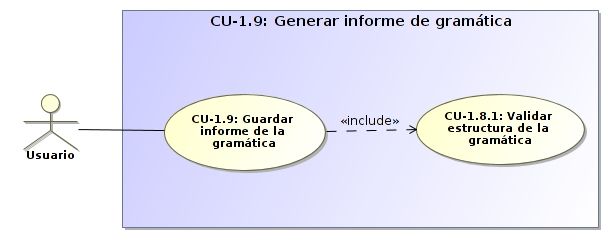
\includegraphics[scale=0.5]{img/CU19.jpg}
	\caption{CU-1.9: Generar informe de gram�tica}
	\label{fig:CU19}
      \end{center}
  \end{figure}

\begin{longtable}[H]{|>{\columncolor[rgb]{0.63,0.79,0.95}}m{6cm} | m{8.5cm} |}
\caption{Caso de uso: CU-1.9 Generar informe de gram�tica} \\

\endfirsthead

\multicolumn{2}{c}
{{ \tablename\ \thetable{} -- contin�a de la p�gina anterior}} \\
\endhead

\hline \multicolumn{2}{|r|}{{Contin�a en la p�gina siguiente}} \\ \hline
\endfoot

\hline
\endlastfoot

 \hline
 \textbf{Nombre} & \textbf{CU-1.9 Generar informe de gram�tica}. \newline \textbf{Nivel}: 2  \\ \hline
 
 \textbf{Descripci�n} & Permite al usuario generar un informe de una gram�tica.\\ \hline
                       
 \textbf{Actores} & Usuario \\ \hline
 
 \textbf{Casos de uso} & \begin{enumerate}
				  \item \textbf{CU-1.9.1 Guardar informe de la gram�tica}: \textit{guarda} un fichero que 							contiene el informe de la gram�tica.
				  \item \textbf{CU-1.8.1 Validar estructura de la gram�tica}: \textit{valida} la estructura 							de la gram�tica, formada por el conjunto de producciones y s�mbolos 											(\textit{terminales} y \textit{no terminales}).
               \end{enumerate} \\ \hline
                                 
 \textbf{Flujo de eventos principal} & \begin{enumerate}
                  \item Se re\-a\-li\-za una \textit{validaci�n} de la estructura de la gram�tica, para as� 							comprobar si la gram�tica es co\-rrec\-ta.
                  \item Se \textit{genera} un informe de la gram�tica, seg�n lo especificado en \textit{RI-							INF-1}.
              \end{enumerate}\\ \hline
                     
 \textbf{Flujo de eventos alternativo} & Si se produce alg�n fallo durante el paso 1, se procede como sigue:
              \begin{enumerate}
                   \item Se \textit{informa} al usuario que no ha podido generar el informe de la 									gram�tica.
                   \item Se \textit{termina} la acci�n de generar informe de gram�tica.
              \end{enumerate}   \\ \hline
              
 \textbf{Flujo de eventos alternativo} & Si se produce alg�n fallo durante el paso 2, se procede como sigue:
               \begin{enumerate}
                   \item Se \textit{informa} al usuario de que el informe no ha podido ser guardado.
                   \item Se \textit{termina} la acci�n de generar informe de gram�tica.
               \end{enumerate}  \\ \hline
             
 \textbf{Flujo de eventos excepcional} & Si durante la ejecuci�n del paso 1, se detecta que la gram�tica no 			es v�lida, puesto que posee errores (esto excluye cualquier error de funcionamiento, descrito en el 			flujo alternativo anterior), se procede como sigue:
               \begin{enumerate}
                   \item Se \textit{aborta} la generaci�n del informe.
                   \item Se \textit{informa} al usuario de que la gram�tica contiene errores.
               \end{enumerate}
 
  \label{tabla710}
\end{longtable}

El caso de uso \textit{CU-1.9.1} no se refinar� m�s, puesto que es un \textbf{proceso simple} y puede
ser f�cilmente traducido a una implementaci�n posterior sin necesidad de ser refinado.

\subsection{CU-1.10: Transferir al simulador}

Este caso de uso representa la transferencia de una gram�tica al simulador. En la figura
\ref{fig:CU110} se muestra la representaci�n gr�fica del caso de uso y en la 
tabla \ref{tabla711} se muestra su representaci�n tabular.

\begin{figure}[H]
      \begin{center} 
	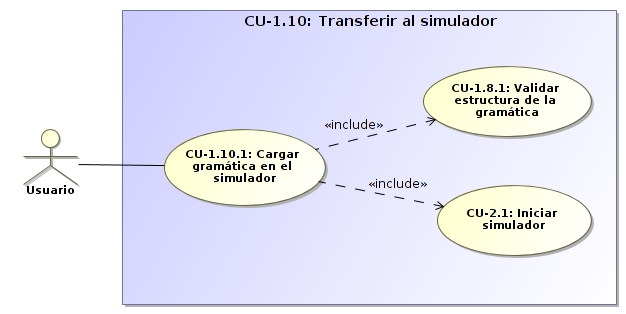
\includegraphics[scale=0.5]{img/CU110.jpg}
	\caption{CU-1.10: Transferir al simulador}
	\label{fig:CU110}
      \end{center}
  \end{figure}

\begin{longtable}[H]{|>{\columncolor[rgb]{0.63,0.79,0.95}}m{6cm} | m{8.5cm} |}
\caption{Caso de uso: CU-1.10 Transferir al simulador} \\

\endfirsthead

\multicolumn{2}{c}
{{ \tablename\ \thetable{} -- contin�a de la p�gina anterior}} \\
\endhead

\hline \multicolumn{2}{|r|}{{Contin�a en la p�gina siguiente}} \\ \hline
\endfoot

\hline
\endlastfoot

 \hline
 \textbf{Nombre} & \textbf{CU-1.10 Transferir al simulador}.\newline \textbf{Nivel}: 2  \\ \hline
 
 \textbf{Descripci�n} & Permite al usuario transferir una gram�tica al simulador para simular un m�todo de 							an�lisis sint�ctico.\\ \hline
                       
 \textbf{Actores} & Usuario \\ \hline
 
 \textbf{Casos de uso} & \begin{enumerate}
				  \item \textbf{CU-1.10.1 Cargar gram�tica en el simulador}: \textit{carga} la gram�tica en 							el si\-mu\-la\-dor.
				  \item \textbf{CU-1.8.1 Validar estructura de la gram�tica}: \textit{valida} la estructura 							de la gram�tica, formada por el conjunto de producciones y s�mbolos 											(\textit{terminales} y \textit{no terminales}).
                  \item \textbf{CU-2.1. Iniciar el simulador}: \textit{i\-ni\-cia\-li\-za} el simulador y 							transfiere la gram�tica, o simplemente carga la gram�tica en el simulador (en el caso 						de que este ya se encuentre ini\-cia\-li\-zado previamente).
               \end{enumerate} \\ \hline
                                 
 \textbf{Flujo de eventos principal} & \begin{enumerate}
                  \item Se \textit{re\-a\-li\-za} una validaci�n de la estructura de la gram�tica, para as� 							comprobar si la gram�tica es co\-rre\-cta.
                  \item Se \textit{transfiere} la gram�tica al si\-mu\-la\-dor y se ini\-cia\-li\-za este (en 						caso de que no se haya iniciado anteriormente al transferir otra gram�tica)
              \end{enumerate}\\ \hline
                     
 \textbf{Flujo de eventos alternativo} & Si se produce alg�n fallo durante el paso 1, se procede como sigue:
              \begin{enumerate}
                  \item Se \textit{informa} al usuario de que no ha podido validar la gram�tica.
                  \item Se \textit{termina} la acci�n de transferir al si\-mu\-la\-dor.
              \end{enumerate}  \\ \hline
              
 \textbf{Flujo de eventos alternativo} & Si se produce alg�n fallo durante el paso 2, se procede como sigue:
              \begin{enumerate}
                  \item Se \textit{informa} al usuario de que no se ha podido transferir la gram�tica
                  \item Se \textit{termina} la acci�n de transferir al si\-mu\-la\-dor.
              \end{enumerate}  \\ \hline
             
 \textbf{Flujo de eventos excepcional} & Si durante la ejecuci�n del paso 1, se detecta que la gram�tica no 				es v�lida, puesto que posee errores (esto excluye cualquier error de funcionamiento, des\-cri\-to 			en el flujo alternativo anterior), se procede como sigue:
              \begin{enumerate}
                  \item Se \textit{aborta} la transferencia de la gram�tica.
                  \item Se \textit{informa} al usuario de que la gram�tica contiene errores (no es una 								gram�tica v�lida).
             \end{enumerate}
 
  \label{tabla711}
\end{longtable}

El caso de uso \textit{CU-1.10.1} no se refinar� m�s, puesto que se trata de un proceso simple, que puede ser f�cilmente traducido a una implementaci�n posterior sin necesidad de ser refinado.

\subsection{CU-1.11: Obtener gram�tica}

Este caso de uso se encarga de obtener el vocabulario de la gram�tica $ (V_{N}, V_{T}) $, as� como todo
el conjunto de producciones y el s�mbolo inicial.

Se trata de un proceso bastante sencillo, pero que es utilizado en los dem�s casos de uso cada vez
que se desea obtener la estructura de una gram�tica. Este caso de uso ser� directamente traducido a una 
implementaci�n sin ser preciso re\-a\-li\-zar un refinamiento m�s exhaustivo.

\subsection{CU-1.12: Actualizar visualizaci�n}

Este caso de uso representa la actualizaci�n de la visualizaci�n de una gram�tica. Cabe destacar que este caso de uso no es invocado directamente por el usuario, sino que el propio Sistema
actualiza la vista de la gram�tica autom�ticamente, a medida que esta sufre alguna modificaci�n (a partir
de aquellos casos de uso que incluyen el comportamiento de este caso de uso). En la figura
\ref{fig:CU112} se muestra la representaci�n gr�fica del caso de uso y en la  tabla \ref{tabla712} se muestra su representaci�n tabular.

 \begin{figure}[H]
      \begin{center} 
	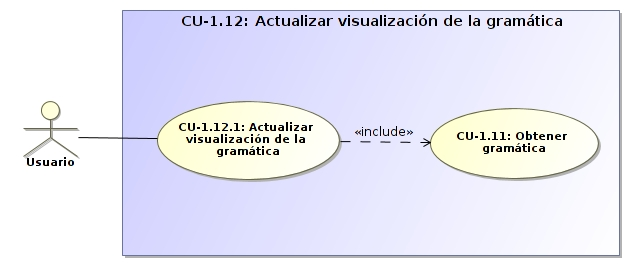
\includegraphics[scale=0.5]{img/CU112.jpg}
	\caption{CU-1.12: Actualizar visualizaci�n de la gram�tica}
	\label{fig:CU112}
      \end{center}
  \end{figure}

\begin{longtable}[H]{|>{\columncolor[rgb]{0.63,0.79,0.95}}m{6cm} | m{8.5cm} |}
\caption{Caso de uso: CU-1.12 Actualizar visualizaci�n de la gram�tica} \\

\endfirsthead

\multicolumn{2}{c}
{{ \tablename\ \thetable{} -- contin�a de la p�gina anterior}} \\
\endhead

\hline \multicolumn{2}{|r|}{{Contin�a en la p�gina siguiente}} \\ \hline
\endfoot

\hline
\endlastfoot

 \hline
 \textbf{Nombre} & \textbf{CU-1.12 Actualizar visualizaci�n de la gram�tica}.\newline \textbf{Nivel}: 2  \\ \hline
 
 \textbf{Descripci�n} & Permite al usuario visualizar la gram�tica a medida que la va construyendo.\\ \hline
                       
 \textbf{Actores} & Usuario \\ \hline
 
 \textbf{Casos de uso} & \begin{enumerate}
				  \item \textbf{CU-1.12.1 Actualizar vi\-sua\-li\-za\-ci�n de la gram�tica}: \textit{ac\-								tua\-li\-za} la vi\-sua\-li\-za\-ci�n de la gram�tica en el editor, a medida que esta 						sufre alguna modificaci�n en su estructura (producciones y s�mbolos).
				  \item \textbf{CU-1.11. Obtener gram�tica}: \textit{obtiene} el vocabulario de s�mbolos 								($V_{N}, V_{T}$) as� como las producciones de la gram�tica.
             \end{enumerate} \\ \hline
                                 
 \textbf{Flujo de eventos principal} & \begin{enumerate}
                  \item Se \textit{obtiene} el vocabulario de la gram�tica.
                  \item Se \textit{actualiza} la vista de la gram�tica en el editor de gram�ticas.
               \end{enumerate}\\ \hline
                     
 \textbf{Flujo de eventos alternativo} & Si se produce alg�n fallo durante el paso 1, se procede como sigue:
              \begin{enumerate}
                  \item Se \textit{informa} al usuario de que no ha podido obtener el vocabulario de la 								gram�tica y que existen errores que impiden vi\-sua\-li\-zar\-la.
                  \item Se \textit{aborta} la actualizaci�n de la vista de la gram�tica.
              \end{enumerate}  \\ \hline
              
 \textbf{Flujo de eventos alternativo} & Si se produce alg�n fallo durante el paso 2, se procede como sigue:
              \begin{enumerate}
                  \item Se \textit{informa} al usuario de que no ha podido actualizar la vista de la 									gram�tica.
                  \item Se \textit{aborta} la actualizaci�n de la vista de la gram�tica.
               \end{enumerate}  
 
  \label{tabla712}
\end{longtable}

El casos de uso \textit{CU-1.12.1} no se refinar� m�s, puesto que se trata de un proceso simple,
que puede ser f�cilmente traducido a una implementaci�n posterior sin necesidad de ser refinado.

\subsection{CU-1.13: Comprobar producci�n}

Este caso de uso se encargar�a de comprobar si la estructura de una producci�n es correcta, seg�n las normas
que se recogen en los anexos de este manual (referente a las producciones de las gram�ticas
de contexto libre).


\section{Refinamiento de CU-2: Simulaci�n de gram�ticas}

Este caso de uso representa la si\-mu\-la\-ci�n del an�lisis sint�ctico tanto ascendente como descendente con una gram�tica de contexto libre. En la figura \ref{fig:CU2} se muestra la representaci�n gr�fica de este caso de uso, que est� formada por los siguientes sub-casos de uso:

\begin{itemize}
 \item \textbf{CU-2.1. Simulador An�lisis Descendente}.
 \item \textbf{CU-2.2. Simulador An�lisis Ascendente}.
 \item \textbf{CU-2.3. Buscar gram�tica}.
\end{itemize}

\begin{figure}[H]
      \begin{center} 
	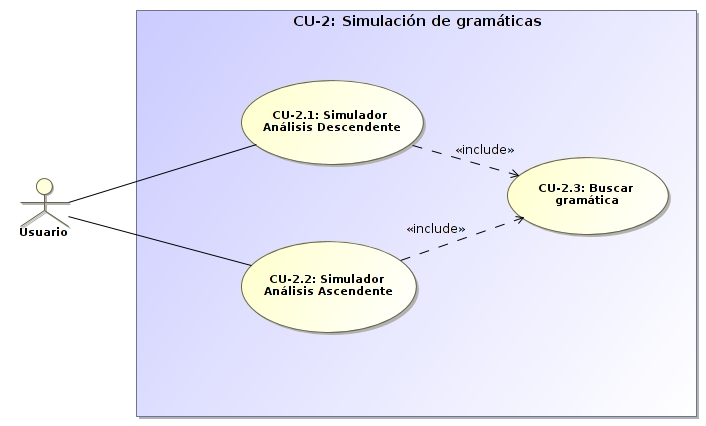
\includegraphics[scale=0.5]{img/CU2.jpg}
	\caption{CU-2: Simulaci�n de gram�ticas}
	\label{fig:CU2}
      \end{center}
  \end{figure}
  
La especificaci�n del caso de uso se muestra en la tabla \ref{tabla715}.


\begin{longtable}[H]{|>{\columncolor[rgb]{0.63,0.79,0.95}}m{6cm} | m{8.5cm} |}
\caption{Caso de uso: CU-2 Simulaci�n de gram�ticas} \\

\endfirsthead

\multicolumn{2}{c}
{{ \tablename\ \thetable{} -- contin�a de la p�gina anterior}} \\
\endhead

\hline \multicolumn{2}{|r|}{{Contin�a en la p�gina siguiente}} \\ \hline
\endfoot

\hline
\endlastfoot

 \hline
 \textbf{Nombre} & \textbf{CU-2. Simulaci�n de de gram�ticas}. \newline \textbf{Nivel}: 1  \\ \hline
 
 \textbf{Descripci�n} & Permite al usuario realizar la simulaci�n de una gram�tica.\\ \hline
                       
 \textbf{Actores} & Usuario \\ \hline
 
 \textbf{Casos de uso} & \begin{enumerate}
				  \item \textbf{CU-2.1 Simulador An�lisis Descendente}: lleva a cabo el an�lisis sint�ctico 						descendente de una gram�tica de contexto libre.
				  
				  \item \textbf{CU-2.2 Simulador An�lisis Ascendente}: lleva a cabo el an�lisis sint�ctico 						ascendente de una gram�tica de contexto libre.
				  
				  \item \textbf{CU-2.3 Buscar gram�tica}: realiza la b�squeda en el sistema de una gram�tica 						de contexto libre guardada con anterioridad.
				  
               \end{enumerate} \\ \hline
                                 
 \textbf{Flujo de eventos principal} & \begin{enumerate}
 				\item Se \textit{selecciona} la gram�tica que se desea simular.
				
				\item Se \textit{elige} entre an�lisis sint�ctico descendente o ascendente.
			\end{enumerate}\\ \hline
                     
 \textbf{Flujo de eventos alternativo} & Si se produce un fallo durante el paso 1, se procede como sigue:
 			\begin{enumerate}
 				\item Se \textit{informa} al usuario que se ha podido cargar la gram�tica seleccionada.
				
                 \item Se \textit{aborta} la selecci�n de la gram�tica y no se podr� llevar a cabo la 							simulaci�n de dicha gram�tica.
                 
                 \item Se redirecciona a la pantalla de simulaci�n.
			\end{enumerate}   
 
  \label{tabla715}
\end{longtable}

A continuaci�n, se refinar� cada uno de los casos de uso que componen el caso de uso CU-2.

\subsection{CU-2.1: Simulaci�n An�lisis descendente}

Este caso de uso representa la simulaci�n del an�lisis sint�ctico descendente de una gram�tica de contexto libre. En la figura \ref{fig:CU21} se muestra la representaci�n gr�fica del caso de uso y en la  tabla \ref{tabla716} se muestra su representaci�n tabular.

 \begin{figure}[H]
      \begin{center} 
	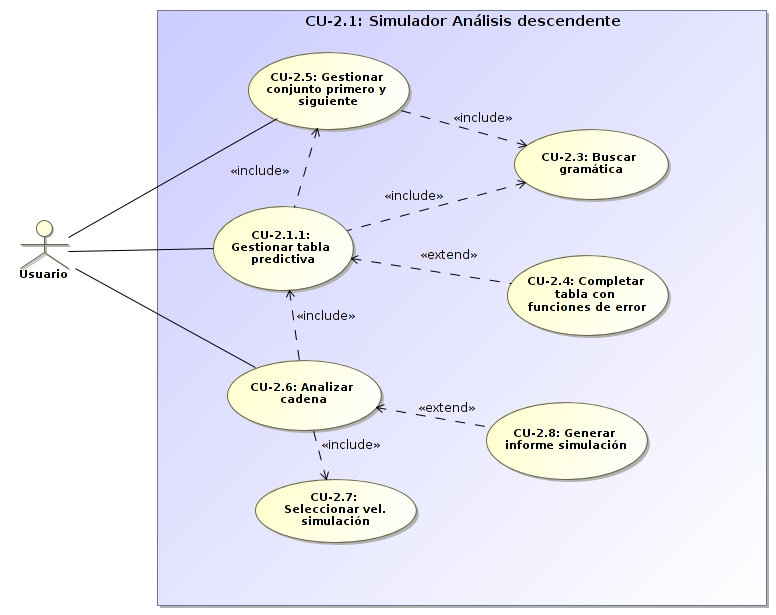
\includegraphics[scale=0.5]{img/CU21.jpg}
	\caption{CU-2.1: Simulaci�n An�lisis descendente}
	\label{fig:CU21}
      \end{center}
  \end{figure}
  
\begin{longtable}[H]{|>{\columncolor[rgb]{0.63,0.79,0.95}}m{6cm} | m{8.5cm} |}
\caption{Caso de uso: CU-2.1 Simulaci�n An�lisis descendente} \\

\endfirsthead

\multicolumn{2}{c}
{{ \tablename\ \thetable{} -- contin�a de la p�gina anterior}} \\
\endhead

\hline \multicolumn{2}{|r|}{{Contin�a en la p�gina siguiente}} \\ \hline
\endfoot

\hline
\endlastfoot

 \hline
 \textbf{Nombre} & \textbf{CU-2.1. Simulaci�n An�lisis descendente}. \newline \textbf{Nivel}: 2  \\ \hline
 
 \textbf{Descripci�n} & Permite al usuario realizar la simulaci�n del an�lisis sint�ctico descendente de una gram�tica de contexto libre.\\ \hline
                       
 \textbf{Actores} & Usuario \\ \hline
 
 \textbf{Casos de uso} & \begin{enumerate}
				  \item \textbf{CU-2.1.1 Gestionar tabla predictiva}: \textit{gestionar} la tabla predictiva 							necesaria para llevar a cabo la simulaci�n.				
				  
				  \item \textbf{CU-2.3 Buscar gram�tica}: realiza la b�squeda en el sistema de una gram�tica 						de contexto libre guardada con anterioridad.
				  
				  \item \textbf{CU-2.4 Completar tabla con funciones de error}: si el usuario lo desea, puede 					\textit{completar} la tabla predictiva con funciones para el tratamiento de los errores 						 que se 	puedan producir.
				  
				  \item \textbf{CU-2.5 Gestionar conjunto primero y siguiente}: \textit{gestionar} el 							conjunto primero y siguiente de una gram�tica de contexto libre, necesarios para crear la 					tabla predictiva.
				  
				  \item \textbf{CU-2.6 Analizar cadena}: \textit{realiza} el an�lisis sint�ctico 									correspondiente de una cadena.
				  
				  \item \textbf{CU-2.7 Seleccionar velocidad de simulaci�n}: \textit{selecciona} la velocidad 					a la que se llevar� a cabo la simulaci�n: paso a paso o continua.
				  
				  \item \textbf{CU-2.8 Generar informe de la simulaci�n}: una vez terminado el proceso de 						simulaci�n, el usuario puede obtener un informe con todos los detalles.
				  
               \end{enumerate} \\ \hline
                                 
 \textbf{Flujo de eventos principal} & \begin{enumerate}
				\item Se \textit{selecciona} la gram�tica que se desea simular.
				
				\item Se \textit{construye} el conjunto primero y siguiente.
				
				\item Se \textit{crea} la tabla predictiva con los datos de los pasos anteriores.
				
				\item Si se desea, se puede \textit{completar} la tabla predictiva con funciones de 								tratamiento de errores.
				
				\item Una vez que se tiene todo lo anterior, se procede a analizar una cadena con el 								simulador.
				
				\item Se \textit{elige} la velocidad de simulaci�n: paso a paso o continua.
				
				\item Se \textit{genera} el informe de la simulaci�n que se ha llevado a cabo en los pasos 						anteriores.
			\end{enumerate}\\ \hline
                     
 \textbf{Flujo de eventos alternativo} & Si se produce un fallo durante el paso 1, se procede como sigue:
 			\begin{enumerate}
				\item Se \textit{informa} al usuario que no se ha podido cargar la gram�tica seleccionada.
				
                 \item Se \textit{aborta} la selecci�n de la gram�tica y no se podr� llevar a cabo la 							simulaci�n.
                 \item Se redirecciona a la pantalla de simulaci�n.
			\end{enumerate}    \\ \hline
			
 \textbf{Flujo de eventos alternativo} & Si se produce un fallo durante el paso 3, se procede como sigue:
 			\begin{enumerate}
				\item Se \textit{informa} al usuario que se ha podido crear la tabla predictiva.
				
                 \item Se \textit{aborta} la creaci�n de la tabla predictiva y no se podr� llevar a cabo 						la simulaci�n hasta que todos los datos sean correctos.
                 
                 \item Se redirecciona a la pantalla de simulaci�n.
			\end{enumerate}   \\ \hline
			
 \textbf{Flujo de eventos alternativo} & Si se produce un fallo durante el paso 5, se procede como sigue:
 			\begin{enumerate}
				\item Se \textit{informa} al usuario que no se ha podido analizar la cadena introducida.
				
                 \item Se \textit{aborta} el an�lisis y no se podr� llevar a cabo hasta que todos los datos 					sean correctos.
                 
                 \item Se redirecciona a la pantalla de simulaci�n.
			\end{enumerate}   \\ \hline
			
 \textbf{Flujo de eventos alternativo} & Si se produce un fallo durante el paso 7, se procede como sigue:
 			\begin{enumerate}
				\item Se \textit{informa} al usuario que no se ha podido generar el informe de la simulaci�n.
				
                 \item Se \textit{aborta} la generaci�n del informe y no se podr� obtener el informe.
                 
                 \item Se redirecciona a la pantalla de simulaci�n.
			\end{enumerate}
 
  \label{tabla716}
\end{longtable}

El casos de uso \textit{CU-2.1} no se refinar� m�s, puesto que se trata de un proceso simple,
que puede ser f�cilmente traducido a una implementaci�n posterior sin necesidad de ser refinado.


\subsection{CU-2.2: Simulaci�n An�lisis ascendente}

Este caso de uso representa la simulaci�n del an�lisis sint�ctico descendente de una gram�tica de contexto libre. En la figura \ref{fig:CU22} se muestra la representaci�n gr�fica del caso de uso y en la  tabla \ref{tabla717} se muestra su representaci�n tabular.


 \begin{figure}[H]
      \begin{center} 
	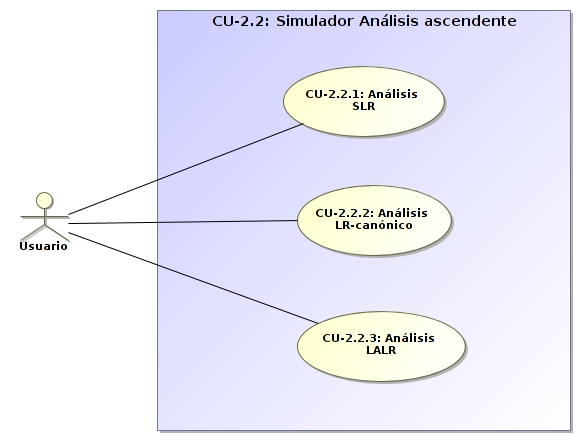
\includegraphics[scale=0.5]{img/CU22.jpg}
	\caption{CU-2.2: Simulaci�n An�lisis ascendente}
	\label{fig:CU22}
      \end{center}
  \end{figure}

\begin{longtable}[H]{|>{\columncolor[rgb]{0.63,0.79,0.95}}m{6cm} | m{8.5cm} |}
\caption{Caso de uso: CU-2.2 Simulaci�n An�lisis ascendente} \\

\endfirsthead

\multicolumn{2}{c}
{{ \tablename\ \thetable{} -- contin�a de la p�gina anterior}} \\
\endhead

\hline \multicolumn{2}{|r|}{{Contin�a en la p�gina siguiente}} \\ \hline
\endfoot

\hline
\endlastfoot

 \hline
 \textbf{Nombre} & \textbf{CU-2.2. Simulaci�n An�lisis ascendente}. \newline \textbf{Nivel}: 2  \\ \hline
 
 \textbf{Descripci�n} & Permite al usuario realizar la simulaci�n del an�lisis sint�ctico ascendente de una gram�tica de contexto libre.\\ \hline
                       
 \textbf{Actores} & Usuario \\ \hline
 
 \textbf{Casos de uso} & \begin{enumerate}
				  \item \textbf{CU-2.2.1 An�lisis SLR}: dentro del an�lisis sint�ctico ascendente realiza el 						an�lisis SLR.
				  
				  \item \textbf{CU-2.2.2 An�lisis LR-can�nico}: dentro del an�lisis sint�ctico ascendente 						realiza el an�lisis LR-can�nico.
				  
				  \item \textbf{CU-2.2.3 An�lisis LALR}: dentro del an�lisis sint�ctico ascendente realiza el 						an�lisis LALR.
				  
               \end{enumerate} \\ \hline
                                 
 \textbf{Flujo de eventos principal} & Si el usuario selecciona una simulaci�n ascendente debe elegir el m�todo de an�lisis: An�lisis SLR, an�lisis, LR-can�nico o an�lisis LALR. \\ \hline
                     
 \textbf{Flujo de eventos alternativo} & Si se produce un error a la hora de seleccionar cualquiera de los m�todos descritos, el simulador informar� al usuario y se podr� continuar con la simulaci�n del an�lisis ascendente. 
 
  \label{tabla717}
\end{longtable}

Posteriormente, se ir� refinando cada uno de los casos de uso contenidos en el \textit{CU-2.2}.


\subsubsection{CU-2.2.1: An�lisis SLR}

Este caso de uso representa el an�lisis SLR dentro del an�lisis sint�ctico ascendente. En la figura \ref{fig:CU221} se muestra la representaci�n gr�fica del caso de uso y en la tabla \ref{tabla7111} se muestra su representaci�n tabular.

\begin{figure}[H]
      \begin{center} 
	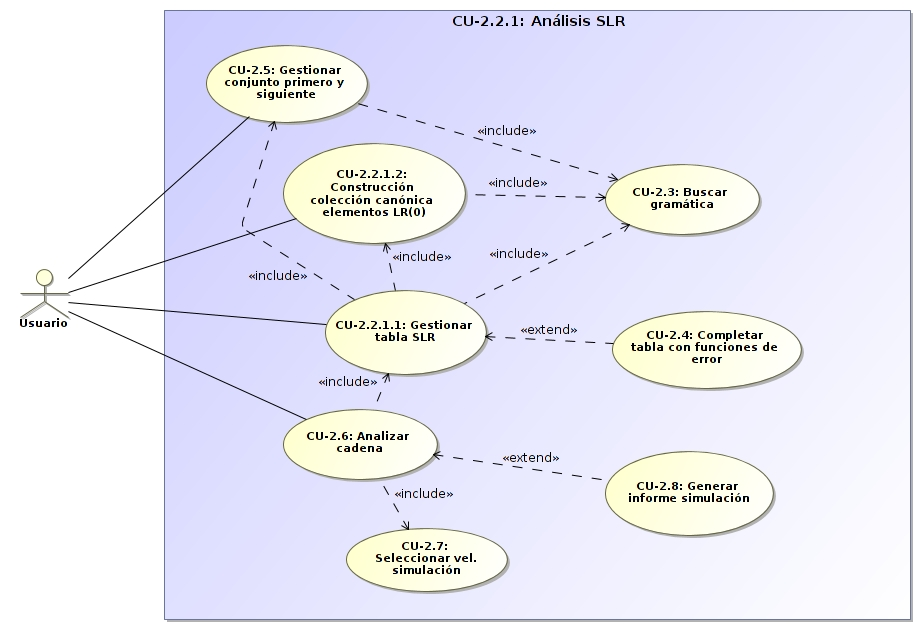
\includegraphics[scale=0.45]{img/CU221.jpg}
	\caption{CU-2.2.1: An�lisis SLR}
	\label{fig:CU221}
      \end{center}
  \end{figure}
  
  \begin{longtable}[H]{|>{\columncolor[rgb]{0.63,0.79,0.95}}m{6cm} | m{8.5cm} |}
\caption{Caso de uso: CU-2.2.1 An�lisis SLR} \\

\endfirsthead

\multicolumn{2}{c}
{{ \tablename\ \thetable{} -- contin�a de la p�gina anterior}} \\
\endhead

\hline \multicolumn{2}{|r|}{{Contin�a en la p�gina siguiente}} \\ \hline
\endfoot

\hline
\endlastfoot

 \hline
 \textbf{Nombre} & \textbf{CU-2.2.1. An�lisis SLR}. \newline \textbf{Nivel}: 3  \\ \hline
 
 \textbf{Descripci�n} & Realiza dentro del an�lisis sint�ctico ascendente, la simulaci�n del m�todo SLR de una gram�tica de contexto libre. \\ \hline
                       
 \textbf{Actores} & Usuario \\ \hline
 
 \textbf{Casos de uso} & \begin{enumerate}
				  \item \textbf{CU-2.2.1.1 Gestionar tabla SLR}: gestionar la tabla SLR necesaria para llevar 					a cabo el an�lisis ascendente.
				  
				  \item \textbf{CU-2.2.1.2 Construcci�n colecci�n can�nica elementos LR(0)}: 	construir la 							colecci�n can�nica de elementos LR(0) necesaria para llevar a cabo el an�lisis 								ascendente SLR.			
				  
				  \item \textbf{CU-2.3 Buscar gram�tica}: realiza la b�squeda en el sistema de una gram�tica 						de contexto libre guardada con anterioridad.
				  
				  \item \textbf{CU-2.4 Completar tabla con funciones de error}: si el usuario lo desea, puede 					\textit{completar} la tabla predictiva con funciones para el tratamiento de los errores 						 que se 	puedan producir.
				  
				  \item \textbf{CU-2.5 Gestionar conjunto primero y siguiente}: \textit{gestionar} el 							conjunto primero y siguiente de una gram�tica de contexto libre, necesarios para crear la 					tabla predictiva.
				  
				  \item \textbf{CU-2.6 Analizar cadena}: \textit{realiza} el an�lisis sint�ctico 									correspondiente de una cadena.
				  
				  \item \textbf{CU-2.7 Seleccionar velocidad de simulaci�n}: \textit{selecciona} la velocidad 					a la que se llevar� a cabo la simulaci�n: paso a paso o continua.
				  
				  \item \textbf{CU-2.8 Generar informe de la simulaci�n}: una vez terminado el proceso de 						simulaci�n, el usuario puede \textit{obtener} un informe con todos los detalles.
				  
               \end{enumerate} \\ \hline
                                 
 \textbf{Flujo de eventos principal} & \begin{enumerate}
				\item Se \textit{selecciona} la gram�tica que se desea simular.
				
				\item Se \textit{construye} el conjunto primero y siguiente.
				
				\item Se \textit{construye} la colecci�n can�nica de elementos LR(0).
				
				\item Se \textit{crea} la tabla SLR con los datos de los pasos anteriores.
				
				\item Si se desea, se puede \textit{completar} la tabla anterior con funciones de 								tratamiento de errores.
				
				\item Una vez que se tiene todo lo anterior, se procede a analizar una cadena con el 								simulador.
				
				\item Se \textit{elige} la velocidad de simulaci�n: paso a paso o continua.
				
				\item Se \textit{genera} el informe de la simulaci�n que se ha llevado a cabo en los pasos 						anteriores.
			\end{enumerate}\\ \hline
                     
 \textbf{Flujo de eventos alternativo} & Si se produce un fallo durante el paso 1, se procede como sigue:
 			\begin{enumerate}
				\item Se \textit{informa} al usuario que se ha podido cargar la gram�tica seleccionada.
				
                 \item Se \textit{aborta} la selecci�n de la gram�tica y no se podr� llevar a cabo la 							simulaci�n.
                 
                 \item Se redirecciona a la pantalla de simulaci�n.
			\end{enumerate}    \\ \hline
			
 \textbf{Flujo de eventos alternativo} & Si se produce un fallo durante el paso 4, se procede como sigue:
 			\begin{enumerate}
				\item Se \textit{informa} al usuario que se ha podido crear la tabla SLR.
				
                 \item Se \textit{aborta} la creaci�n de la tabla SLR y no se podr� llevar a cabo 								la simulaci�n hasta que todos los datos sean correctos.
                 
                 \item Se redirecciona a la pantalla de simulaci�n.
			\end{enumerate}   \\ \hline
			
 \textbf{Flujo de eventos alternativo} & Si se produce un fallo durante el paso 6, se procede como sigue:
 			\begin{enumerate}
				\item Se \textit{informa} al usuario que no se ha podido analizar la cadena introducida.
				
                 \item Se \textit{aborta} el an�lisis y no se podr� llevar a cabo hasta que todos los datos 					sean correctos.
                 
                 \item Se redirecciona a la pantalla de simulaci�n.
			\end{enumerate}   \\ \hline
			
 \textbf{Flujo de eventos alternativo} & Si se produce un fallo durante el paso 8, se procede como sigue:
 			\begin{enumerate}
				\item Se \textit{informa} al usuario que no se ha podido generar el informe de la simulaci�n.
				
                 \item Se \textit{aborta} la generaci�n del informe y no se podr� obtener el informe.
                 
                 \item Se redirecciona a la pantalla de simulaci�n.
			\end{enumerate}
 
  \label{tabla7111}
\end{longtable}

El casos de uso \textit{CU-2.2.1} no se refinar� m�s, puesto que se trata de un proceso simple,
que puede ser f�cilmente traducido a una implementaci�n posterior sin necesidad de ser refinado.


\subsubsection{CU-2.2.2: An�lisis LR-can�nico}

Este caso de uso representa el an�lisis LR-can�nico dentro del an�lisis sint�ctico ascendente. En la figura \ref{fig:CU222} se muestra la representaci�n gr�fica del caso de uso y en la tabla \ref{tabla7112} se muestra su representaci�n tabular.

\begin{figure}[H]
      \begin{center} 
	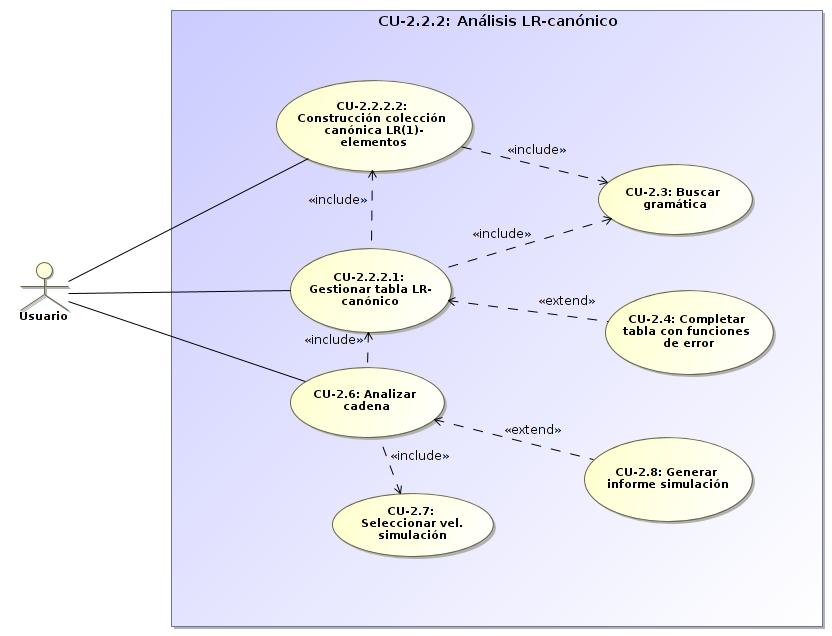
\includegraphics[scale=0.5]{img/CU222.jpg}
	\caption{CU-2.2.1: An�lisis LR-can�nico}
	\label{fig:CU222}
      \end{center}
  \end{figure}
  
  \begin{longtable}[H]{|>{\columncolor[rgb]{0.63,0.79,0.95}}m{6cm} | m{8.5cm} |}
\caption{Caso de uso: CU-2.2.2 An�lisis LR-can�nico} \\

\endfirsthead

\multicolumn{2}{c}
{{ \tablename\ \thetable{} -- contin�a de la p�gina anterior}} \\
\endhead

\hline \multicolumn{2}{|r|}{{Contin�a en la p�gina siguiente}} \\ \hline
\endfoot

\hline
\endlastfoot

 \hline
 \textbf{Nombre} & \textbf{CU-2.2.2. An�lisis LR-can�nico}. \newline \textbf{Nivel}: 3  \\ \hline
 
 \textbf{Descripci�n} & Realiza dentro del an�lisis sint�ctico ascendente, la simulaci�n del m�todo LR-can�nico de una gram�tica de contexto libre.\\ \hline
                       
 \textbf{Actores} & Usuario \\ \hline
 
 \textbf{Casos de uso} &  \begin{enumerate}
				  \item \textbf{CU-2.2.2.1 Gestionar tabla LR-can�nica}: gestionar la tabla LR-can�nica 							necesaria para llevar a cabo el an�lisis ascendente.
				  
				  \item \textbf{CU-2.2.2.2 Construcci�n colecci�n can�nica elementos LR(1)}: 	construir la 							colecci�n can�nica de elementos LR(1) necesaria para llevar a cabo el an�lisis 								ascendente LR-can�nica.			
				  
				  \item \textbf{CU-2.3 Buscar gram�tica}: realiza la b�squeda en el sistema de una gram�tica 						de contexto libre guardada con anterioridad.
				  
				  \item \textbf{CU-2.4 Completar tabla con funciones de error}: si el usuario lo desea, puede 					\textit{completar} la tabla LR-can�nica con funciones para el tratamiento de los errores 						 que se 	puedan producir.
				  
				  \item \textbf{CU-2.6 Analizar cadena}: \textit{realiza} el an�lisis sint�ctico 									correspondiente de una cadena.
				  
				  \item \textbf{CU-2.7 Seleccionar velocidad de simulaci�n}: \textit{selecciona} la velocidad 					a la que se llevar� a cabo la simulaci�n: paso a paso o continua.
				  
				  \item \textbf{CU-2.8 Generar informe de la simulaci�n}: una vez terminado el proceso de 						simulaci�n, el usuario puede \textit{obtener} un informe con todos los detalles.
				  
               \end{enumerate}\\ \hline
                                 
 \textbf{Flujo de eventos principal} & \begin{enumerate}
				\item Se \textit{selecciona} la gram�tica que se desea simular.
				
				\item Se \textit{construye} la colecci�n can�nica de elementos LR(1).
				
				\item Se \textit{crea} la tabla LR-can�nica con los datos de los pasos anteriores.
				
				\item Si se desea, se puede \textit{completar} la tabla anterior con funciones de 								tratamiento de errores.
				
				\item Una vez que se tiene todo lo anterior, se procede a analizar una cadena con el 								simulador.
				
				\item Se \textit{elige} la velocidad de simulaci�n: paso a paso o continua.
				
				\item Se \textit{genera} el informe de la simulaci�n que se ha llevado a cabo en los pasos 						anteriores.
			\end{enumerate}\\ \hline
                     
 \textbf{Flujo de eventos alternativo} & Si se produce un fallo durante el paso 1, se procede como sigue:
 			\begin{enumerate}
				\item Se \textit{informa} al usuario que se ha podido cargar la gram�tica seleccionada.
				
                 \item Se \textit{aborta} la selecci�n de la gram�tica y no se podr� llevar a cabo la 							simulaci�n.
                 
                 \item Se redirecciona a la pantalla de simulaci�n.
			\end{enumerate}    \\ \hline
			
 \textbf{Flujo de eventos alternativo} & Si se produce un fallo durante el paso 3, se procede como sigue:
 			\begin{enumerate}
				\item Se \textit{informa} al usuario que se ha podido crear la tabla LR-can�nica.
				
                 \item Se \textit{aborta} la creaci�n de la tabla y no se podr� llevar a cabo 								la simulaci�n hasta que todos los datos sean correctos.
                 
                 \item Se redirecciona a la pantalla de simulaci�n.
			\end{enumerate}   \\ \hline
			
 \textbf{Flujo de eventos alternativo} & Si se produce un fallo durante el paso 5, se procede como sigue:
 			\begin{enumerate}
				\item Se \textit{informa} al usuario que no se ha podido analizar la cadena introducida.
				
                 \item Se \textit{aborta} el an�lisis y no se podr� llevar a cabo hasta que todos los datos 					sean correctos.
                 
                 \item Se redirecciona a la pantalla de simulaci�n.
			\end{enumerate}   \\ \hline
			
 \textbf{Flujo de eventos alternativo} & Si se produce un fallo durante el paso 7, se procede como sigue:
 			\begin{enumerate}
				\item Se \textit{informa} al usuario que no se ha podido generar el informe de la simulaci�n.
				
                 \item Se \textit{aborta} la generaci�n del informe y no se podr� obtener el informe.
                 
                 \item Se redirecciona a la pantalla de simulaci�n.
			\end{enumerate} 
 
  \label{tabla7112}
\end{longtable}

El casos de uso \textit{CU-2.2.2} no se refinar� m�s, puesto que se trata de un proceso simple,
que puede ser f�cilmente traducido a una implementaci�n posterior sin necesidad de ser refinado.


\subsubsection{CU-2.2.3: An�lisis LALR}

Este caso de uso representa el an�lisis LALR dentro del an�lisis sint�ctico ascendente. En la figura \ref{fig:CU223} se muestra la representaci�n gr�fica del caso de uso y en la tabla \ref{tabla7113} se muestra su representaci�n tabular.

\begin{figure}[H]
      \begin{center} 
	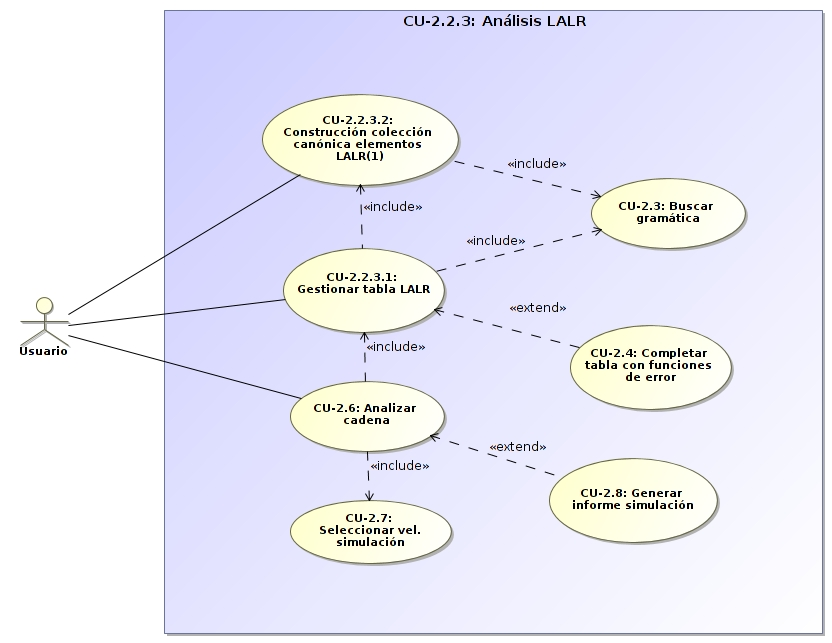
\includegraphics[scale=0.5]{img/CU223.jpg}
	\caption{CU-2.2.1: An�lisis LALR}
	\label{fig:CU223}
      \end{center}
  \end{figure}
  
  \begin{longtable}[H]{|>{\columncolor[rgb]{0.63,0.79,0.95}}m{6cm} | m{8.5cm} |}
\caption{Caso de uso: CU-2.2.3 An�lisis LALR} \\

\endfirsthead

\multicolumn{2}{c}
{{ \tablename\ \thetable{} -- contin�a de la p�gina anterior}} \\
\endhead

\hline \multicolumn{2}{|r|}{{Contin�a en la p�gina siguiente}} \\ \hline
\endfoot

\hline
\endlastfoot

 \hline
 \textbf{Nombre} & \textbf{CU-2.2.3. An�lisis LALR}. \newline \textbf{Nivel}: 3  \\ \hline
 
 \textbf{Descripci�n} & Realiza dentro del an�lisis sint�ctico ascendente, la simulaci�n del m�todo LALR de una gram�tica de contexto libre.\\ \hline
                       
 \textbf{Actores} & Usuario \\ \hline
 
 \textbf{Casos de uso} &  \begin{enumerate}
				  \item \textbf{CU-2.2.3.1 Gestionar tabla LALR}: gestionar la tabla LALR 										necesaria para llevar a cabo el an�lisis ascendente.
				  
				  \item \textbf{CU-2.2.3.2 Construcci�n colecci�n can�nica elementos LR(1)}: 	construir la 							colecci�n can�nica de elementos LR(1) necesaria para llevar a cabo el an�lisis 								ascendente LALR.			
				  
				  \item \textbf{CU-2.3 Buscar gram�tica}: realiza la b�squeda en el sistema de una gram�tica 						de contexto libre guardada con anterioridad.
				  
				  \item \textbf{CU-2.4 Completar tabla con funciones de error}: si el usuario lo desea, puede 					\textit{completar} la tabla LALR con funciones para el tratamiento de los errores 						 que se 	puedan producir.
				  
				  \item \textbf{CU-2.6 Analizar cadena}: \textit{realiza} el an�lisis sint�ctico 									correspondiente de una cadena.
				  
				  \item \textbf{CU-2.7 Seleccionar velocidad de simulaci�n}: \textit{selecciona} la velocidad 					a la que se llevar� a cabo la simulaci�n: paso a paso o continua.
				  
				  \item \textbf{CU-2.8 Generar informe de la simulaci�n}: una vez terminado el proceso de 						simulaci�n, el usuario puede \textit{obtener} un informe con todos los detalles.
				  
               \end{enumerate}\\ \hline
                                 
 \textbf{Flujo de eventos principal} & \begin{enumerate}
				\item Se \textit{selecciona} la gram�tica que se desea simular.
				
				\item Se \textit{construye} la colecci�n can�nica de elementos LR(1).
				
				\item Se \textit{crea} la tabla LALR con los datos de los pasos anteriores.
				
				\item Si se desea, se puede \textit{completar} la tabla anterior con funciones de 								tratamiento de errores.
				
				\item Una vez que se tiene todo lo anterior, se procede a analizar una cadena con el 								simulador.
				
				\item Se \textit{elige} la velocidad de simulaci�n: paso a paso o continua.
				
				\item Se \textit{genera} el informe de la simulaci�n que se ha llevado a cabo en los pasos 						anteriores.
			\end{enumerate}\\ \hline
                     
 \textbf{Flujo de eventos alternativo} & Si se produce un fallo durante el paso 1, se procede como sigue:
 			\begin{enumerate}
				\item Se \textit{informa} al usuario que se ha podido cargar la gram�tica seleccionada.
				
                 \item Se \textit{aborta} la selecci�n de la gram�tica y no se podr� llevar a cabo la 							simulaci�n.
                 
                 \item Se redirecciona a la pantalla de simulaci�n.
			\end{enumerate}    \\ \hline
			
 \textbf{Flujo de eventos alternativo} & Si se produce un fallo durante el paso 3, se procede como sigue:
 			\begin{enumerate}
				\item Se \textit{informa} al usuario que se ha podido crear la tabla LALR.
				
                 \item Se \textit{aborta} la creaci�n de la tabla y no se podr� llevar a cabo 								la simulaci�n hasta que todos los datos sean correctos.
                 
                 \item Se redirecciona a la pantalla de simulaci�n.
			\end{enumerate}   \\ \hline
			
 \textbf{Flujo de eventos alternativo} & Si se produce un fallo durante el paso 5, se procede como sigue:
 			\begin{enumerate}
				\item Se \textit{informa} al usuario que no se ha podido analizar la cadena introducida.
				
                 \item Se \textit{aborta} el an�lisis y no se podr� llevar a cabo hasta que todos los datos 					sean correctos.
                 
                 \item Se redirecciona a la pantalla de simulaci�n.
			\end{enumerate}   \\ \hline
			
 \textbf{Flujo de eventos alternativo} & Si se produce un fallo durante el paso 7, se procede como sigue:
 			\begin{enumerate}
				\item Se \textit{informa} al usuario que no se ha podido generar el informe de la simulaci�n.
				
                 \item Se \textit{aborta} la generaci�n del informe y no se podr� obtener el informe.
                 
                 \item Se redirecciona a la pantalla de simulaci�n.
			\end{enumerate} 
 
  \label{tabla7113}
\end{longtable}

El casos de uso \textit{CU-2.2.3} no se refinar� m�s, puesto que se trata de un proceso simple,
que puede ser f�cilmente traducido a una implementaci�n posterior sin necesidad de ser refinado.


\subsection{CU-2.3: Buscar gram�tica}

Este caso de uso es un proceso simple que consiste en seleccionar una gram�tica de entre las que se encuentran cargadas en el simulador. Por tanto, este proceso no ser� refinado de forma m�s exhaustiva.


\subsection{CU-2.4: Completar tabla con funciones de error}

Este caso de uso es un proceso simple en el cual, una vez construida la tabla del an�lisis sint�ctico, se completa con la funciones de error. Por tanto, este proceso no ser� refinado de forma m�s exhaustiva.

\subsection{CU-2.5: Crear conjunto Primero y siguiente}

Este caso de uso es un proceso simple que consiste en crear los conjuntos primero y siguiente de la gram�tica, necesarios para crear las tablas de an�lisis en el an�lisis sint�ctico descendente y en el an�lisis SLR dentro del an�lisis sint�ctico ascendente. Por tanto, este proceso no ser� refinado de forma m�s exhaustiva.

\subsection{CU-2.6: Analizar cadena}

Este caso de uso es un proceso simple en el cual, se lleva a cabo el an�lisis de una cadena. Por tanto, este proceso no ser� refinado de forma m�s exhaustiva.

\subsection{CU-2.7: Selecciona velocidad de simulaci�n}

Este caso de uso es un proceso simple que consiste en seleccionar entre los dos tipos de velocidad de simulaci�n: paso a paso o continuo. Por tanto, este proceso no ser� refinado de forma m�s exhaustiva.

\subsection{CU-2.8: Generar informe de simulaci�n}

Este caso de uso es un proceso simple que consiste en generar un informe con todos los datos del an�lisis sint�ctico creados durante la simulaci�n, el cual podr� ver y descargar el usuario. Por tanto, este proceso no ser� refinado de forma m�s exhaustiva.


\section{Refinamiento de CU-3: Consulta del tutorial}

Este caso de uso representa la consulta del tutorial de la aplicaci�n. En la figura \ref{fig:CU3} se muestra la representaci�n gr�fica de este caso de uso, que est� formada por los siguientes sub-casos de uso:

\begin{itemize}
 \item \textbf{CU-3.1. Consultar una lecci�n}.
 \item \textbf{CU-3.2. Obtener recurso del tutorial}.
 \item \textbf{CU-3.3. Navegar por el recurso seleccionado}.

\end{itemize}

En este caso de uso se muestran flechas que se dirige desde un caso de uso al usuario. Esto representa el hecho de que el usuario visualiza el tutorial por pantalla.

 \begin{figure}[H]
      \begin{center} 
	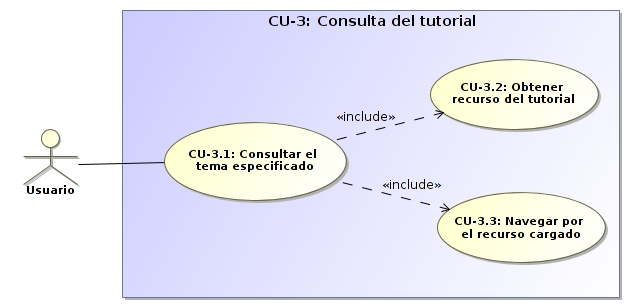
\includegraphics[scale=0.5]{img/CU3.jpg}
	\caption{CU-3: Consulta del tutorial}
	\label{fig:CU3}
      \end{center}
  \end{figure}

La especificaci�n del caso de uso se muestra en la tabla \ref{tabla713}.

  \newpage

\begin{longtable}[H]{|>{\columncolor[rgb]{0.63,0.79,0.95}}m{6cm} | m{8.5cm} |}
\caption{Caso de uso: CU-3. Consulta del tutorial} \\

\endfirsthead

\multicolumn{2}{c}
{{ \tablename\ \thetable{} -- contin�a de la p�gina anterior}} \\
\endhead

\hline \multicolumn{2}{|r|}{{Contin�a en la p�gina siguiente}} \\ \hline
\endfoot

\hline
\endlastfoot

 \hline
 \textbf{Nombre} & \textbf{CU-3. Consulta del tutorial}.\newline \textbf{Nivel}: 1  \\ \hline
 
 \textbf{Descripci�n} & Permite al usuario consultar el tutorial de la aplicaci�n.\\ \hline
                       
 \textbf{Actores} & Usuario \\ \hline
 
 \textbf{Casos de uso} & \begin{enumerate}
 			\item \textbf{CU-3.1. Consultar una lecci�n}: permite \textit{consultar} una lecci�n del 							tutorial.
 			\item \textbf{CU-3.2. Obtener recurso del tutorial}: permite \textit{obtener} una lecci�n del 					tutorial. 
			\item \textbf{CU-3.3. Navegar por el recurso seleccionado}: permite \textit{navegar} por una 						lecci�n del tutorial.
	   \end{enumerate} \\ \hline
                                 
 \textbf{Flujo de eventos principal} & \begin{enumerate}
	         \item Se \textit{obtiene} un recurso del tutorial (especificado por el usuario).
             \item El usuario \textit{navega} por el recurso.
             \item El usuario \textit{accede} a otro recurso a trav�s del enlace (para lo que se vuelve al 					paso 1), o sigue navegando por el mismo.
          \end{enumerate}\\ \hline
                     
 \textbf{Flujo de eventos alternativo} & Si se produce alg�n error al \textit{cargar} o \textit{navegar} por 			un recurso del tutorial, se informa al usuario y se restablece el recurso previo (cerrando el 				tutorial en caso de que se produzca un fallo).
 
  \label{tabla713}
\end{longtable}

N�tese que lo que aqu� se llama recurso del tutorial, es realmente una \textit{lecci�n} del tutorial. El hecho de de\-no\-mi\-nar\-lo recurso implica que el fichero en cuesti�n (un recurso del simulador) es buscado
y cargado, y por tanto, contiene una lecci�n del tutorial.

\section{Refinamiento de CU-4: Consulta de la ayuda}

Este caso de uso representa la consulta de la ayuda de la aplicaci�n. En la figura \ref{fig:CU4} se muestra la representaci�n gr�fica de este caso de uso, que est� formada por los siguientes sub-casos de uso:

\begin{itemize}
 \item \textbf{CU-4.1. Consultar un cap�tulo}.
 \item \textbf{CU-4.2. Obtener recurso de la ayuda}.
 \item \textbf{CU-4.3. Navegar por el recurso seleccionado}.
\end{itemize}

En este caso de uso se muestran flechas que se dirige desde un caso de uso al usuario. Esto representa el hecho de que el usuario visualiza la ayuda por pantalla.

\begin{figure}[H]
      \begin{center} 
	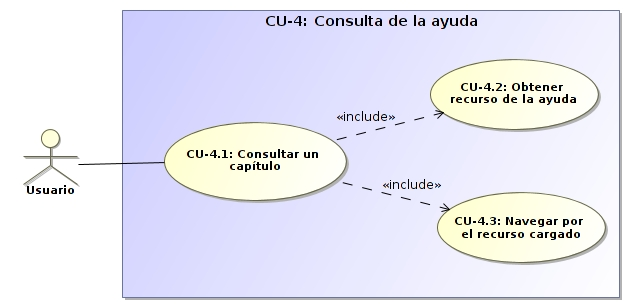
\includegraphics[scale=0.5]{img/CU4.jpg}
	\caption{CU-4: Consulta de la ayuda}
	\label{fig:CU4}
      \end{center}
  \end{figure}

La especificaci�n del caso de uso se muestra en la tabla \ref{tabla714}.

\begin{longtable}[H]{|>{\columncolor[rgb]{0.63,0.79,0.95}}m{6cm} | m{8.5cm} |}
\caption{Caso de uso: CU-4. Consulta de la ayuda} \\

\endfirsthead

\multicolumn{2}{c}
{{ \tablename\ \thetable{} -- contin�a de la p�gina anterior}} \\
\endhead

\hline \multicolumn{2}{|r|}{{Contin�a en la p�gina siguiente}} \\ \hline
\endfoot

\hline
\endlastfoot

 \hline
 \textbf{Nombre} & \textbf{CU-4. Consulta de la ayuda}. \newline \textbf{Nivel}: 1  \\ \hline
 
 \textbf{Descripci�n} & Permite al usuario consultar la ayuda de la aplicaci�n.\\ \hline
                       
 \textbf{Actores} & Usuario \\ \hline
 
 \textbf{Casos de uso} & \begin{enumerate}
 			\item \textbf{CU-4.1. Consultar un cap�tulo}: permite \textit{consultar} un cap�tulo de la ayuda.
 			\item \textbf{CU-4.2. Obtener recurso de la ayuda}: permite \textit{obtener} un cap�tulo de la 					ayuda.
 			\item \textbf{CU-4.3. Navegar por el recurso seleccionado}: permite \textit{navegar} por un 						cap�tulo de la ayuda.
		 \end{enumerate} \\ \hline
                                 
 \textbf{Flujo de eventos principal} & \begin{enumerate}
	        \item Se \textit{obtiene} un recurso de la ayuda (especificado por el usuario).
            \item El usuario \textit{navega} por el recurso.
            \item El usuario \textit{accede} a otro recurso a trav�s del enlace (para lo que se vuelve al 						paso 1), o sigue navegando por el mismo.
          \end{enumerate}\\ \hline
                     
 \textbf{Flujo de eventos alternativo} & Si se produce alg�n error al \textit{cargar} o \textit{navegar} por 			un recurso de la ayuda, se informa al usuario y se restablece el recurso previo (cerrando la ayuda en 		caso de que se produzca un fallo).
              
  \label{tabla714}
\end{longtable}

N�tese que lo que aqu� se llama recurso de la ayuda (al igual que sucedi� con el tutorial), es realmente un \textit{cap�tulo} de la ayuda. El hecho de de\-no\-mi\-nar\-lo recurso implica que el fichero
en cuesti�n (un recurso del simulador) es buscado y cargado, y por tanto, contiene un cap�tulo de la ayuda.


\section{Validaci�n de los casos de uso }

En esta secci�n se realizar� una validaci�n de los casos de uso especificados anteriormente frente a los requisitos de usuario y funcionales del sistema, especificados en el cap�tulo anterior. 

Para mostrar de forma m�s clara y f�cil de entender la validaci�n, esta se llevar� a cabo mediante una tabla en la que se confrontar�n los requisitos funcionales frente a los casos de uso.

\subsection{Validaci�n de los bloques funcionales}

La primera validaci�n que se realizar�, ser� la validaci�n de los bloques funcionales de la aplicaci�n, respecto a los requisitos de usuario del sistema. El resultado de esta validaci�n se recoge en la tabla \ref{val1}.

\begin{table}[H]
\begin{center}

 \caption{Matriz de correspondencia RU-Casos de uso}
 
\resizebox{5.5cm}{!} {
\begin{tabular}[c]{| c | c | c | c | c | c | }
\hline

  \multicolumn{6}{|c|}{\textbf{Casos de uso}} \\ \hline
  \multirow{6}{0.3cm}{\begin{sideways}\textbf{Requisitos de usuario \ \ \ \ \ \ \ \ \ \ \ \ \ \ \ \ \ \ \ \ \ \ \ \ \ \ \ \ \ \ \ \ \ \ \ \ \ \ \ \ \ \ \ \ \ }\end{sideways}} 
  
 & & CU-1 & CU-2 & CU-3 & CU-4\\ 
 \cline{2-6}
 &RU-1 & X &  & &  \\ 
 \cline{2-6}
 &RU-2 & X &  & & \\ 
 \cline{2-6}
 &RU-3 & X &  & & \\ 
 \cline{2-6}
 &RU-4 & X &  & & \\ 
 \cline{2-6}
 &RU-5 & X &  & & \\ 
 \cline{2-6}
  &RU-6 & X &  & & \\ 
 \cline{2-6}
  &RU-7 & X &  & & \\ 
 \cline{2-6}
  &RU-8 & X &  & & \\ 
 \cline{2-6}
  &RU-9 & X &  & & \\ 
 \cline{2-6}
  &RU-10 & X &  & & \\ 
 \cline{2-6}
  &RU-11 & X &  & & \\ 
 \cline{2-6}
  &RU-12 &  & X & &\\ 
 \cline{2-6}
  &RU-13 &  & X & & \\ 
 \cline{2-6}
  &RU-14 &  & X & &\\ 
 \cline{2-6}
  &RU-15 &  & X & & \\
  \cline{2-6}
  &RU-16 &  & X & &\\
  \cline{2-6}
  &RU-17 &  & X & &\\
  \cline{2-6}
  &RU-18 &  & X & &\\
  \cline{2-6}
  &RU-19 &  & X & &\\
  \cline{2-6}
  &RU-20 &  & X & &\\
  \cline{2-6}
  &RU-21 &  & X & &\\
  \cline{2-6}
  &RU-22 &  & X & &\\
  \cline{2-6}
  &RU-23 &  & X & &\\
  \cline{2-6}
  &RU-24 &  &  & X &\\
  \cline{2-6}
  &RU-25 &  &  & X &\\
  \cline{2-6}
  &RU-26 &  &  & & X\\   \hline

\end{tabular}
}
 \label{val1}
 \end{center}
\end{table}

\newpage

\subsection{Validaci�n de los subcasos de uso}

El segundo aspecto a validar es la funcionalidad de cada uno de los m�dulos y sub-m�dulos de la aplicaci�n, 
por lo que se validar�n todos los subcasos de uso respecto a los requisitos funcionales de la aplicaci�n.
La matrices de trazabilidad resultantes se recogen en las siguientes secciones. 

\subsubsection{M�dulo de edici�n de gram�ticas}

La matriz de validaci�n de este m�dulo se recoge en la tabla \ref{val2}.

\begin{table}[H]
\begin{center}

 \caption{Matriz de correspondencia RF-CU, m�dulo edici�n de gram�ticas}

\resizebox{15cm}{!} {
\begin{tabular}[c]{| c | c | c | c | c | c | c | c | c | c | c | c | c | c | c | }
\hline

  \multicolumn{15}{|c|}{\textbf{Casos de uso}} \\ \hline
  \multirow{15}{0.3cm}{\begin{sideways}\textbf{Requisitos de usuario  \ \ \ \ \ \ \ \ \ \ \ }\end{sideways}} 
  
 & & CU-1.1 & CU-1.2 & CU-1.3 & CU-1.4 & CU-1.5 & CU-1.6 & CU-1.7 & CU-1.8 & CU-1.9 & CU-1.10 & CU-1.11 & CU-1.12 & CU-1.13\\ 
 \cline{2-15}
 &RF-E-1 & X &  &  &  &  &  &  & &  &  &  & & \\ 
 \cline{2-15}
 &RF-E-2 &  & X &  &  &  &  &  & &  &  &  & & \\ 
 \cline{2-15}
 &RF-E-3 &  &  & X &  &  &  &  & &  &  &  & & \\ 
 \cline{2-15}
 &RF-E-4 &  &  & X &  &  &  &  & &  &  &  & & \\ 
 \cline{2-15}
 &RF-E-5 &  &  & X &  &  &  &  & &  &  &  & & \\ 
 \cline{2-15}
  &RF-E-6 &  &  &  & X &  &  &  & &  &  &  & & \\ 
 \cline{2-15}
  &RF-E-7 &  &  &  &  &  &  &  & &  &  & X & & \\ 
 \cline{2-15}
  &RF-E-8 &  &  &  &  &  &  &  &  &  &  &  & X & \\ 
 \cline{2-15}
  &RF-E-9 &  &  &  &  &  &  &  & & X &  &  & & \\ 
 \cline{2-15}
  &RF-E-10 &  &  &  &  & X &  &  & &  &  &  & & \\ 
 \cline{2-15}
  &RF-E-11 &  &  &  &  &  &  & X & &  &  &  & & \\ 
 \cline{2-15}
  &RF-E-12 &  &  &  &  &  & X &  & &  &  &  & &\\ 
 \cline{2-15}
  &RF-E-13 &  &  &  &  &  &  &  & X &  &  &  & & \\ 
 \cline{2-15}
  &RF-E-14 &  &  &  &  &  &  &  & &  &  &  & & X \\ 
 \cline{2-15}
  &RF-E-15 &  &  &  &  &  &  &  & &  & X &  & & \\  \hline

\end{tabular}
}

 \label{val2}
 \end{center}
\end{table}

\newpage
\subsubsection{M�dulo de simulaci�n}

La matriz de validaci�n de este m�dulo se recoge en la tabla \ref{val3}. 

\begin{table}[H]
\begin{center}

 \caption{Matriz de correspondencia RF-CU, m�dulo simulaci�n}

\resizebox{15cm}{!} {
\begin{tabular}[c]{| c | c | c | c | c | c | c | c | c | c | }
\hline

  \multicolumn{10}{|c|}{\textbf{Casos de uso}} \\ \hline
  \multirow{10}{0.3cm}{\begin{sideways}\textbf{Requisitos de usuario \ \ \ \ \ \ \ \ \ \ \ \ \ \ \ \ }\end{sideways}} 
  
 & & CU-2.1 & CU-2.2 & CU-2.3 & CU-2.4 & CU-2.5 & CU-2.6 & CU-2.7 & CU-2.8 \\ 
 \cline{2-10}
 &RF-S-1 & X & X &  &  &  &  &  &  \\ 
 \cline{2-10}
 &RF-S-2 &  &  &  &  & X &  &  & \\ 
 \cline{2-10}
 &RF-S-3 &  &  & X &  &  &  &  & \\ 
 \cline{2-10}
 &RF-S-4 &  &  &  & X &  &  &  & \\ 
 \cline{2-10}
 &RF-S-5 &  &  &  & X &  &  &  & \\ 
 \cline{2-10}
  &RF-S-6 &  &  &  & X &  &  &  & \\ 
 \cline{2-10}
  &RF-S-7 &  &  &  &  &  & X &  & \\ 
 \cline{2-10}
  &RF-S-8 &  &  &  &  &  & X &  & \\ 
 \cline{2-10}
  &RF-S-9 &  &  &  &  &  &  & X & \\ 
 \cline{2-10}
  &RF-S-10 &  &  &  &  &  &  & X & \\ 
 \cline{2-10}
  &RF-S-11 &  &  &  &  &  &  & X & \\ 
 \cline{2-10}
  &RF-S-12 &  &  &  & X &  &  &  & \\ 
 \cline{2-10}
  &RF-S-13 &  &  &  &  &  &  &  & X \\ 
 \cline{2-10}
  &RF-S-14 &  &  &  &  &  &  &  & X \\ 
 \cline{2-10}
  &RF-S-15 &  &  & X &  &  &  &  & \\  \hline

\end{tabular}
}

 \label{val3}
 \end{center}
\end{table}

\newpage
\subsubsection{M�dulo del tutorial}

La matriz de validaci�n de este m�dulo se recoge en la tabla \ref{val3}.

\begin{table}[H]
\begin{center}

 \caption{Matriz de correspondencia RF-CU, m�dulo tutorial}
 
\resizebox{7cm}{!} {
\begin{tabular}[c]{| c | c | c | c | c | }
\hline

  \multicolumn{5}{|c|}{\textbf{Casos de uso}} \\ \hline
  \multirow{5}{0.3cm}{\begin{sideways}\textbf{R.usuario}\end{sideways}} 
  
 & & CU-3.1 & CU-3.2 & CU-3.3 \\ 
 \cline{2-5}
 &RF-T-1 & X &  &   \\ 
 \cline{2-5}
 &RF-T-2 &  & X & X  \\    \hline

\end{tabular}
}
 \label{val3}
 \end{center}
\end{table}

\subsubsection{M�dulo de la ayuda}

La matriz de validaci�n de este m�dulo se recoge en la tabla \ref{val4}.

\begin{table}[H]
\begin{center}

 \caption{Matriz de correspondencia RF-CU, m�dulo ayuda}
 
\resizebox{7cm}{!} {
\begin{tabular}[c]{| c | c | c | c | c | }
\hline

  \multicolumn{5}{|c|}{\textbf{Casos de uso}} \\ \hline
  \multirow{5}{0.3cm}{\begin{sideways}\textbf{R.usuario}\end{sideways}} 
  
 & & CU-4.1 & CU-4.2 & CU-4.3 \\ 
 \cline{2-5}
 &RF-A-1 & X &  &   \\ 
 \cline{2-5}
 &RF-A-2 &  & X & X  \\    \hline

\end{tabular}
}
 \label{val4}
 \end{center}
\end{table}





\chapter{Diagramas de secuencia}

En este cap�tulo se realizar� una breve introducci�n sobre el diagrama de secuencia y posteriormente, un an�lisis de la interacci�n presente entre los objetos del sistema realizando los diferentes diagramas de secuencia.

\section{Introducci�n}

Un diagrama de secuencia muestra la interacci�n de un conjunto de objetos de un sistema a trav�s del tiempo. En este caso, este tipo de diagrama representa un esbozo de los detalles de implementaci�n del escenario, donde se comienzan a identificar los objetos, las clases y los mensajes necesarios para el desarrollo. Este tipo de diagrama orienta el an�lisis del sistema hacia el dise�o, se centra en c�mo se implementar�. 

Los diagramas de secuencia se van a centrar en los escenarios principales que se han obtenido de los casos de uso, como son:

\begin{enumerate}
\item Editor

\item Simulador

\item Ayuda

\item Tutorial
\end{enumerate}

\section{Identificaci�n de los componentes generales}

Los componentes generales del sistema son el esbozo de los componentes necesarios para la implementaci�n de la aplicaci�n. En el dise�o son consideradas como una agrupaci�n de componentes dedicados a una tarea del sistema. Los componentes necesaros para la implementaci�n del sistema son:

\begin{itemize}
\item \textbf{Usuario}: representa al usuario final del simulador, el que va a iniciar todas las tareas.

\item \textbf{Editor}: representa al componente que maneja toda la informaci�n relacionada con la edici�n de las gram�ticas en el sistema.

\item \textbf{Gram�tica}: representa al componente que maneja toda la informaci�n relacionada con las gram�ticas de contexto libre.

\item \textbf{Producci�n}: representa al componente que maneja toda la informaci�n relacionada con las producciones de la gram�tica.

\item \textbf{Antecedente}: representa al componente que maneja toda la informaci�n relacionada con el antecedente de una producci�n.

\item \textbf{Consecuente}: representa al componente que manejan toda la informaci�n relacionada con el consecuente de una producci�n.

\item \textbf{S�mbolo}: representa al componente que maneja toda la informaci�n relacionada con los s�mbolos de la gram�tica.

\item \textbf{NoTerminal}: representa al componente que maneja toda la informaci�n relacionada con los s�mbolos no terminales.

\item \textbf{Terminal}: representa al componente que maneja toda la informaci�n relacionada con los s�mbolos terminales.

\item \textbf{TablaPredictiva}: representa al componente que maneja toda la informaci�n relacionada con la tabla predictiva del an�lisis sint�ctico descendente.

\item \textbf{TablaLR}: representa al componente que maneja toda la informaci�n relacionada con la tabla LR del an�lisis sint�ctico ascendente.

\item \textbf{FuncionesError}: representa al componente que maneja toda la informaci�n relacionada con las funciones de error para completar tanto la tabla predictiva como la tabla LR.

\item \textbf{ColCanLR(0)}: representa al componente que maneja toda la informaci�n relacionada con la colecci�n can�nica de elementos LR(0).

\item \textbf{ColCanLR(1)}: representa al componente que maneja toda la informaci�n relacionada con la colecci�n can�nica de elementos LR(1).

\item \textbf{ColCanLALR(1)}: representa al componente que maneja toda la informaci�n relacionada con la colecci�n can�nica de elementos LALR(1).

\item \textbf{Simulador}: representa al componente que maneja toda la informaci�n relacionada con el simulador de la aplicaci�n.

\item \textbf{CadenaEntrada}: representa al componente que maneja toda la informaci�n relacionada con la cadena de entrada a ser simulada.

\item \textbf{Ayuda}: representa al componente que maneja toda la informaci�n relacionada con la ayuda de la aplicaci�n.

\item \textbf{Cap�tulo}: representa al componente que maneja toda la informaci�n relacionada con los cap�tulos contenidos en la ayuda de la aplicaci�n.

\item \textbf{Tutorial}: representa al componente que maneja toda la informaci�n relacionada con el tutorial de la aplicaci�n.

\item \textbf{Lecci�n}: representa al componente que maneja toda la informaci�n relacionada con las lecciones contenidos en la ayuda de la aplicaci�n.


\end{itemize}

\section{Diagrama de secuencia: Crear Gram�tica}

El diagrama de secuencia que se muestra en la figura \ref{sec3}, refleja la interacci�n de mensajes entre los objetos que participan en el caso de uso Crear Gram�ticas. Para ello, el usuario solicita crear una gram�tica, se muestra un formulario en el cual tendr� que introducir los datos. A continuaci�n, se procede a validar los datos de la gram�tica. Por �ltimo, se actualiza la visualizaci�n y se muestra al usuario los datos introducidos.

\begin{figure}[H]
      \begin{center} 
	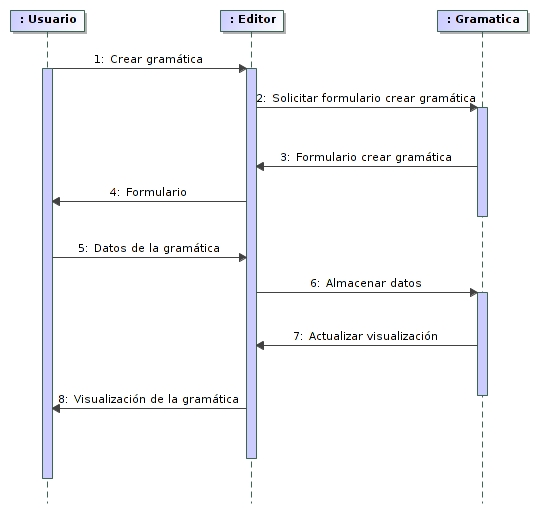
\includegraphics[scale=0.5]{img/sec3.jpg}
	\caption{Diagrama secuencia: Crear Gram�tica}
	\label{sec3}
      \end{center}
  \end{figure}
  
\section{Diagrama de secuencia: Editar vocabulario}

El diagrama de secuencia que se muestra en la figura \ref{sec4}, refleja la interacci�n de mensajes entre los objetos que participan en el caso de uso Editar Vocabulario de la gram�tica. Para ello, el usuario solicita editar el vocabulario de una gram�tica. Para llevarlo a cabo, se obtienen los s�mbolos terminales y no terminales del vocabulario para que posteriormente el usuario introduzca las modificaciones. Por �ltimo, se valida, se almacenan los datos y se actualiza la visualizaci�n para mostrar al usuario los datos introducidos.

\begin{figure}[H]
      \begin{center} 
	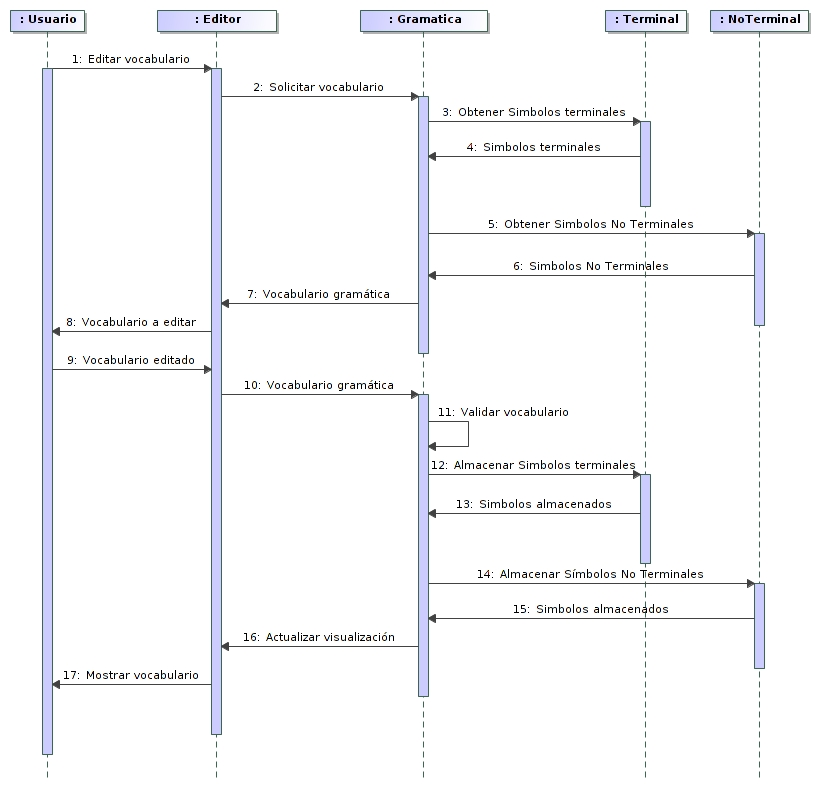
\includegraphics[scale=0.5]{img/sec4.jpg}
	\caption{Diagrama secuencia: Editar vocabulario}
	\label{sec4}
      \end{center}
  \end{figure}
  
\section{Diagrama de secuencia: Editar producci�n}

El diagrama de secuencia que se muestra en la figura \ref{sec5}, refleja la interacci�n de mensajes entre los objetos que participan en el caso de uso Editar Producci�n. Para ello, el usuario solicita editar una producci�n de la gram�tica. Para llevarlo a cabo, se obtiene el antecedente y el consecuente de la producci�n a editar para que posteriormente el usuario introduzca las modificaciones. Por �ltimo, se comprueba si la producci�n es correcta y si es as� se almacenan los datos, se actualiza la visualizaci�n para mostrar al usuario los datos introducidos.

\begin{figure}[H]
      \begin{center} 
	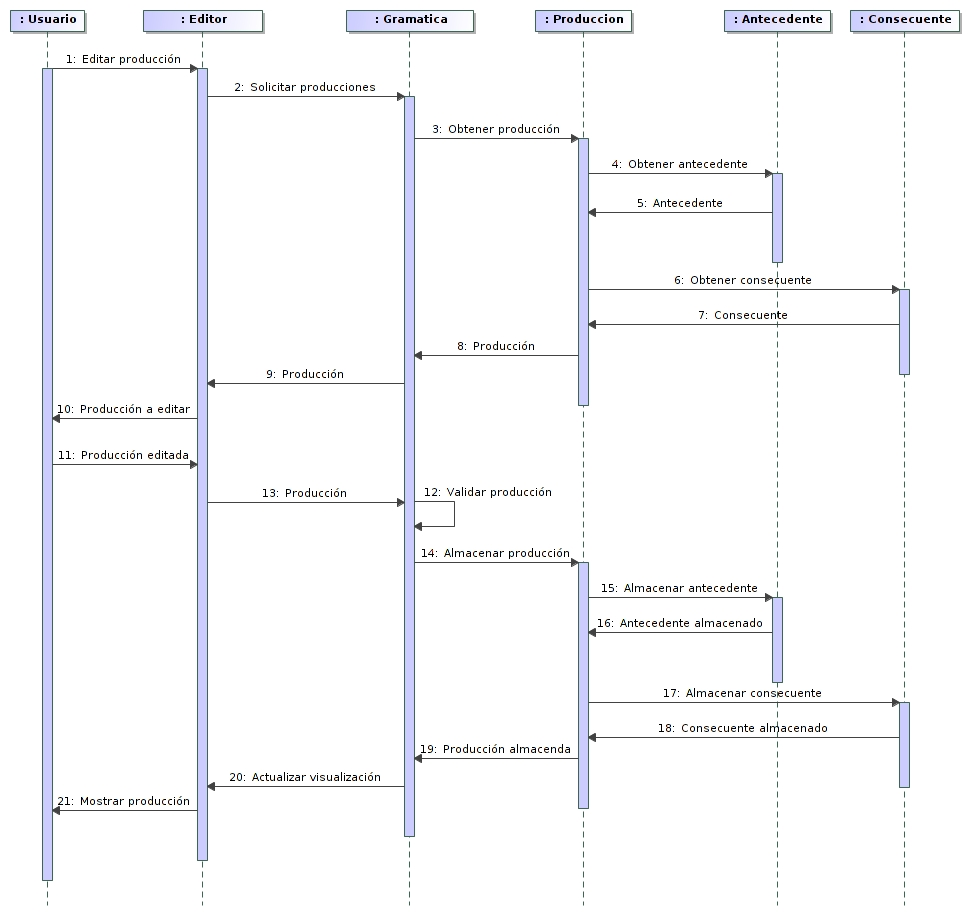
\includegraphics[angle=90, scale=0.5]{img/sec5.jpg}
	\caption{Diagrama secuencia: Editar producci�n}
	\label{sec5}
      \end{center}
  \end{figure}
  
\section{Diagrama de secuencia: Seleccionar Simbolo Inicial}

El diagrama de secuencia que se muestra en la figura \ref{sec6}, refleja la interacci�n de mensajes entre los objetos que participan en el caso de uso seleccionar Simbolo Inicial. Para ello, el usuario solicita seleccionar el s�mbolo inicial de la gram�tica. Para llevarlo a cabo, se obtiene el vocabulario de la gram�tica y se muestra al usuario los s�mbolos no terminales para que elija uno. Por �ltimo, se comprueba si la selecci�n es correcta y si es as� se almacenan los datos y se actualiza la visualizaci�n para mostrar al usuario su selecci�n.

\begin{figure}[H]
      \begin{center} 
	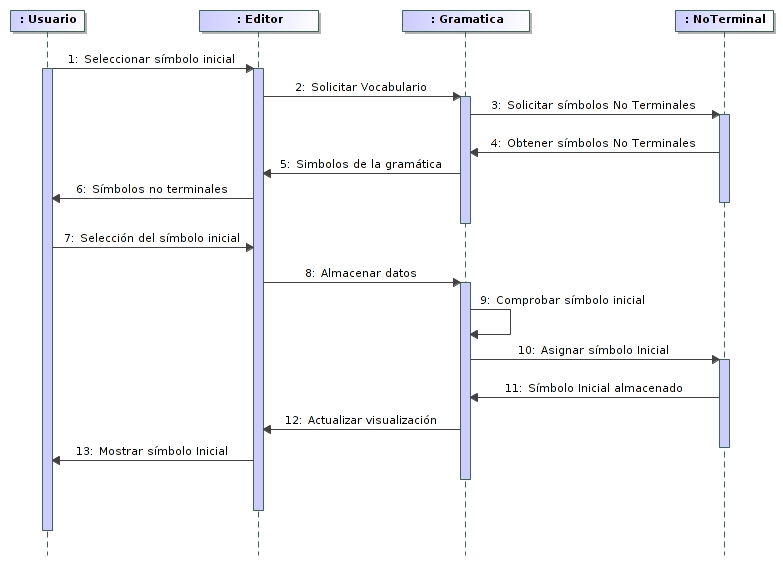
\includegraphics[scale=0.5]{img/sec6.jpg}
	\caption{Diagrama secuencia: Seleccionar S�mbolo Inicial}
	\label{sec6}
      \end{center}
  \end{figure}
  
 \newpage
\section{Diagrama de secuencia: Recuperar Gram�tica}

El diagrama de secuencia que se muestra en la figura \ref{sec7}, refleja la interacci�n de mensajes entre los objetos que participan en el caso de uso Recuperar Gram�tica. Para ello, el usuario introduce la ruta donde est� almacenada la gram�tica. Si �sta se encuentra en dicha ruta, se extrae y se actualiza la visualizaci�n.

\begin{figure}[H]
      \begin{center} 
	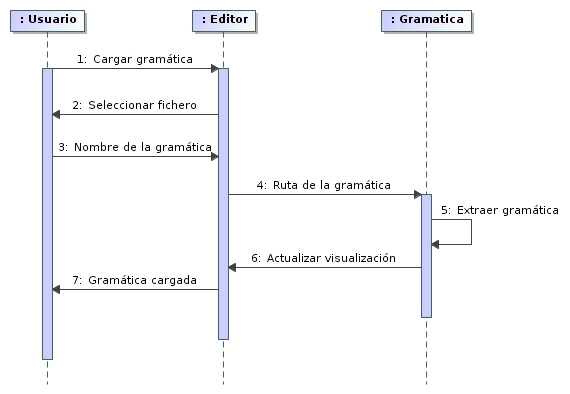
\includegraphics[scale=0.5]{img/sec7.jpg}
	\caption{Diagrama secuencia: Recuperar Gram�tica}
	\label{sec7}
      \end{center}
  \end{figure}
  
\section{Diagrama de secuencia: Validar Gram�tica}

El diagrama de secuencia que se muestra en la figura \ref{sec8}, refleja la interacci�n de mensajes entre los objetos que participan en el caso de uso Validar Gram�tica. Para ello, cuando se solicita validar la gram�tica se comprueban las producciones y si est� todo correcto se devuelve la gram�tica validada.

\begin{figure}[H]
      \begin{center} 
	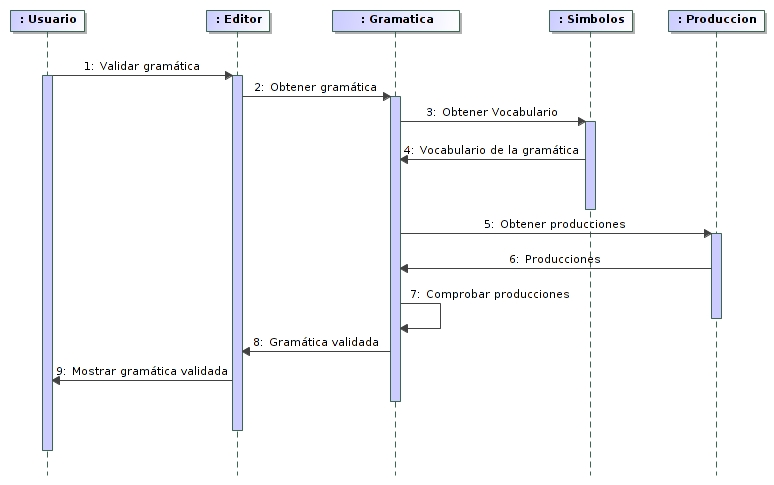
\includegraphics[scale=0.5]{img/sec8.jpg}
	\caption{Diagrama secuencia: Validar Gram�tica}
	\label{sec8}
      \end{center}
  \end{figure}
  
\section{Diagrama de secuencia: Transferir al simulador}

El diagrama de secuencia que se muestra en la figura \ref{sec9}, refleja la interacci�n de mensajes entre los objetos que participan en el caso de uso Transferir al simulador. Para ello, el usuario solicita transferir la gram�tica: si la gram�tica es v�lida entonces es enviada al simulador, que habr� sido inicializado previamente.

\begin{figure}[H]
      \begin{center} 
	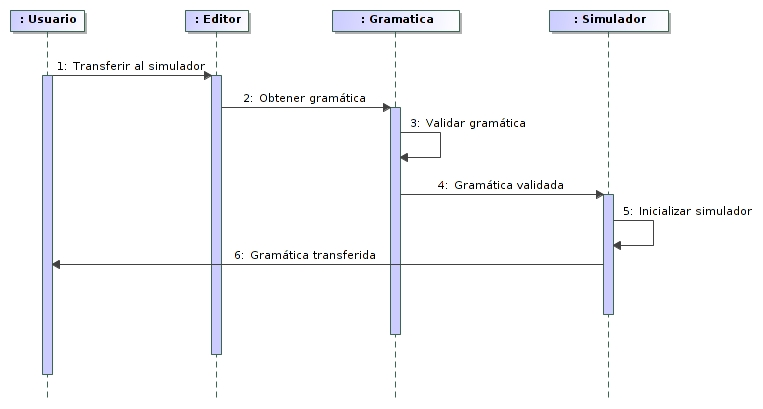
\includegraphics[scale=0.5]{img/sec9.jpg}
	\caption{Diagrama secuencia: Transferir al simulador}
	\label{sec9}
      \end{center}
  \end{figure}
  
\section{Diagrama de secuencia: Simulaci�n an�lisis Descendente}

El diagrama de secuencia que se muestra en la figura \ref{sec10}, refleja la interacci�n de mensajes entre los objetos que participan en el caso de uso Simulaci�n an�lisis Descendente. Para ello, en primer lugar se debe buscar y validar la gram�tica a simular. A continuaci�n, se debe obtener el conjunto Primero y Siguiente, la tabla predictiva y, si el usuario lo quiere, completar la tabla predictiva con funciones de error. Por �ltimo, se transfiere la gram�tica al simulador y se realiza el an�lisis de una cadena. Al final de todo el proceso el usuario obtiene el resultado de la simulaci�n.

\begin{figure}[H]
      \begin{center} 
	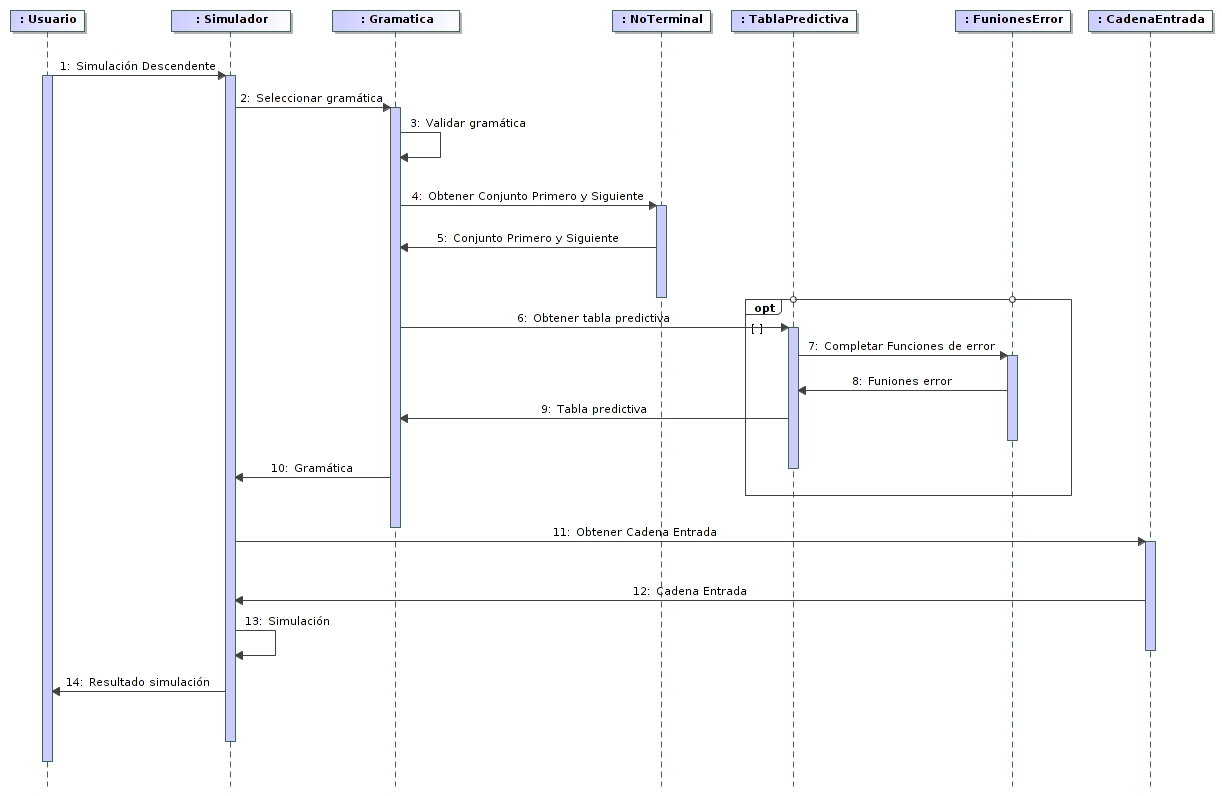
\includegraphics[angle=90, scale=0.5]{img/sec10.jpg}
	\caption{Diagrama secuencia: Simulaci�n an�lisis Descendente}
	\label{sec10}
      \end{center}
  \end{figure}
  
\section{Diagrama de secuencia: Simulaci�n an�lisis Ascendente SLR}

El diagrama de secuencia que se muestra en la figura \ref{sec11}, refleja la interacci�n de mensajes entre los objetos que participan en el caso de uso An�lisis SLR. Para ello, en primer lugar se debe buscar y validar la gram�tica a simular. A continuaci�n, se debe crear el conjunto Primero y Siguiente, la colecci�n can�nica de elementos LR(0), la tabla LR y, si el usuario lo quiere, completar la tabla LR con funciones de error. Por �ltimo, se transfiere la gram�tica al simulador y se realiza el an�lisis de una cadena. Al final de todo el proceso el usuario obtiene el resultado de la simulaci�n.
\newpage

\begin{figure}[H]
      \begin{center} 
	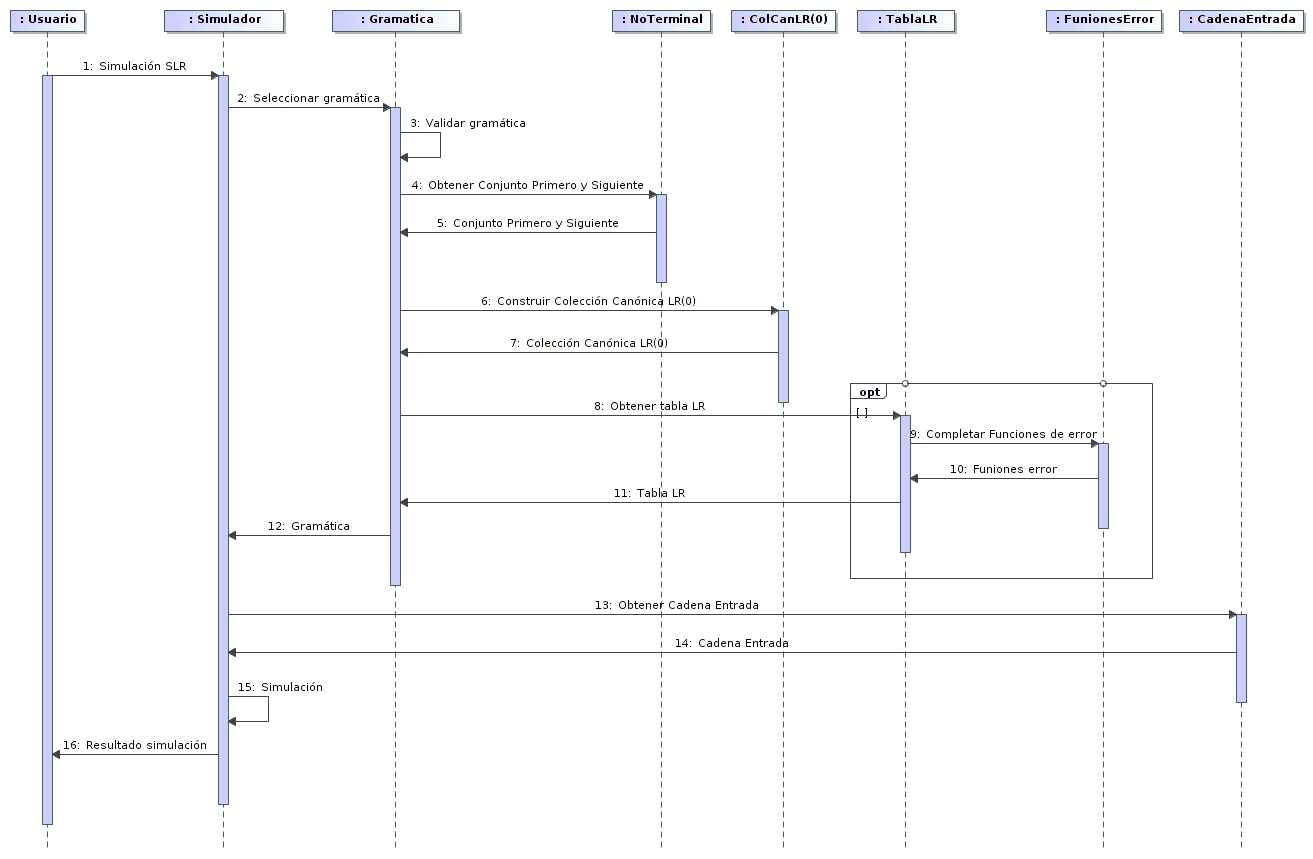
\includegraphics[angle=90, scale=0.5]{img/sec11.jpg}
	\caption{Diagrama secuencia: Simulaci�n an�lisis Ascendente SLR}
	\label{sec11}
      \end{center}
  \end{figure}
  
\section{Diagrama de secuencia: Simulaci�n an�lisis Ascendente LR-can�nico}

El diagrama de secuencia que se muestra en la figura \ref{sec12}, refleja la interacci�n de mensajes entre los objetos que participan en el caso de uso An�lisis LR-can�nico. Para ello, en primer lugar se debe buscar y validar la gram�tica a simular. A continuaci�n, se debe crear la colecci�n can�nica de elementos LR(1), la tabla LR y, si el usuario lo quiere, completar la tabla con funciones de error. Por �ltimo, se transfiere la gram�tica al simulador y se realiza el an�lisis de una cadena. Al final de todo el proceso el usuario obtiene el resultado de la simulaci�n.
\newpage

\begin{figure}[H]
      \begin{center} 
	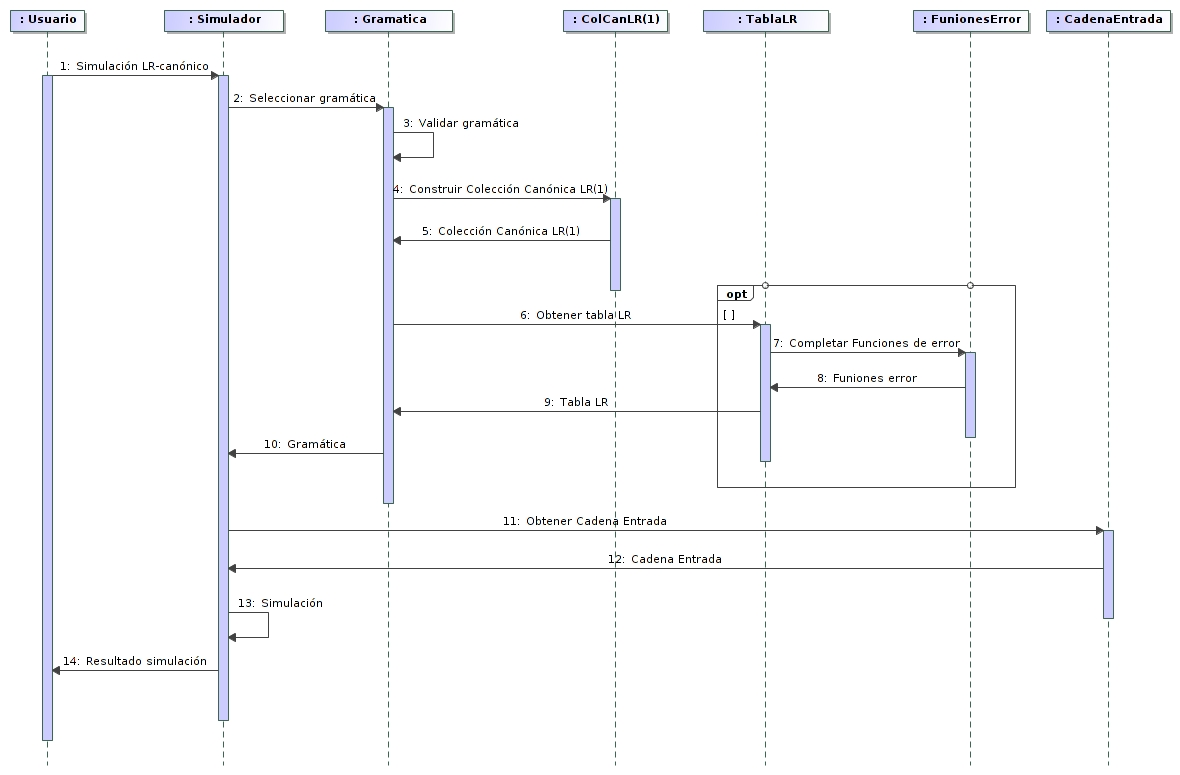
\includegraphics[angle=90, scale=0.5]{img/sec12.jpg}
	\caption{Diagrama secuencia: Simulaci�n an�lisis Ascendente LR-can�nico}
	\label{sec12}
      \end{center}
  \end{figure}
  
\section{Diagrama de secuencia: Simulaci�n an�lisis Ascendente LALR}

El diagrama de secuencia que se muestra en la figura \ref{sec13}, refleja la interacci�n de mensajes entre los objetos que participan en el caso de uso An�lisis LALR. Para ello, en primer lugar se debe buscar y validar la gram�tica a simular. A continuaci�n, se debe crear la colecci�n can�nica de elementos LALR(1), la tabla LR y, si el usuario lo quiere, completar la tabla LR con funciones de error. Por �ltimo, se transfiere la gram�tica al simulador y se realiza el an�lisis de una cadena. Al final de todo el proceso el usuario obtiene el resultado de la simulaci�n.
\newpage

\begin{figure}[H]
      \begin{center} 
	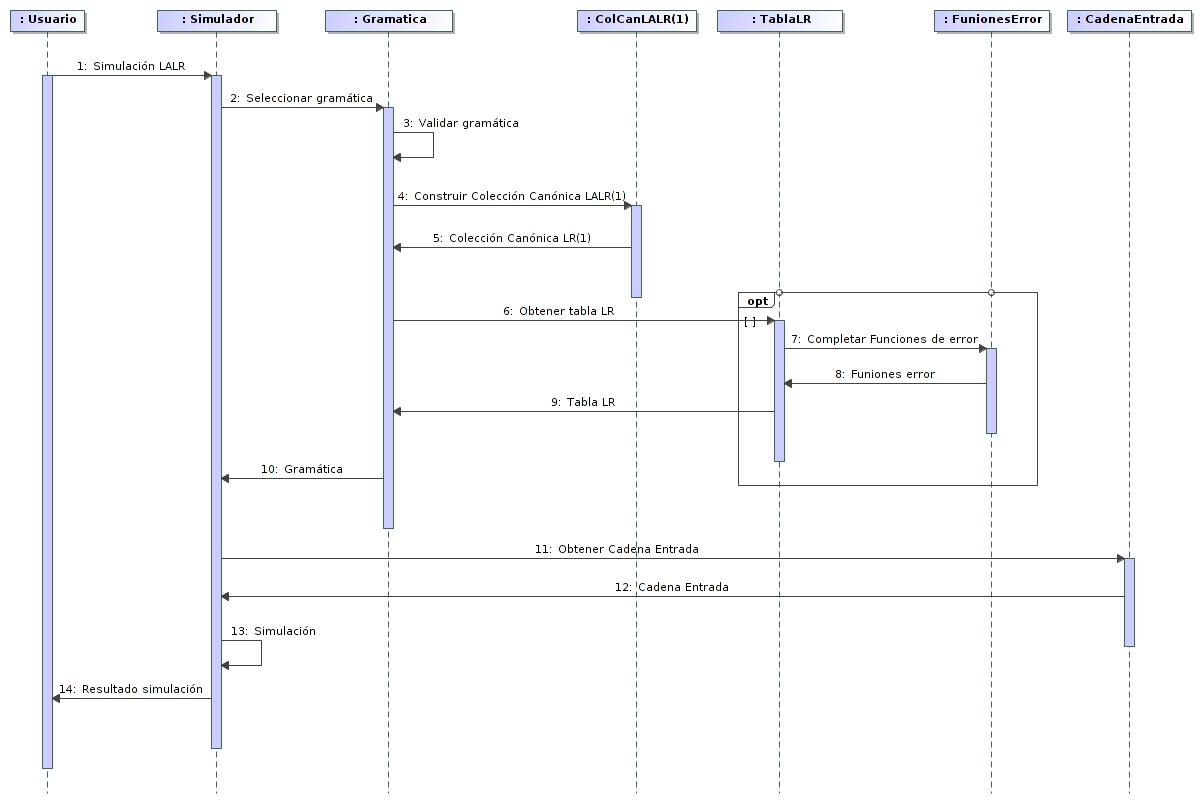
\includegraphics[angle=90, scale=0.5]{img/sec13.jpg}
	\caption{Diagrama secuencia: Simulaci�n an�lisis Ascendente LALR}
	\label{sec13}
      \end{center}
  \end{figure}

\section{Diagrama de secuencia: Tutorial}

El diagrama de secuencia que se muestra en la figura \ref{sec1}, refleja la interacci�n de mensajes entre los objetos que participan en el caso de uso Consulta del Tutorial. Para ello, el usuario solicita buscar un recurso del tutorial y una vez dentro del m�dulo el usuario podr� navegar por �l.

\begin{figure}[H]
      \begin{center} 
	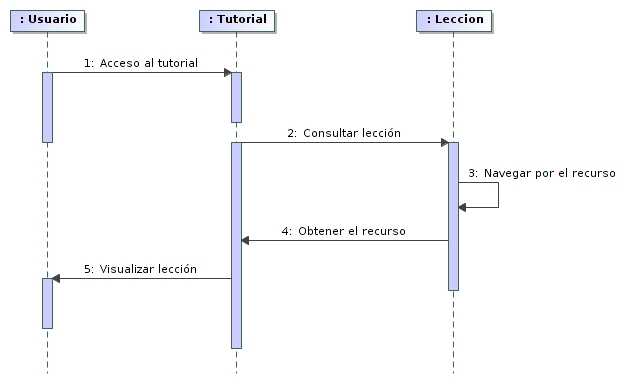
\includegraphics[scale=0.5]{img/sec1.jpg}
	\caption{Diagrama secuencia: Tutorial}
	\label{sec1}
      \end{center}
  \end{figure}

\section{Diagrama de secuencia: Ayuda}

El diagrama de secuencia que se muestra en la figura \ref{sec2}, refleja la interacci�n de mensajes entre los objetos que participan en el caso de uso Consulta de la Ayuda. Para ello, el usuario solicita buscar un recurso de la ayuda y una vez dentro del m�dulo el usuario podr� navegar por �l.

\begin{figure}[H]
      \begin{center} 
	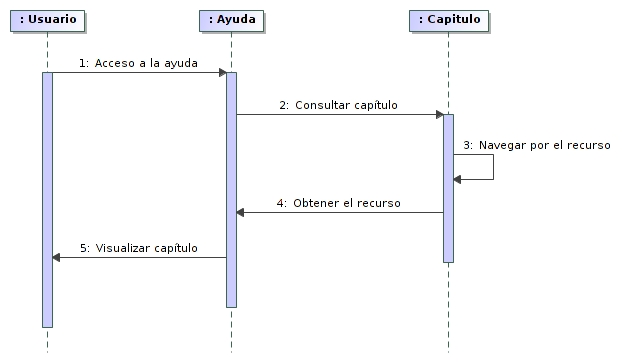
\includegraphics[scale=0.5]{img/sec2.jpg}
	\caption{Diagrama secuencia: Ayuda}
	\label{sec2}
      \end{center}
  \end{figure}













\chapter{Especificacion Requisitos de la Interfaz}

En este cap�tulo se proceder� a realizar la especificaci�n de las caracter�sticas de la \textbf{Interfaz Gr�fica de Usuario} (\textbf{IGU} en \textit{Espa�ol} o \textbf{GUI} de sus siglas en \textit{Ingl�s}).

\section{Descomposici�n de la interfaz}

La interfaz del simulador se podr�a descomponer siguiendo el mismo patr�n de descomposici�n que se utiliz� para la \textit{descomposici�n en bloques funcionales} de la aplicaci�n.

As�, siguiendo esta descomposici�n, la interfaz gr�fica de usuario tendr�a las siguientes partes o bloques:

\begin{itemize}
 \item {\textbf{SimAS}: este es el bloque principal de la interfaz. Desde �l se podr� acceder a cada uno de los 				bloques funcionales del sistema, cuya \textbf{IGU} est� representada por los siguientes bloques 						respectivamente:
      \begin{enumerate}
       \item \textbf{Editor}: esta interfaz permitir� al usuario llevar a cabo todas las acciones correspondientes a 			la edici�n de gram�ticas.
       \item \textbf{Simulador}: esta interfaz permitir� al usuario ejecutar todas las acciones del m�dulo de 						simulaci�n de gram�ticas.
       \item \textbf{Ayuda}: esta interfaz permitir� al usuario desarrollar las acciones de consulta de la ayuda.
       \item \textbf{Tutorial}: esta interfaz permitir� al usuario desarrollar las acciones de consulta del 						tutorial.
      \end{enumerate}
  }
\end{itemize}

Una vez definidos los bloques de la interfaz, cabe decir que cada bloque funcional se encuentra enlazado directamente con su correspondiente interfaz, tal y como se ha mostrado, de forma tal que la interfaz est� preparada para dar soporte a todas las acciones que se especifican en cada uno de los bloques.

En la siguiente secci�n se especificar�n cada uno de los componentes que ser�n utilizados en cada uno de los bloques de la interfaz del simulador.

\section{Especificaci�n de los componentes de la interfaz}

A continuaci�n, se analizan todos los componentes que ser�n utilizados en la interfaz, seg�n al bloque al que pertenezcan, y algunos componentes ge\-ne\-ra\-les, los cuales ser�n utilizados com�nmente por todos los dem�s bloques. 

\subsection{Componentes comunes}

Esta secci�n recoge todos los componentes comunes de la interfaz de \textbf{SimAS}. Estos componentes son los
siguientes:

\begin{enumerate}
 \item \textbf{Barra de t�tulo}.
 \item \textbf{Barra de men�s}.
 \item \textbf{Barra de herramientas}.
 \item \textbf{Men�s emergentes}.
 \item \textbf{Barra de estado}.
 \item \textbf{Di�logos}.
 \item \textbf{Texto tooltip}.
 \item \textbf{Mnem�nicos}.
 \item \textbf{Componentes b�sicos de interfaces de Swing}.
\end{enumerate}

\subsubsection{Barra de t�tulo}

La \textit{barra de t�tulo} mostrar� el nombre de la ventana de la interfaz. Este t�tulo se elegir� seg�n la funci�n que desempe�e la ventana en cuesti�n. Este componente se situar� en la parte superior de cada una de las ventanas del simulador.

\subsubsection{Barra de men�s}

La \textit{barra de men�} ser� usada en las ventanas para mostrar acciones de men� (que variar�n seg�n la funcionalidad de cada ventana). La barra de men�s se situar� justamente debajo de la barra de t�tulo de la ventana.

\subsubsection{Barra de herramientas}

Contendr� botones que representar�n de forma visual las acciones que el usuario puede llevar a cabo en una ventana determinada. En definitiva, se trata de accesos directos a las acciones m�s comunes de una ventana (para evitar tener que navegar tediosamente por los men�s de la aplicaci�n y facilitar la navegabilidad de la interfaz). La barra de herramientas se sit�a justo debajo de la barra de men�s de la ventana.

Cada uno de los botones de la barra de herramientas tendr� asociado una imagen, que ser� lo m�s descriptiva posible (de cara a hacer m�s f�cil la labor del usuario a la hora de utilizar la aplicaci�n).

\subsubsection{Men�s emergentes}

Estos men�s mostrar�n al usuario ciertas acciones asociadas a elementos de la interfaz. El men� podr� o no estar presente en las ventanas del simulador y siempre estar� asociado a un componente de la interfaz (bot�n, lista, etc�tera) concreto. El men� se mostrar� al hacer clic con el bot�n derecho del rat�n sobre el componente.

\subsubsection{Barra de estado}

Esta barra mostrar� informaci�n sobre el estado actual de la ventana y se mostrar� en la parte inferior de la ventana.

\subsubsection{Di�logos}

Se trata de peque�as ventanas con barra de t�tulo propia que se muestran para indicar al usuario la ocurrencia de un evento determinado (mostrar un mensaje, informar de un error, etc�tera).

\subsubsection{Texto tooltip}

Cada componente de la interfaz tendr� asociado un texto peque�o que describir� el componente (o explicar� su uso o acci�n) y que ser� mostrado cuando el usuario sit�e el rat�n justo encima del componente, sin necesidad de pulsar ning�n bot�n del rat�n.

\subsubsection{Mnem�nicos}

Algunos componentes o acciones de la interfaz podr�n tener asociados accesos directos, para mejorar el uso de la aplicaci�n.

Estos \textit{mnem�nicos} ser�n mostrados tambi�n en las correspondientes opciones del men� de la ventana, donde se especificar� la combinaci�n de teclas asociada como acceso directo a ese componente (ejemplo: \textbf{F1} para acceder a la ayuda de la aplicaci�n).

Adem�s, los men�s podr�n ser utilizados pulsando la tecla \textbf{ALT} y una letra, la cual ser� resaltada mediante un subrayado en la interfaz de usuario. Esta funcionalidad se a�adir� tanto a los men�s como a todos los submen�s de las ventanas de \textbf{SimAS}.

\subsubsection{Componentes b�sicos de interfaces de Swing}

Las ventanas del simulador utilizar�n tambi�n los componentes b�sicos que proporciona \textit{Swing}, tales como botones, cuadros de texto, listas, cuadros de selecci�n, etiquetas, canvas de dibujo, etc�tera.

\subsection{Componentes espec�ficos de la interfaz}

En esta secci�n se detallar�n los componentes espec�ficos que se integrar�n en cada uno de los m�dulos de la interfaz para as� poder desarrollar su cometido.

\subsubsection{M�dulo de edici�n de gram�ticas}

En este m�dulo, se emplear�n componentes Swing para la visualizaci�n de \textit{c�digo HTML}, para as� representar gram�ticas de contexto libre. Adem�s, se utilizar�n m�dulos para la generaci�n de documentos pdf (para generar informes).

\subsubsection{M�dulo de simulaci�n}

En este m�dulo se emplear�n componentes para la visualizaci�n de gram�ticas y la generaci�n de documentos pdf, al igual que en el m�dulo anterior.

Adem�s, se emplear� un m�dulo para la representaci�n visual de la tabla predictiva y de la tabla LR y las funciones de error (y la tabla de an�lisis durante la simulaci�n).

\subsubsection{M�dulo de la ayuda}

Para la ayuda, se emplear� un componente para visualizar los cap�tulos que la componen y un \textit{visualizador HTML} para visualizarlos.

\subsubsection{M�dulo del tutorial}

Los componentes que ser�n empleados en la interfaz del tutorial son id�nticos a los que se emplean en la ayuda.





\part{Dise�o}



\chapter{Dise�o de clases}

En este cap�tulo se realizar� una breve introducci�n sobre el diagrama de clases y posteriormente, un an�lisis de las clases que participan en el modelo de informaci�n del simulador. Para ello, se especificar�n los atributos, m�todos y las relaciones existentes entre las mismas, termin�ndose con un diagrama de clases general de todo el sistema.

\section{Introducci�n}

El prop�sito de un diagrama de clases es el de representar los objetos fundamentales del sistema, es decir, los que percibe el usuario y con los que espera tratar para completar su tarea. Una clase define el �mbito de definici�n de un conjunto de objetos.

Cada clase se representa en un rect�ngulo con tres apartados:
\begin{itemize}
\item Nombre de la clase.

\item Atributos de la clase.

\item Operaciones de la clase.
\end{itemize}


\section{Clases del sistema}

Seg�n el an�lisis del sistema realizado hasta ahora,las clases \textbf{principales} que componen el sistema son las siguientes:

\begin{itemize}
 \item SimAS.
 \item Editor.
 \item Simulador.
 \item Ayuda.
 \item Tutorial.
 
\end{itemize}

Las clases que ser�n utilizadas por la clase \textbf{Editor} son las siguientes:

\begin{itemize}
 \item Gramatica.
 \item Produccion.
 \item Consecuente.
 \item Antecedente.
 \item NoTerminal.
 \item Terminal.
 \item Simbolo.
 \item TablaPredictiva.
 \item TablaLR.
 \item ParteIrA.
 \item ParteAccion.
 \item FuncionesError.
 \item ColCanLR(0).
 \item ColCanLR(1).
 \item ColCanLALR(1).
 \item ConjElementosLR(0).
 \item ConjElementosLR(1).
 \item ConjElementosLALR(1).
 \item ElementosLR(0).
 \item ElementosLR(1).
 \item ElementosLALR(1).

\end{itemize}

Las clases que ser�n utilizadas por la clase \textbf{Simulador} son las siguientes:
 
 \begin{itemize}
 \item Gram�tica.
 \item CadenaEntrada.
 \end{itemize}
 
 Las clases que se encuentran contenidas dentro de la clase \textbf{Ayuda} son las siguientes:
 
 \begin{itemize}
  \item Cap�tulo.
 \end{itemize}
 
 Las clases que se encuentran contenidas dentro de la clase \textbf{Tutorial} son las siguientes:

\begin{itemize}
 \item Lecci�n.
\end{itemize}


A continuaci�n se har� un an�lisis de cada una de las clases que se han definido anteriormente.

\subsection{Clase SimAS}

Esta clase representa a la clase principal del Sistema y es la que se encarga de inicializar los dem�s componentes de la aplicaci�n. En la tabla \ref{tabla81} se recoge la especificaci�n de la clase
y en la figura \ref{clase1} se muestra su representaci�n gr�fica.

\begin{longtable}[H]{|>{\columncolor[rgb]{0.63,0.79,0.95}}m{6cm} | m{8.5cm} |}
 \caption{Clase SimAS}

\endfirsthead

\multicolumn{2}{c}
{{\tablename\ \thetable{} -- contin�a de la p�gina anterior}} \\
\endhead

\hline \multicolumn{2}{|r|}{{Contin�a en la p�gina siguiente}} \\ \hline
\endfoot

\hline
\endlastfoot

\hline
 \textbf{Nombre} & \textbf{SimAS}  \\ \hline
 
 \textbf{Descripci�n} & Representa la clase principal del simulador.  \\ \hline
                       
 \textbf{Atributos} & No posee ning�n atributo. \\ \hline
 
 \textbf{M�todos} & \begin{enumerate}
                	\item \textbf{init}: m�todo p�blico que permite \textit{inicializar} los componentes 										de la aplicaci�n.
                	\item \textbf{lanzarEditor}: m�todo p�blico que permite \textit{lanzar} el m�dulo Editor del 								simulador.
                	\item \textbf{lanzarSimulador}: m�todo p�blico que permite \textit{lanzar} el m�dulo Simulador del 						simulador.
                	\item \textbf{lanzarAyuda}: m�todo p�blico que permite \textit{lanzar} el m�dulo Ayuda del 								simulador.
                	\item \textbf{lanzarTutorial}: m�todo p�blico que permite \textit{lanzar} el m�dulo Tutorial del 							simulador.
             \end{enumerate} 
                                 
 \label{tabla81}

\end{longtable}

 \begin{figure}[H]
      \begin{center} 
	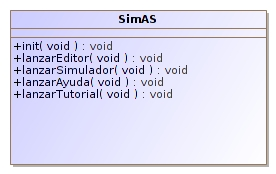
\includegraphics[scale=0.5]{img/clase1.jpg}
	\caption{Representaci�n gr�fica de la clase SimAS}
	\label{clase1}
      \end{center}
  \end{figure}
  
\subsection{Clase Editor}

Esta clase representa al editor de gram�ticas y es la que se encarga de editar las gram�ticas de contexto
libre. En la tabla \ref{tabla82} se recoge la especificaci�n de la clase y en la figura \ref{clase2} se muestra su representaci�n gr�fica.
  
  
  \begin{longtable}[H]{|>{\columncolor[rgb]{0.63,0.79,0.95}}m{6cm} | m{8.5cm} |}
 \caption{Clase Editor}

\endfirsthead

\multicolumn{2}{c}
{{\tablename\ \thetable{} -- contin�a de la p�gina anterior}} \\
\endhead

\hline \multicolumn{2}{|r|}{{Contin�a en la p�gina siguiente}} \\ \hline
\endfoot

\hline
\endlastfoot

\hline
 \textbf{Nombre} & \textbf{Editor}  \\ \hline
 
 \textbf{Descripci�n} & Representa a un editor de gram�ticas.  \\ \hline
                       
 \textbf{Atributos} & \begin{enumerate}
 		\item \textbf{gramatica}: instancia de una \textit{gram�tica} que podr� ser utilizada por el editor. 
       \end{enumerate}  \\ \hline
 
 \textbf{M�todos} & \begin{enumerate}
		\item \textbf{cargarGramatica}: m�todo p�blico que permite cargar una gram�tica desde un archivo.
		\item \textbf{grabarGramatica}: m�todo p�blico que permite grabar una gram�tica en un fichero.
		\item \textbf{crearGramatica}: m�todo p�blico que permite la creaci�n de una nueva gram�tica.
		\item \textbf{getGramatica}: m�todo p�blico que permite obtener una gram�tica.
		\item \textbf{setGramatica}: m�todo p�blico que permite editar una gram�tica.
		\item \textbf{actualizarVisualizacion}: m�todo privado que permite actualizar la	visualizaci�n de la 						gram�tica en el editor.
        \end{enumerate}
                                 
 \label{tabla82}

\end{longtable}

 \begin{figure}[H]
      \begin{center} 
	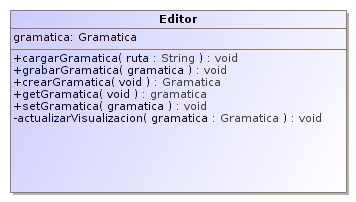
\includegraphics[scale=0.5]{img/clase2.jpg}
	\caption{Representaci�n gr�fica de la clase Editor}
	\label{clase2}
      \end{center}
  \end{figure}

\subsection{Clase Gramatica}

Esta clase representa a las gram�ticas de contexto libre. En la tabla \ref{tabla83}
se recoge la especificaci�n de la clase y en la figura \ref{clase3} se muestra
su representaci�n gr�fica.

\begin{longtable}[H]{|>{\columncolor[rgb]{0.63,0.79,0.95}}m{6cm} | m{8.5cm} |}
 \caption{Clase Gramatica}

\endfirsthead

\multicolumn{2}{c}
{{\tablename\ \thetable{} -- contin�a de la p�gina anterior}} \\
\endhead

\hline \multicolumn{2}{|r|}{{Contin�a en la p�gina siguiente}} \\ \hline
\endfoot

\hline
\endlastfoot

\hline
 \textbf{Nombre} & \textbf{Gramatica}  \\ \hline
 
 \textbf{Descripci�n} & Representa a las gram�ticas de contexto libre.  \\ \hline
                       
 \textbf{Atributos} & \begin{enumerate}
 		\item \textbf{nombre}: este atributo representa el nombre de la gram�tica de contexto libre.
 		\item \textbf{terminales}: este atributo representa el conjunto de s�mbolos terminales.
 		\item \textbf{noTerminales}: este atributo representa el conjunto de s�mbolos no terminales.
		 \item \textbf{producciones}: este atrobito representa el conjunto de producciones de la gram�tica.
		 \item \textbf{descripcion}: este atributo representa la descripci�n de la gram�tica.
 		 \item \textbf{TPredictiva}: este atributo representa la tabla predictiva de la gram�tica.
\end{enumerate}\\ \hline
	
 \textbf{Atributos} & \begin{enumerate}
		\setcounter{enumi}{6}

		 \item \textbf{TLR}: este atributo representa la tabla LR de la gram�tica.
		 \item \textbf{coleccionLR0}: este atributo representa la colecci�n can�nica de elementos LR(0).
		 \item \textbf{coleccionLR1}: este atributo representa la colecci�n can�nica de elementos LR(1).
 		 \item \textbf{coleccionLALR1}: este atributo representa la colecci�n can�nica de elementos LALR(1).
		\end{enumerate} \\ \hline
 
 \textbf{M�todos} & \begin{enumerate}
 		\item \textbf{getNombre}: m�todo p�blico que permite obtener el nombre de la gram�tica de contexto libre.
 		\item \textbf{setNombre}: m�todo p�blico que permite editar el nombre de la gram�tica de contexto libre.
 		\item \textbf{getVocabulario}: m�todo p�blico que permite obtener el vocabulario (s�mbolos terminales y no 				terminales) de una gram�tica.
		\item \textbf{setVocabulario}: m�todo p�blico que permite editar el vocabulario (s�mbolos terminales y no 				terminales) de una gram�tica.
		\item \textbf{crearSimbolo}: m�todo p�blico que permite crear un s�mbolo de la gram�tica, terminal o no 					terminal.
		
			\end{enumerate}\\ \hline
	
	 \textbf{M�todos} & \begin{enumerate}
		\setcounter{enumi}{5}
		\item \textbf{eliminarSimbolo}: m�todo p�blico que permite eliminar un s�mbolo de la gram�tica, terminal o 				no terminal. Al eliminar un s�mbolo autom�ticamente se eliminar�n las producciones en las que aparezca 				�ste.
		\item \textbf{crearProduccion}: m�todo p�blico que permite a�adir el antecedente y el consecuente de una 					producci�n.
		\item \textbf{getProduccion}: m�todo p�blico que permite obtener la producci�n, esto es, el antecedente y el 			consecuente.
				
		\item \textbf{setProduccion}: m�todo p�blico que permite editar el antecedente, el consecuente o ambos de 			un producci�n.
		\item \textbf{eliminarProducci�n}: m�todo p�blico que permite eliminar una producci�n, esto es, tanto el 					antecedente como el consecuente.
		\item \textbf{getDescripcion}: m�todo p�blico que permite obtener la descrici�n de la gram�tica.
		\item \textbf{setDescripcion}: m�todo p�blico que permite editar la descrici�n de la gram�tica.
		\item \textbf{generarInforme}: m�todo p�blico que permite generar un informe PDF de la gram�tica.
		\item \textbf{selecSimboloInicial}: m�todo p�blico que permite seleccionar el s�mbolo inicial de la 						gram�tica.
		
		\end{enumerate}\\ \hline
	
	 \textbf{M�todos} & \begin{enumerate}
		\setcounter{enumi}{14}
		\item \textbf{getSimboloInicial}: m�todo p�blico que permite obtener el s�mbolo inicial de la gram�tica.
		\item \textbf{transferirGramatica}: m�todo p�blico que permite transferir la	gram�tica al simulador.
		\item \textbf{validarGramatica}: m�todo p�blico que permite validar la gram�tica.
			
		\item \textbf{generarConjPrim}: m�todo p�blico que permite generar el conjunto Primero de la 								gram�tica.
		\item \textbf{getConjPrim}: m�todo p�blico que permite obtener el conjunto primero de la gram�tica.
		\item \textbf{generarConjSig}: m�todo p�blico que permite generar el conjunto Siguiente de la 							gram�tica.
		\item \textbf{getConjSig}: m�todo p�blico que permite obtener el conjunto siguiente de la gram�tica.
		\item \textbf{generarTPredictiva}: m�todo p�blico que permite generar la tabla predictiva para realizar el 				an�lisis sint�ctico descendente.
		\item \textbf{getTPredictiva}: m�todo p�blico que permite obtener la tabla predictiva de la gram�tica.
		\item \textbf{generarTLR}: m�todo p�blico que permite generar la tabla LR para realizar el an�lisis 						sint�ctico ascendente.
		\item \textbf{getTLR}: m�todo p�blico que permite obtener la tabla LR de la gram�tica.
		
		\end{enumerate}\\ \hline
	
	 \textbf{M�todos} & \begin{enumerate}
		\setcounter{enumi}{25}
		\item \textbf{generarColCanLR0}: m�todo p�blico que permite generar la colecci�n can�nica de elementos 					LR(0).
		\item \textbf{getColCanLR0}: m�todo m�todo p�blico que permite obtener la colecci�n can�nica LR(0) de la 					gram�tica.
		\item \textbf{generarColCanLR1}: m�todo p�blico que permite generar la colecci�n can�nica de elementos 					LR(1).
		\item \textbf{getColCanLR1}: m�todo p�blico que permite obtener la colecci�n can�nica LR(1) de la gram�tica.
		\item \textbf{generarColCanLALR1}: m�todo p�blico que permite generar la colecci�n can�nica de elementos 					LALR(1).
		\item \textbf{getColCanLALR1}: m�todo p�blico que permite obtener la colecci�n can�nica LALR(1) de la 					gram�tica.
      \end{enumerate}
                                 
 \label{tabla83}

\end{longtable}


\begin{figure}[H]
      \begin{center} 
	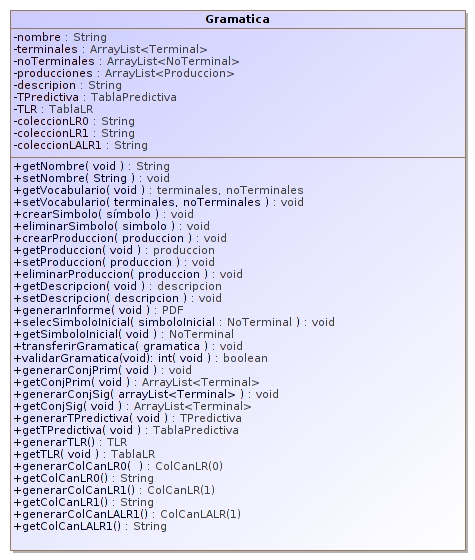
\includegraphics[scale=0.5]{img/clase3.jpg}
	\caption{Representaci�n gr�fica de la clase Gramatica}
	\label{clase3}
      \end{center}
  \end{figure}

\subsection{Clase Simbolo}

Esta clase representa a cualquier s�mbolo de la gram�tica (terminal o no terminal). En la tabla \ref{tabla84} se recoge la especificaci�n de la clase y en la figura \ref{clase4} se muestra
su representaci�n gr�fica.
\newpage

\begin{longtable}[H]{|>{\columncolor[rgb]{0.63,0.79,0.95}}m{6cm} | m{8.5cm} |}
 \caption{Clase Simbolo}

\endfirsthead

\multicolumn{2}{c}
{{\tablename\ \thetable{} -- contin�a de la p�gina anterior}} \\
\endhead

\hline \multicolumn{2}{|r|}{{Contin�a en la p�gina siguiente}} \\ \hline
\endfoot

\hline
\endlastfoot

\hline
 \textbf{Nombre} & \textbf{Simbolo}  \\ \hline
 
 \textbf{Descripci�n} & Representa a cualquier s�mbolo de la gram�tica.  \\ \hline
                       
 \textbf{Atributos} & \begin{enumerate}
 		\item \textbf{nombre}: \textit{nombre} del s�mbolo. Si no es un car�cter especial, contendr� la 					representaci�n del s�mbolo.
 		\item \textbf{valor}: este atributo almacena la \textit{representaci�n} del s�mbolo (el c�digo 					unicode en caso de que el s�mbolo fuera especial, como $ \epsilon $).
	\end{enumerate} \\ \hline
 
 \textbf{M�todos}& \begin{enumerate}
 		\item \textbf{getNombre}: m�todo p�blico que permite obtener el nombre del s�mbolo. 
		 \item \textbf{getValor}: m�todo p�blico que permite obtener el valor del s�mbolo. 
 		\item \textbf{setNombre}: m�todo p�blico que permite asignar el nombre del s�mbolo. 
 		\item \textbf{setValor}: m�todo p�blico que permite asignar el valor del 	s�mbolo. 
 		
		\end{enumerate}
                                 
 \label{tabla84}

\end{longtable}

 \begin{figure}[H]
      \begin{center} 
	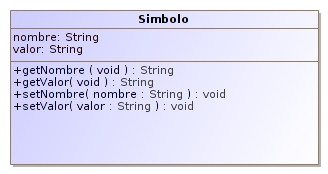
\includegraphics[scale=0.5]{img/clase4.jpg}
	\caption{Representaci�n gr�fica de la clase Simbolo}
	\label{clase4}
      \end{center}
  \end{figure}
  
\subsection{Clase Terminal}

Esta clase representa a cualquier s�mbolo terminal de la gram�tica, la cual hereda todos los atributos y m�todos de la clase S�mbolo. En la tabla \ref{tabla85}
se recoge la especificaci�n de la clase y en la figura \ref{clase5} se muestra
su representaci�n gr�fica.

\begin{longtable}[H]{|>{\columncolor[rgb]{0.63,0.79,0.95}}m{6cm} | m{8.5cm} |}
 \caption{Clase Terminal}

\endfirsthead

\multicolumn{2}{c}
{{\tablename\ \thetable{} -- contin�a de la p�gina anterior}} \\
\endhead

\hline \multicolumn{2}{|r|}{{Contin�a en la p�gina siguiente}} \\ \hline
\endfoot

\hline
\endlastfoot

\hline
 \textbf{Nombre} & \textbf{Terminal}  \\ \hline
 
 \textbf{Descripci�n} & Representa a los s�mbolos terminales de la gram�tica.  \\ \hline
                       
 \textbf{Atributos} & Hereda los atributos de la clase S�mbolo. \\ \hline
 
 \textbf{M�todos} & Hereda los m�todos de la clase S�mbolo.
                                 
 \label{tabla85}

\end{longtable}

 \begin{figure}[H]
      \begin{center} 
	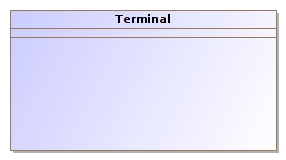
\includegraphics[scale=0.5]{img/clase5.jpg}
	\caption{Representaci�n gr�fica de la clase Terminal}
	\label{clase5}
      \end{center}
  \end{figure}


\subsection{Clase NoTerminal}

Esta clase representa a cualquier s�mbolo no terminal de la gram�tica, la cual hereda todos los atributos y m�todos de la clase S�mbolo. En la tabla \ref{tabla86} se recoge la especificaci�n de la clase y en la figura \ref{clase6} se muestra su representaci�n gr�fica.

\newpage

\begin{longtable}[H]{|>{\columncolor[rgb]{0.63,0.79,0.95}}m{6cm} | m{8.5cm} |}
 \caption{Clase NoTerminal}

\endfirsthead

\multicolumn{2}{c}
{{\tablename\ \thetable{} -- contin�a de la p�gina anterior}} \\
\endhead

\hline \multicolumn{2}{|r|}{{Contin�a en la p�gina siguiente}} \\ \hline
\endfoot

\hline
\endlastfoot

\hline
 \textbf{Nombre} & \textbf{NoTerminal}  \\ \hline
 
 \textbf{Descripci�n} & Representa a los s�mbolos no terminales de la gram�tica.  \\ \hline
                       
 \textbf{Atributos} & \begin{enumerate}
 		 \item \textbf{simboloInicial}: indica si el s�mbolo no terminal es inicial o no.
 		 \item \textbf{primeros}: lista de s�mbolos terminales que forman el conjunto primero del s�mbolo terminal, 				tambi�n 	puede contener $\epsilon$.
 		 \item \textbf{siguientes}: lista de s�mbolos terminales que forman el conjunto siguiente del s�mbolo 					no terminal, tambi�n puede contener \$.
		\end{enumerate}  \\ \hline
 
 \textbf{M�todos} & \begin{enumerate}
 		\item \textbf{getSimInicial}: m�todo p�blico que \textit{devuelve} si el s�mbolo es inicial o no.
 		\item \textbf{setSimInicial}: m�todo p�blico que \textit{permite asignar} el valor 1 si el s�mbolo terminal 				es el s�mbolo	inicial y el valor 0 en el caso contrario.
 		\item \textbf{getPrimeros}: m�todo p�blico que \textit{devuelve} el conjunto Primero del s�mbolo no 						terminal.
 		\item \textbf{setPrimeros}: m�todo p�blico que permite almacenar la lista de s�mbolos terminales 							que forman parte del conjunto Primero.
 		\item \textbf{getSiguientes}: m�todo p�blico que devuelve el conjunto Siguiente del s�mbolo no 							terminal.
 			\end{enumerate}\\ \hline
	
 \textbf{M�todos} & \begin{enumerate}
		\setcounter{enumi}{5}
 		
 		\item \textbf{setSiguientes}: m�todo p�blico que permite almacenar la lista de s�mbolos terminales 						que 	forman parte del conjunto Siguiente.
 
 		\end{enumerate}
                                 
 \label{tabla86}

\end{longtable}

 \begin{figure}[H]
      \begin{center} 
	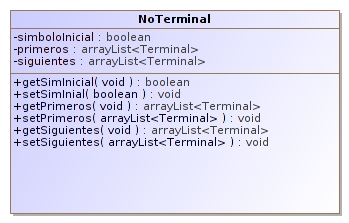
\includegraphics[scale=0.5]{img/clase6.jpg}
	\caption{Representaci�n gr�fica de la clase NoTerminal}
	\label{clase6}
      \end{center}
  \end{figure}


\subsection{Clase Produccion}

Esta clase representa a las producciones de la gram�tica. En la tabla \ref{tabla88} se recoge la especificaci�n de la clase y en la figura \ref{clase8} se muestra su representaci�n gr�fica.

\begin{longtable}[H]{|>{\columncolor[rgb]{0.63,0.79,0.95}}m{6cm} | m{8.5cm} |}
 \caption{Clase Produccion}

\endfirsthead

\multicolumn{2}{c}
{{\tablename\ \thetable{} -- contin�a de la p�gina anterior}} \\
\endhead

\hline \multicolumn{2}{|r|}{{Contin�a en la p�gina siguiente}} \\ \hline
\endfoot

\hline
\endlastfoot

\hline
 \textbf{Nombre} & \textbf{Produccion}  \\ \hline
 
 \textbf{Descripci�n} & Representa a los producciones de la gram�tica.  \\ \hline
                       
 \textbf{Atributos} & \begin{enumerate}
 		\item \textbf{antec}: representa al \textit{antecedente} de la producci�n (s�mbolo no 								terminal).
 		\item \textbf{consec}: representa al \textit{consecuente} de la producci�n (que es una lista de 						s�mbolos terminales y no terminales, o lo que es lo mismo, de s�mbolos gramaticales). Tambi�n puede ser 				el s�mbolo $\epsilon$.
		\end{enumerate}\\ \hline
 
 \textbf{M�todos} & \begin{enumerate}
 		\item \textbf{getAntecedente}: m�todo p�blico que devuelve el antecedente de una producci�n.
 		\item \textbf{setAntecedente}: m�todo p�blico que permite almacenar el antecedente de una producci�n.
 		\item \textbf{getConsecuente}: m�todo p�blico que devuelve el consecuente de una producci�n.
 		\item \textbf{setConsecuente}: m�todo p�blico que permite almacenar el consecuente de una producci�n. 

\end{enumerate}
                                 
 \label{tabla88}

\end{longtable}

 \begin{figure}[H]
      \begin{center} 
	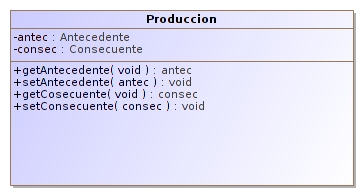
\includegraphics[scale=0.5]{img/clase8.jpg}
	\caption{Representaci�n gr�fica de la clase Produccion}
	\label{clase8}
      \end{center}
  \end{figure}

\subsection{Clase Antecedente}

Esta clase representa al antecedente de la producci�n de una gram�tica. En la tabla \ref{tabla89} se recoge la especificaci�n de la clase y en la figura \ref{clase9} se muestra su representaci�n gr�fica.

\begin{longtable}[H]{|>{\columncolor[rgb]{0.63,0.79,0.95}}m{6cm} | m{8.5cm} |}
 \caption{Clase Antecedente}

\endfirsthead

\multicolumn{2}{c}
{{\tablename\ \thetable{} -- contin�a de la p�gina anterior}} \\
\endhead

\hline \multicolumn{2}{|r|}{{Contin�a en la p�gina siguiente}} \\ \hline
\endfoot

\hline
\endlastfoot

\hline
 \textbf{Nombre} & \textbf{Antecedente}  \\ \hline
 
 \textbf{Descripci�n} & Representa al antecedente de una producci�n.  \\ \hline
                       
 \textbf{Atributos} & \begin{enumerate}
 		\item \textbf{simboloNT}: representa el s�mbolo no terminal que forma parte del antecedente de una 						producci�n.
 		\end{enumerate} \\ \hline
 
 \textbf{M�todos} & \begin{enumerate}
  		\item \textbf{getSimboloNT}: m�todo p�blico que permite obtener el s�mbolo no terminal que forma parte del 				antecedente de la producci�n.
  		\item \textbf{setSimboloNT}: m�todo p�blico que permite asignar un s�mbolo no terminal de la gram�tica 					definida al	antecedente de la producci�n.
  \end{enumerate}
                                
 \label{tabla89}

\end{longtable}

 \begin{figure}[H]
      \begin{center} 
	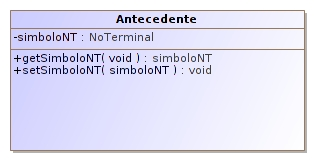
\includegraphics[scale=0.5]{img/clase9.jpg}
	\caption{Representaci�n gr�fica de la clase Antecedente}
	\label{clase9}
      \end{center}
  \end{figure}

\subsection{Clase Consecuente}

Esta clase representa al consecuente de la producci�n de una gram�tica. En la tabla \ref{tabla810} se recoge la especificaci�n de la clase y en la figura \ref{clase10} se muestra su representaci�n gr�fica.

\begin{longtable}[H]{|>{\columncolor[rgb]{0.63,0.79,0.95}}m{6cm} | m{8.5cm} |}
 \caption{Clase Consecuente}

\endfirsthead

\multicolumn{2}{c}
{{\tablename\ \thetable{} -- contin�a de la p�gina anterior}} \\
\endhead

\hline \multicolumn{2}{|r|}{{Contin�a en la p�gina siguiente}} \\ \hline
\endfoot

\hline
\endlastfoot

\hline
 \textbf{Nombre} & \textbf{Consecuente}  \\ \hline
 
 \textbf{Descripci�n} & Representa al consecuente de una producci�n.  \\ \hline
                       
 \textbf{Atributos} & \begin{enumerate}
    		\item \textbf{conjSimbolos}: representa al \textit{consecuente} de la producci�n (que es una lista de 					s�mbolos terminales y no terminales, o lo que es lo mismo, de s�mbolos gramaticales). Tambi�n puede ser 				el s�mbolo $\epsilon$.
 \end{enumerate} \\ \hline
 
 \textbf{M�todos} & \begin{enumerate}
  		\item \textbf{getconjSimbolos}: m�todo p�blico que permite obtener el conjunto de s�mbolos que componen el 				consecuente de la producci�n.
  		\item \textbf{setconjSimbolos}: m�todo p�blico que permite asignar el conjunto de s�mbolos al consecuente de 			la producci�n.
  \end{enumerate}
                                 
 \label{tabla810}

\end{longtable}

 \begin{figure}[H]
      \begin{center} 
	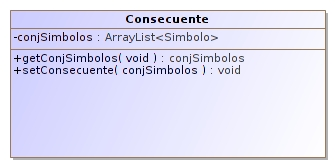
\includegraphics[scale=0.5]{img/clase10.jpg}
	\caption{Representaci�n gr�fica de la clase Consecuente}
	\label{clase10}
      \end{center}
  \end{figure}



\subsection{Clase TablaPredictiva}

Esta clase representa a la tabla Predictiva de una gram�tica de contexto libre. En la tabla \ref{tabla812}
se recoge la especificaci�n de la clase y en la figura \ref{clase12} se muestra su representaci�n gr�fica.

\begin{longtable}[H]{|>{\columncolor[rgb]{0.63,0.79,0.95}}m{6cm} | m{8.5cm} |}
 \caption{Clase TablaPredictiva}

\endfirsthead

\multicolumn{2}{c}
{{\tablename\ \thetable{} -- contin�a de la p�gina anterior}} \\
\endhead

\hline \multicolumn{2}{|r|}{{Contin�a en la p�gina siguiente}} \\ \hline
\endfoot

\hline
\endlastfoot

\hline
 \textbf{Nombre} & \textbf{TablaPredictiva}  \\ \hline
 
 \textbf{Descripci�n} & Representa a la tabla predictiva de una gram�tica de contexto libre.  \\ \hline
                       
 \textbf{Atributos} & \begin{enumerate}
 		\item \textbf{funError}: representa las funciones de tratamiento de errores para completar la tabla 						predictiva.
 		\item \textbf{matrizPred}: este atributo representa la matriz predictiva. La matriz tendr� las siguientes 				dimensiones: [N�mero de s�mbolos no terminales] [N�mero de s�mbolos terminales + 1 (S�mbolo \$)] . Los 				datos dentro de la matriz predictiva pueden ser de dos tipos: 
 			\begin{itemize}
				\item \textit{PN}: producci�n n�mero \textit{N}.
				\item \textit{EN}: funci�n de error n�mero \textit{N}.
			\end{itemize}
 		\end{enumerate}  \\ \hline
 
 \textbf{M�todos} & \begin{enumerate}
 		\item \textbf{construir}: m�todo p�blico que permite construir la tabla Predictiva.
 		\item \textbf{getCeldaPredictiva}: m�todo p�blico que permite obtener una celda de la matriz de la tabla 					predictiva. 		
 		\item \textbf{setCeldaPredictiva}: m�todo p�blico que permite asignar un valor a una celda de la matriz de 				la tabla predictiva.	
 		\item \textbf{crearFunError}: m�todo p�blico que permite crear una nueva funci�n de error.
 		\item \textbf{asignarFuncionError}: m�todo p�blico que permite asignar las funciones de tratamiento de error 			a la tabla.
 		\item \textbf{editarFucionError}: m�todo p�blico que permite editar un funci�n de error.
 		\item \textbf{eliminarFunError}: m�todo p�blico que permite eliminar una funci�n de error ya creada. Si se 				elimina una funci�n que ya est� asignada en la tabla se eliminar� dicha asignaci�n.
\end{enumerate}
                                 
 \label{tabla812}

\end{longtable}

 \begin{figure}[H]
      \begin{center} 
	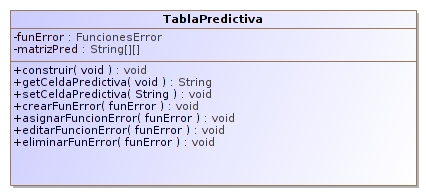
\includegraphics[scale=0.5]{img/clase12.jpg}
	\caption{Representaci�n gr�fica de la clase TablaPredictiva}
	\label{clase12}
      \end{center}
  \end{figure}


\subsection{Clase TablaLR}

Esta clase representa a la tabla LR de una gram�tica de contexto libre. En la tabla \ref{tabla813} se recoge la especificaci�n de la clase y en la figura \ref{clase13} se muestra su representaci�n gr�fica.

\begin{longtable}[H]{|>{\columncolor[rgb]{0.63,0.79,0.95}}m{6cm} | m{8.5cm} |}
 \caption{Clase TablaLR}

\endfirsthead

\multicolumn{2}{c}
{{\tablename\ \thetable{} -- contin�a de la p�gina anterior}} \\
\endhead

\hline \multicolumn{2}{|r|}{{Contin�a en la p�gina siguiente}} \\ \hline
\endfoot

\hline
\endlastfoot

\hline
 \textbf{Nombre} & \textbf{TablaLR}  \\ \hline
 
 \textbf{Descripci�n} & Representa a la tabla LR de una gram�tica de con\-tex\-to libre.  \\ \hline
                       
 \textbf{Atributos} & \begin{enumerate}
	 \item \textbf{metodoAscendente}: este tipo enumerado representa a los m�todos de simulaci�n del 							an�lisis sint�ctico ascendente que pueden ser utilizados en el simulador (SLR, LR, LALR).
	 \item \textbf{TAccion}: este atributo representa a la tabla de la parte acci�n del an�lisis.
	 \item \textbf{TIrA}: este atributo representa a la tabla de la parte ir\_a del an�lisis.
 	
	\end{enumerate} \\ \hline
 
 \textbf{M�todos} & \begin{enumerate}
 	 \item \textbf{getMetodoAsc}: m�todo p�blico que obtiene el valor del m�todo ascendente.
 	 \item \textbf{setMetodoAsc}: m�todo p�blico que permite almacenar el valor del m�todo ascendente.
 	 \item \textbf{generarAccion}: m�todo p�blico que permite construir la parte acci�n de la tabla LR en funci�n 				del m�todo seleccionado.
 	 \item \textbf{getAccion}: m�todo p�blico que permite obtener la matriz acci�n de la gram�tica.
 	 \item \textbf{generarIrA}: m�todo p�blico que permite construir la parte ir\_A de la tabla LR en funci�n 				del m�todo seleccionado.
 	 \item \textbf{getIrA}: m�todo p�blico que permite obtener la matriz Ir\_A de la gram�tica.
	\end{enumerate}
                                 
 \label{tabla813}

\end{longtable}

 \begin{figure}[H]
      \begin{center} 
	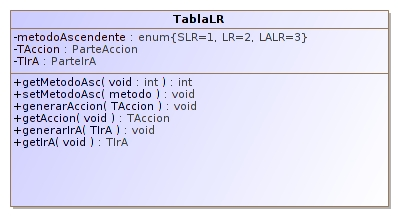
\includegraphics[scale=0.5]{img/clase13.jpg}
	\caption{Representaci�n gr�fica de la clase TablaLR}
	\label{clase13}
      \end{center}
  \end{figure}
  
\subsection{Clase ParteAccion}

Esta clase representa a la parte acci�n de la tabla LR de una gram�tica de contexto libre. En la tabla \ref{tabla819} se recoge la especificaci�n de la clase y en la figura \ref{clase19} se muestra su representaci�n gr�fica.

\begin{longtable}[H]{|>{\columncolor[rgb]{0.63,0.79,0.95}}m{6cm} | m{8.5cm} |}
 \caption{Clase ParteAccion}

\endfirsthead

\multicolumn{2}{c}
{{\tablename\ \thetable{} -- contin�a de la p�gina anterior}} \\
\endhead

\hline \multicolumn{2}{|r|}{{Contin�a en la p�gina siguiente}} \\ \hline
\endfoot

\hline
\endlastfoot

\hline
 \textbf{Nombre} & \textbf{ParteAccion}  \\ \hline
 
 \textbf{Descripci�n} & Representa a la parte acci�n de la tabla LR de una gram�tica de con\-tex\-to libre.  \\ \hline
                       
 \textbf{Atributos} &  \begin{enumerate}
  		\item \textbf{funError}: funciones de tratamiento de errores para completar la tabla predictiva.
 		\item \textbf{matrizAccion}: representa en forma de matriz la parte acci�n de una tabla LR. La matriz tendr� 		la siguiente dimensi�n: [N�mero de estados + 1] [N�mero de s�mbolos terminales + 1 (el s�mbolo \$)]. Los 				datos dentro de la matriz acci�n pueden ser de los siguientes tipos: 
 		\begin{itemize}
			\item \textit{A}: aceptar.
			\item \textit{RN}: reducir con la producci�n n�mero \textit{N}.
			\item \textit{DN}: desplazar y pasar al estado n�mero \textit{N}.
			\item \textit{EN}: funci�n de error n�mero \textit{N}.
		\end{itemize}
					

 		\end{enumerate}  \\ \hline
 
 \textbf{M�todos} & \begin{enumerate} 
 		\item \textbf{construir}: m�todo p�blico que permite construir la matriz de la parte Acci�n.
 		\item \textbf{getCeldaAccion}: m�todo p�blico que permite obtener una celda de la matriz de la parte Acci�n. 
 		
 		\item \textbf{setCeldaAccion}: m�todo p�blico que permite asignar un valor a una celda de la matriz de 				la parte Acci�n.	
 		\item \textbf{crearFunError}: m�todo p�blico que permite crear una nueva funci�n de error.
 		\item \textbf{asignarFuncionError}: m�todo p�blico que permite asignar las funciones de tratamiento de error 			a la tabla.
 		\item \textbf{editarFucionError}: m�todo p�blico que permite editar un funci�n de error.
 		\item \textbf{eliminarFunError}: m�todo p�blico que permite eliminar una funci�n de error ya creada. Si se 				elimina una funci�n que ya est� asignada en la tabla se eliminar� dicha asignaci�n.
\end{enumerate}
                                 
 \label{tabla819}

\end{longtable}

\begin{figure}[H]
      \begin{center} 
	\includegraphics[scale=0.5]{img/clase19.jpg}
	\caption{Representaci�n gr�fica de la clase ParteAccion}
	\label{clase19}
      \end{center}
  \end{figure}


\subsection{Clase ParteIrA}

Esta clase representa a la parte ir a de la tabla LR de una gram�tica de contexto libre. En la tabla \ref{tabla820} se recoge la especificaci�n de la clase y en la figura \ref{clase20} se muestra su representaci�n gr�fica.

\begin{longtable}[H]{|>{\columncolor[rgb]{0.63,0.79,0.95}}m{6cm} | m{8.5cm} |}
 \caption{Clase ParteIrA}

\endfirsthead

\multicolumn{2}{c}
{{\tablename\ \thetable{} -- contin�a de la p�gina anterior}} \\
\endhead

\hline \multicolumn{2}{|r|}{{Contin�a en la p�gina siguiente}} \\ \hline
\endfoot

\hline
\endlastfoot

\hline
 \textbf{Nombre} & \textbf{ParteIrA}  \\ \hline
 
 \textbf{Descripci�n} & Representa a la parte ir a de la tabla LR de una gram�tica de con\-tex\-to libre.  \\ \hline
                       
 \textbf{Atributos} & \begin{enumerate}
		\item \textbf{matrizIrA}: representa en forma de matriz la parte ir\_a de la tabla LR. La matriz tendr� la 				siguiente dimensi�n: [N�mero de estados + 1] [N�mero de simbolos no terminales]. Los datos que 						contiene esta matriz son las transiciones del aut�mata finito determinista (AFD)
\end{enumerate} \\ \hline
 
 \textbf{M�todos} & \begin{enumerate}
		\item \textbf{construir}: m�todo p�blico que permite construir la matriz de la parte Ir\_A.
 		\item \textbf{getCeldaIrA}: m�todo p�blico que permite obtener una celda de la matriz de la parte Acci�n. 
 		\item \textbf{setCeldaIrA}: m�todo p�blico que permite asignar un valor a una celda de la matriz de 					la parte Ir\_A.
		 \end{enumerate}	
                                 
 \label{tabla820}

\end{longtable}

\begin{figure}[H]
      \begin{center} 
	\includegraphics[scale=0.5]{img/clase20.jpg}
	\caption{Representaci�n gr�fica de la clase ParteIrA}
	\label{clase20}
      \end{center}
  \end{figure}

\subsection{Clase FuncionError}

Esta clase representa a las funciones de error utilizadas para completar tanto la tabla predictiva como la tabla LR de una gram�tica de contexto libre. En la tabla \ref{tabla814} se recoge la especificaci�n de la clase y en la figura \ref{clase14} se muestra su representaci�n gr�fica.

\begin{longtable}[H]{|>{\columncolor[rgb]{0.63,0.79,0.95}}m{6cm} | m{8.5cm} |}
 \caption{Clase FuncionError}

\endfirsthead

\multicolumn{2}{c}
{{\tablename\ \thetable{} -- contin�a de la p�gina anterior}} \\
\endhead

\hline \multicolumn{2}{|r|}{{Contin�a en la p�gina siguiente}} \\ \hline
\endfoot

\hline
\endlastfoot

\hline
 \textbf{Nombre} & \textbf{FuncionError}  \\ \hline
 
 \textbf{Descripci�n} & Representa a las funciones de error con las que se completan tanto la tabla 					predictiva como la tabla LR de una gram�tica de con\-tex\-to libre.  \\ \hline
                       
 \textbf{Atributos} & \begin{enumerate}
 		\item \textbf{identificador}: representa al \textit{identificador} de una funci�n de e\-rror.
		 \item \textbf{mensaje}: representa al \textit{mensaje} de una funci�n de e\-rror.
 		\item \textbf{accion}: representa a la \textit{acci�n} que lle\-va a cabo la funci�n de e\-rror. Habr� que 				diferenciar entre la acci�n en las funciones de error en el an�lisis sint�ctico ascendente y 							descendente.
 		\item \textbf{simbolo}: representa al \textit{s�mbolo} que utiliza la funci�n de e\-rror (tanto en la 			entrada como en la pila) o una \textbf{modificaci�n} (tanto en la entrada como en la pila), que 				consistir�a en cambiar un s�mbolo por otro.

	\end{enumerate} \\ \hline
 
 \textbf{M�todos} & \begin{enumerate}
 		\item \textbf{getIdentificador}: m�todo p�blico que permite obtener el identificador de la funci�n de error. 
 		\item \textbf{setIdentificador}: m�todo p�blico que permite asignar el identificador a la funci�n de error.
 		\item \textbf{getMensaje}: m�todo p�blico que permite obtener el mensaje	de la funci�n de error. 
	 	\item \textbf{setMensaje}: m�todo p�blico que permite asignar el mensaje a la funci�n de error.
	 	\item \textbf{getAccion}: m�todo p�blico que permite obtener la acci�n que lleva a cabo la funci�n de error.
 		\item \textbf{setAccion}: m�todo p�blico que permite asignar la accion a 	la funci�n de error.
		\item \textbf{getSimbolo}:m�todo p�blico que permite obtener el simbolo que utiliza la funci�n de error (en 				caso de que utilice alguno).
 		\item \textbf{setSimbolo}: m�todo p�blico que permite asignar el simbolo a la funci�n de error.

\end{enumerate}
                             
 \label{tabla814}

\end{longtable}

 \begin{figure}[H]
      \begin{center} 
	\includegraphics[scale=0.5]{img/clase14.jpg}
	\caption{Representaci�n gr�fica de la clase FuncionError}
	\label{clase14}
      \end{center}
  \end{figure}
  
\subsection{ColCanLR(0)}

Esta clase representa a la colecci�n can�nica de elementos LR(0) necesaria para llevar a cabo el an�lisis sint�ctico ascendente SLR. En la tabla \ref{tabla822} se recoge la especificaci�n de la clase y en la figura \ref{clase22} se muestra su representaci�n gr�fica.


\begin{longtable}[H]{|>{\columncolor[rgb]{0.63,0.79,0.95}}m{6cm} | m{8.5cm} |}
 \caption{Clase ColCanLR(0)}

\endfirsthead

\multicolumn{2}{c}
{{\tablename\ \thetable{} -- contin�a de la p�gina anterior}} \\
\endhead

\hline \multicolumn{2}{|r|}{{Contin�a en la p�gina siguiente}} \\ \hline
\endfoot

\hline
\endlastfoot

\hline
 \textbf{Nombre} & \textbf{ColCanLR(0)}  \\ \hline
 
 \textbf{Descripci�n} & Representa a colecci�n can�nica de elementos LR(0) necesaria en el an�lisis sint�ctica ascendente SLR.  \\ \hline
                       
 \textbf{Atributos} & \begin{enumerate}
 		
 		\item \textbf{conjElementosLR0}: este atributo representa el conjunto de elementos LR(0) en el an�lisis sint�ctico ascendente SLR.

	\end{enumerate} \\ \hline
 
 \textbf{M�todos} & \begin{enumerate}
 		\item \textbf{getConjElementosLR0}: m�todo p�blico que permite obtener el conjunto de elementos LR(0).
 		\item \textbf{setConjElementosLR0}: m�todo p�blico que permite asignar el valor al conjunto de elementos 					LR(0).

\end{enumerate}
                             
 \label{tabla822}

\end{longtable}

 \begin{figure}[H]
      \begin{center} 
	\includegraphics[scale=0.5]{img/clase22.jpg}
	\caption{Representaci�n gr�fica de la clase ColCanLR(0)}
	\label{clase22}
      \end{center}
  \end{figure}

\subsection{ColCanLR(1)}

Esta clase representa a la colecci�n can�nica de elementos LR(1) necesaria para llevar a cabo el an�lisis sint�ctico ascendente LR-can�nico. En la tabla \ref{tabla823} se recoge la especificaci�n de la clase y en la figura \ref{clase823} se muestra su representaci�n gr�fica.

\begin{longtable}[H]{|>{\columncolor[rgb]{0.63,0.79,0.95}}m{6cm} | m{8.5cm} |}
 \caption{Clase ColCanLR(1)}

\endfirsthead

\multicolumn{2}{c}
{{\tablename\ \thetable{} -- contin�a de la p�gina anterior}} \\
\endhead

\hline \multicolumn{2}{|r|}{{Contin�a en la p�gina siguiente}} \\ \hline
\endfoot

\hline
\endlastfoot

\hline
 \textbf{Nombre} & \textbf{ColCanLR(1)}  \\ \hline
 
 \textbf{Descripci�n} & Representa a colecci�n can�nica de elementos LR(1) necesaria en el an�lisis sint�ctica ascendente LR-can�nico.  \\ \hline
                       
 \textbf{Atributos} & \begin{enumerate}
 		
 		\item \textbf{conjElementosLR1}: este atributo representa el conjunto de elementos LR(1) en el an�lisis 					sint�ctico ascendente LR-can�nico.

	\end{enumerate} \\ \hline
 
 \textbf{M�todos} & \begin{enumerate}
 		\item \textbf{getConjElementosLR1}: m�todo p�blico que permite obtener el conjunto de elementos LR(1).
 		\item \textbf{setConjElementosLR1}: m�todo p�blico que permite asignar el valor al conjunto de elementos 					LR(1).
\end{enumerate}
                             
 \label{tabla823}

\end{longtable}

 \begin{figure}[H]
      \begin{center} 
	\includegraphics[scale=0.5]{img/clase23.jpg}
	\caption{Representaci�n gr�fica de la clase ColCanLR(1)}
	\label{clase823}
      \end{center}
  \end{figure}


\subsection{ColCanLALR(1)}

Esta clase representa a la colecci�n can�nica de elementos LALR(1) necesaria para llevar a cabo el an�lisis sint�ctico ascendente LALR. En la tabla \ref{tabla824} se recoge la especificaci�n de la clase y en la figura \ref{clase824} se muestra su representaci�n gr�fica.


\begin{longtable}[H]{|>{\columncolor[rgb]{0.63,0.79,0.95}}m{6cm} | m{8.5cm} |}
 \caption{Clase ColCanLALR(1)}

\endfirsthead

\multicolumn{2}{c}
{{\tablename\ \thetable{} -- contin�a de la p�gina anterior}} \\
\endhead

\hline \multicolumn{2}{|r|}{{Contin�a en la p�gina siguiente}} \\ \hline
\endfoot

\hline
\endlastfoot

\hline
 \textbf{Nombre} & \textbf{ColCanLALR(1)}  \\ \hline
 
 \textbf{Descripci�n} & Representa a colecci�n can�nica de elementos LALR(1) necesaria en el an�lisis sint�ctica ascendente LALR.  \\ \hline
                       
 \textbf{Atributos} & \begin{enumerate}
 		
 		\item \textbf{conjElementosLALR1}: este atributo representa el conjunto de elementos LALR(1) en el an�lisis 				sint�ctico ascendente LALR.

	\end{enumerate} \\ \hline
 
 \textbf{M�todos} & \begin{enumerate}
 		\item \textbf{getConjElementosLALR1}: m�todo p�blico que permite obtener el conjunto de elementos LALR(1).
 		\item \textbf{setConjElementosLALR1}: m�todo p�blico que permite asignar el valor al conjunto de elementos 				LALR(1).

\end{enumerate}
                             
 \label{tabla824}

\end{longtable}

 \begin{figure}[H]
      \begin{center} 
	\includegraphics[scale=0.5]{img/clase24.jpg}
	\caption{Representaci�n gr�fica de la clase ColCanLALR(1)}
	\label{clase824}
      \end{center}
  \end{figure}

\subsection{ConjElementosLR(0)}

Esta clase representa al conjunto de elementos LR(0) necesaria para llevar a cabo el an�lisis sint�ctico ascendente SLR. En la tabla \ref{tabla825} se recoge la especificaci�n de la clase y en la figura \ref{clase825} se muestra su representaci�n gr�fica.

\begin{longtable}[H]{|>{\columncolor[rgb]{0.63,0.79,0.95}}m{6cm} | m{8.5cm} |}
 \caption{Clase ConjElementosLR(0)}

\endfirsthead

\multicolumn{2}{c}
{{\tablename\ \thetable{} -- contin�a de la p�gina anterior}} \\
\endhead

\hline \multicolumn{2}{|r|}{{Contin�a en la p�gina siguiente}} \\ \hline
\endfoot

\hline
\endlastfoot

\hline
 \textbf{Nombre} & \textbf{ConjElementosLR(0)}  \\ \hline
 
 \textbf{Descripci�n} & Representa al conjunto de elementos LR(0) necesaria en el an�lisis sint�ctica ascendente SLR.  \\ \hline
                       
 \textbf{Atributos} & \begin{enumerate}
 		\item \textbf{elementosLR0}: este atributo representa al conjunto de todos los elementos LR(0) de la 						gram�tica. Se utiliza en el an�lisis sint�ctico SLR. 
 \end{enumerate}\\ \hline
 
 \textbf{M�todos} & \begin{enumerate}
 		\item \textbf{getElementosLR0}: m�todo p�blico que permite obtener los elementos LR(0).
 		\item \textbf{setElementosLR0}: m�todo p�blico que permite asignar el valor al conjunto de elementos LR(0).


\end{enumerate}
                             
 \label{tabla825}

\end{longtable}

 \begin{figure}[H]
      \begin{center} 
	\includegraphics[scale=0.5]{img/clase25.jpg}
	\caption{Representaci�n gr�fica de la clase ConjElementosLR(0)}
	\label{clase825}
      \end{center}
  \end{figure}

\subsection{ConjElementosLR(1)}

Esta clase representa al conjunto de elementos LR(1) necesaria para llevar a cabo el an�lisis sint�ctico ascendente LR-can�nico. En la tabla \ref{tabla826} se recoge la especificaci�n de la clase y en la figura \ref{clase826} se muestra su representaci�n gr�fica.


\begin{longtable}[H]{|>{\columncolor[rgb]{0.63,0.79,0.95}}m{6cm} | m{8.5cm} |}
 \caption{Clase ConjElementosLR(1)}

\endfirsthead

\multicolumn{2}{c}
{{\tablename\ \thetable{} -- contin�a de la p�gina anterior}} \\
\endhead

\hline \multicolumn{2}{|r|}{{Contin�a en la p�gina siguiente}} \\ \hline
\endfoot

\hline
\endlastfoot

\hline
 \textbf{Nombre} & \textbf{ConjElementosLR(1)}  \\ \hline
 
 \textbf{Descripci�n} & Representa al conjunto de elementos LR(1) necesaria en el an�lisis sint�ctica ascendente LR-can�nico.  \\ \hline
                       
 \textbf{Atributos} & \begin{enumerate}
 		\item \textbf{elementosLR1}: este atributo representa al conjunto de todos los elementos LR(1) de la 						gram�tica. Se utiliza en el an�lisis sint�ctico LR-can�nico.

	\end{enumerate} \\ \hline
 
 \textbf{M�todos} & \begin{enumerate}
 		\item \textbf{getElementosLR1}: m�todo p�blico que permite obtener los elementos LR(1).
 		\item \textbf{setElementosLR1}: m�todo p�blico que permite asignar el valor a los elementos LR(1).

\end{enumerate}
                             
 \label{tabla826}

\end{longtable}

 \begin{figure}[H]
      \begin{center} 
	\includegraphics[scale=0.5]{img/clase26.jpg}
	\caption{Representaci�n gr�fica de la clase ConjElementosLR(1)}
	\label{clase826}
      \end{center}
  \end{figure}

\subsection{ConjElementosLARL(1)}

Esta clase representa al conjunto de elementos LALR(1) necesaria para llevar a cabo el an�lisis sint�ctico ascendente LALR. En la tabla \ref{tabla827} se recoge la especificaci�n de la clase y en la figura \ref{clase827} se muestra su representaci�n gr�fica.


\begin{longtable}[H]{|>{\columncolor[rgb]{0.63,0.79,0.95}}m{6cm} | m{8.5cm} |}
 \caption{Clase ConjElementosLALR(1)}

\endfirsthead

\multicolumn{2}{c}
{{\tablename\ \thetable{} -- contin�a de la p�gina anterior}} \\
\endhead

\hline \multicolumn{2}{|r|}{{Contin�a en la p�gina siguiente}} \\ \hline
\endfoot

\hline
\endlastfoot

\hline
 \textbf{Nombre} & \textbf{ConjElementosLALR(1)}  \\ \hline
 
 \textbf{Descripci�n} & Representa al conjunto de elementos LALR(1) necesaria en el an�lisis sint�ctica ascendente LALR.  \\ \hline
                       
 \textbf{Atributos} & \begin{enumerate}
 		\item \textbf{elementosLALR1}: este atributo representa al conjunto de todos los elementos LALR(1) de la 						gram�tica. Se utiliza en el an�lisis sint�ctico LALR.

	\end{enumerate} \\ \hline
 
 \textbf{M�todos} & \begin{enumerate}
 		\item \textbf{getElementosLALR1}: m�todo p�blico que permite obtener los elementos LALR(1).
 		\item \textbf{setElementosLALR1}: m�todo p�blico que permite asignar el valor a los elementos LALR(1).

\end{enumerate}
                             
 \label{tabla827}

\end{longtable}

 \begin{figure}[H]
      \begin{center} 
	\includegraphics[scale=0.5]{img/clase27.jpg}
	\caption{Representaci�n gr�fica de la clase ConjElementosLALR(1)}
	\label{clase827}
      \end{center}
  \end{figure}

\subsection{ElementosLR(0)}

Esta clase representa al elemento LR(0) necesaria para llevar a cabo el an�lisis sint�ctico ascendente SLR. En la tabla \ref{tabla828} se recoge la especificaci�n de la clase y en la figura \ref{clase828} se muestra su representaci�n gr�fica.


\begin{longtable}[H]{|>{\columncolor[rgb]{0.63,0.79,0.95}}m{6cm} | m{8.5cm} |}
 \caption{Clase ElementosLR(0)}

\endfirsthead

\multicolumn{2}{c}
{{\tablename\ \thetable{} -- contin�a de la p�gina anterior}} \\
\endhead

\hline \multicolumn{2}{|r|}{{Contin�a en la p�gina siguiente}} \\ \hline
\endfoot

\hline
\endlastfoot

\hline
 \textbf{Nombre} & \textbf{ElementosLR(0)}  \\ \hline
 
 \textbf{Descripci�n} & Representa al elemento LR(0) necesario en el an�lisis sint�ctica ascendente SLR.  \\ \hline
                       
 \textbf{Atributos} & \begin{enumerate}
 
		\item  \textbf{produc}: este atributo representa el n�mero de la producci�n que se est� utilizando para la 				obtenci�n de los elementos LR(0).
		\item \textbf{posicion}: este atributo representa la posici�n del punto en la parte derecha de la producci�n 			que se est� utilizando.
 \end{enumerate}\\ \hline
 
 \textbf{M�todos} & \begin{enumerate}
 		\item \textbf{getProduc}: m�todo p�blico que permite obtener el n�mero de la producci�n.
 		\item \textbf{setProduc}: m�todo p�blico que permite asignar el valor del n�mero de la producci�n que se 					est� utilizando.
 		\item \textbf{getPosicion}: m�todo p�blico que permite obtener la posici�n del punto dentro de la parte 					derecha de una producci�n.
 		\item \textbf{setPosicion}: m�todo p�blico que permite asignar el valor de la posici�n del punto en la parte 			derecha 	de una producci�n.

\end{enumerate}
                             
 \label{tabla828}

\end{longtable}

 \begin{figure}[H]
      \begin{center} 
	\includegraphics[scale=0.5]{img/clase28.jpg}
	\caption{Representaci�n gr�fica de la clase ElementosLR(0)}
	\label{clase828}
      \end{center}
  \end{figure}

\subsection{ElementosLR(1)}

Esta clase representa al elemento LR(1) necesaria para llevar a cabo el an�lisis sint�ctico ascendente LR-can�nico. En la tabla \ref{tabla829} se recoge la especificaci�n de la clase y en la figura \ref{clase829} se muestra su representaci�n gr�fica.


\begin{longtable}[H]{|>{\columncolor[rgb]{0.63,0.79,0.95}}m{6cm} | m{8.5cm} |}
 \caption{Clase ElementosLR(1)}

\endfirsthead

\multicolumn{2}{c}
{{\tablename\ \thetable{} -- contin�a de la p�gina anterior}} \\
\endhead

\hline \multicolumn{2}{|r|}{{Contin�a en la p�gina siguiente}} \\ \hline
\endfoot

\hline
\endlastfoot

\hline
 \textbf{Nombre} & \textbf{ElementosLR(1)}  \\ \hline
 
 \textbf{Descripci�n} & Representa al elemento LR(1) necesaria en el an�lisis sint�ctica ascendente LR-can�nico.  \\ \hline
                       
 \textbf{Atributos} & \begin{enumerate}
 		\item  \textbf{produc}: este atributo representa el n�mero de la producci�n que se est� utilizando para la 				obtenci�n de los elementos LR(1).
		\item \textbf{posicion}: este atributo representa la posici�n del punto en la parte derecha de la producci�n 			que se est� utilizando.
		\item \textbf{anticipacion}: este atributo representa al s�mbolo de anticipaci�n que es un s�mbolo no 					terminal o el s�mbolo \$.

	\end{enumerate} \\ \hline
 
 \textbf{M�todos} & \begin{enumerate}
 		\item \textbf{getProduc}: m�todo p�blico que permite obtener el n�mero de la producci�n.
 		\item \textbf{setProduc}: m�todo p�blico que permite asignar el valor del n�mero de la producci�n que se 					est� utilizando.
 		\item \textbf{getPosicion}: m�todo p�blico que permite obtener la posici�n del punto dentro de la parte 					derecha de una producci�n.
 		\item \textbf{setPosicion}: m�todo p�blico que permite asignar el valor de la posici�n del punto en la parte 			derecha 	de una producci�n.
 		\item \textbf{getAnticipacion}: m�todo p�blico que permite obtener el s�mbolo de anticipaci�n.
 		\item \textbf{setAnticipacion}: m�todo p�blico que permite asignar el valor al s�mbolo de anticipaci�n.
 		

\end{enumerate}
                             
 \label{tabla829}

\end{longtable}

 \begin{figure}[H]
      \begin{center} 
	\includegraphics[scale=0.5]{img/clase29.jpg}
	\caption{Representaci�n gr�fica de la clase ElementosLR(1)}
	\label{clase829}
      \end{center}
  \end{figure}
\newpage
\subsection{ElementosLALR(1)}

Esta clase representa al elemento LALR(1) necesaria para llevar a cabo el an�lisis sint�ctico ascendente LALR. En la tabla \ref{tabla830} se recoge la especificaci�n de la clase y en la figura \ref{clase830} se muestra su representaci�n gr�fica.


\begin{longtable}[H]{|>{\columncolor[rgb]{0.63,0.79,0.95}}m{6cm} | m{8.5cm} |}
 \caption{Clase ElementosLALR(1)}

\endfirsthead

\multicolumn{2}{c}
{{\tablename\ \thetable{} -- contin�a de la p�gina anterior}} \\
\endhead

\hline \multicolumn{2}{|r|}{{Contin�a en la p�gina siguiente}} \\ \hline
\endfoot

\hline
\endlastfoot

\hline
 \textbf{Nombre} & \textbf{ElementosLALR(1)}  \\ \hline
 
 \textbf{Descripci�n} & Representa al elemento LALR(1) necesaria en el an�lisis sint�ctica ascendente LALR.  \\ \hline
                       
  \textbf{Atributos} & \begin{enumerate}
 		\item  \textbf{produc}: este atributo representa el n�mero de la producci�n que se est� utilizando para la 				obtenci�n de los elementos LALR(1).
		\item \textbf{posicion}: este atributo representa la posici�n del punto en la parte derecha de la producci�n 			que se est� utilizando.
		\item \textbf{anticipacion}: este atributo representa al s�mbolo de anticipaci�n que es un s�mbolo no 					terminal o el s�mbolo \$.

	\end{enumerate} \\ \hline
 
 \textbf{M�todos} & \begin{enumerate}
 		\item \textbf{getProduc}: m�todo p�blico que permite obtener el n�mero de la producci�n.
 		\item \textbf{setProduc}: m�todo p�blico que permite asignar el valor del n�mero de la producci�n que se 					est� utilizando.
 		\item \textbf{getPosicion}: m�todo p�blico que permite obtener la posici�n del punto dentro de la parte 					derecha de una producci�n.
 		\item \textbf{setPosicion}: m�todo p�blico que permite asignar el valor de la posici�n del punto en la parte 			derecha 	de una producci�n.
 		\item \textbf{getAnticipacion}: m�todo p�blico que permite obtener el s�mbolo de anticipaci�n.
 		\item \textbf{setAnticipacion}: m�todo p�blico que permite asignar el valor al s�mbolo de anticipaci�n.
 		
\end{enumerate}
                             
 \label{tabla830}

\end{longtable}

 \begin{figure}[H]
      \begin{center} 
	\includegraphics[scale=0.5]{img/clase30.jpg}
	\caption{Representaci�n gr�fica de la clase ElementosLALR(1)}
	\label{clase830}
      \end{center}
  \end{figure}
  
\subsection{Clase Simulador}

Esta clase representa al simulador de gram�ticas de contexto libre. En la tabla \ref{tabla811}
se recoge la especificaci�n de la clase y en la figura \ref{clase11} se muestra su representaci�n gr�fica.

\begin{longtable}[H]{|>{\columncolor[rgb]{0.63,0.79,0.95}}m{6cm} | m{8.5cm} |}
 \caption{Clase Simulador}

\endfirsthead

\multicolumn{2}{c}
{{\tablename\ \thetable{} -- contin�a de la p�gina anterior}} \\
\endhead

\hline \multicolumn{2}{|r|}{{Contin�a en la p�gina siguiente}} \\ \hline
\endfoot

\hline
\endlastfoot

\hline
 \textbf{Nombre} & \textbf{Simulador}  \\ \hline
 
 \textbf{Descripci�n} & Representa a un simulador de gram�ticas de contexto libre.  \\ \hline
                       
 \textbf{Atributos} & \begin{enumerate}
		 \item \textbf{cadenaEntrada}: representa a la cadena de entrada, que estar� compuesta por s�mbolos 			terminales y se usar� para ver si es reconocida o no durante la simulaci�n.
		 \item \textbf{metodoSimulacion}: tipo enumerado que representa los dos tipos de simulaciones que se 						pueden llevar a cabo: m�todo Descendente y m�todo Ascendente.
 		\item \textbf{modoFuncionamiento}: este tipo enumerado representa a la velocidad de funcionamiento del 					si\-mu\-la\-dor (paso a paso o cont�nuo).
 		
	\end{enumerate}\\ \hline
 
 \textbf{M�todos} & \begin{enumerate}
 		\item \textbf{cargarGramatica}: m�todo p�blico que permite seleccionar la gram�tica a ser simulada.
 		\item \textbf{getMetodoSim}: m�todo p�blico que permite obtener el m�todo de simulaci�n, 1 si es el m�todo 				descendente y 2 si es el m�todo ascendente.
 		\item \textbf{setMetodoSim}: m�todo p�blico que permite almacenar el valor del m�todo de simulaci�n, 1 si es 			el m�todo descendente y 2 si es el m�todo ascendente. 
 		\item \textbf{getModoFunc}: m�todo p�blico que permite obtener el modo de funcionamiento del simulaci�n, 1 				si es el modo cont�nuo y 2 si es el modo paso a paso.
 		\item \textbf{setModoFunc}: m�todo p�blico que permite almacenar el valor del modo de funcionamiento del 					simulaci�n, 1 si es el modo cont�nuo y 2 si es el modo paso a paso.
 		\item \textbf{lanzarSimulador}: m�todo privado que permite lanzar el simulador en funci�n del m�todo de 					funcionamiento y m�todo de simulaci�n seleccionado.  
 		\item \textbf{generarInforme}: m�todo p�blico que permite obtener el informe de la simulaci�n en formato 					PDF.
	\end{enumerate}
                                 
 \label{tabla811}

\end{longtable}

 \begin{figure}[H]
      \begin{center} 
	\includegraphics[scale=0.5]{img/clase11.jpg}
	\caption{Representaci�n gr�fica de la clase Simulador}
	\label{clase11}
      \end{center}
  \end{figure}
  
  
\subsection{Clase CadenaEntrada}

Esta clase representa a la cadena de entrada en la simulaci�n de una gram�tica de contexto libre. En la tabla \ref{tabla821} se recoge la especificaci�n de la clase y en la figura \ref{clase21} se muestra su representaci�n gr�fica.

\begin{longtable}[H]{|>{\columncolor[rgb]{0.63,0.79,0.95}}m{6cm} | m{8.5cm} |}
 \caption{Clase CadenaEntrada}

\endfirsthead

\multicolumn{2}{c}
{{\tablename\ \thetable{} -- contin�a de la p�gina anterior}} \\
\endhead

\hline \multicolumn{2}{|r|}{{Contin�a en la p�gina siguiente}} \\ \hline
\endfoot

\hline
\endlastfoot

\hline
 \textbf{Nombre} & \textbf{CadenaEntrada}  \\ \hline
 
 \textbf{Descripci�n} & Representa la cadena de entrada en la simulaci�n de una gram�tica de con\-tex\-to libre.  \\ \hline
                       
 \textbf{Atributos} & \begin{enumerate}
 		\item \textbf{cadena}: conjunto de s�mbolos terminales que forman parte de la cadena de entrada.
 \end{enumerate} \\ \hline 
 
 \textbf{M�todos} &  \begin{enumerate}
 		\item \textbf{getCadena}: m�todo p�blico que recoge la cadena de entrada.
 		\item \textbf{setCadena}: m�todo p�blico que modifica el valor de la cadena de entrada.
 \end{enumerate}
                                 
 \label{tabla821}

\end{longtable}

 \begin{figure}[H]
      \begin{center} 
	\includegraphics[scale=0.5]{img/clase21.jpg}
	\caption{Representaci�n gr�fica de la clase CadenaEntrada}
	\label{clase21}
      \end{center}
  \end{figure}


\subsection{Clase Ayuda}

Esta clase representa a la ayuda de la aplicaci�n. En la tabla \ref{tabla815} se recoge la especificaci�n de la clase y en la figura \ref{clase15} se muestra su representaci�n gr�fica.

\begin{longtable}[H]{|>{\columncolor[rgb]{0.63,0.79,0.95}}m{6cm} | m{8.5cm} |}
 \caption{Clase Ayuda}

\endfirsthead

\multicolumn{2}{c}
{{\tablename\ \thetable{} -- contin�a de la p�gina anterior}} \\
\endhead

\hline \multicolumn{2}{|r|}{{Contin�a en la p�gina siguiente}} \\ \hline
\endfoot

\hline
\endlastfoot

\hline
 \textbf{Nombre} & \textbf{Ayuda}  \\ \hline
 
 \textbf{Descripci�n} & Representa a la ayuda de la aplicaci�n.  \\ \hline
                       
 \textbf{Atributos} & \begin{enumerate}
 		\item \textbf{capitulos}: contiene el \textit{conjunto de cap�tulos} que forman la ayuda.
	\end{enumerate} \\ \hline
 
 \textbf{M�todos} & \begin{enumerate}
 		\item \textbf{inicializarAyuda}: m�todo p�blico que permite inicializar la ayuda. Es utilizado tanto por el 				editor como por el simulador.
 		\item \textbf{buscarCapitulo}: m�todo p�blico que permite buscar un cap�tulo de la ayuda y recuperarlo.
 		\item \textbf{visualizarCapitulo}: m�todo p�blico que permite visualizar un cap�tulo de la ayuda.
	\end{enumerate}
                             
 \label{tabla815}

\end{longtable}

 \begin{figure}[H]
      \begin{center} 
	\includegraphics[scale=0.5]{img/clase15.jpg}
	\caption{Representaci�n gr�fica de la clase Ayuda}
	\label{clase15}
      \end{center}
  \end{figure}

\subsection{Clase Capitulo}

Esta clase representa a los cap�tulos de la ayuda de la aplicaci�n. En la tabla \ref{tabla816} se recoge la especificaci�n de la clase y en la figura \ref{clase16} se muestra su representaci�n gr�fica.

\begin{longtable}[H]{|>{\columncolor[rgb]{0.63,0.79,0.95}}m{6cm} | m{8.5cm} |}
 \caption{Clase Capitulo}

\endfirsthead

\multicolumn{2}{c}
{{\tablename\ \thetable{} -- contin�a de la p�gina anterior}} \\
\endhead

\hline \multicolumn{2}{|r|}{{Contin�a en la p�gina siguiente}} \\ \hline
\endfoot

\hline
\endlastfoot

\hline
 \textbf{Nombre} & \textbf{Capitulo}  \\ \hline
 
 \textbf{Descripci�n} & Representa a los cap�tulos de la ayuda de la aplicaci�n.  \\ \hline
                       
 \textbf{Atributos} & \begin{enumerate}
 		\item \textbf{contenido}: \textit{contenido HTML} del cap�tulo.
		\end{enumerate} \\ \hline
 
 \textbf{M�todos} & \begin{enumerate}
 		\item \textbf{obtenerContenidoHTML}: m�todo p�blico que devuelve el contenido HTML del cap�tulo. Es 						utilizado por el m�dulo de la ayuda, para visualizar los cap�tulos de la misma.
	\end{enumerate}
                             
 \label{tabla816}

\end{longtable}

 \begin{figure}[H]
      \begin{center} 
	\includegraphics[scale=0.5]{img/clase16.jpg}
	\caption{Representaci�n gr�fica de la clase Capitulo}
	\label{clase16}
      \end{center}
  \end{figure}

\subsection{Clase Tutorial}

Esta clase representa al tutorial de la aplicaci�n. En la tabla \ref{tabla817} se recoge la especificaci�n de la clase y en la figura \ref{clase17} se muestra su representaci�n gr�fica.

\begin{longtable}[H]{|>{\columncolor[rgb]{0.63,0.79,0.95}}m{6cm} | m{8.5cm} |}
 \caption{Clase Tutorial}

\endfirsthead

\multicolumn{2}{c}
{{\tablename\ \thetable{} -- contin�a de la p�gina anterior}} \\
\endhead

\hline \multicolumn{2}{|r|}{{Contin�a en la p�gina siguiente}} \\ \hline
\endfoot

\hline
\endlastfoot

\hline
 \textbf{Nombre} & \textbf{Tutorial}  \\ \hline
 
 \textbf{Descripci�n} & Representa al tutorial de la aplicaci�n.  \\ \hline
                       
 \textbf{Atributos} & \begin{enumerate}
 		\item \textbf{lecciones}: lista de las lecciones del tutorial.
		\end{enumerate} \\ \hline
 
 \textbf{M�todos} & \begin{enumerate}
 		\item \textbf{visualizarLeccion}: m�todo p�blico que permite visualizar un lecci�n del tutorial.
	\end{enumerate}
                             
 \label{tabla817}

\end{longtable}

\begin{figure}[H]
      \begin{center} 
	\includegraphics[scale=0.5]{img/clase17.jpg}
	\caption{Representaci�n gr�fica de la clase Tutorial}
	\label{clase17}
      \end{center}
  \end{figure}


\subsection{Clase Leccion}

Esta clase representa a las lecciones del tutorial de la aplicaci�n. En la tabla \ref{tabla818} se recoge la especificaci�n de la clase y en la figura \ref{clase18} se muestra su representaci�n gr�fica.

\begin{longtable}[H]{|>{\columncolor[rgb]{0.63,0.79,0.95}}m{6cm} | m{8.5cm} |}
 \caption{Clase Leccion}

\endfirsthead

\multicolumn{2}{c}
{{\tablename\ \thetable{} -- contin�a de la p�gina anterior}} \\
\endhead

\hline \multicolumn{2}{|r|}{{Contin�a en la p�gina siguiente}} \\ \hline
\endfoot

\hline
\endlastfoot

\hline
 \textbf{Nombre} & \textbf{Leccion}  \\ \hline
 
 \textbf{Descripci�n} & Representa a las lecciones del tutorial de la aplicaci�n.  \\ \hline
                       
 \textbf{Atributos} & \begin{enumerate}
 		\item \textbf{contenido}: contenido pdf de la lecci�n.
		\end{enumerate} \\ \hline
 
 \textbf{M�todos} & \begin{enumerate}
 		\item \textbf{obtenerContenidoPDF}: m�todo p�blico que permite obtener el contenido PDF del la lecci�n. 
	\end{enumerate}
                             
 \label{tabla818}

\end{longtable}

\begin{figure}[H]
      \begin{center} 
	\includegraphics[scale=0.5]{img/clase18.jpg}
	\caption{Representaci�n gr�fica de la clase Leccion}
	\label{clase18}
      \end{center}
  \end{figure}
\newpage

\section{Relaciones entre las clases}

En esta secci�n se rea\-li\-za\-r� un an�lisis de las relaciones existentes entre cada una de las clases analizadas anteriormente.

\subsection{Componentes del sistema}

Representa la relaci�n de composici�n existente entre la clase principal de la aplicaci�n, \textbf{SimAS} y las clases que representan a los componentes principales de la misma que son \textbf{Editor}, \textbf{Simulador}, \textbf{Ayuda} y \textbf{Tutorial}. En la figura \ref{rel1} se muestra la representaci�n gr�fica de esta relaci�n.

 \begin{figure}[H]
      \begin{center} 
	\includegraphics[scale=0.5]{img/rel1.jpg}
	\caption{Relaci�n de los componentes del Sistema}
	\label{rel1}
      \end{center}
  \end{figure}

\subsection{Relaci�n Editor - Gram�tica}

Representa la relaci�n de uso existente entre el \textbf{editor} y la \textbf{gram�tica} de contexto libre, en las que el editor puede utilizar una gram�ticas. En la figura \ref{rel2} se muestra la representaci�n gr�fica de esta relaci�n.

 \begin{figure}[H]
      \begin{center} 
	\includegraphics[scale=0.5]{img/rel2.jpg}
	\caption{Relaci�n Editor-Gramatica}
	\label{rel2}
      \end{center}
  \end{figure}


\subsection{Relaci�n Simulador - Gram�tica}

Representa la relaci�n de uso existente entre el \textbf{si\-mu\-la\-dor} y la \textbf{gram�tica} de contexto libre, en las que el si\-mu\-la\-dor puede utilizar una gram�tica. En la figura \ref{rel3} se muestra la representaci�n gr�fica de esta relaci�n.

\begin{figure}[H]
      \begin{center} 
	\includegraphics[scale=0.5]{img/rel3.jpg}
	\caption{Relaci�n Simulador-Gramatica}
	\label{rel3}
      \end{center}
  \end{figure}

\subsection{Relaci�n Ayuda - Capitulo}

Representa la relaci�n de composici�n existente entre la \textbf{ayuda} del simulador y los \textbf{cap�tulos}, que representa el hecho de que la ayuda se compone de uno o varios cap�tulos. En la figura \ref{rel4} se muestra la representaci�n gr�fica de esta relaci�n.

\begin{figure}[H]
      \begin{center} 
	\includegraphics[scale=0.5]{img/rel4.jpg}
	\caption{Relaci�n Ayuda-Capitulo}
	\label{rel4}
      \end{center}
  \end{figure}

\subsection{Relaci�n Tutorial - Leccion}

Representa la relaci�n de composici�n existente entre el \textbf{tutorial} del simulador y las \textbf{lecciones}, que representa el hecho de que el tutorial se compone de una o varias lecciones. En la figura \ref{rel5} se muestra la representaci�n gr�fica de esta relaci�n.

\begin{figure}[H]
      \begin{center} 
	\includegraphics[scale=0.5]{img/rel5.jpg}
	\caption{Relaci�n Tutorial-Leccion}
	\label{rel5}
      \end{center}
  \end{figure}

\subsection{Componentes de la gram�tica}

Representa la relaci�n de composici�n existente entre la \textbf{gram�tica} y sus componentes (\textbf{produccion}, \textbf{NoTerminal} y \textbf{Terminal}). La gram�tica se compone de varias producciones, de uno o varios s�mbolos no terminales y uno o varios s�mbolos terminales. En la figura \ref{rel6} se muestra la representaci�n gr�fica de esta relaci�n.

\begin{figure}[H]
      \begin{center} 
	\includegraphics[scale=0.5]{img/rel6.jpg}
	\caption{Relaci�n componentes de la Gramatica}
	\label{rel6}
      \end{center}
  \end{figure}
  
\subsection{Gramatica - TablaPredictiva}

Representa la relaci�n existente entre la \textbf{gram�tica} y la \textbf{tabla predictiva}, de forma que de una gram�tica se puede obtener ninguna o una tabla predictiva, mientras que una tabla predictiva solamente puede pertenecer a una �nica gram�tica. En la figura \ref{rel7} se muestra la representaci�n gr�fica de esta relaci�n.

\begin{figure}[H]
      \begin{center} 
	\includegraphics[scale=0.5]{img/rel7.jpg}
	\caption{Relaci�n Gramatica-TablaPredictiva}
	\label{rel7}
      \end{center}
  \end{figure}

\subsection{Gramatica - TablaLR}

Representa la relaci�n existente entre la \textbf{gram�tica} y la \textbf{tabla LR}, de forma que de una gram�tica se puede obtener ninguna o tres tablas LR (una por cada m�todo de an�lisis sint�ctico ascendente), mientras que una tabla LR solamente puede pertenecer a una �nica gram�tica. En la figura \ref{rel8} se muestra la representaci�n gr�fica de esta relaci�n.

\begin{figure}[H]
      \begin{center} 
	\includegraphics[scale=0.5]{img/rel8.jpg}
	\caption{Relaci�n Gramatica-TablaLR}
	\label{rel8}
      \end{center}
  \end{figure}
  
\subsection{TablaPredictiva - FuncionError}

Representa la relaci�n existente entre la \textbf{tabla Predictiva} y las \textbf{funciones de e\-rror}, de forma que una tabla Predictiva podr� ser completada con ninguna o varias funci�n de e\-rror. En la figura \ref{rel9} se muestra la representaci�n gr�fica de esta relaci�n.
  
 \begin{figure}[H]
      \begin{center} 
	\includegraphics[scale=0.5]{img/rel9.jpg}
	\caption{Relaci�n TablaPredictiva-FuncionError}
	\label{rel9}
      \end{center}
  \end{figure}
  
\subsection{Componentes de la tabla LR}

Representa la relaci�n de composici�n existente entre la \textbf{tabla LR} y sus componentes (\textbf{ParteIrA} y \textbf{ParteAccion}). La tabla LR se compone de una parte acci�n y una parte ir\_a. En la figura \ref{rel16} se muestra la representaci�n gr�fica de esta relaci�n.

 \begin{figure}[H]
      \begin{center} 
	\includegraphics[scale=0.5]{img/rel16.jpg}
	\caption{Relaci�n componentes de la tabla LR}
	\label{rel16}
      \end{center}
  \end{figure}
  
\subsection{Relaci�n ParteAccion - FuncionError}

Representa la relaci�n existente entre la \textbf{parte acci�n} de la tabla LR y las \textbf{funciones de e\-rror}, de forma que la parte acci�n podr� ser completada con ninguna o varias funci�n de e\-rror. En la figura \ref{rel10} se muestra la representaci�n gr�fica de esta relaci�n.
  
 \begin{figure}[H]
      \begin{center} 
	\includegraphics[scale=0.5]{img/rel10.jpg}
	\caption{Relaci�n ParteAccion-FuncionError}
	\label{rel10}
      \end{center}
  \end{figure}
  
\subsection{Relaci�n Simulador - CadenaEntrada}

Representa la relaci�n existente entre el \textbf{simulador} y la \textbf{cadena de entrada}, de forma que el simulador tiene una sola cadena de entrada y �sta solamente pertenece a un simulador. En la figura \ref{rel17} se muestra la representaci�n gr�fica de esta relaci�n.
  
 \begin{figure}[H]
      \begin{center} 
	\includegraphics[scale=0.5]{img/rel17.jpg}
	\caption{Relaci�n Simu�ador - CadenaEntrada}
	\label{rel17}
      \end{center}
  \end{figure}
  
\subsection{Relaci�n de especializaci�n de los s�mbolos}

Representa la relaci�n de herencia o especializaci�n de los s�mbolos de la gram�tica, que se especializan de la clase \textbf{Simbolo} a las clases \textbf{Terminal} y \textbf{NoTerminal}. De esta forma, los s�mbolos de la gram�tica podr�n ser Terminales o NoTerminales, teniendo as� la gram�tica una colecci�n de s�mbolos terminales y no terminales, sin ning�n l�mite en cuanto a la cantidad de los mismos. En la figura \ref{rel11} se muestra la representaci�n gr�fica de esta relaci�n.
  
  \begin{figure}[H]
      \begin{center} 
	\includegraphics[scale=0.5]{img/rel11.jpg}
	\caption{Relaci�n de los s�mbolos de la gram�tica}
	\label{rel11}
      \end{center}
  \end{figure}
  
\subsection{Relaci�n de composici�n de las producciones}

Representa la relaci�n de composici�n de las producciones de la gram�tica. Esta relaci�n indica que las producciones se componen de un \textbf{Antecedente} y un \textbf{Consecuente}. En la figura \ref{rel12} se muestra la representaci�n gr�fica de esta relaci�n.
  
   \begin{figure}[H]
      \begin{center} 
	\includegraphics[scale=0.5]{img/rel12.jpg}
	\caption{Relaci�n de las producciones de la gram�tica}
	\label{rel12}
      \end{center}
  \end{figure}
  
  
\subsection{Relaci�n Antecedente - NoTerminal}

Representa la relaci�n existente entre el \textbf{antecedente} y un s�mbolo \textbf{no terminal}. Esta relaci�n implica que el antecedente contendr� un �nico s�mbolo no terminal, pero que un s�mbolo no terminal podr� estar contenido en varios antecedentes de diferentes producciones. En la figura \ref{rel14} se muestra la representaci�n gr�fica de esta relaci�n.  
  
  \begin{figure}[H]
      \begin{center} 
	\includegraphics[scale=0.5]{img/rel14.jpg}
	\caption{Relaci�n Antecendente-NoTerminal}
	\label{rel14}
      \end{center}
  \end{figure}
  
\subsection{Relaci�n Consecuente - Simbolo}

Representa la relaci�n existente entre el \textbf{consecuente} y los \textbf{s�mbolos} de la gram�tica. Esta relaci�n implica que el consecuente contendr� uno o varios s�mbolos. Adem�s, esta relaci�n representa el hecho de que un s�mbolo podr� estar contenido en m�s de un consecuente (en distintas producciones).  En la figura \ref{rel15} se muestra la representaci�n gr�fica de esta relaci�n.
  
   \begin{figure}[H]
      \begin{center} 
	\includegraphics[scale=0.5]{img/rel15.jpg}
	\caption{Relaci�n Consecuente-Simbolo}
	\label{rel15}
      \end{center}
  \end{figure}
  
\subsection{Relaci�n Terminal - CadenaEntrada}

Representa la relaci�n existente entre un s�mbolo \textbf{terminal} y la \textbf{cadena de entrada}. Esta relaci�n implica que la cadena de entrada est� formada por uno o varios s�mbolos terminales. En la figura \ref{rel13} se muestra la representaci�n gr�fica de esta relaci�n.
  
   \begin{figure}[H]
      \begin{center} 
	\includegraphics[scale=0.5]{img/rel13.jpg}
	\caption{Relaci�n Terminal - CadenaEntrada}
	\label{rel13}
      \end{center}
  \end{figure}
  
\subsection{Componentes de la gram�tica II}

Representa otra relaci�n de composici�n existente entre la \textbf{gram�tica} y sus componentes (\textbf{colecci�n can�nica LR(0)}, \textbf{colecci�n can�nica LR(1)} y \textbf{colecci�n can�nica LALR (1)}). La gram�tica se compone de una una colecci�n can�nica LR(0), de una colecci�n can�nica LR(1) y de una colecci�n can�nica LALR(1). En la figura \ref{rel18} se muestra la representaci�n gr�fica de esta composici�n.

 \begin{figure}[H]
      \begin{center} 
	\includegraphics[scale=0.5]{img/rel18.jpg}
	\caption{Relaci�n componentes de la gram�tica II}
	\label{rel18}
      \end{center}
  \end{figure}
  
\subsection{Relaci�n ColCanLR(0) - ConjElementosLR(0)}

Representa la relaci�n existente entre la \textbf{colecci�n can�nica LR(0)} y el \textbf{conjunto de elementos LR(0)}. Esta relaci�n implica que la colecci�n can�nica LR(0) esta formada por uno o varios conjuntos de elementos LR(0). En la figura \ref{rel19} se muestra la representaci�n gr�fica de esta relaci�n.
  
   \begin{figure}[H]
      \begin{center} 
	\includegraphics[scale=0.5]{img/rel19.jpg}
	\caption{Relaci�n ColCanLR(0) - ConjElementosLR(0)}
	\label{rel19}
      \end{center}
  \end{figure}
  
\subsection{Relaci�n ColCanLR(1) - ConjElementosLR(1)}

Representa la relaci�n existente entre la \textbf{colecci�n can�nica LR(1)} y el \textbf{conjunto de elementos LR(1)}. Esta relaci�n implica que la colecci�n can�nica LR(1) esta formada por uno o varios conjuntos de elementos LR(1). En la figura \ref{rel20} se muestra la representaci�n gr�fica de esta relaci�n.
  
   \begin{figure}[H]
      \begin{center} 
	\includegraphics[scale=0.5]{img/rel20.jpg}
	\caption{Relaci�n ColCanLR(1) - ConjElementosLR(1)}
	\label{rel20}
      \end{center}
  \end{figure}
  
\subsection{Relaci�n ColCanLALR(1) - ConjElementosLALR(1)}

Representa la relaci�n existente entre la \textbf{colecci�n can�nica LALR(1)} y el \textbf{conjunto de elementos LALR(1)}. Esta relaci�n implica que la colecci�n can�nica LALR(1) esta formada por uno o varios conjuntos de elementos LALR(1). En la figura \ref{rel21} se muestra la representaci�n gr�fica de esta relaci�n.
  
   \begin{figure}[H]
      \begin{center} 
	\includegraphics[scale=0.5]{img/rel21.jpg}
	\caption{Relaci�n ColCanLALR(1) - ConjElementosLALR(1)}
	\label{rel21}
      \end{center}
  \end{figure}
  
\subsection{Relaci�n ConjElementosLR(0) - ElementosLR(0)}

Representa la relaci�n existente entre el \textbf{conjunto de elementos LR(0)} y los \textbf{elementos LR(0)}. Esta relaci�n implica que el conjunto de elementos LR(0) esta formada por uno o varios elementos LR(0). En la figura \ref{rel22} se muestra la representaci�n gr�fica de esta relaci�n.
  
   \begin{figure}[H]
      \begin{center} 
	\includegraphics[scale=0.5]{img/rel22.jpg}
	\caption{Relaci�n ConjElementosLR(0) - ElementosLR(0)}
	\label{rel22}
      \end{center}
  \end{figure}
  
\subsection{Relaci�n ConjElementosLR(1) - ElementosLR(1)}

Representa la relaci�n existente entre el \textbf{conjunto de elementos LR(1)} y los \textbf{elementos LR(1)}. Esta relaci�n implica que el conjunto de elementos LR(1) esta formada por uno o varios elementos LR(1). En la figura \ref{rel23} se muestra la representaci�n gr�fica de esta relaci�n.
  
   \begin{figure}[H]
      \begin{center} 
	\includegraphics[scale=0.5]{img/rel23.jpg}
	\caption{Relaci�n ConjElementosLR(1) - ElementosLR(1)}
	\label{rel23}
      \end{center}
  \end{figure}
  
\subsection{Relaci�n ConjElementosLALR(1) - ElementosLALR(1)}

Representa la relaci�n existente entre el \textbf{conjunto de elementos LALR(1)} y los \textbf{elementos LALR(1)}. Esta relaci�n implica que el conjunto de elementos LALR(1) esta formada por uno o varios elementos LALR(1). En la figura \ref{rel24} se muestra la representaci�n gr�fica de esta relaci�n.
  
   \begin{figure}[H]
      \begin{center} 
	\includegraphics[scale=0.5]{img/rel24.jpg}
	\caption{Relaci�n ConjElementosLALR(1) - ElementosLALR(1)}
	\label{rel24}
      \end{center}
  \end{figure}
  
\subsection{Relaci�n ElementosLR(0) - Producci�n}

Representa la relaci�n existente entre los \textbf{elementos LR(0)} y las \textbf{producciones}. Esta relaci�n implica que los elementos LR(0) se obtienen de una producci�n y, adem�s, que de una producci�n se pueden obtener uno o varios elementos LR(0). En la figura \ref{rel25} se muestra la representaci�n gr�fica de esta relaci�n.
  
   \begin{figure}[H]
      \begin{center} 
	\includegraphics[scale=0.5]{img/rel25.jpg}
	\caption{Relaci�n ElementosLR(0) - Producci�n}
	\label{rel25}
      \end{center}
  \end{figure}
  
\subsection{Relaci�n ElementosLR(1) - Producci�n}

Representa la relaci�n existente entre los \textbf{elementos LR(1)} y las \textbf{producciones}. Esta relaci�n implica que los elementos LR(1) se obtienen de una producci�n y, adem�s, que de una producci�n se pueden obtener uno o varios elementos LR(1). En la figura \ref{rel26} se muestra la representaci�n gr�fica de esta relaci�n.
  
   \begin{figure}[H]
      \begin{center} 
	\includegraphics[scale=0.5]{img/rel26.jpg}
	\caption{Relaci�n ElementosLR(1) - Producci�n}
	\label{rel26}
      \end{center}
  \end{figure}
  
\subsection{Relaci�n ElementosLALR(1) - Producci�n}

Representa la relaci�n existente entre los \textbf{elementos LALR(1)} y las \textbf{producciones}. Esta relaci�n implica que los elementos LALR(1) se obtienen de una producci�n y, adem�s, que de una producci�n se pueden obtener uno o varios elementos LALR(1). En la figura \ref{rel27} se muestra la representaci�n gr�fica de esta relaci�n.
  
   \begin{figure}[H]
      \begin{center} 
	\includegraphics[scale=0.5]{img/rel27.jpg}
	\caption{Relaci�n ElementosLALR(1) - Producci�n}
	\label{rel27}
      \end{center}
  \end{figure}
  
  
\section{Diagrama de clases del sistema}

A continuaci�n, en la siguiente figura \ref{clases} se recoge el diagrama de clases del sistema, seg�n las especificaciones realizadas hasta este punto.

\newpage
 \begin{figure}[H]
      \begin{center} 
	\includegraphics[angle=90, scale=0.45]{img/clases.jpg}
	\caption{Diagrama de clases}
	\label{clases}
      \end{center}
  \end{figure}
  











\chapter{Dise�o de paquetes}

Este cap�tulo muestra c�mo se agrupan por cercan�a funcional y sem�ntica las clases y dem�s elementos del sistema en diferentes paquetes, que permiten su manipulaci�n en grupos. Se identificar�n los paquetes m�s
relevantes del sistema y se describir� su finalidad.

\section{Especificaci�n de los paquetes de la aplicaci�n}

Los paquetes en los que se puede descomponer el simulador, parte de los subsistemas que lo constituyen:


\begin{itemize}
 \item \textbf{Paquete es.uco.simAS}.
 \item \textbf{Paquete editor}.
 \item \textbf{Paquete simulador}.
 \item \textbf{Paquete util.gramatica}.
 \item \textbf{Paquete centroayuda}.
 \item \textbf{Paquete resources}.
\end{itemize}

\subsection{Paquete es.uco.simAS}

Este es el paquete general de la aplicaci�n y contiene a los dem�s paquetes. Al ser un proyecto de la \textit{Universidad de C�rdoba}, se ha seguido la recomendaciones de Java a la hora de nombrar los paquetes y se ha supuesto el dominio \textbf{es.uco.simAS} para nombrar este paquete.

\subsection{Paquete editor}

El paquete \textbf{editor} contiene todas las clases del editor de gram�ticas (tanto las de informaci�n como las que solamente contienen elementos gr�ficos). El paquete importa a los paquetes \textit{util.gramatica}, para hacer uso de las gram�ticas de contexto libre; \textit{centroayuda}, para interactuar con la ayuda; \textit{resources}, donde se almacenan todos los iconos y recursos gr�ficos para la interfaz; y el \textit{paquete del simulador}, lo importa para poder transferirle una gram�tica.

El paquete editor se puede ver en la figura \ref{paqeditor}.

\begin{figure}[H]
      \begin{center} 
	\includegraphics[scale=0.5]{img/paqeditor.jpg}
	\caption{Paquete editor}
	\label{paqeditor}
      \end{center}
  \end{figure}


\subsection{Paquete simulador}

El paquete \textbf{simulador} contiene todas las clases del simulador de gram�ticas (tanto las
de informaci�n como las que solamente contienen elementos gr�ficos). El paquete
importa a los paquetes \textit{util.gramatica}, para hacer uso de las gram�ticas de contexto
libre; \textit{centroayuda}, para interactuar con la ayuda; \textit{resources}, donde se almacenan
todos los iconos y recursos gr�ficos para la interfaz; y el \textit{paquete del editor}, lo importa para poder transferirle una gram�tica de vuelta.

El paquete simulador se puede ver en la figura \ref{paqsimulador}.

\begin{figure}[H]
      \begin{center} 
	\includegraphics[scale=0.5]{img/paqsimulador.jpg}
	\caption{Paquete simulador}
	\label{paqsimulador}
      \end{center}
  \end{figure}

\subsection{Paquete util.gramatica}

Este paquete contiene todas las clases relacionadas con las gram�ticas de contexto
libre, adem�s de la clase que representa a las funciones de error. 

El paquete util.gramatica se puede ver en la figura \ref{paqgramatica}.

\begin{figure}[H]
      \begin{center} 
	\includegraphics[scale=0.5]{img/paqgramatica.jpg}
	\caption{Paquete util.gramatica}
	\label{paqgramatica}
      \end{center}
  \end{figure}

\subsection{Paquete centroayuda}

Este paquete contiene la ventana del centro de ayuda y todos los recursos de
la ayuda de SimAS (todos los cap�tulos en formato html de la ayuda).

El paquete centroayuda se puede ver en la figura \ref{paqayuda}.

\begin{figure}[H]
      \begin{center} 
	\includegraphics[scale=0.5]{img/paqayuda.jpg}
	\caption{Paquete centroayuda}
	\label{paqayuda}
      \end{center}
  \end{figure}

\subsection{Paquete resources}

Este paquete contiene todos los recursos gr�ficos utilizados por los componentes
de la interfaz gr�fica de SimAS (iconos, im�genes, tipos de letra, etc�tera). N�tese
que los componentes de la ayuda se han situado en el paquete \textit{centroayuda} en
lugar de hacerlo en este. As� se asegura que todos los recursos gr�ficos usados
por el programa est�n en el mismo paquete y separados de otros recursos que solo
usa un m�dulo concreto, como es el Centro de ayuda.

Este paquete aparece vac�o en el diagrama porque realmente no contiene
ninguna clase de las especificadas en el estudio del sistema, sino que contiene recursos gr�ficos de la interfaz
(que son demasiados como para enumerarlos en el diagrama).

\section{Diagrama de paquetes de la aplicaci�n}

En la figura \ref{dpaquetes} se muestra el diagrama de paquetes del simulador, seg�n
lo analizado anteriormente. N�tese que en los paquetes �nicamente se muestran los elementos
de informaci�n finales de la aplicaci�n (las clases que representan objetos de la
interfaz no se recogen en este diagrama, puesto que complicar�an en gran medida
su presentaci�n y comprensi�n).

 \begin{figure}[H]
      \begin{center} 
	\includegraphics[scale=0.5]{img/paquetes.jpg}
	\caption{Diagrama de paquetes}
	\label{dpaquetes}
      \end{center}
  \end{figure}



\chapter{Dise�o de la interfaz}
 
 
 \section{Introducci�n}

 En este cap�tulo se abordar� el dise�o de cada uno de los componentes que forman la interfaz de la aplicaci�n. Puesto que muchos componentes son similares, se mostrar� �nicamente un componente de cada tipo. Cabe destacar que este an�lisis ser� somero debido a que en el \textit{Manual de Usuario} se realiza un an�lisis m�s exhaustivo de cada componente de la interfaz.

A continuaci�n se muestran las capturas de la interfaz final de la aplicaci�n con una explicaci�n de cada una de las partes que la componen. Cabe destacar que los informes de la gram�tica y de la simulaci�n no se reflejan aqu�, puesto que son ficheros pdf que se guardan directamente al disco y no se visualizan desde
la aplicaci�n. Estos informes de muestran con m�s detalle en el \textit{Anexo B: Informes}.

\section{Barras de men�s}

Las barras de men�s contienen las acciones a realizar en una ventana agrupadas por categor�as.
En la figura \ref{fig:d1}, se muestra un ejemplo de una barra de men�s para el Editor de gram�ticas del programa SimAS.

  \begin{figure}[H]
      \begin{center} 
	\includegraphics[width=0.2\textwidth]{img/da2.png}
	\caption{Barras de men�s de simAS}
	\label{fig:d1}
      \end{center}
  \end{figure}
  
 La barra de men�s contiene cada una de las acciones que se puede realizar en la aplicaci�n SimAS agrupadas seg�n la la funcionalidad de la acci�n. Adem�s, se han dado nombres muy descriptivos a cada elemento, para as�
procurar que la interfaz sea lo m�s intuitiva posible. 

\section{Barras de herramientas}

Las barras de herramientas contienen los accesos directos a las acciones que se pueden realizar en una ventana,
representadas gr�ficamente. En la figura \ref{fig:d2}, se muestra un ejemplo de una barra de herramientas para la pantalla inicial del programa SimAS.

  \begin{figure}[H]
      \begin{center} 
	\includegraphics[width=0.5\textwidth]{img/da4.png}
	\caption{Barra de herramientas de simAS}
	\label{fig:d2}
      \end{center}
  \end{figure}
  
  Se ha procurado que cada bot�n sea descriptivo y represente fielmente la operaci�n
que realiza. Por esto, se ha tomado como convenio el de usar una forma base en 
los iconos seg�n el objeto al que involucran en la operaci�n, por ejemplo: las operaciones de la gram�tica est� representada con la letra \textit{G} y las operaciones de las simulaciones con la letra \textit{\textit{S}}. 

A esta forma base, se le ha superpuesto una forma que representa de forma gr�fica la acci�n a llevar a cabo. As�, se ha superpuesto la forma base del objeto con la acci�n a realizar, siempre en la esquina superior derecha de cada uno de los iconos de la barra de herramientas. Todo esto permite que la interfaz sea muy intuitiva y permita al usuario trabajar con eficacia y con el m�nimo de confusiones posibles.
  

\section{Ventana del editor}

La ventana del editor permite crear, editar y validar las gram�ticas de contexto libre para su posterior simulaci�n. 
En la figura \ref{fig:d3}, se muestra un ejemplo de esta ventana con una gram�tica creada y validada.

La ventana est� compuesta de los siguientes elementos:
\begin{enumerate}
 \item \textbf{Barra de men�s}: barra de men�s de la ventana.
 \item \textbf{Barra de herramientas}: barra de herramientas de la ventana.
 \item \textbf{Panel de edici�n}: panel que almacena y representa las gram�ticas.
\end{enumerate}

  \begin{figure}[H]
      \begin{center} 
	\includegraphics[width=0.6\textwidth]{img/da6.png}
	\caption{Ventana del editor}
	\label{fig:d3}
      \end{center}
  \end{figure}
  
  En las secciones anteriores ya se vio con detalle la barra de men�s y la barra de herramientas; a continuaci�n se va a llevar a cabo el an�lisis de cada una de las partes que compone el panel de edici�n.

\subsection{Panel de edici�n}

El panel de edici�n permite visualizar cada uno de los componentes de las gram�ticas de contexto libre as� como su estado: validada o no validada. En la figura \ref{fig:d4}, se muestra un ejemplo de este panel.

El panel est� compuesto de los siguientes elementos:
\begin{enumerate}
 \item \textbf{Nombre de la gram�tica}: nombre descriptivo de la gram�tica.
  \item \textbf{Estado de la gram�tica}: muestra si la gram�tica ha sido validada o no.
  \item \textbf{Descripci�n}: descripci�n de la gram�tica.
 \item \textbf{S�mbolos de la gram�tica}: se muestran los s�mbolos terminales y los no terminales.
 \item  \textbf{S�mbolo inicial}: muestra cual de los s�mbolos no terminales es el s�mbolo inicial de la gram�tica.
 \item \textbf{Producciones de la gram�tica}: visualizaci�n de las producciones de la gram�tica.
 \end{enumerate}

  \begin{figure}[H]
      \begin{center} 
	\includegraphics[width=0.5\textwidth]{img/da8.png}
	\caption{Panel de edici�n}
	\label{fig:d4}
      \end{center}
  \end{figure}

\section{Ventana del simulador}

La ventana del simulador permite ejecutar la simulaci�n de un analizador descendente o ascendente utilizando una gram�tica. En la figura \ref{fig:d5}, se muestra un ejemplo de esta ventana.


La ventana est� compuesta de los siguientes elementos:
\begin{enumerate}
 \item \textbf{Barra de men�s}: barra de men�s de la ventana.
 \item \textbf{Barra de herramientas}: barra de herramientas de la ventana.
 \item \textbf{Panel de simulaci�n}: panel que muestra los datos de la gram�tica a simular. 
\end{enumerate}

  \begin{figure}[H]
      \begin{center} 
	\includegraphics[width=0.5\textwidth]{img/da10.png}
	\caption{ Ventana de simulaci�n}
	\label{fig:d5}
      \end{center}
  \end{figure}
  
  En las secciones anteriores ya se vi� en detalle la barra de men�s y la barra de herramientas, a continuaci�n se va a llevar a cabo el an�lisis de cada una de las partes que compone el panel de simulaci�n.

\subsection{Panel de simulaci�n}

El panel de simulaci�n permite visualizar las simulaciones de los analizadores sint�cticos.
En la figura \ref{fig:d6}, se muestra un ejemplo de este panel.

El panel est� compuesto de los siguientes elementos:
\begin{enumerate}
 \item \textbf{Tipo de an�lisis}: muestra el tipo de simulaci�n que se va a llevar a cabo, \textit{descendente} o \textit{ascendente}. En el caso de ser la simulaci�n del an�lisis ascendente, tambi�n se detalla el tipo: \textit{SLR}, \textit{LR-can�nico} o \textit{LALR}.
 \item \textbf{Producciones de la gram�tica}: visualizaci�n gr�fica de las producciones de la gram�tica.
 \item \textbf{Funciones de error}: lista de funciones de error de la gram�tica.
 \item \textbf{Tabla predictiva o tabla LR}: muestra la tabla tabla predictiva o la tabla LR, dependiendo de m�todo seleccionado.

\end{enumerate}

  \begin{figure}[H]
      \begin{center} 
	\includegraphics[width=0.5\textwidth]{img/da12.png}
	\caption{ Panel de simulaci�n}
	\label{fig:d6}
      \end{center}
  \end{figure}

\section{Ventana de simulaci�n}

La ventana de simulaci�n se encarga de ejecutar las simulaciones de una cadena de entrada. 
En la figura \ref{fig:d7}, se muestra un ejemplo de esta ventana.

La ventana est� compuesta de los siguientes elementos:
\begin{enumerate}
  \item \textbf{Tipo de an�lisis}: muestra el tipo de simulaci�n que se va a llevar a cabo, \textit{descendente} o \textit{ascendente}. En el caso de ser la simulaci�n del an�lisis ascendente, tambi�n se detalla el tipo: \textit{SLR}, \textit{LR-can�nico} o \textit{LALR}.
 \item \textbf{Cadena de entrada}: permite introducir los s�mbolos terminales que forman parte de la cadena de entrada que se va a simular.
 \item \textbf{Botones de Avance y Retroceso}: la simulaci�n se podr� realizar paso a paso o de forma completa, pudiendo avanzar y retroceder en cada paso.
 \item \textbf{Tabla de an�lisis}: representa la tabla de resultados del an�lisis.

\end{enumerate}

  \begin{figure}[H]
      \begin{center} 
	\includegraphics[width=0.4\textwidth]{img/da14.png}
	\caption{ Ventana de simulaci�n}
	\label{fig:d7}
      \end{center}
  \end{figure}

\section{Ventana de asistente}

En SimAS se han creado dos tipos de asistentes: el \textit{asistente de creaci�n de una gram�tica} y el \textit{asistente de creaci�n de una simulaci�n}. En la figura \ref{fig:d8}, se muestra un ejemplo de esta ventana, en concreto, el primer paso del asistente de creaci�n de una gram�tica.

La ventana est� compuesta de los siguientes elementos:
\begin{enumerate}
 \item \textbf{T�tulo}: contiene un t�tulo descriptivo de la ventana en la que se sit�e el asistente.
 \item \textbf{Contenido}: informaci�n que se muestra en el panel en funci�n del paso en el que se est�.
 \item \textbf{Botonera}: permite controlar la evoluci�n del asistente (cancelar, ir
al paso anterior, ir al primer paso, etc�tera).

\end{enumerate}

  \begin{figure}[H]
      \begin{center} 
	\includegraphics[width=0.4\textwidth]{img/da16.png}
	\caption{ Ventana de asistente}
	\label{fig:d8}
      \end{center}
  \end{figure}

\section{Ventanas de edici�n}

Las ventanas de edici�n representa a todas las ventanas que permiten realizar una edici�n de un objeto (nombre, descripci�n, s�mbolos, producciones, funciones de error, etc�tera). En la figura \ref{fig:d9}, se muestra un ejemplo de esta ventana, en concreto, la ventana de edici�n de los s�mbolos de la gram�tica.

La ventana est� compuesta de los siguientes elementos:
\begin{enumerate}
 \item \textbf{T�tulo}: contiene un t�tulo descriptivo de la ventana.
 \item \textbf{Contenido}: informaci�n a editar que se muestra en la ventana.
 \item \textbf{Botonera}: permite cancelar o aceptar la operaci�n. El bot�n
de cancelar siempre estar� situado a la izquierda, mientras que el de
aceptar lo estar� en la derecha.

\end{enumerate}

  \begin{figure}[H]
      \begin{center} 
	\includegraphics[width=0.5\textwidth]{img/da18.png}
	\caption{ Ventana de edici�n}
	\label{fig:d9}
      \end{center}
  \end{figure}


%\subsubsection{Ventana de ayuda}
%
%
%La \textbf{ventana de ayuda} contiene la ayuda de la aplicaci�n.
%Esta se ha construido en formato HTML simple (sin css) y con men�s navegables.
%Esto hace que no sea preciso utilizar m�s componentes en la ventana
%(que solo har�a que el usuario viera m�s complicado el hecho
%de consultar la ayuda). Adem�s, como ya se ha mencionado,
%el usuario puede consultar directamente el contenido de ayuda
%pulsando sobre el bot�n de ayuda que encontrar� en cada ventana (lo que
%mostrar� directamente la ayuda, sin ser preciso de ninguna otra operaci�n
%adicional). Para saber m�s sobre
%la ayuda, consulte el \textbf{Manual de usuario de SimLR}.
%En la figura \ref{fig:da11} se muestra un boceto y en la 
%\ref{fig:d11}, se muestra un ejemplo de esta ventana.
%\medskip
%
%La ventana est� compuesta de los siguientes elementos:
%\begin{enumerate}
% \item \textbf{Contenido de la ayuda}: muestra una p�gina html de la ayuda.
%Cada p�gina posee un men� de navegaci�n que permite al usuario cambiar de
%cap�tulo.
%
%\end{enumerate}
%
%  \begin{figure}[H]
%      \begin{center} 
%	%\includegraphics[width=0.5\textwidth]{img/da11.eps}
%	\caption{ Boceto de la ventana de ayuda}
%	\label{fig:da11}
%      \end{center}
%  \end{figure}
%
%  \begin{figure}[H]
%      \begin{center} 
%	%\includegraphics[width=0.7\textwidth]{img/d11.eps}
%	\caption{ Ventana de ayuda (centro de ayuda)}
%	\label{fig:d11}
%      \end{center}
%  \end{figure}


%\subsection{Arquitectura de la interfaz}
%
%A continuaci�n, y tras haber analizado los componentes que forman la interfaz
%de SimAS, se muestra el \textbf{diagrama de la arquitectura} de la interfaz. N�tese que este
%diagrama est� inspirado en la especificaci�n de los casos de uso que ya se realiz�
%durante la fase de an�lisis y muestra todas las acciones a llevar a cabo en la interfaz
%(las acciones de edici�n de gram�ticas se encuentran agrupadas bajo el concepto de
%\textbf{editar gram�tica}). Adem�s, n�tese que no se muestra ning�n elemento
%relativo al tutorial, puesto que es un documento pdf que se adjunta con la aplicaci�n
%(permiti�ndose la mo\-di\-fi\-ca\-ci�n de este en un futuro sin ser preciso realizar una mo\-di\-fi\-ca\-ci�n
%del programa).
%
%  \begin{figure}[H]
%      \begin{center} 
%	%\includegraphics[angle=90,width=0.45\textwidth]{img/interfaz.eps}
%	\caption{ Arquitectura de la interfaz de SimLR}
%	\label{fig:ainterfaz}
%      \end{center}
%  \end{figure}



\part{Pruebas}

\chapter{Pruebas}

\section{Introducci�n}

En este cap�tulo se van a describir las pruebas realizadas a la aplicaci�n desarrollada, para asegurar que su funcionamiento es el correcto, y que se trata de una aplicaci�n amigable, y que puede recuperarse de los e\-rrores que puedan ocurrir durante su utilizaci�n.

Ya que no es posible realizar un an�lisis completo de un software, las pruebas
del mismo se deben desarrollar de forma que se comprueben las zonas o l�neas
de programa con una mayor probabilidad de e\-rror.

Gracias a la divisi�n del programa en m�dulos independientes (o semi-indepen\-dientes, puesto que en algunos
casos desarrollan tareas de forma conjunta), las pruebas se han orientado
a comprobar el funcionamiento de cada m�dulo de forma espec�fica, adem�s
de comprobar aquellos puntos en los que los m�dulos interact�an entre s�.

Por otro lado, hay que resaltar el hecho de que durante la fase de codificaci�n, se han realizando pruebas del software a medida que se programaba. Esto se debe en gran medida a la dependencia existente entre los m�dulos de la aplicaci�n (no se puede simular una gram�tica si no se puede crear y validar correctamente,
por ejemplo). 

Dada la divisi�n modular de la aplicaci�n, las pruebas se han agrupado por los m�dulos que la componen:

\begin{itemize}
 \item \textbf{M�dulo Editor}.
 \item \textbf{M�dulo Simulador}.
 \item \textbf{M�dulo Ayuda}.
\end{itemize}

Finalmente, para cada prueba realizada, se detallar� el objetivo de la prueba, el proceso llevado a cabo, el resultado de la misma y la acci�n tomada (en caso de haber detectado e\-rrores en el software).

\section{Pruebas del m�dulo Editor}

En esta secci�n se recopilan todas las pruebas efectuadas al m�dulo de Edici�n de gram�ticas.

\subsection{Asistente de creaci�n de gram�ticas}

\textbf{Objetivo}: comprobar si el asistente de creaci�n
de gram�ticas funciona correctamente y permite generar la gram�tica de una forma completa,
controlando adem�s todos los e\-rrores que se puedan producir.
\medskip

\textbf{Proceso}: el proceso llevado a cabo para la ejecuci�n de
esta prueba consisti� en ejecutar el asistente de creaci�n de gram�ticas
con el objeto de crear varias gram�ticas de prueba (extra�das de los apuntes
de la asignatura \textit{Procesadores de Lenguajes}). Se inici� el asistente
y se fueron creando los componentes de las gram�ticas y despu�s se visualizaron en el panel de visualizaci�n
del editor.
\medskip

\textbf{Resultado}: al final de la ejecuci�n de esta prueba, se pudieron 
crear todas las gram�ticas propuestas, pero se detect� el siguiente e\-rror:
\begin{itemize}
 \item El editor permit�a continuar con la definici�n de una gram�tica aunque no se hubiese definido un nombre y una descripci�n de la misma. Esto puede dar lugar a confusiones y no saber exactamente qu� lenguaje genera la gram�tica que se va a utilizar para simular el an�lisis sint�ctico.
\end{itemize}

\medskip

\textbf{Soluci�n adoptada}: los e\-rrores encontrados se solucionaron, tomando las
siguientes medidas:
\begin{itemize}
 \item La aplicaci�n no deja pasar al siguiente paso del asistente de creaci�n de la gram�tica si no se han rellenado los campos de nombre y descripci�n de la gram�tica.
\end{itemize}

\subsection{Almacenamiento y recuperaci�n de gram�ticas}

\textbf{Objetivo}: el objetivo de esta prueba era el de comprobar
que una gram�tica creada se pod�a guardar en un fichero y ser recuperada satisfactoriamente
desde el disco duro.
\medskip

\textbf{Proceso}: se crearon varias gram�ticas con el asistente y se guardaron
en ficheros, utilizando la opci�n \textit{Guardar} de la gram�tica. Despu�s, se recuperaron
las gram�ticas desde los ficheros y se cargaron en el panel del editor. Adem�s,
se prob� a alterar el formato de algunos ficheros y cambiar los permisos
de otros (para forzar la ocurrencia de e\-rrores de formato o de entrada/salida).
\medskip

\textbf{Resultado}: al finalizar esta prueba, no se detect� ning�n e\-rror o anomal�a
en el comportamiento de la aplicaci�n. Adem�s, el comportamiento de SimAS frente a los e\-rrores
provocados fue el correcto, controlando y notificando al usuario los e\-rrores producidos
en todo momento.
\medskip

\textbf{Soluci�n adoptada}: no hubo necesidad de tomar ninguna acci�n correctora de esta prueba.

\subsection{Edici�n de gram�ticas}

\textbf{Objetivo}: en esta prueba se pretende comprobar
si todas las opciones de edici�n de gram�ticas del editor (gestionar
s�mbolos, gestionar producciones, cambiar el s�mbolo inicial, etc�tera)
funcionan correctamente.
\medskip

\textbf{Proceso}: se carg� una gram�tica y se realizaron modificaciones de la misma.
\medskip

\textbf{Resultado}: se realiz� la prueba y se detect� un e\-rror:
\begin{itemize}
 \item Al eliminar un s�mbolo, terminal o no terminal, si �ste ya hab�a sido utilizado en la definici�n de alguna de las producciones entonces segu�a apareciendo en la correspondiente producci�n, aunque ya no existiera en el conjunto de los s�mbolos de la gram�tica.
\end{itemize}

\medskip

\textbf{Soluci�n adoptada}: las acci�n tomada para corregir el e\-rror
detectado fue la siguiente:
\begin{itemize}
 \item Al eliminar cualquier s�mbolo, la aplicaci�n comprueba si �ste ha sido utilizado en alguna de las producciones definidas en la gram�tica. Si el s�mbolo no aparece en ninguna producci�n se elimina; sin embargo, si aparece en alguna de ellas, la aplicaci�n lanzar� un mensaje informando que ha sido usado y que si se elimina tambi�n se eliminar� la producci�n en la que aparece. Con esto se asegura de que la gram�tica se podr� validar para su posterior simulaci�n.
\end{itemize}

\subsection{Validaci�n de gram�ticas}

\textbf{Objetivo}: el objetivo de esta prueba es el de tomar
una gram�tica y comprobar si la gram�tica es v�lida o no, usando
la opci�n de validaci�n del editor.
\medskip

\textbf{Proceso}: se carg� una gram�tica y se prob� a alterar
algunas producciones a prop�sito para que fallara la validaci�n y luego,
se corrigieron para ver si se pasaba la validaci�n.
\medskip

\textbf{Resultado}: el resultado fue que los e\-rrores de la validaci�n se detectaban
y notificaban correctamente. 
\medskip

\textbf{Soluci�n adoptada}: no hubo necesidad de tomar ninguna acci�n correctora.
de esta prueba.

\subsection{Generaci�n de informes de gram�ticas}

\textbf{Objetivo}: generar un informe pdf de una gram�tica y guardarlo al disco.
\medskip

\textbf{Proceso}: se carg� una gram�tica y se gener� un informe
pdf de la misma. 
\medskip

\textbf{Resultado}: el resultado obtenido fue que el informe se generaba y guar\-da\-ba
correctamente, con la salvedad de que la palabra vac�a ($\epsilon$) no
aparec�a en las producciones de la gram�tica ni en la visualizaci�n.
\medskip

\textbf{Soluci�n adoptada}: este e\-rror fue solucionado cambiando el tipo de letra
con la que se generaba el informe e incluy�ndola en el propio proyecto para utilizarla
siempre (y as� garantizar que siempre van a salir impresos estos caracteres). Al mismo tiempo,
se realiz� esta misma acci�n para el informe de simulaci�n (el cual se pens� que fallar�a
por el mismo motivo aqu� reflejado).


\section{Pruebas del m�dulo Simulador}

En esta secci�n se recopilan todas las pruebas efectuadas al m�dulo de 
\textbf{Simulaci�n de gram�ticas}.


\subsection{Simulaci�n del an�lisis sint�ctico descendente }

\textbf{Objetivo}: el objetivo de esta prueba era el de lanzar el asistente de simulaci�n del an�lisis sint�ctico descendente sobre una gram�tica que es v�lida y que el asistente realice todos los pasos de forma correcta.

\medskip

\textbf{Proceso}: se carg� una gram�tica v�lida en el m�dulo Editor y se inici� el asistente de nueva simulaci�n del an�lisis sint�ctico descendente. Despu�s, se ejecut� todo el asistente y se cre� la simulaci�n visualiz�ndola despu�s en el panel del Simulador.
\medskip

\textbf{Resultado}: aunque la simulaci�n se pudo crear de forma satisfactoria, se
detect� el siguiente e\-rror:
\begin{itemize}
 \item En el caso de que la gram�tica fuese recursiva o no estuviese factorizada, al introducir los nuevos s�mbolos y las nuevas producciones necesarias para solucionar estos problemas; se modificaba la gram�tica original en el panel del Editor. Este error hab�a que solucionarlo, ya que en el caso de que se quisiera realizar posteriormente una simulaci�n ascendente, la gram�tica no ser�a la original.
\end{itemize}

\medskip

\textbf{Soluci�n adoptada}: las acciones tomadas para solucionar este e\-rror fue el siguiente:

\begin{itemize}
 \item En el caso de que fuera a realizar un an�lisis sint�ctico descendente con una gram�tica con recursividad por la izquierda o no factorizada por la izquieda, se crea una copia de la gram�tica original y es esta copia la que se utiliza durante todo el proceso de simulaci�n. De esta forma, cuando se termine la simulaci�n y se vuelva a la pantalla del Editor, la gram�tica que aparecer� ser� la original que se cre� o se carg�.
\end{itemize}




\subsection{Simulaci�n del an�lisis sint�ctico ascendente}

\textbf{Objetivo}: el objetivo de esta prueba era el de lanzar el asistente de simulaci�n del an�lisis sint�ctico ascendente sobre una gram�tica que es v�lida y que el asistente realice todos los pasos de forma correcta.
\medskip

\textbf{Proceso}: se carg� una gram�tica v�lida en el m�dulo Editor y se inici� el asistente de nueva simulaci�n ascendente. Despu�s, se ejecut� todo el asistente y se cre� la simulaci�n visualiz�ndola despu�s en el 
panel del Simulador.
\medskip

\textbf{Resultado}: aunque la simulaci�n se pudo crear de forma satisfactoria, se
detectaron los siguientes e\-rrores:
\begin{enumerate}
 \item Al calcular los conjuntos \textit{primero} y \textit{siguiente} en la simulaci�n del analizador sint�ctico ascendente, lo hac�a incluyendo la nueva producci�n \textit{S' $\rightarrow$ S}, as� que no se calculaban estos conjuntos correctamente. Debido a esto, la tabla LR no era correcta.
 \item En la colecci�n can�nica no aparec�an ni la palabra vac�a ($\epsilon$) ni el s�mbolo 
del conjunto vac�o ($\emptyset$).
\end{enumerate}

\medskip

\textbf{Soluci�n adoptada}: las acciones tomadas para solucionar los e\-rrores
detectados fueron las siguientes:

\begin{enumerate}
 \item En el paso del asistente de la simulaci�n del analizador sint�ctico ascendente donde se calculan los conjuntos \textit{primero} y \textit{siguiente} se utiliza la gram�tica original y posteriormente se incluye la nueva producci�n \textit{S' $\rightarrow$ S}.
 \item Al igual que se hizo con los informes, se cambi� la tipograf�a de letra
para mostrar estos s�mbolos especiales.
\end{enumerate}

\subsection{Ejecuci�n de una simulaci�n}

\textbf{Objetivo}: el objetivo de esta prueba era el de ejecutar
varias simulaciones tanto de an�lisis sint�cticos ascendentes como descendentes con varias gram�ticas, observando los e\-rrores que se pueden producir durante la simulaci�n.
\medskip

\textbf{Proceso}: se cargaron varias gram�ticas, se cre� una simulaci�n descendente y otra ascendente
con cada una de ellas y, despu�s, se ejecut� (previa inserci�n de una cadena de entrada). Se prob� despu�s con cadenas de entrada diferentes.
\medskip

\textbf{Resultado}: se detectaron e\-rrores en algunas de las simulaciones. Estos
e\-rrores son los siguientes:
\begin{enumerate}
 \item Se produc�a un e\-rror al intentar consultar una celda vac�a de la tabla y no se
controlaba.
 \item La simulaci�n pod�a caer en un bucle infinito seg�n como el usuario hubiera
usado las funciones de e\-rror.
 \item Se detect� un e\-rror en la ejecuci�n de gram�ticas que conten�an la pa\-la\-bra
vac�a ($\epsilon$).
\end{enumerate}

\medskip

\textbf{Soluci�n adoptada}: se tomaron las siguientes acciones para resolver cada e\-rror:
\begin{enumerate}
 \item Se comprob� el algoritmo de an�lisis para que notificara si se hab�a consultado una celda vac�a con un mensaje de error.
 \item Para evitar el bucle infinito, se cre� un contador m�ximo de iteraciones, de forma
tal que solamente se superara en el caso de que haya una recursi�n infinita
(y nunca ante la ejecuci�n de una simulaci�n normal).
 \item En el m�todo de simulaci�n del analizador sint�ctico ascendente, se comprob� que los mecanismos de construcci�n de las colecciones can�nicas fa\-lla\-ban ante la presencia de $\epsilon$, puesto que se reduc�a mal y el algoritmo
trataba de desplazar $\epsilon$ a la pila, lo cual es incorrecto. Se corrigieron los m�todos
y se prob� de nuevo con una gram�tica con $\epsilon$ en las producciones, comprobando
que el resultado de la simulaci�n era ahora satisfactorio.
\end{enumerate}

\subsection{Generaci�n de un informe de simulaci�n}

\textbf{Objetivo}: el objetivo de la prueba era el de obtener
un informe de simulaci�n a partir de una simulaci�n generada usando tanto un an�lisis sint�ctico descendente como ascendente (comprobando
adem�s si �ste contiene todos los e\-rrores producidos durante la simulaci�n
y si se utilizan las funciones de e\-rror correctamente).
\medskip

\textbf{Proceso}: se carg� una gram�tica y se simularon tanto el analizador sint�ctico ascendento como descendente. Al finalizar la ejecuci�n, se generaron los informes de cada una de las simulaciones.
\medskip

\textbf{Resultado}: el informe de simulaci�n se obtuvo de forma satisfactoria. De todas formas,
gracias a la prueba se detect� un e\-rror que hab�a pasado desapercibido en las prueba de simulaci�n que se detall�
anteriormente: 
\begin{enumerate}
 \item Una vez terminada la simulaci�n, se pod�a reiniciar y habilitar de nuevo
los botones para realizarla otra vez, pero si se cambiaba la cadena de entrada o al volver
a reiniciar la simulaci�n, el bot�n de generaci�n de informes segu�a habilitado
(y fallaba consecuentemente si se intentaba generar el informe sin haber
realizado el an�lisis).
\end{enumerate}
\medskip

\textbf{Soluci�n adoptada}: 
\begin{enumerate}
 \item Se revis� el mecanismo de reinicio del an�lisis para que, al cambiar la cadena de entrada, aunque no se haya realizado el an�lisis hasta el final, al generar el informe de la simulaci�n descendente o ascendente, apareciera en �l el an�lisis completo de la nueva cadena de entrada introducida.
\end{enumerate}

%\section{Pruebas del m�dulo Ayuda}
%
%En esta secci�n se recopilan todas las pruebas efectuadas al m�dulo de la
%\textbf{Ayuda}.
%
%\subsection{Carga de la ayuda desde diferentes ventanas}
%
%\textbf{Objetivo}: el objetivo de la prueba consit�a en, dada
%una serie de ventanas de la aplicaci�n (tanto del editor como del simulador),
%probar a \textbf{cargar} la ayuda desde los botones de ayuda de las ventanas (y de la
%barra de men�s, en el caso del editor y del simulador).
%\medskip
%\medskip
%
%\textbf{Proceso}: se tom� una serie de ventanas y se intent� 
%\textbf{acceder} al contenido de la ayuda desde las mismas.
%\medskip
%\medskip
%
%\textbf{Resultado}: en todos los casos se mostr� la ayuda \textbf{correctamente} y adem�s,
%el contenido mostrado estaba relacionado con la ventana desde la que se hab�a
%mostrado la ayuda (que es el comportamiento que se esperaba de esta acci�n).
%\medskip
%\medskip
%
%\textbf{Soluci�n adoptada}: no hubo necesidad de tomar ninguna acci�n correctora.
%
%\subsection{Navegaci�n en la ayuda}
%
%\textbf{Objetivo}: el objetivo de esta prueba era el de \textbf{navegar} por la ayuda
%una vez se hubiese accedido a ella.
%\medskip
%\medskip
%
%\textbf{Proceso}: se carg� la ayuda y se intent� \textbf{navegar} por la misma.
%\medskip
%\medskip
%
%\textbf{Resultado}: se pudo navegar por toda la ayuda, pero se detect� que algunos
%\textbf{enlaces} de los men�s de la misma \textbf{no eran correctos}, por lo que hab�a veces en las que
%la navegaci�n por la ayuda no era correcta.
%\medskip
%\medskip
%
%\textbf{Soluci�n adoptada}: se revisaron todos los \textbf{men�s de navegaci�n} de la ayuda
%y se corrigieron, volviendo a probar despu�s todas y cada una de las p�ginas de la ayuda
%(porque hab�a que asegurar que este e\-rror estaba erra\-di\-cado completamente). Tras probar
%de nuevo todas las p�ginas de la ayuda, se concluy� con que se hab�a solucionado
%el e\-rror de forma \textbf{satisfactoria}.

\part{Conclusiones}

\chapter{Conclusiones}

La principal conclusi�n del presente proyecto de fin de carrera es que se ha conseguido desarrollar una aplicaci�n de escritorio denominada \textbf{SimAS} que permite la simulaci�n de los m�todos de an�lisis sint�ctico, tanto descendente como ascendente. Con ella, los alumnos que cursen la asignatura \textit{Procesadores del Lenguaje} tendr�n una herramienta que les ayudar� en la comprensi�n del an�lisis sint�ctico de gram�ticas de contexto libre.

\textbf{SimAS} permite:
\begin{enumerate}
\item La \textit{edici�n} de gram�ticas de contexto libre, permitiendo la definici�n de los s�mbolos terminales, no terminales, s�mbolo inicial y reglas de producci�n.
\item El \textit{almacenamiento} y \textit{recuperaci�n} de gram�ticas de contexto libre utilizando ficheros con formato XML.
\item La \textit{generaci�n} de un informe de la gram�tica, que contiene una representaci�n de la gram�tica, as� como una especificaci�n de todos los componentes que la forman.
\item La \textit{generaci�n} de los conjuntos auxiliares \textit{primero} y \textit{siguiente}.
\item La \textit{generaci�n} de las colecciones can�nicas de elementos LR(0), de elementos LR(1) y de elementos LALR(1).
\item La \textit{construcci�n} de las tablas de an�lisis sint�ctico descendente (tabla predictiva) y ascendente (SLR, LR-can�nico y LALR).
\item La \textit{definici�n} de funciones de error asociadas al m�todo de recuperaci�n de nivel de frase.
\item La \textit{simulaci�n} de los m�todos de an�lisis sint�ctico descendente y ascendente (SLR, LR-can�nico y LALR) utilizando las tablas y las funciones de error.
\item La \textit{generaci�n} de un informe que muestra los pasos realizados en la simulaci�n.
\item La \textit{consulta} de un manual de ayuda que permite resolver las dudas sobre el funcionamiento de la aplicaci�n.
\end{enumerate}

Se ha creado una interfaz gr�fica sencilla e intuitiva que permite a los usuarios
centrarse en el contenido did�ctico de la aplicaci�n, sin gastar demasiado
tiempo en la comprensi�n o aprendizaje de la interfaz de la misma. Todo esto,
integrado con los m�dulos de la aplicaci�n, ha hecho que se cumplan los objetivos did�cticos de forma satisfactoria. Cumpliendo este tipo de objetivos, 
se consigue que la aplicaci�n pueda llevar a cabo su labor did�ctica de forma satisfactoria.

En conclusi�n, \textbf{SimAS} se consolida como una herramienta de aprendizaje
f�cil de usar, amigable, did�ctica e intuitiva. Se puede
considerar que se han cumplido todos los objetivos planteados y que cumplir�
perfectamente su labor de ense�anza de los m�todos sint�cticos, tanto descendente como ascendente, 
permitiendo una mejora en la comprensi�n de estos m�todos en los cursos futuros donde se imparta esta docencia.


\chapter{Futuras mejoras}



\section{Introducci�n}

En este cap�tulo se enumeran las futuras mejoras que podr�an realizarse a SimAS. Estas mejoras permitir�an completar su funcionamiento y har�an que el programa fuera m�s completo.

Aun siendo SimAS un programa que ha cubierto todos los objetivos pro\-pues\-tos, 
siendo adem�s muy intuititvo y amigable con el usuario, 
hay ciertos aspectos que podr�an ser mejorados o a�adidos en un futuro. 

Las mejoras que se podr�an hacer al programa son las siguientes:

\begin{itemize}
 \item Generaci�n de \textit{grafos} del AFD.
 \item Generaci�n de los \textit{�rboles de derivaci�n}.
 \item \textit{Configuraci�n} de la aplicaci�n.
 \item \textit{Internacionalizaci�n}.
 \item Traducciones basadas en la \textit{sintaxis}.
\end{itemize}

\section{Generaci�n de grafos del AFD}

Los m�todos de an�lisis sint�ctico ascendente LR utilizan un aut�mata finito determinista (AFD) para generar su tabla de an�lisis sint�ctico. Actualmente dicho AFD se muestra de forma tabular. La mejora que se propone es que dicho autom�ta se muestre mediante un grafo dirigido.

\section{Generaci�n de los �rboles de derivaci�n}

Ser�a deseable que se generasen los �rboles de derivaci�n a medida
que se est� simulando la gram�tica. As�, a la hora de ir reconociendo
la cadena de s�mbolos terminales, se mostrar�a al usuario el �rbol
de derivaci�n que se est� construyendo.

Esto permitir�a a los usuarios ver el progreso de la simulaci�n
y conocer las estructuras de datos que se generan en un compilador
a la hora de reconocer sentencias de un lenguaje de programaci�n.

\section{Configuraci�n de la aplicaci�n}

Esta mejora permitir�a configurar los componentes y m�dulos de la aplicaci�n,
de forma tal que el usuario pueda fijar sus preferencias respecto a la apariencia de la aplicaci�n, como por ejemplo: el color de los diferentes paneles, funciones de error o s�mbolos terminales personalizados. Estas preferencias se guardar�an
en un fichero de configuraci�n que ser�a cargado cada vez que el usuario iniciara la aplicaci�n.

\section{Internacionalizaci�n}

Ser�a deseable que la aplicaci�n estuviera disponible en otros idiomas.
Esto permitir�a potenciar al m�ximo su �mbito did�ctico, puesto que SimAS
podr�a ser utilizado en cualquier universidad donde el estudio de los diferentes m�todos del an�lisis sint�ctico estuviera dentro de los planes de estudio.

Las traducciones de la aplicaci�n ser�an guardadas en el paquete
de recursos y se cargar�a la aplicaci�n con un idioma
u otro, seg�n las preferencias del usuario (almacenadas en el fichero
de configuraci�n de la aplicaci�n).

\section{Traducciones basadas en la sintaxis}

Esta mejora permitir�a incluir tambi�n el estudio y simulaci�n
del an�lisis sem�ntico en SimAS. Mediante la realizaci�n de esta mejora,
el software SimAS se completar�a, permitiendo al alumno 
estudiar todo el proceso de an�lisis de un programa
(que est� formado por las fases de an�lisis \textit{l�xico}, \textit{sint�ctico}
y \textit{sem�ntico}).




\renewcommand\appendixname{Anexo}
\setcounter{chapter}{0}
\renewcommand\thechapter{\arabic{chapter}}
\appendix
\part{Anexos}

%==================================================================================
%   Anexo 1: Fundamentos te�ricos de las gram�ticas de contexto libre
%==================================================================================


\chapter {Gram�ticas formales}


\section{Definici�n de gram�tica formal}\label{sec-gramatica-formal}

\begin{definicion}
 Una {\bf\em gram�tica formal} $G$ se define como
\begin{equation}
    G = (V_N, V_T,P,S)
\end{equation}
donde
\begin{itemize}
\item $V_N$ es un conjunto finito de s�mbolos que se denomina {\bf\em alfabeto no terminal} y tambi�n puede ser denotado por $\Sigma_N$ o $N$.
\item $V_T$ es un conjunto finito de s�mbolos que se denomina {\bf\em alfabeto terminal} y tambi�n puede ser denotado por $\Sigma_T$ o $T$,
\item $S \in V_N$ y es el {\bf\em axioma} o {\bf\em s�mbolo inicial o distinguido} de la gram�tica  y
\item $P$ es el {\bf\em conjunto de reglas de reescritura o de  producci�n}. 
\end{itemize}
\end{definicion}

 Se verifica que 
\begin{eqnarray}
    V_N \cup V_T = V \\
    V_N \cap V_T = \emptyset
\end{eqnarray}

 $V$ es el {\bf\em alfabeto o vocabulario} de la gram�tica y tambi�n suele ser denotado por $\Sigma$.

 El conjunto de producciones $P$ se define como 
\begin{equation}
  P = \{ (\alpha, \beta) | \alpha = \delta A \gamma, A \in V_N, \delta, \alpha, \gamma \in V^* = (V_N \cup V_T)^* \}
\end{equation}

 El par $(\alpha, \beta)$ suele ser denotado por 
\begin{equation}
  \alpha \rightarrow \beta
\end{equation}
siendo $\alpha$ la parte izquierda de la regla de producci�n y $\beta$ la parte derecha.

 Puesto que $\alpha = \delta A \gamma$, se requiere que $\alpha$ contenga al menos un s�mbolo no terminal. 


 Una gram�tica ``formal'' establece las reglas que permiten generar palabras de un lenguaje.

\begin{ejemplo} Ejemplo de gram�tica formal.

 $$G = (\{S,A,B\}, \{a,b,c\}, P, S)$$
donde 
\begin{eqnarray*}
  P & = & \{ \\
    &   & S \longrightarrow A a \\
    &   & S \longrightarrow a b B \\ 
    &   & A \longrightarrow A c B \\ 
    &   & A c \longrightarrow b B \\ 
    &   & c B \longrightarrow B c c  \\ 
    &   & B \longrightarrow B a \\ 
    &   & B \longrightarrow b c \\ 
    &   & \}
\end{eqnarray*}
\end{ejemplo}

\subsection{Convenios de notaci�n}

 Se suelen utilizar los siguientes convenios de notaci�n para definir las gram�ticas formales:
\begin{enumerate}
\item S�mbolos terminales, es decir,  pertenecientes a $V_T$: 
	\begin{itemize}
	\item Primeras letras min�sculas del alfabeto latino: \{{\em a, b, c, $\dots$}\}
	\item Operadores arim�ticos, l�gicos, relacionales: \{{\em +, -, *, /, $\vee$, $\wedge$, $<$, $>$, $\leq$, $\dots$}\}
	\item Cifras num�ricas: \{{\em 0, 1, $\dots$, 9}\}
	\item S�mbolos especiales: \{{\em [, ], (, ), ;, $\dots$}\}
	\item Palabras en negrita: \{{\bf\em if, else, entonces, para, $\dots$}\}
	\end{itemize}
\item S�mbolos no terminales\footnote{Los s�mbolos no terminales tambi�n se denominan ``variables'' de la gram�tica.}, es decir, pertenecientes a $V_N$: 
	\begin{itemize}
	\item Primeras letras may�sculas del alfabeto latino: \{{\em A, B, C, $\dots$ }\}
	\item Palabras en {\em cursiva} o encerradas entre ``$<$'' y ``$>$'': \{{\em t�rmino}, $<$t\'ermino$>$, $\dots$\} 
	\item La parte izquierda de la primera producci\'on ser\'a el s�mbolo inicial, salvo que se indique lo contrario. Generalmente, el s�mbolo inicial ser\'a el s�mbolo $S$. 
	\end{itemize}
\item S�mbolos gram�ticales terminales y no terminales, es decir, pertenecientes a $V = V_N \cup V_T$: 
	\begin{itemize}
	\item �ltimas letras may�sculas del alfabeto latino, salvo la letra $S$:\{{\em $\dots$ X, Y, Z }\}
	\end{itemize}
\item Cadenas de s�mbolos gram�ticales terminales (pertenecientes a $V_T^*$) 
	\begin{itemize}
	\item �ltimas letras min�sculas del alfabeto latino:\{{\em $\dots$ x, y, z }\}
	\end{itemize}
\item Los s�mbolos $\epsilon$ y $\lambda$ suelen denotar a la palabra vac�a. 
\item Cadenas de s�mbolos gram�ticales, es decir, compuestas por s�mbolos terminales y no terminales (pertenecientes a $V^* = (V_N \cup V_T)^*$.
	\begin{itemize}
	\item Letras min�sculas del alfabeto griego:\{{\em $\alpha, \beta, \gamma \dots$}\}
	\end{itemize}

\item Agrupamiento de reglas: si existen dos o m\'as reglas que tienen la misma parte izquierda, como, por ejemplo:
\begin{eqnarray*}
 \alpha & \longrightarrow & \beta_1 \\
 \alpha & \longrightarrow & \beta_2 \\
  & \cdots \\
 \alpha & \longrightarrow & \beta_n 
\end{eqnarray*}
entonces se pueden agrupar como 
$$\alpha \longrightarrow \beta_1 \hspace{1ex} | \hspace{1ex} \beta_2 \hspace{1ex} | \hspace{1ex} \cdots  \hspace{1ex} | \hspace{1ex} \beta_n $$
\end{enumerate}

\section{Tipos de gram�ticas formales: jerarqu�a de Chomsky}

 Noam Chomsly utiliz� la forma de las reglas de producci�n para proponer una clasificaci�n de las gram�ticas formales:
\begin{itemize}
\item Gram�ticas de tipo 0, con estructura de frase o no restringidas.
\item Gram�ticas de tipo 1 o sensibles al contexto.
\item Gram�ticas de tipo 2, independientes del contexto o de contexto libre.
\item Gram�ticas de tipo 3 o regulares.
\end{itemize}
 
 Esta clasificaci�n introduce una jerarqu�a entre las gram�ticas formales y, por tanto, entre los lenguajes formales generados por dichas gram�ticas, as� como entre las m�quinas que reconocen dichos lenguajes.

\subsection{Gram�ticas de tipo 0, con estructura de frase o no restringidas}\label{subsec-gramatica-no-restringida}

\begin{definicion} 
 Las {\bf\em gram�ticas de tipo 0, con estructura de frase o no restringidas} se caracterizan porque sus producciones son de la forma:
$$\alpha \longrightarrow \beta \in P$$
donde
\begin{equation}
\begin{array}{l}
   \alpha = \delta A \gamma \\
  A \in V_N  \\
 \delta, \gamma, \beta \in V^* 
\end{array}
\end{equation}
\end{definicion} 

 Por tanto, la �nica restricci�n es que en la parte izquierda de las reglas debe haber al menos un s�mbolo no terminal. Respecto a las partes derechas, no hay ning�n tipo de restricci�n.

\begin{ejemplo}\label{ejemplo-tipo-0} Conjunto de reglas de producci�n de una gramatica no restringida\footnote{Se han numerado las producciones para poderlas referenciar posteriormente.}.
\begin{eqnarray*}
    P & = & \{ \\
    & (1) & A \longrightarrow a A B C \\
    & (2) & A \longrightarrow a b C \\
    & (3) & A \longrightarrow \epsilon \\ 
    & (4) & C B \longrightarrow B C \\ 
    & (5) & b B \longrightarrow b b\\ 
    & (6) & b C \longrightarrow b \\
     &    & \}
\end{eqnarray*}
\end{ejemplo}


 Las gram�ticas con estructura de frase generan los lenguajes recursivamente enumerables, los cuales son reconocidos por las m�quinas de Turing.

\subsection{Gram�ticas de tipo 1 o sensibles al contexto}\label{subsec-gramatica-sensible-contexto}

\begin{definicion} 
 Las {\bf\em gram�ticas de tipo 1 o sensibles al contexto} se caracterizan porque sus producciones son de la forma:
$$\alpha \longrightarrow \beta \in P$$
donde
\begin{equation}
\begin{array}{l}
   |\alpha| \leq |\beta| \\
   \alpha = \delta A \gamma \\
  A \in V_N  \\
 \delta, \gamma \in V^* \\
  \beta \in V^+ 
\end{array}
\end{equation}
\end{definicion} 

 Como se puede observar, este tipo de gram�ticas introduce la restricci�n de que la parte izquierda de la regla ha de tener una longitud\footnote{$|\alpha|$ y $|\beta|$ representan las longitudes de $\alpha$ y $\beta$, respectivamente.} igual o inferior a la de la parte derecha. S�lo se permite una excepci�n: se admite la regla $ S \longrightarrow \epsilon$ siempre que s�mbolo inicial $S$ no aparezca en la parte derecha de ninguna regla de la gram�tica.
 
Estas gram�ticas se denominan ``sensibles al contexto'' porque son equivalentes a gram�ticas compuestas por reglas que poseen la siguiente forma:
$$\delta A \gamma \longrightarrow \delta \beta \gamma \in P$$
donde
\begin{equation}
\begin{array}{l}
  A \in V_N  \\
 \delta, \gamma \in V^* \\
  \beta \in V^+ 
\end{array}
\end{equation}
 
 Un s�mbolo $A$ s�lo se podr� sustituir por $\beta$ siempre y cuando se encuentre en el contexto que delimitan $\delta$ y $\gamma$.

\begin{ejemplo}\label{ejemplo-tipo-1} Conjunto de producciones de una gram�tica sensible al contexto.
\begin{eqnarray*}
    P & = & \{ \\
    & (1) & S \longrightarrow a S B C \\
    & (2) & S \longrightarrow a B C \\
    & (3)  & C B \longrightarrow B C \\ 
    & (4)  & a B \longrightarrow a b \\ 
    & (5)  & b B \longrightarrow b b \\ 
    & (6)  & b C \longrightarrow b c  \\
    & (7)  & c C \longrightarrow c c  \\
    &  & \}
\end{eqnarray*}
\end{ejemplo}

 Estas gram�ticas generan los lenguajes sensibles al contexto, que son reconocidos por los aut�matas lineales acotados.

\subsection{Gram�ticas de tipo 2, independientes del contexto o de contexto libre}\label{subsec-gramatica-contexto-libre}

\begin{definicion} 
 Las {\bf\em gram�ticas de tipo 2, independientes del contexto o de contexto libre} se caracterizan porque sus producciones son de la forma:
$$ A \longrightarrow \beta \in P$$
donde
\begin{equation}
\begin{array}{c}
  A \in V_N  \\
  \beta \in V^* 
\end{array}
\end{equation}
\end{definicion} 

 Este tipo de gram�ticas es muy f�cil de identificar, porque sus reglas s�lo poseen un �nico s�mbolo no terminal en su parte izquierda y cero o m�s s�mbolos gramaticales (terminales o no terminales) en su parte derecha.

\begin{ejemplo} Conjunto de producciones de una gram�tica de contexto libre.
\begin{eqnarray*}
  P & = & \{ \\
    &   & S \longrightarrow \mbox{\bf\em identificador} = E \\
    &   & E \longrightarrow E + T \\
    &   & E \longrightarrow T \\
    &   & T \longrightarrow T * F \\
    &   & T \longrightarrow F \\
    &   & F \longrightarrow  ( E ) \\ 
    &   & F \longrightarrow \mbox{\bf\em identificador} \\ 
    &   & F \longrightarrow \mbox{\bf\em n�mero} \\ 
    &   & \}
\end{eqnarray*}
\end{ejemplo}

 Estas gram�ticas generan los lenguajes independientes del contexto o de contexto libre, que son reconocidos por los aut�matas con pila.

\subsection{Gram�ticas de tipo 3 o regulares}\label{subsec-tipo-tres}

\begin{definicion} 
Las {\bf\em gram�ticas de tipo 3 o regulares} son las m�s restrictivas ya que sus reglas tienen la siguiente forma:
$$ A \longrightarrow \beta \in P$$
donde
\begin{equation}
\begin{array}{l}
  A \in V_N \\
  \beta  = \left\{\begin{array}{rrr}
                 a B & & B \in V_N \\ 
                 a & & a \in V_T \\ 
                 \epsilon 
                 \end{array}
           \right. 
\end{array}
\end{equation}
\end{definicion} 

\begin{ejemplo}Conjunto de producciones de una gram�tica regular.
\begin{eqnarray*}
  P & = & \{ \\
    &   & S \longrightarrow \mbox{\bf\em letra } \\
    &   & S \longrightarrow \mbox{\bf\em letra } A \\
    &   & A \longrightarrow \mbox{\bf\em letra } \\
    &   & A \longrightarrow \mbox{\bf\em letra } A \\
    &   & A \longrightarrow \mbox{\bf\em d�gito } \\
    &   & A \longrightarrow \mbox{\bf\em d�gito } A \\
    &   & \}
\end{eqnarray*}
\end{ejemplo}

 Estas gram�ticas generan los lenguajes regulares, los cuales son reconocidos por los aut�matas finitos.

\subsection{Jerarqu�a de las gram\'aticas}

 La definici�n de los diferentes tipos de gram�ticas permite establecer la siguiente jerarqu�a (figura \ref{fig-jerarquia-gramaticas}):
\begin{equation}
 G_3 \subset G_2 \subset G_1 \subset G_0 
\end{equation}

\begin{figure}[htb]
\centerline{
\psfig{file=figuras/gramaticas/gramaticas.pdf,width=8.25cm} 
}
\caption{Jerarqu�a de las gram�ticas formales.}\label{fig-jerarquia-gramaticas}
\end{figure}

\section{Generaci�n de palabras: derivaciones}\label{sec-gramatica-derivacion}

 Las gram�ticas formales generan las palabras de los lenguajes mediante ``derivaciones''. Una derivaci�n se compone de cero o m\'as derivaciones inmediatas.

\begin{definicion}
 Si $G$ es una gram�tica formal, $\alpha \longrightarrow \beta \in P$ y $\delta \alpha \gamma \in V^+$ entonces 
\begin{equation}
\delta \alpha \gamma \Dflecha_G \delta \beta \gamma
\end{equation}
es una {\bf\em derivaci�n inmediata}.
\end{definicion}
 
 Se requiere que la cadena $\alpha$  contenga al menos un s�mbolo no terminal porque representa la parte izquierda de una regla de una gram�tica.

\begin{ejemplo}
 Si consideramos la regla (5) {\em b B $\longrightarrow$ b b} de la gram�tica no restringida del ejemplo \ref{ejemplo-tipo-0}, se puede obtener la siguiente derivaci�n inmediata
\begin{center}
  a a \underline{ b B} C $\Dflecha_5$  a a \underline{b b} C
\end{center}
\end{ejemplo}

\begin{definicion}
 Una {\bf\em derivaci�n} es una secuencia de cadenas $\alpha_0, \alpha_1, \dots, \alpha_n \hspace{1ex}(n \geq 0)$, de forma que la cadena $\alpha_{i+1}$ se obtiene mediante una derivaci�n inmediata de la cadena $\alpha_i \hspace{1ex} (0 \leq i \leq n-1)$, es decir,
\begin{equation}
 \alpha_i \Dflecha_G\alpha_{i+1}
\end{equation}
\end{definicion}

Encadenando todas las derivaciones inmediatas, se tiene que 
\begin{equation}
 \alpha_0 \Dflecha_G \alpha_1 \Dflecha_G \alpha_2 \Dflecha_G \cdots \Dflecha_G \alpha_i \Dflecha_G \alpha_{i+1} \Dflecha_G \cdots \Dflecha_G \alpha_n
\end{equation}
o, abreviadamente,
\begin{equation}
\alpha_0 \Dflecha_G^* \alpha_n
\end{equation}
 indicando que $\alpha_0$ deriva a $\alpha_n$ en cero o m\'as pasos o derivaciones inmediatas.

 Las cadenas de s�mbolos $\alpha_0, \alpha_1, \dots, \alpha_n (n \geq 0)$ que forman parte de una derivaci�n se denominan {\bf\em ``formas sentenciales''}. Si una forma sentencial est� compuesta exclusivamente por s�mbolos terminales, se denomina {\bf\em ``sentencia''}.
 
Si $n \geq 1$ entonces 
\begin{equation}
 \alpha_0 \Dflecha_G^+ \alpha_n
\end{equation}
En este caso, $\alpha_0$ deriva a $\alpha_n$ en uno o m\'as pasos o derivaciones inmediatas.

Si 
\begin{equation}
 \alpha \Dflecha_G^n \beta
\end{equation}
entonces se dice que $\alpha$ deriva a $\beta$ en $n$ pasos o derivaciones inmediatas.

Se verifica, adem�s, que 
\begin{equation}
\alpha \Dflecha^0 \alpha \hspace{2ex} \forall \alpha \in V^*
\end{equation}

 Una derivaci�n es:
\begin{itemize}
\item {\bf\em inicial} si $\alpha_0 = S$.
\item {\bf\em terminal} o {\bf\em final} si a partir de $\alpha_n$ no se puede aplicar ninguna regla de la gram�tica.
\end{itemize}


\begin{ejemplo}
Ejemplo de derivaci�n\footnote{Los sub�ndices denotan las reglas de producci�n utilizadas en los pasos de la derivaci�n, mientras que los super�ndices (si aparecen) indican el n�mero de veces que se aplican dichas reglas de producci�n.} utilizando la gram�tica no restringida del ejemplo \ref{ejemplo-tipo-0}:
\begin{eqnarray*}
  A  & \Dflecha_1 & a A B C\\
     & \Dflecha_2 & a a b C B C \\
     & \Dflecha_6 & a a b B C \\
     & \Dflecha_5 & a a b b C \\
     & \Dflecha_6 & a a b b
\end{eqnarray*}
\end{ejemplo}

\section{Lenguaje generado por una gram�tica}

\begin{definicion}
 El {\bf\em lenguaje generado por una gram�tica} se denota por $L(G)$ y se define como 
\begin{equation}
 L(G) = \{ x | x \in V_T^* \wedge S \Dflecha^+_G x \}
\end{equation}
es decir, $L(G)$ es el conjunto de todas las sentencias que se pueden obtener mediante derivaciones iniciales o el conjunto de todas las cadenas o palabras que se pueden derivar a partir del s�mbolo inicial de la gram�tica.
\end{definicion}

El lenguaje que genera una gram�tica regular puede ser descrito o denotado por las expresiones regulares.

 Generalmente, es muy dif�cil saber c�mo es el lenguaje que genera una gram�tica que no sea regular, porque no existe ning�n algoritmo que permite determinar c�mo es dicho lenguaje. Algunas veces se puede deducir el lenguaje que generan algunas gram�ticas no regulares relativamente simples, como la que se muestra en el siguiente ejemplo. 

\begin{ejemplo}
 Consid�rese la gram�tica sensible al contexto del ejemplo \ref{ejemplo-tipo-1}  que permite generar el siguiente lenguaje:
$$L(G) = \{ a^n b^n c^n | n \geq 1 \} = \{abc, aabbcc, aaabbbccc, \dots \}$$

 Comprobemos que la gram�tica permite derivar las palabras $a^nb^nc^n$ $\forall n\geq 1$:
\begin{itemize}
\item {\bf Base}: si $n = 1$
\begin{eqnarray*}
  S  & \Dflecha_2 &  a B C\\
     & \Dflecha_4 & a b C \\
     & \Dflecha_6 & a b c
\end{eqnarray*}

\item {\bf Inducci�n}: si $n \geq 2$
\begin{eqnarray*}
 S  & \Dflecha_1^{n-1}              & a^{n-1} S (B C)^{n-1}\\
    & \Dflecha_2                    & a^n (B C)^n \\
    & \Dflecha_3^{\frac{(i-1)i}{2}} & a^n B^n C^n\\
    & \Dflecha_4                    & a^n b B^{n-1} C^n\\
    & \Dflecha_5^{n-1}              & a^n b^n C^n\\
    & \Dflecha_6                    & a^n b^n c C^{n-1}\\
    & \Dflecha_7^{n-1}              & a^n b^n c^n
\end{eqnarray*}

\end{itemize}
\end{ejemplo}

\begin{definicion}
Se dice que dos {\bf\em gram�ticas son equivalentes} si y s�lo si generan el mismo lenguaje, es decir,
\begin{equation}
  G_1 \equiv G_2 \leftrightarrow L(G_1) = L(G_2)
\end{equation}
\end{definicion}

 
 
%%%%%%%%%%%%%%%%%%%%%%%%%%%%%%%%%%%%%%%%%%%%%%%%%%%%%%%%
%%%%%%%%%%%%%%%%%%%%%%%%%%%%%%%%%%%%%%%%%%%%%%%%%%%%%%%%
\section{Gram�ticas de contexto libre}

\subsection{Definici�n}\label{sec-definicion-gramatica-contexto-libre}

\begin{definicion}
 Una {\bf\em gram�tica de contexto libre, independiente del contexto o de tipo 2} es una gram�tica formal\footnote{V�anse la secci�n \ref{sec-gramatica-formal} y la subsecci�n \ref{subsec-gramatica-contexto-libre}.} cuyas sus reglas de producci�n son de la forma:
$$ A \longrightarrow \beta \in P$$
donde
\begin{equation}
\begin{array}{c}
  A \in V_N  \\
  \beta \in V^* 
\end{array}
\end{equation}
\end{definicion}

 Como se puede observar, cada regla de producci�n de una gram�tica de contexto libre posee un s�mbolo no terminal en su parte izquierda y cero o m�s s�mbolos terminales o no terminales en su parte derecha. Como consecuencia de esta definici�n, todas las gram�ticas regulares son tambi�n gram�ticas de contexto libre. Las gram�ticas de contexto libre generan los lenguajes de contexto libre que son reconocidos por los aut�matas con pila.

\begin{ejemplo}\label{ejemplo-gramatica-expresiones1} Sea la gram�tica de contexto libre $G = (V_N, V_T,P,S)$ donde
\begin{itemize}
\item $V_N = \{S, E\}$,
\item $V_T = \{\mbox{\bf\em identificador}, =, +, *, (, ), \mbox{\bf\em n�mero}\}$, 
\item $S \in V_N$ 
\item y el conjunto de producciones es:
\begin{eqnarray*}
   P & = & \{ \\
     & (1) & S \longrightarrow \mbox{\bf\em identificador } = \hspace{1ex} E \\
     & (2) & E \longrightarrow E \hspace{1ex} + \hspace{1ex} E \\
     & (3) & E \longrightarrow E \hspace{1ex} * \hspace{1ex} E \\
     & (4) & E \longrightarrow ( \hspace{1ex} E \hspace{1ex} ) \\
     & (5) & E \longrightarrow \mbox{\bf\em identificador} \\
     & (6) & E \longrightarrow \mbox{\bf\em n�mero} \\ 
     &   &\}
\end{eqnarray*}
\end{itemize}
\end{ejemplo}

 Las gram�ticas de contexto libre son utilizadas para establecer las reglas sint�cticas de los lenguajes de programaci�n.

\begin{ejemplo}
Conjunto de reglas de producci�n de una gram�tica que permite generar algunas sentencias de control de un lenguaje de programaci�n:
\begin{eqnarray*}
   P & = & \{ \\
     &   & S \longrightarrow \mbox{\bf\em mientras } C \hspace{1ex} \mbox{\bf\em hacer } S \hspace{1ex} \mbox{\bf\em fin\_mientras} \\
     &   & S \longrightarrow \mbox{\bf\em si } C \hspace{1ex} \mbox{\bf\em entonces } S \hspace{1ex} \mbox{\bf\em fin\_si} \\
     &   & S \longrightarrow \mbox{\bf\em si } C \hspace{1ex} \mbox{\bf\em entonces } S \hspace{1ex} \mbox{\bf\em si\_no } S \hspace{1ex} \mbox{\bf\em fin\_si} \\
     &   & S \longrightarrow \mbox{\bf\em Asignaci�n} \\
     &   & C \longrightarrow \mbox{\bf\em Condici�n} \\
     &   & \}
\end{eqnarray*}
\end{ejemplo}

\subsection{Derivaci�n con una gram�tica de contexto libre}\index{Gram�tica!de Contexto libre!Derivaci�n con una}

 El concepto de derivaci�n, definido en la secci�n \ref{sec-gramatica-derivacion}, tiene siguientes caracter�sticas si se aplica a una gram�tica de contexto libre.


\begin{definicion}
Si $G = (V_N,V_T,P,S)$ es una gram�tica de contexto libre, $\delta A \eta$ es una cadena de s�mbolos donde $A \in V_N$ y $\delta, \eta \in V^*$ y $A \longrightarrow \beta$ es una regla de producci�n de la gram�tica entonces
\begin{equation}  
   \delta A \eta \Dflecha_G \delta \beta \eta 
\end{equation}  
 es una {\bf\em derivaci�n inmediata} realizada una producci�n de la gram�tica $G$.
\end{definicion}

Una derivaci�n inmediata de una gram�tica de contexto libre s�lo sustituye un s�mbolo no terminal por una cadena de s�mbolos que formen la parte derecha de alguna de sus reglas.

\begin{definicion}
 Una {\bf\em derivaci�n} es una secuencia de cadenas $\alpha_0, \alpha_1, \dots, \alpha_n$ $(n \geq 0)$, de forma que la cadena $\alpha_{i+1} = \delta \beta_i \eta$ se obtiene mediante una derivaci�n inmediata de la cadena $\alpha_i = \delta A_i \eta \hspace{1ex} (0 \leq i \leq n-1)$, es decir,
\begin{equation}
 \alpha_i = \delta  A_i \eta \Dflecha_G \delta \beta_i \eta = \alpha_{i+1} 
\end{equation}
donde $A_i \in V_N$ y $\delta,\eta,\beta_i \in V^*$.

Encadenando todas las derivaciones inmediatas, se tiene que 
\begin{equation}
 \alpha_0 \Dflecha_G \alpha_1 \Dflecha_G \alpha_2 \Dflecha_G \dots \Dflecha_G \alpha_i \Dflecha_G  \alpha_{i+1} \Dflecha_G  \dots \Dflecha_G  \alpha_n
\end{equation}
o, abreviadamente,
\begin{equation}
\alpha_0 \Dflecha^*_G \alpha_n
\end{equation}
 indicando que $\alpha_0$ deriva a $\alpha_n$ en cero o m\'as pasos o derivaciones inmediatas.

\begin{itemize}
\item Siempre se verifica que 
\begin{equation}
 \alpha \Dflecha^0_G \alpha
\end{equation}
\item Si $n \geq 1$ entonces 
\begin{equation}
 \alpha_0 \Dflecha^+_G \alpha_n
\end{equation}
En este caso, $\alpha_0$ deriva a $\alpha_n$ en uno o m\'as pasos o derivaciones inmediatas.
\item Si 
\begin{equation}
 \alpha \Dflecha^n_G \beta
\end{equation}
entonces se dice que $\alpha$ deriva a $\beta$ en $n$ pasos o derivaciones inmediatas.
\item Una {\bf\em derivaci�n} es {\bf\em inicial} si $\alpha_0 = S$.
\item Una {\bf\em derivaci�n} es {\bf\em terminal} si a partir de $\alpha_n$  no se puede aplicar ninguna regla de la gram�tica.
\end{itemize}
\end{definicion}

\begin{ejemplo}\label{ejemplo-derivacion-gramatica-contexto-libre}
La gram�tica del ejemplo \ref{ejemplo-gramatica-expresiones1} permite generar la siguiente derivaci�n:
\begin{eqnarray*}
  S  & \Dflecha_1 & \mbox{\bf\em identificador } = \hspace{1ex} E \\
     & \Dflecha_2 & \mbox{\bf\em identificador } = \hspace{1ex} E \hspace{1ex} + \hspace{1ex} E \\
     & \Dflecha_3 & \mbox{\bf\em identificador } = \hspace{1ex} E \hspace{1ex} + \hspace{1ex} E \hspace{1ex} * \hspace{1ex} E \\
     & \Dflecha_6 & \mbox{\bf\em identificador } = \hspace{1ex} E \hspace{1ex} + \hspace{1ex} \mbox{\bf\em n�mero } * \hspace{1ex} E \\
     & \Dflecha_5 & \mbox{\bf\em identificador } = \hspace{1ex} E \hspace{1ex} + \hspace{1ex} \mbox{\bf\em n�mero } * \hspace{1ex} \mbox{\bf\em identificador }  \\
     & \Dflecha_5 & \mbox{\bf\em identificador } = \mbox{\bf\em identificador } + \hspace{1ex} \mbox{\bf\em n�mero } * \hspace{1ex} \mbox{\bf\em identificador } 
\end{eqnarray*}
\end{ejemplo}

\begin{definicion}
 Se dice que una {\bf\em derivaci�n} $\alpha_0, \alpha_1, \dots, \alpha_n \hspace{1ex} (n \geq 0)$, es por la {\bf\em izquierda} si $\forall i \in \{0, \dots, n-1\} \hspace{1ex} \exists A_i \longrightarrow \beta \in P$  tal que
\begin{equation}
 \alpha_i = x  A_i \eta \Dflecha_I x \beta_i \eta = \alpha_{i+1} 
\end{equation}
 donde $x \in V^*_T, A_i \in V_N$ y $\eta, \beta \in V^* = (V_N \cup V_T)^*$
\end{definicion}

 Las derivaciones por la izquierda siempre aplican, en cada paso o derivaci�n inmediata, una regla asociada al s�mbolo no terminal situado m�s a la izquierda. La definici�n de derivaci�n por la derecha es an�loga.

\begin{ejemplo}\label{ejemplo-derivacion-expresiones}
La gram�tica del ejemplo \ref{ejemplo-gramatica-expresiones1} permite generar la siguiente derivaci�n por la izquierda:

\begin{eqnarray*}
  S  & \Dflecha_1 & \mbox{\bf\em identificador } = \hspace{1ex} E \\
     & \Dflecha_2 & \mbox{\bf\em identificador } = \hspace{1ex} E \hspace{1ex} + \hspace{1ex} E \\
     & \Dflecha_5 & \mbox{\bf\em identificador } = \mbox{\bf\em identificador} \hspace{1ex} + \hspace{1ex} E \\
     & \Dflecha_3 & \mbox{\bf\em identificador } = \mbox{\bf\em identificador }  + \hspace{1ex} E \hspace{1ex} * \hspace{1ex} E \\
     & \Dflecha_6 & \mbox{\bf\em identificador } = \mbox{\bf\em identificador } + \hspace{1ex} \mbox{\bf\em n�mero } * \hspace{1ex} E \\
     & \Dflecha_5 & \mbox{\bf\em identificador } = \mbox{\bf\em identificador } + \hspace{1ex} \mbox{\bf\em n�mero } * \hspace{1ex} \mbox{\bf\em identificador } 
\end{eqnarray*}
\end{ejemplo}

\begin{teorema}
  Si existe una derivaci�n
$$ A \Dflecha^n x$$
donde $A \in V_N$ y $x \in V^*_T$ entonces se puede construir otra derivaci�n por la izquierda\footnote{El teorema para las derivaciones por la derecha es similar.} $$ A \Dflecha_I^n x$$
\end{teorema}

\raisebox{0.75ex}{\fbox{}}
{\bf Demostraci�n}

 La demostraci�n se va a realizar por inducci�n sobre el n�mero de pasos de la derivaci�n:
\begin{enumerate}
\item {\bf Base}: si $n = 1$ entonces la gram�tica ha de contener una regla de la forma $A \longrightarrow x \in P$, lo que permite generar la siguiente derivaci�n por la izquierda en un paso o derivaci�n inmediata: $$A \Dflecha^1_I x$$ 
\item {\bf Inducci�n}: sup�ngase que el teorema se verifica para todas las derivaciones con un n�mero de pasos menor o igual que $k$ y sea $A \Dflecha^{k+1} x$ una derivaci�n en $k+1$ pasos con $k \leq n$. Esta derivaci�n se puede descomponer en  
\begin{eqnarray*}
  A & \Dflecha^1 & X_1 X_2 \dots X_m \\
    & \Dflecha^k & x_1 x_2 \dots x_m \\
    & = &  x
\end{eqnarray*}
donde $k = k_1 + k_2 + \dots + k_m$ y $\forall i\in \{1,\dots,m\}$ 
\begin{itemize}
\item $X_i \in V = (V_N \cup V_T)$
\item $x_i \in V^*_T$ 
\item $X_i \Dflecha^{k_i} x_i$  
\item $0 \leq k_i \leq m$
\end{itemize}
 
 Dependiendo de la naturaleza de cada s�mbolo $X_i$, se presentan dos posibilidades:
	\begin{enumerate}
	\item Si $X_i \in V_N$ entonces se puede aplicar la hip�tesis de inducci�n, puesto que $k_i \leq k \leq n$, que afirma que existe una derivaci�n por la izquierda:
\begin{equation}
 X_i \Dflecha^{k_i}_I x_i
\end{equation} 
	\item Si $X_i \in V_T$ entonces $X_i = x_i \in V_T$ y existe una derivaci�n por la izquierda que permite que un s�mbolo terminal se derive a s� mismo en cero pasos:
\begin{equation} 
   X_i = x_i \Dflecha^0_I x_i
\end{equation}
	\end{enumerate}
\end{enumerate}

Enlazando las nuevas derivaciones por la izquierda, se puede construir la siguiente derivaci�n por la izquierda que deriva la cadena $x$ desde el s�mbolo $A$:
\begin{eqnarray*}
  A & \Dflecha^1 & X_1 X_2 \dots X_m \\
    & \Dflecha^{k_1}_I & x_1 X_2 \dots X_m \\
    & \Dflecha^{k_2}_I & x_1 x_2 \dots X_m \\
    &  \cdots & \\
    & \Dflecha^{k_m}_I & x_1 x_2 \dots x_m \\
    & = &  x
\end{eqnarray*}
\hfill\rule{1.5ex}{1.5ex}

\subsection{�rbol de derivaci�n}\index{Gram�tica!de Contexto libre!�rbol de derivaci�n con una}

\begin{definicion}
El {\bf\em arbol de derivaci�n} asociado a una derivaci�n {\bf\em de una gram�tica de contexto libre} es un �rbol sint�ctico que posee las siguientes caracter�sticas:
\begin{enumerate}
\item Los nodos del �rbol est�n etiquetados con s�mbolos gramaticales (terminales o no terminales) o con la palabra vac�a.
\item La ra�z del �rbol est� etiquetada con el s�mbolo inicial de la gram�tica.
\item Si un nodo tiene al menos un descendiente, le corresponde como etiqueta un s�mbolo no terminal.
\item Si tenemos un nodo etiquetado con $A$ y se ha aplicado la regla $A \longrightarrow X_1 X_2 \dots X_k$, donde $X_i \in V \cup \{\epsilon\} \hspace{1ex} \forall i \in \{1,2,\dots,k\}$, entonces dicho nodo tendr� $k$ descendientes inmediatos (``hijos'') etiquetados con los s�mbolos $X_1, X_2, \dots, X_k$.
\end{enumerate}
\end{definicion}

\begin{ejemplo} La figura \ref{fig-arbol-derivacion-gramatica-contexto-libre} muestra el �rbol correspondiente a la derivaci�n del ejemplo \ref{ejemplo-derivacion-expresiones}.

\begin{figure}[htb]
\centerline{
\psfig{file=figuras/gramaticas-contexto-libre/arbol-derivacion-gramatica-contexto-libre.pdf,width=5cm} 
}
\caption{Ejemplo de �rbol de derivaci�n de una gram�tica de contexto libre.}\label{fig-arbol-derivacion-gramatica-contexto-libre}
\end{figure}
\end{ejemplo}

 En la subsecci�n \ref{subsec-chomsky} se muestra c�mo las gram�ticas de contexto libre que est�n en la forma normal de Chomsky poseen �rboles de derivaci�n binarios.

\subsection{Lenguaje generado por una gram�tica de contexto libre}\index{Gram�tica!de Contexto libre!Lenguaje generado por una}

\begin{definicion}
 El {\bf\em lenguaje generado por una gram�tica de contexto libre} $G$ es
\begin{equation}
	L(G) = \{x | x \in V^*_T \wedge S \Dflecha^+_G x\}
\end{equation}
\end{definicion}

Por tanto, el lenguaje generado por una gram�tica de contexto libre est� formado por palabras formadas por s�mbolos terminales que se obtienen derivando el s�mbolo inicial una o m�s veces.

Las gram�ticas de contexto libre y los aut�matas con pila son equivalentes, lo cual servir� para comprobar si una palabra pertenece o no al lenguaje que reconoce el aut�mata y, por tanto, al lenguaje que genera la gram�tica.

Por el contrario, no existe ning�n algoritmo gen�rico que permita determinar cu�l es el lenguaje generado por una gram�tica de contexto libre, aunque hay casos excepcionales en los que s� es posible, tal y como se muestra en el siguiente ejemplo.

\begin{ejemplo}\label{ejemplo-gramatica-ai-bi}
 Sea $G$ una gram�tica de contexto libre compuesta por el siguiente conjunto de reglas de producci�n:
\begin{eqnarray*}
   P & = & \{ \\
     & (1) & S \longrightarrow a A a \\
     & (2) & A \longrightarrow a A a \\
     & (3) & A \longrightarrow b B b \\
     & (4) & B \longrightarrow b B b \\
     & (5) & B \longrightarrow c \\
     &   &\}
\end{eqnarray*}

 El lenguaje que genera la gramatica $G$ puede ser expresado como:
\begin{eqnarray*}
  L(G) & = & \{ a^ib^jcb^ja^i | i, j \geq 1\} \\
       & = & \{aca, abcba, abbcbba, \dots, aacaa, aabbcbbaa, \dots \} 
\end{eqnarray*}

 Este lenguaje se denomina ``pal�ndromo impar'' porque cada una de las palabras del lenguaje se puede leer igual de izquierda a derecha que de derecha a izquierda y tiene un elemento central que divide a la palabra.

 La derivaci�n que genera la palabra $aabbcbbaa$ es la siguiente:
\begin{eqnarray*}
  S  & \Dflecha_1 & a A a \\
     & \Dflecha_2 & a a A a a \\
     & \Dflecha_3 & a a b B b a a \\
     & \Dflecha_4 & a a b b B b b a a \\
     & \Dflecha_5 & a a b b c b b a a 
\end{eqnarray*}
\end{ejemplo}


\subsection{Ambig�edad}

\subsubsection{Definici�n}

\begin{definicion}
 Se dice que una {\bf\em gram�tica es ambigua} si el lenguaje que genera contiene alguna palabra que cumple alguna de las siguientes condiciones:
\begin{itemize}
\item Puede ser generada por al menos dos derivaciones cuyos �rboles sin\-t�c\-ti\-cos son diferentes.
\item Puede ser generada por al menos dos derivaciones por la izquierda diferentes.
\item Puede ser generada por al menos dos derivaciones por la derecha diferentes.
\end{itemize}
\end{definicion}

\begin{ejemplo} 
 La gram�tica \ref{ejemplo-gramatica-expresiones1} es ambigua porque puede generar la cadena $$\mbox{\bf\em identificador = identificador + n�mero * identificador}$$ mediante dos derivaciones por la izquierda diferentes. La primera derivaci�n por la izquierda se mostr� en el ejemplo \ref{ejemplo-derivacion-expresiones}. La segunda derivaci�n por la izquierda se muestra a continuaci�n:
\begin{eqnarray*}
  S  & \Dflecha_1 & \mbox{\bf\em identificador } = \hspace{1ex} E \\
     & \Dflecha_2 & \mbox{\bf\em identificador } = \hspace{1ex} E \hspace{1ex} * \hspace{1ex} E \\
     & \Dflecha_3 & \mbox{\bf\em identificador } = \hspace{1ex} E \hspace{1ex} + \hspace{1ex} E \hspace{1ex} * \hspace{1ex} E \\
     & \Dflecha_5 & \mbox{\bf\em identificador } = \mbox{\bf\em identificador } + \hspace{1ex} E  * \hspace{1ex} E  \\
     & \Dflecha_5 & \mbox{\bf\em identificador } = \mbox{\bf\em identificador } + \hspace{1ex} \mbox{\bf\em n�mero } * \hspace{1ex} E  \\
     & \Dflecha_5 & \mbox{\bf\em identificador } = \mbox{\bf\em identificador } + \hspace{1ex} \mbox{\bf\em n�mero } * \hspace{1ex} \mbox{\bf\em identificador } 
\end{eqnarray*}
 
\begin{figure}[htb]
\centerline{
\psfig{file=figuras/gramaticas-contexto-libre/arbol-derivacion-gramatica-contexto-libre-2.pdf,width=8cm} 
}
\caption{Ejemplo de �rbol de derivaci�n de una gram�tica de contexto libre.}\label{fig-arbol-derivacion-gramatica-contexto-libre-2}
\end{figure}
\end{ejemplo}

Si se observan los �rboles sint�cticos asociados a la primera y a la segunda derivaciones (figuras \ref{fig-arbol-derivacion-gramatica-contexto-libre} y \ref{fig-arbol-derivacion-gramatica-contexto-libre-2}) se puede comprobar que son diferentes, lo cual corrobora el hecho de que la gram�tica \ref{ejemplo-gramatica-expresiones1} es ambigua. 
 
 Desde un punto de vista sem�ntico, la �nica derivaci�n correcta ser�a la primera, porque el producto se ha de eval�ar antes que la suma.

 Determinar si una gram�tica es ambigua es un problema indecidible, porque no existe ning�n un algoritmo que permita determinar si una gram�tica es ambigua o no, aunque haya casos relativamente sencillos, como el del ejemplo anterior, en los que s� se puede detectar la ambig�edad.

 El hecho de que una gram�tica de contexto libre sea ambigua no implica que el lenguaje que genera lo sea, ya que puede puede existir otra gram�tica no ambigua que tambi�n lo genere. El siguiente ejemplo muestra una gram�tica no ambigua que genera el mismo lenguaje que la gram�tica del ejemplo anterior.

\begin{ejemplo}\label{ejemplo-gramatica-expresiones-no-ambigua} Conjunto de reglas de producci�n de una gram�tica no ambigua que puede generar las expresiones aritm�ticas que genera la gram�tica del ejemplo \ref{ejemplo-gramatica-expresiones1}:

\begin{eqnarray*}
   P & = & \{ \\
     & (1) & S \longrightarrow \mbox{\bf\em identificador } = \hspace{1ex} E \\
     & (2) & E \longrightarrow E \hspace{1ex} + \hspace{1ex} T \\
     & (3) & E \longrightarrow T \\
     & (4) & T \longrightarrow T \hspace{1ex} * \hspace{1ex} F \\
     & (5) & T \longrightarrow F \\
     & (6) & F \longrightarrow ( \hspace{1ex} E \hspace{1ex} ) \\
     & (7) & F \longrightarrow \mbox{\bf\em identificador} 
\end{eqnarray*}
\begin{eqnarray*}
     & (8) & F \longrightarrow \mbox{\bf\em n�mero} \\ 
     &   &\}
\end{eqnarray*}

Esta gram�tica no es ambigua porque cada expresi�n aritm�tica s�lo puede ser generada utilizando un �nica derivaci�n por la izquierda (derecha). 

La derivaci�n por la izquierda de la cadena $$\mbox{\bf\em identificador = identificador + n�mero * identificador}$$ utilizando esta gram�tica es la siguiente:
\begin{eqnarray*}
  S  & \Dflecha_1 & \mbox{\bf\em identificador } = \hspace{1ex} E \\
     & \Dflecha_2 & \mbox{\bf\em identificador } = \hspace{1ex} E \hspace{1ex} + \hspace{1ex} T \\
     & \Dflecha_3 & \mbox{\bf\em identificador } = \hspace{1ex} T \hspace{1ex} + \hspace{1ex} T \\
     & \Dflecha_5 & \mbox{\bf\em identificador } = \hspace{1ex} F \hspace{1ex} + \hspace{1ex} T \\
     & \Dflecha_7 & \mbox{\bf\em identificador } = \hspace{1ex} \mbox{\bf\em identificador} \hspace{1ex} + \hspace{1ex} T \\
     & \Dflecha_4 & \mbox{\bf\em identificador } = \hspace{1ex} \mbox{\bf\em identificador} \hspace{1ex} + \hspace{1ex} T \hspace{1ex} * \hspace{1ex} F \\
     & \Dflecha_5 & \mbox{\bf\em identificador } = \hspace{1ex} \mbox{\bf\em identificador} \hspace{1ex} + \hspace{1ex} F \hspace{1ex} * \hspace{1ex} F \\
     & \Dflecha_8 & \mbox{\bf\em identificador } = \hspace{1ex} \mbox{\bf\em identificador} \hspace{1ex} + \hspace{1ex} \mbox{\bf\em n�mero} \hspace{1ex} * \hspace{1ex} F \\
     & \Dflecha_7 & \mbox{\bf\em identificador } = \hspace{1ex} \mbox{\bf\em identificador} \hspace{1ex} + \hspace{1ex} \mbox{\bf\em n�mero} \hspace{1ex} * \hspace{1ex} \mbox{\bf\em identificador} 
\end{eqnarray*}
 
La figura \ref{fig-arbol-derivacion-gramatica-contexto-libre-3} muestra el �rbol sint�ctico asociado a esta derivaci�n.

\begin{figure}[htb]
\centerline{
\psfig{file=figuras/gramaticas-contexto-libre/arbol-derivacion-gramatica-contexto-libre-3.pdf,width=9cm} 
}
\caption{Ejemplo de �rbol de derivaci�n de una gram�tica de contexto libre no ambigua.}\label{fig-arbol-derivacion-gramatica-contexto-libre-3}
\end{figure}
\end{ejemplo} 


\subsubsection{El problema del ``else danzante''}

 La ambig�edad est� presente en los lenguajes de programaci�n y un ejemplo claro es el problema del ``else danzante'' que consiste en determinar si una sentencia corresponde al consecuente o a la alternativa de una sentencia condicional.

 Consid�rese una gram�tica de contexto libre que contenga las siguientes reglas de producci�n que genera sentencias condicionales del lenguaje C:
$$
\begin{array}{llcl}
      &  &  \cdots & \\
  (1) & S & \longrightarrow & \mbox{\bf\em if } C  \hspace{1ex} S \\ 
  (2) & S & \longrightarrow & \mbox{\bf\em if } C  \hspace{1ex} S \hspace{1ex} \mbox{\bf\em else } S \\
  (3) & S & \longrightarrow & I \\ 
      &  &  \cdots &
\end{array}
$$
donde $S$ genera sentencias de control, $C$ genera expresiones condicionales e $I$ genera otras sentencias, por ejemplo, de asignaci�n.

\begin{figure}[htb]
\centerline{
\begin{tabular}{cc}
\psfig{file=figuras/gramaticas-contexto-libre/else-danzante1.pdf,width=8cm} &  
\psfig{file=figuras/gramaticas-contexto-libre/else-danzante2.pdf,width=8cm}  \\ \\
 (a) & (b)
\end{tabular}
}
\caption{Problema del ``else danzante'':  �rboles correspondientes a (a) la primera y  a (b) la segunda derivaci�n.}\label{fig-else-danzante}
\end{figure}
 
Esta gram�tica es ambigua porque la sentencia 
\begin{equation}\label{eq-else-danzante}
\mbox{\bf\em if } C  \hspace{1ex} \mbox{\bf\em if } C  \hspace{1ex} S \hspace{1ex} \mbox{\bf\em else } S 
\end{equation}
puede ser generada mediante dos derivaciones que tienen dos �rboles sint�cticos diferentes (figura \ref{fig-else-danzante}):
\begin{enumerate}
\item Primera derivaci�n:
\begin{eqnarray*}
   S & \Dflecha_1 & \mbox{\bf\em if } C  \hspace{1ex} \underline{S} \\ 
     & \Dflecha_2 & \mbox{\bf\em if } C  \hspace{1ex} \underline{\mbox{\bf\em if } C  \hspace{1ex} S \hspace{1ex} \mbox{\bf\em else } S}
\end{eqnarray*}
\item Segunda derivaci�n:
\begin{eqnarray*}
   S & \Dflecha_2 & \mbox{\bf\em if } C  \hspace{1ex} \underline{S} \hspace{1ex} \mbox{\bf\em else } S \\ 
     & \Dflecha_1 & \mbox{\bf\em if } C  \hspace{1ex} \underline{\mbox{\bf\em if } C  \hspace{1ex} S} \hspace{1ex} \mbox{\bf\em else } S
\end{eqnarray*}
\end{enumerate}

 Puesto que el lenguaje C asosia el ``else'' al ``if m�s cercano'', la derivaci�n correcta es la primera. Afortunadamente, se puede reescribir la gram�tica para que tenga en cuenta este criterio sem�ntico: 
$$
\begin{array}{llcl}
      &  &  \cdots & \\
  (1) & S & \longrightarrow & S_1 \\ 
  (2) & S & \longrightarrow & S_2 \\ 
  (3) & S_1 & \longrightarrow & \mbox{\bf\em if } C \hspace{1ex} S_1 \hspace{1ex} \mbox{\bf\em else } S_1 \\
  (4) & S_1 & \longrightarrow & I \\ 
  (5) & S_2 & \longrightarrow & \mbox{\bf\em if } C  \hspace{1ex} S \\ 
  (6) & S_2 & \longrightarrow & \mbox{\bf\em if } C \hspace{1ex} S_1 \hspace{1ex} \mbox{\bf\em else } S_2 \\
      &  &  \cdots &
\end{array}
$$
donde $S_1$ genera la sentencia ``if emparejada'' mientras que $S_2$ genera la sentencia ``if no emparejada''.

La derivaci�n de la cadena \ref{eq-else-danzante} utilizando estas reglas de producci�n es la siguiente:
\begin{eqnarray*}
   S & \Dflecha_2 & S_2 \\ 
     & \Dflecha_5 & \mbox{\bf\em if } C  \hspace{1ex} \underline{S} \\ 
     & \Dflecha_1 & \mbox{\bf\em if } C  \hspace{1ex} \underline{S_1} \\ 
     & \Dflecha_3 & \mbox{\bf\em if } C  \hspace{1ex} \underline{\mbox{\bf\em if } C  \hspace{1ex} S_1 \hspace{1ex} \mbox{\bf\em else } S_2}
\end{eqnarray*}

\begin{figure}[htb]
\centerline{
\psfig{file=figuras/gramaticas-contexto-libre/else-danzante3.pdf,width=8cm} 
}
\caption{�rbol sint�ctico asociado a una derivaci�n que asocia el ``else al if m�s cercano''.}\label{fig-else-danzante-2}
\end{figure}

\subsubsection{Lenguajes intr�nsecamente ambiguos}

\begin{definicion}
 Un {\bf\em lenguaje de contexto libre es intr�nsecamente ambiguo} si s�lo se puede generar mediante gram�ticas de contexto libre ambiguas. 
\end{definicion}

\begin{ejemplo}
 El siguiente lenguaje es un lenguaje de contexto libre intr�nsecamente ambiguo porque todas las gram�ticas de contexto libre que lo generan son ambiguas:
\begin{equation}
 L = \{a^ib^ic^j| i, j \geq 1 \} \cup \{a^ib^jc^j|i, j \geq 1\}
\end{equation}

 Este lenguaje es de contexto libre porque puede ser generado por una gram�tica de contexto libre como la siguiente:
\begin{eqnarray*}
   P & = & \{ \\
     & (1) & S \longrightarrow A C  \\
     & (2) & S \longrightarrow B D \\
     & (3) & A \longrightarrow a A b \\
     & (4) & A \longrightarrow a b \\
     & (5) & C \longrightarrow c C \\
     & (6) & C \longrightarrow c \\
     & (7) & B \longrightarrow a B \\
     & (8) & B \longrightarrow a \\
     & (9) & D \longrightarrow b D c \\
     & (10) & D \longrightarrow b c \\
     &   &\}
\end{eqnarray*}

Esta gram�tica es ambigua porque puede derivar la cadena $abc$ utilizando dos derivaciones por la izquierda diferentes:
\begin{enumerate}
\item Primera derivaci�n:
\begin{eqnarray*}
   S & \Dflecha_1 & A C \\ 
     & \Dflecha_4 & a b C \\
     & \Dflecha_6 & a b c 
\end{eqnarray*}
\item Segunda derivaci�n:
\begin{eqnarray*}
   S & \Dflecha_1 & B D \\ 
     & \Dflecha_4 & a D \\
     & \Dflecha_{10} & a b c 
\end{eqnarray*}
\end{enumerate}

La figura \ref{fig-inherente} muestra c�mo los �rboles sint�ticcos correspondientes a estas dos derivaciones por la izquierda son diferentes.

\begin{figure}[htb]
\centerline{
\begin{tabular}{ccc}
\psfig{file=figuras/gramaticas-contexto-libre/arbol-inherente1.pdf,width=3cm} &  &
\psfig{file=figuras/gramaticas-contexto-libre/arbol-inherente2.pdf,width=3cm}  \\ \\
 (a) & \hspace{3ex} & (b)
\end{tabular}
}
\caption{�rboles de derivaci�n diferentes de la cadena $abc$ correspondientes a (a) la primera y a (b) la segunda derivaci�n.}\label{fig-inherente}
\end{figure}

\end{ejemplo}


 Es mucho m�s compleja la demostraci�n de que todas la gram�ticas de contexto libre que generan este lenguaje son ambiguas. El razonamiento se basa en que las cadenas de la forma $a^nb^nc^n$ siempre podr�n ser generadas de dos formas diferentes, ya que todas las gram�ticas deber�n permitir la generaci�n diferenciada de dos tipos de cadenas: en primer lugar, las cadenas que poseen el mismo n�mero de aes que de bes y, en segundo lugar, las cadenas que poseen el mismo n�mero de bes que de ces.



\subsection{Vacuidad de una gram�tica}

 Al dise�ar una gram�tica, es necesario comprobar si genera o no un lenguaje vac�o.
\begin{teorema}
  Una gram�tica de contexto libre $G = (V_N, V_T, P, S)$ genera un lenguaje no vac�o si y s�lo si se verifica alguna de las siguientes condiciones:
\begin{enumerate}
\item $\exists S \longrightarrow x \in P \wedge x \in V^*_T$
\item $\exists S \longrightarrow \alpha \in P \wedge \exists \alpha \Dflecha^* x \wedge x \in V^*_T$
\end{enumerate}
\end{teorema}
\raisebox{0.75ex}{\fbox{}}
{\bf Demostraci�n}

\fbox{$\Leftarrow$}

\begin{enumerate}
\item Si $\exists S \longrightarrow x \in P \wedge x \in V^*_T$ entonces $S \Dflecha x \in P$ y $x \in L(G) \neq \emptyset$.  
\item Si $\exists S \longrightarrow \alpha \in P \wedge \exists \alpha \Dflecha^* x \wedge x \in V^*_T$ entonces $S \Dflecha \alpha \Dflecha^* x \in P$ y $x \in L(G) \neq \emptyset$.  
\end{enumerate}

\fbox{$\Rightarrow$}
 
 Si $L(G) \neq \emptyset$ entonces existe una derivaci�n que genera una cadena de s�mbolos terminales: $S \Dflecha^+ x \wedge x \in V^*_T$. Sup�ngase que la derivaci�n consta de $k$ pasos o derivaciones inmediatas:
\begin{enumerate}
\item Si $k = 1$ entonces $\exists S \longrightarrow x \in P \wedge x \in V^*_T$.
\item Si $k > 1$ entonces $\exists \alpha \in (V_T \cup V_T)^*$ tal que  $S \Dflecha \alpha \Dflecha^* x \in P$.
\end{enumerate}

\hfill\rule{1.5ex}{1.5ex}

 El siguiente algoritmo permite comprobar si una gram�tica genera o no un lenguaje vac�o:

\begin{algoritmo}\label{algoritmo-vacuidad-gramatica-contexto-libre}{\bf\em Vacuidad del lenguaje generado por una gram�tica de contexto libre}
\newcount\algocount
\begin{algorithm}
{\bf\em inicio}
\ $Viejo \leftarrow \emptyset$
\ $Nuevo \leftarrow \{A | A \longrightarrow x \in P \wedge x \in V^*_T\}$
\ {\bf\em mientras} $(Nuevo \neq Viejo) y (S \notin Nuevo)$ {\bf\em hacer} 
\ \ $Viejo \leftarrow Nuevo$
\ \ $Nuevo \leftarrow Viejo \cup \{A | A \longrightarrow \alpha \in P \wedge \alpha \in (V_T \cup Viejo)^*\}$
\ {\bf\em fin mientras}
\ {\bf\em si}  $S \in Nuevo$
\ \ {\bf\em entonces} {\bf\em escribir}(``La gram�tica genera un lenguaje no vac�o'')
\ \ {\bf\em si no} {\bf\em escribir}(``La gram�tica genera un lenguaje vac�o'')
\ {\bf\em fin si}
{\bf\em fin}
\end{algorithm}
\end{algoritmo}

\begin{ejemplo} Sea $G$ una gram�tica con el siguiente conjunto de reglas de producci�n:
\begin{eqnarray*}
   P & = & \{ \\
     & (1)  & S \longrightarrow A B a \\ 
     & (2)  & A \longrightarrow B D b  \\
     & (3)  & A \longrightarrow E B \\
     & (4)  & B \longrightarrow C D \\
     & (5)  & C \longrightarrow a b \\
     & (6)  & C \longrightarrow a A \\
     & (7)  & D \longrightarrow b \\
     & (8)  & E \longrightarrow S a \\
     &   &\}
\end{eqnarray*}

 La aplicaci�n del algoritmo \ref{algoritmo-vacuidad-gramatica-contexto-libre} consta de los siguientes pasos (figura \ref{fig-pasos-algoritmo-gramatica-vacia}):
\begin{description}
\item[\em Paso 0:] Inicialmente el conjunto $Viejo$ est� vac�o. Los s�mbolos no terminales $C$ y $D$ se incluyen en $Nuevo$ porque son los �nicos que tienen alguna producci�n cuya parte derecha est� compuesta s�lo por s�mbolos terminales: producciones 5 y 7.
\item[\em Paso 1:] Como los conjuntos $Viejo$ y $Nuevo$ son diferentes y el s�mbolo inicial $S$ no pertenece a $Nuevo$, se asigna a $Viejo$ el valor de $Nuevo$ y se a�aden a $Nuevo$ el s�mbolo $B$ porque la producci�n  n�mero 4 tiene en la parte derecha a los s�mbolos $C$ y $D$ que pertenecen a $Viejo$.
\item[\em Paso 2:] Como la condici�n de salida del bucle no se cumple, se asigna a $Viejo$ el valor de $Nuevo$ y se incluye en $Nuevo$ el s�mbolo no terminal $A$ porque la parte derecha de la regla n�mero 2 est� compuesta por s�mbolos de $Viejo$, en concreto $B$ y $D$, y por el s�mbolo terminal $b$.
\item[\em Paso 3:] Puesto que la condici�n de salida todav�a no se cumple, se asigna el valor de $Nuevo$ a $Viejo$ y se incluye en $Nuevo$ el s�mbolo inicial $S$ porque la regla n�mero 1 tiene en la parte derecha a los s�mbolos $A$ y $B$ que pertenecen a $Viejo$ y al s�mbolo no terminal $a$.
\item[\em Paso final:] El bucle termina porque el s�mbolo inicial $S$ pertenece a $Nuevo$. El algoritmo concluye indicando que la gram�tica genera un lenguaje que no es vac�o.  
\end{description}

\begin{figure}[htb]
\begin{center}
\begin{tabular}{||c|c|c||}
\hline 
    {\bf\em  Paso}  & {\bf\em Viejo}  & {\bf\em Nuevo}   \\
\hline 
\hline 
       0       &  $\emptyset$ & $\{C, D\}$  \\
\hline 
       1       &  $\{C,D\}$ & $\{B,C,D\}$ \\
\hline 
       2       &  $\{B,C,D\}$ & $\{A,B,C,D\}$ \\
\hline 
       3       &  $\{A,B,C,D\}$ & $\{S,A,B,C,D\}$ \\
\hline 
\end{tabular}
\end{center}
\caption{Pasos generados por el algoritmo que comprueba si una gram�tica genera o no un lenguaje vac�o.}\label{fig-pasos-algoritmo-gramatica-vacia}
\end{figure}

\end{ejemplo}

\subsection{S�mbolos �tiles e in�tiles}

\begin{definicion}\label{definicion-simbolo-util} 
 Se dice que un {\bf\em s�mbolo} de una gram�tica de contexto libre es {\bf\em �til} si aparece en una derivaci�n de una cadena generada por la gram�tica, es decir, $$\exists S \Dflecha^* \alpha X \beta \Dflecha^* x \in V^*_T$$
\end{definicion}
  
 Las gram�ticas pueden contener s�mbolos que no sean utilizados para generar ninguna palabra. Estos s�mbolos, por tanto, son in�tiles y han de suprimirse. En las subsecciones siguientes se definen tales s�mbolos y se muestran los algoritmos que los eliminan.

\subsubsection{S�mbolos generadores}

\begin{definicion}\label{definicion-simbolo-generador} 
 Se dice que un {\bf\em s�mbolo} $X$ de una gram�tica de contexto libre es {\bf\em generador} si existe una derivaci�n de la gram�tica que, partiendo de dicho s�mbolo, genera una cadena (posiblemente vac�a) de s�mbolos terminales, es decir,
\begin{equation}
 X \Dflecha^*_G x
\end{equation}
donde $X \in V = V_N \cup V_T \wedge x \in V_T^*$.
\end{definicion}

 Un s�mbolo no terminal $A$ es generador si la gram�tica genera un lenguaje no vac�o cuando lo utiliza como s�mbolo inicial:
\begin{equation}
  L(G_A) = \{x | x \in V^* (A \Dflecha^+_G x) \} \neq \emptyset
\end{equation}

El siguiente teorema permite caracterizar los  s�mbolos que son generadores.
\begin{teorema}
 Un s�mbolo $X$ de una gram�tica de contexto libre $G = (V_N,V_T,P,S)$ es generador si y s�lo si:
\begin{itemize}
\item $X$ es un s�mbolo terminal.
\item $X$ es un s�mbolo no terminal $A$ que verifica alguna de las siguientes condiciones:
	\begin{itemize}
	\item $\exists A \longrightarrow x \in P \wedge x \in V^*_T$
	\item $\exists A \longrightarrow \alpha \in P$ y $\alpha$ est� compuesto s�lo por s�mbolos gene\-ra\-dores.  
	\end{itemize}
\end{itemize}
\end{teorema}

\raisebox{0.75ex}{\fbox{}}
{\bf Demostraci�n}

\fbox{$\Leftarrow$}

Todos los s�mbolos terminales de la gram�tica son generadores, porque se pueden derivar a s� mismos en cero pasos:
\begin{equation}
 V \Dflecha^0 V \in V_T
\end{equation}

 Si $X = A \in V_N$ entonces:
\begin{enumerate}
\item {\bf Base}: si $\exists A \longrightarrow x \in P \wedge x \in V^*_T$ entonces existe la derivaci�n $A \Dflecha^+ x$ y, por tanto, $A$ es generador.
\item {\bf Inducci�n}: si $\exists A \longrightarrow \alpha \in P$ y $\alpha$ est� compuesto s�lo por s�mbolos gene\-ra\-dores entonces sup�ngase que $\alpha =  B_{i_1}  B_{i_2} \dots B_{i_k}$, donde $B_{i_j}$ es generador $\forall j \in \{1,2,\dots,k\}$. Si cada s�mbolo $B_{i_j}$ es generador entonces existe una derivaci�n $B_{i_j} \Dflecha^+ x_{i_j}$ y $x_{i_j} \in V^*_T$. Utilizando estas derivaciones, se puede generar la siguiente derivaci�n:
\begin{eqnarray*} 
 A & \Dflecha^1 & B_{i_1} B_{i_2} \dots B_{i_k} \\
   & \Dflecha^+ & x_{i_1} B_{i_2} \dots B_{i_k} \\
   & \Dflecha^+ & x_{i_1} x_{i_2} \dots B_{i_k} \\
   & \cdots & \\
   & \Dflecha^+ & x_{i_1} x_{i_2} \dots x_{i_k}  = x \in V^*_T
\end{eqnarray*} 
Por tanto, $A$ puede derivar una cadena de s�mbolos terminales $x$, lo cual implica que es generador.
\end{enumerate}

\fbox{$\Rightarrow$}

 Si $X$ es un s�mbolo generador entonces existe una cadena de s�mbolos terminales que puede ser derivada a partir de $X$: $X \Dflecha^*_G x \in V_T^*$. Sup�ngase que la derivaci�n consta de $k$ pasos:
\begin{enumerate}
\item Si $k = 0$ entonces $X = x$ y $X$ es un s�mbolo terminal.
\item Si $k \geq 1$ entonces $X = A$, donde $A$ es un s�mbolo no terminal, y  existe una cadena $\alpha$ de s�mbolos gramaticales tal que $A \Dflecha^1 \alpha \Dflecha^{k-1} x$. El primer paso de la derivaci�n implica la existencia de la producci�n $A \longrightarrow \alpha \in P$. Adem�s, todos los s�mbolos de $\alpha$ han de ser generadores, porque si no lo fueran, no podr�an generar la cadena de s�mbolos terminales $x$.
\end{enumerate}
\hfill\rule{1.5ex}{1.5ex}

Utilizando el teorema anterior, se ha desarrollado el siguiente algoritmo que permite eliminar los s�mbolos no terminales que no son ge\-ne\-radores.
\begin{algoritmo}\label{algoritmo-simbolos-no-generadores-gramatica-contexto-libre}{\bf\em Supresi�n de s�mbolos no generadores}
\begin{itemize}
\item Entrada: $G = (V_N,V_T,P,S)$ gram�tica de contexto libre.
\item Salida: $G' = (V'_N,V_T,P',S)$ gram�tica de contexto libre sin s�mbolos no generadores. 
\end{itemize}
\newcount\algocount
\begin{algorithm}
{\bf\em inicio}
\ $Viejo \leftarrow \emptyset$
\ $Nuevo \leftarrow \{A | A \in V_N \hspace{1ex} \wedge \hspace{1ex} \exists A \longrightarrow x \in P \hspace{1ex}  \wedge \hspace{1ex} x \in V^*_T\}$
\ {\bf\em mientras} $(Nuevo \neq Viejo)$ {\bf\em hacer} 
\ \ $Viejo \leftarrow Nuevo$
\ \ $Nuevo \leftarrow Viejo \cup \{A |A \in V_N \wedge \exists A \longrightarrow \alpha \in P \wedge  \alpha \in (Viejo \cup V_T)^*\}$
\ {\bf\em fin mientras}
\ $V'_N \longrightarrow Nuevo$
\ $P' \leftarrow \{A \longrightarrow \alpha | A \longrightarrow \alpha \in P \wedge A \in V'_N \wedge \alpha \in (V'_N \cup V_T)^*\}$
{\bf\em fin}
\end{algorithm}
\end{algoritmo}

 Las reglas de producci�n de la gram�tica $G'$ se obtienen a partir de las reglas de producci�n de la gram�tica $G$ que s�lo tienen s�mbolos generadores.

\begin{ejemplo}\label{ejemplo-simbolos-inutiles-1}
 Sea $G = (V_N,V_T,P,S)$ una gram�tica de contexto libre donde $V_N = \{S,A,B,C,D,E,F\}$, $V_T = \{a,b,c\}$ y 
\begin{eqnarray*}
 P & = & \{ \\
   & (1) &  S \longrightarrow A B \\
   & (2) &  S \longrightarrow Ab \\
   & (3) &  A \longrightarrow aC \\
   & (4) &  B \longrightarrow bCa \\
   & (5) &  B \longrightarrow DbE \\
   & (6) &  C \longrightarrow b \\
   & (7) &  D \longrightarrow Fb \\
   & (8) &  E \longrightarrow ca \\
   & (9) &  F \longrightarrow aD \\
   &   & \}
\end{eqnarray*}

\begin{figure}[htb]
\begin{center}
\begin{tabular}{||c|c|c||}
\hline 
    {\bf\em  Paso}  & {\bf\em Viejo}  & {\bf\em Nuevo}   \\
\hline 
\hline 
       0       &  $\emptyset$ & $\{C, E\}$  \\
\hline 
       1       &  $\{C,E\}$ & $\{A,B,C,E\}$ \\
\hline 
       2       &  $\{A,B,C,E\}$ & $\{S,A,B,C,E\}$ \\
\hline 
       3       &  $\{S,A,B,C,E\}$ & $\{S,A,B,C,E\}$  \\
\hline 
\end{tabular}
\end{center}
\caption{Pasos del algoritmo que elimina los s�mbolos no generadores de una gram�tica de contexto libre.}\label{fig-pasos-algoritmo-elimina-no-generadores}
\end{figure}

Los pasos de aplicaci�n del algoritmo \ref{algoritmo-simbolos-no-generadores-gramatica-contexto-libre} se describen a continuaci�n (figura \ref{fig-pasos-algoritmo-elimina-no-generadores}):
\begin{description}
\item[\em Paso 0:] Inicialmente el conjunto $Viejo$ est� vac�o mientras que el conjunto $Nuevo$ est� compuesto por los s�mbolos $C$ y $E$ ya que son los �nicos s�mbolos no terminales que tienen alguna producci�n cuya parte izquierda consta s�lo de s�mbolos terminales: producciones 6 y 8.
\item[\em Paso 1:] Como los conjuntos $Viejo$ y $Nuevo$ son diferentes, se asigna el valor de $Nuevo$ a $Viejo$ y se incluyen en nuevo a los s�mbolos $A$ y $B$ porque sus respectivas producciones 3 y 4 constan de s�mbolos de $Viejo$ o terminales.
\item[\em Paso 2:] Al no cumplirse la condici�n de salida del bucle, se asgina de el valor del conjunto $Nuevo$ a $Viejo$ y se incluen en $Nuevo$ el s�mbolo no terminal $S$ ya que  cualquiera de sus producciones (1 � 2) cumple los requisitos de tener s�mbolos de $Viejo$ o terminales. 
\item[\em Paso 3:] Otra vez se asgina el valor de $Nuevo$ a $Viejo$. No se incluye ning�n s�mbolo en el conjunto $Nuevo$ porque los s�mbolos $D$ y $F$ no tienen ninguna producci�n compuesta por s�mbolos de $Viejo$ o terminales.
\item[\em Paso final:] El bucle finaliza porque los conjuntos $Viejo$ y $Nuevo$ son iguales y se genera la siguiente gram�tica de contexto libre: $G' = (V'_N,V_T,P',S)$ donde $V'_N = Nuevo =  \{S,A,B,C,E\}$, $V_T = \{a,b,c\}$ y 
\begin{eqnarray*}
 P' & = & \{ \\
   &   &  S \longrightarrow A B \hspace{1ex} | \hspace{1ex} A b \\
   &   &  A \longrightarrow a C \\
   &   &  B \longrightarrow b C a \\
   &   &  C \longrightarrow b \\
   &   &  E \longrightarrow c a \\
   &   & \}
\end{eqnarray*}
\end{description}

 Se puede observar c�mo se han suprimido los s�mbolos $D$ y $F$ porque no pueden generar ninguna cadena de s�mbolos terminales. 

\end{ejemplo}

\subsubsection{S�mbolos accesibles}

\begin{definicion} 
 Se dice que un {\bf\em s�mbolo} $X$ de una gram�tica de contexto libre es {\bf\em accesible} si existe una derivaci�n inicial que permite generar una cadena que contiene a $X$, es decir,
\begin{equation}
 \exists S \Dflecha^+ \alpha X \beta
\end{equation}
donde $X \in V = V_N \cup V_T \wedge  \alpha, \beta \in V^* = (V_N \cup V_T)^*$.
\end{definicion}

\begin{teorema}
 Un s�mbolo $X$ de una gram�tica de contexto libre $G = (V_N,V_T,P,S)$ es accesible si y s�lo si verifica alguna de las siguientes condiciones:
\begin{itemize}
\item $\exists S \longrightarrow \alpha X \beta \in P \wedge \alpha, \beta \in V^* = (V_N \cup V_T)^*$
\item $\exists A \longrightarrow \alpha' X \beta' \in P \wedge \alpha', \beta' \in V^* = (V_N \cup V_T)^*$ y $A$ es un s�mbolo accesible.
\end{itemize}
\end{teorema}

\raisebox{0.75ex}{\fbox{}}
{\bf Demostraci�n}

\fbox{$\Rightarrow$}

 Si un s�mbolo $X$ es accesible entonces $\exists S \Dflecha^+ \alpha X \beta$.  Si se analiza el n�mero de pasos de la derivaci�n, se tiene que: 
\begin{itemize}
\item si la derivaci�n consta de un �nico paso entonces $\exists S \longrightarrow \alpha X \beta \in P$
\item si la derivaci�n consta  m�s de un paso entonces  existe un s�mbolo accesible $A$ y una producci�n $A \longrightarrow \alpha' X \beta' \in P \wedge \alpha', \beta' \in V^* = (V_N \cup V_T)^*$ tal que
$$\exists S \Dflecha^* \alpha'' A \beta'' \Dflecha \alpha'' \alpha' X \beta' \beta'' = \alpha  X \beta$$
\end{itemize}

\fbox{$\Leftarrow$}

\begin{enumerate}
\item {\bf Base}: si $\exists S \longrightarrow \alpha X \beta \in P \wedge \alpha, \beta \in V^* = (V_N \cup V_T)^*$ entonces existe la derivaci�n  $ S \Dflecha \alpha X \beta \in P \wedge \alpha, \beta \in V^* = (V_N \cup V_T)^*$ y, por tanto, $X$ es accesible. 
\item {\bf Inducci�n}: si $\exists A \longrightarrow \alpha' X \beta' \in P \wedge \alpha', \beta' \in V^* = (V_N \cup V_T)^*$ y $A$ es un s�mbolo accesible entonces existe una derivaci�n $S \Dflecha^* \alpha'' A \beta''$, donde $\alpha'', \beta'' \in V^* = (V_N \cup V_T)^*$. Utilizando la derivaci�n y la producci�n se puede generar la siguiente derivaci�n:
\begin{eqnarray*} 
 S & \Dflecha^* & \alpha'' A \beta'' \\ 
   & \Dflecha^1 & \alpha'' \alpha' X \beta' \beta'' = \alpha  X \beta 
\end{eqnarray*} 
Por tanto, existe una derivaci�n del s�mbolo inicial que genera una cadena que contiene a $X$, lo cual implica que $X$ es accesible.
\end{enumerate}
\hfill\rule{1.5ex}{1.5ex}

 El siguiente algoritmo se basa en el anterior para suprimir los s�mbolos de la gram�tica que no son accesibles.

\begin{algoritmo}\label{algoritmo-supresion-no-accesibles-gramatica-contexto-libre}{\bf\em Supresi�n de s�mbolos no accesibles}
\begin{itemize}
\item Entrada: $G' = (V'_N,V_T,P',S)$ gram�tica de contexto libre sin s�mbolos no generadores.
\item Salida: $G'' = (V''_N,V'_T,P'',S)$ gram�tica de contexto libre sin s�mbolos no accesibles. 
\end{itemize}
\newcount\algocount
\begin{algorithm}
{\bf\em inicio}
\ $Viejo \leftarrow \{S\}$
\ $Nuevo \leftarrow \{X | X \in (V'_N \cup V_T) \wedge \exists S \longrightarrow \alpha X \beta \in P' \wedge \alpha, \beta \in (V'_N \cup V_T)^*\}$
\ {\bf\em mientras} $(Nuevo \neq Viejo)$ {\bf\em hacer} 
\ \ $Viejo \leftarrow Nuevo$
\ \ $Nuevo \leftarrow Viejo \cup \{X |\exists A \longrightarrow \alpha X \beta \in P' \hspace{1ex} \wedge \hspace{1ex} A \in Viejo \hspace{1ex} \wedge $
\ \ \ \ \ \ \ $X \in (V'_N \cup V_T) \hspace{1ex} \wedge \hspace{1ex} \alpha, \beta \in (V'_N \cup V_T)^*\}$
\ {\bf\em fin mientras}
\ $V''_N \longrightarrow Nuevo \cap V'_N$
\ $V'_T \longrightarrow Nuevo \cap V_T$
\ $P'' \leftarrow \{A \longrightarrow \alpha | A \longrightarrow \alpha \in P' \wedge A \in V''_N \wedge \alpha \in (V''_N \cup V'_T)^*\}$
{\bf\em fin}
\end{algorithm}
\end{algoritmo}

 Las reglas de producci�n de la gram�tica $G''$ se obtienen a partir de las reglas de producci�n de la gram�tica $G'$ que s�lo tienen s�mbolos accesibles.

\begin{ejemplo}
 Sea $G' = (V'_N,V_T,P',S)$ la gram�tica sin s�mbolos no generadores obtenida en el ejemplo \ref{ejemplo-simbolos-inutiles-1}

La aplicaci�n del algoritmo \ref{algoritmo-supresion-no-accesibles-gramatica-contexto-libre} consta de los siguientes pasos (figura \ref{fig-pasos-algoritmo-elimina-no-accesibles}):
\begin{description}
\item[\em Paso 0:] Inicialmente, el conjunto $Viejo$ est� compuesto s�lo por el s�mbolo inicial $S$, mientras que el conjunto $Nuevo$ tambi�n contiene a $S$ y los s�mbolos que aparecen en las partes derechas de las producciones de $S$, es decir, $A$, $B$ y $b$.
\item[\em Paso 1:] Como los conjuntos $Viejo$ y $Nuevo$ son diferentes, se asigna el valor de $Nuevo$ a $Viejo$ y se incluyen en $Nuevo$ los s�mbolos que aparecen en las partes derechas de las producciones de $A$ y $B$ y que a�n no estaban en $Nuevo$: $C$ y $a$.   
\item[\em Paso 2:] Todav�a no se cumple la condici�n de salida porque los conjuntos $Viejo$ y $Nuevo$ son diferentes. Tras asignar a $Viejo$ el valor de $Nuevo$, se comprueba que no se pueden incluir nuevos s�mbolos en el conjunto $Nuevo$.
\item[\em Paso final:] El bucle termina y se genera la gram�tica de contexto libre $G'' = (V'_N,V_T,P',S)$ donde $V''_N = Nuevo \cap V'_N =  \{S,A,B,C\}$, $V'_T = Nuevo \cap V_T = \{a,b\}$ y 
\begin{eqnarray*}
 P'' & = & \{ \\
   &   &  S \longrightarrow A B \hspace{1ex} | \hspace{1ex} A b \\
   &   &  A  \longrightarrow aC \\
   &   &  B  \longrightarrow bCa \\
   &   &  C  \longrightarrow b \\
   &   & \}
\end{eqnarray*}
 Se han suprimido los s�mbolos $E$ y $c$ porque no son accesibles desde el s�mbolo inicial de la gram�tica.
\end{description}

\begin{figure}[htb]
\begin{center}
\begin{tabular}{||c|c|c||}
\hline 
    {\bf\em  Paso}  & {\bf\em Viejo}  & {\bf\em Nuevo}   \\
\hline   
\hline  
       0       &  $\{S\}$ & $\{S,A,B,b\}$  \\
\hline 
       1       &  $\{S,A,B,b\}$ & $\{S,A,B,C,a,b\}$ \\
\hline 
       2       &  $\{S,A,B,C,a,b\}$ & $\{S,A,B,C,a,b\}$  \\
\hline 
\end{tabular}
\end{center}
\caption{Pasos del algoritmo que elimina los s�mbolos no accesibles de una gram�tica de contexto libre.}\label{fig-pasos-algoritmo-elimina-no-accesibles}
\end{figure}

\end{ejemplo}


\subsubsection{Supresi�n de s�mbolos in�tiles}

\begin{teorema}
 Toda gram�tica de contexto libre que genere un lenguaje no vac�o es equivalente a una gram�tica de contexto libre sin s�mbolos in�tiles.
\end{teorema}

\raisebox{0.75ex}{\fbox{}}
{\bf Demostraci�n}
 
 Sea $G = (V_N,V_T,P,S)$ una gram�tica de contexto libre que genere un lenguaje $L(G) \neq \emptyset$. Si $G$ no tiene s�mbolos in�tiles entonces no hay nada que demostrar. Si $G$ posee s�mbolos in�tiles, sea $G''= (V''_N,V'_T,P'',S)$ la gram�tica de contexto libre que se crea despu�s de aplicar las dos siguientes transformaciones:
\begin{enumerate}
\item $G' = (V'_N,V_T,P',S)$ es la gram�tica que se obtiene al aplicar el algoritmo \ref{algoritmo-simbolos-no-generadores-gramatica-contexto-libre} que elimina los s�mbolos que no son generadores. En particular $S \in V'_N$ porque la gram�tica $G$ genera un lenguaje no vac�o. 
\item $G'' = (V''_N,V'_T,P'',S)$ es la gram�tica que se obtiene al aplicar el algoritmo \ref{algoritmo-supresion-no-accesibles-gramatica-contexto-libre} que elimina los s�mbolos que no son accesibles. 
\end{enumerate}

 Una vez obtenida la gram�tica $G''$ se ha de comprobar que:
\begin{enumerate}
\item Todos sus s�mbolos son �tiles. 
\item Es equivalente a la gram�tica orignal $G$.
\end{enumerate}

Si $X$ es un s�mbolo de $G''$ entonces se ha obtenido a partir de $G'$, lo que implica que $X$ es un s�mbolo generador. Por tanto, $\exists X \Dflecha^* x \in V_T^*$ donde todos los s�mbolos que aparecen en la derivaci�n son generadores. 

 Adem�s, como $X$ pertenece a $G''$, tambi�n es accesible, es decir, $\exists S \Dflecha^* \alpha X \beta$, donde $\alpha$ y $\beta$ son cadenas compuestas por s�mbolos accesibles y generadores. En particular, supondremos que $\alpha$ y $\beta$ generan, respectivamente, las cadenas $w$ e $y$, es decir, $\alpha \Dflecha^* w$ y $\beta \Dflecha^* y$.

Utilizando estas derivaciones, se puede crear la derivaci�n:
\begin{eqnarray*}
 S & \Dflecha^* & \alpha X \beta \\
   & \Dflecha^* & w X \beta \\
   & \Dflecha^* & w x \beta \\
   & \Dflecha^* & w x y \in V'_T
\end{eqnarray*}
Esta derivaci�n manifiesta que el s�mbolo $X$ es �til para la gram�tica. Puesto que $X$ es un s�mbolo arbitrario, todos los s�mbolos de $G''$ son �tiles.

 Para demostrar que las gram�ticas $G$ y $G''$ son equivalentes, se ha de comprobar que $L(G) = L(G'')$:

\fbox{$\Leftarrow$}

  $L(G'') \subseteq L(G)$ porque todos las reglas de producci�n de $G''$ tambi�n est�n en $G$.

\fbox{$\Rightarrow$}

  Para comprobar que $L(G) \subseteq L(G'')$, sea $x \in L(G)$, es decir, $\exists S \Dflecha^+ x$. Esta derivaci�n tiene que estar compuesta por s�mbolos accesibles y generadores, los cuales est�n incluidos en la gram�tica $G''$. Por tanto, $x \in L(G'')$. 
\hfill\rule{1.5ex}{1.5ex}

 Para obtener una gram�tica sin s�mbolos in�tiles, se ha de aplicar primero el algoritmo que elimina los s�mbolos no generadores y despu�s el algoritmo que elimina los s�mbolos no accesibles. Si se invierte el orden, no se garantiza que se hayan eliminado todos los s�mbolos no accesibles. Este problema se muestra en el siguiente ejemplo.

\begin{ejemplo}
 Consid�rese de nuevo la gram�tica del ejemplo \ref{ejemplo-simbolos-inutiles-1} . 

\begin{figure}[htb]
\begin{center}
\begin{tabular}{||c|c|c||}
\hline 
    {\bf\em  Paso}  & {\bf\em Viejo}  & {\bf\em Nuevo}   \\
\hline   
\hline  
       0       &  $\{S\}$ & $\{S,A,B,b\}$  \\
\hline 
       1       &  $\{S,A,B,b\}$ & $\{S,A,B,C,D,E,a,b\}$ \\
\hline 
       2       &  $\{S,A,B,C,D,E,a,b\}$ & $\{S,A,B,C,D,E,F,a,b,c\}$  \\
\hline 
       3       &  $\{S,A,B,C,D,E,F,a,b\}$ & $\{S,A,B,C,D,E,F,a,b,c\}$  \\
\hline 
\end{tabular}
\end{center}
\caption{Pasos del algoritmo que elimina los s�mbolos no accesibles de una gram�tica de contexto libre.}\label{fig-pasos-algoritmo-elimina-no-accesibles-2}
\end{figure}

Si se aplica primero el algoritmo \ref{algoritmo-supresion-no-accesibles-gramatica-contexto-libre} que elimina los s�mbolos no accesibles, se puede observar en la figura \ref{fig-pasos-algoritmo-elimina-no-accesibles-2} que no se suprime ning�n s�mbolo. 

\begin{figure}[htb]
\begin{center}
\begin{tabular}{||c|c|c||}
\hline 
    {\bf\em  Paso}  & {\bf\em Viejo}  & {\bf\em Nuevo}   \\
\hline 
\hline 
       0       &  $\emptyset$ & $\{C, E\}$  \\
\hline 
       1       &  $\{C,E\}$ & $\{A,B,C,E\}$ \\
\hline 
       2       &  $\{A,B,C,E\}$ & $\{S,A,B,C,E\}$ \\
\hline 
       3       &  $\{S,A,B,C,E\}$ & $\{S,A,B,C,E\}$  \\
\hline 
\end{tabular}
\end{center}
\caption{Pasos del algoritmo que elimina los s�mbolos no generadores de una gram�tica de contexto libre.}\label{fig-pasos-algoritmo-elimina-no-generadores-2}
\end{figure}

Si, a continuaci�n, se aplica el algoritmo \ref{algoritmo-simbolos-no-generadores-gramatica-contexto-libre} que elimina los s�mbolos no generadores (figura \ref{fig-pasos-algoritmo-elimina-no-generadores-2}), el conjunto de producciones resultante, que se muestra a continuaci�n, contiene los s�mbolos $E$ y $c$ que no son accesibles.

\begin{eqnarray*}
 P & = & \{ \\
   & (1) &  S \longrightarrow A B \\
   & (2) &  S \longrightarrow Ab \\
   & (3) &  A \longrightarrow aC \\
   & (4) &  B \longrightarrow bCa \\
   & (6) &  C \longrightarrow b \\
   & (8) &  E \longrightarrow ca \\
   &   & \}
\end{eqnarray*}
\end{ejemplo}

En resumen, para eliminar todos los s�mbolos in�tiles de una gram�tica, se ha de aplicar primero el algoritmo \ref{algoritmo-simbolos-no-generadores-gramatica-contexto-libre} que elimina los s�mbolos no generadores y, a continuaci�n, el algoritmo \ref{algoritmo-supresion-no-accesibles-gramatica-contexto-libre} que elimina los s�mbolos no accesibles.

\subsection{Gram�tica sin ciclos y gram�tica propia}

 En la secci�n anterior se han descrito los algoritmos que permiten eliminar los s�mbolos in�tiles. A continuaci�n se van a describir c�mo se pueden eliminar tambi�n reglas producci�n superfluas. Estas operaciones de {\em limpieza} de la gram�tica facilitan que las derivaciones de las palabras sean m�s eficientes. En particular, se evita la presencia de ciclos en las derivaciones.

\begin{definicion}
Se dice que una {\bf\em gram�tica es sin ciclos} si no tiene derivaciones de la forma $A \Dflecha^+ A$.
\end{definicion}
 
 Los ciclos dificultan el proceso de generaci�n de las palabras y por ello deben evitarse. La aparici�n de ciclos se debe a la presencia producciones unitarias o producciones $\epsilon$.  

\begin{ejemplo}
 Sup�ngase que una gram�tica contiene las siguientes producciones:
\begin{eqnarray*}
 P  & = & \{ \\
    &   & \cdots \\
    &   &  A  \longrightarrow B C \\
    &   &  B  \longrightarrow \epsilon \\
    &   &  C  \longrightarrow A \\
    &   & \cdots \\
    &   & \}
\end{eqnarray*}
 Esta gram�tica permite generar el siguiente ciclo:
\begin{eqnarray*}
  A \Dflecha B C \Dflecha C \Dflecha A
\end{eqnarray*}
\end{ejemplo}
 
 Obivamente, una gram�tica sin $\epsilon$ (definici�n \ref{definicion-gramatica-sin-epsilon} ) que no tenga reglas de producci�n unitarias no puede generar ciclos.

\begin{definicion}\label{definicion-gramatica-propia}
 Se dice que una {\bf gram�tica es propia} si es una gram�tica sin ciclos, sin producciones\footnote{Recu�rdese la definici�n \ref{definicion-gramatica-sin-epsilon}.} $\epsilon$ ni s�mbolos in�tiles.
\end{definicion}


\subsubsection{Supresi�n de producciones $\epsilon$}\label{sec-supresion-reglas-epsilon}

\begin{definicion}\label{definicion-gramatica-sin-epsilon} 
 Se dice que una {\bf\em gram�tica} de contexto libre es {\bf\em sin $\epsilon$} si cumple alguna de las siguientes condiciones:
\begin{enumerate}
\item No tiene ninguna producci�n $\epsilon$.
\item S�lo hay una producci�n $\epsilon$ y est� asociada al s�mbolo inicial ($S \longrightarrow \epsilon)$ y adem�s $S$ no aparece en la parte derecha de ninguna producci�n de la gram�tica.
\end{enumerate}
\end{definicion} 

 Toda gram�tica de contexto libre se pueden transformar en otra ``gram�tica sin $\epsilon$''. Para ello es necesario definir previamente el concepto de s�mbolo anulable.

\begin{definicion} 
 Un {\bf\em s�mbolo no terminal} $A$ es {\bf\em anulable} si $ A \Dflecha^+ \epsilon$.
\end{definicion} 

\begin{teorema}
 Un s�mbolo no terminal $A$ de una gram�tica de contexto libre $G = (V_N,V_T,P,S)$ es anulable si verifica alguna de las siguientes condiciones:
\begin{itemize}
\item $\exists A \longrightarrow \epsilon \in P$
\item $\exists A \longrightarrow \alpha \in P$ y $\alpha$ est� compuesto s�lo por s�mbolos anulables.  
\end{itemize}
\end{teorema}

\raisebox{0.75ex}{\fbox{}}
{\bf Demostraci�n}

\begin{enumerate}
\item {\bf Base}: si $\exists A \longrightarrow \epsilon \in P$ entonces existe la derivaci�n $A \Dflecha^+ \epsilon$ y, por tanto, $A$ es anulable.
\item {\bf Inducci�n}: si $\exists A \longrightarrow \alpha \in P$ y $\alpha$ est� compuesto s�lo por s�mbolos anulables entonces sup�ngase que $\alpha =  B_{i_1}  B_{i_2} \dots B_{i_k}$, donde $B_{i_j}$ es anulable para todo $j \in \{1,2,\dots,k\}$. 

  Si cada s�mbolo $B_{i_j}$ es anulable entonces existe una derivaci�n $B_{i_j} \Dflecha^+ \epsilon$. Utilizando estas derivaciones, se puede generar la siguiente derivaci�n:
\begin{eqnarray*} 
 A & \Dflecha^1 & B_{i_1} B_{i_2} B_{i_3} \dots B_{i_k} \\
   & \Dflecha^+ &  \epsilon B_{i_2} B_{i_3} \dots B_{i_k} = B_{i_2} B_{i_3} \dots B_{i_k} \\
   & \Dflecha^+ &  \epsilon B_{i_3} \dots B_{i_1} = B_{i_3} \dots B_{i_1} \\
   & \cdots & \\
   & \Dflecha^+ & \epsilon  B_{i_k} =  B_{i_k} \\
   & \Dflecha^+ &  \epsilon 
\end{eqnarray*} 
Por tanto, $A$ puede derivar la palabra vac�a, lo cual implica que es anulable.
\end{enumerate}
\hfill\rule{1.5ex}{1.5ex}
 
El siguiente algoritmo desarrolla el m�todo descrito en este teorema para determinar los s�mbolos anulables de una gram�tica. 
\begin{algoritmo}\label{algoritmo-simbolos-anulables}{\bf\em Obtenci�n de los s�mbolos anulables}
\begin{itemize}
\item Entrada: $G = (V_N,V_T,P,S)$ gram�tica de contexto libre sin s�mbolos in�tiles.
\item Salida: Anulables, conjunto de s�mbolos anulables.
\end{itemize}
\newcount\algocount
\begin{algorithm}
{\bf\em inicio}
\ $Viejo \leftarrow \emptyset$
\ $Nuevo \leftarrow \{A | A \in V_N \hspace{1ex} \wedge \hspace{1ex} \exists A \longrightarrow \epsilon \in P\}$
\ {\bf\em mientras} $(Nuevo \neq Viejo)$ {\bf\em hacer} 
\ \ $Viejo \leftarrow Nuevo$
\ \ $Nuevo \leftarrow Viejo \cup \{A | A \in V_N \hspace{1ex} \wedge \hspace{1ex} \exists A \longrightarrow \alpha \in P \hspace{1ex} \wedge \hspace{1ex} \alpha \in Viejo^*\}$
\ {\bf\em fin mientras}
\ $Anulables \longrightarrow Nuevo$
{\bf\em fin}
\end{algorithm}
\end{algoritmo}

\begin{ejemplo}\label{ejemplo-simbolos-anulables}
 Sea $G = (V_N,V_T,P,S)$ una gram�tica de contexto libre donde $V_N = \{S,A,B,C,D,E\}$, $V_T = \{a,b\}$ y 
\begin{eqnarray*}
 P & = & \{ \\
   & (1) &  S \longrightarrow A D \\
   & (2) &  S \longrightarrow B \\
   & (3) &  A \longrightarrow C D E \\
   & (4) &  B \longrightarrow C E \\
   & (5) &  C \longrightarrow S \\
   & (6) &  C \longrightarrow a \\
   & (7) &  C \longrightarrow \epsilon \\
   & (8) &  D \longrightarrow A \\
   & (9) &  D \longrightarrow b \\
   & (10) &  E \longrightarrow S \\
   & (11) &  E \longrightarrow a \\
   & (12) &  E \longrightarrow \epsilon \\
   &   & \}
\end{eqnarray*}

 Los pasos para obtener el conjunto de s�mbolos anulables de esta gram�tica (figura \ref{fig-pasos-algoritmo-anulable}) se muestran a continuaci�n: 
\begin{description}
\item[\em Paso 0:] Inicialmente, el conjunto $Viejo$ est� vac�o, mientras que el conjunto $Nuevo$ contiene a $C$ y $E$ porque poseen dos producciones $\epsilon$.
\item[\em Paso 1:] Como los conjuntos $Viejo$ y $Nuevo$ son diferentes, se asigna el valor de $Nuevo$ a $Viejo$ y se incluyen en $Nuevo$ el s�mbolo $B$ porque contiene una regla compuesta s�lo por los s�mbolos anulabes $C$ y $E$.
\item[\em Paso 2:] Todav�a no se cumple la condici�n de salida porque los conjuntos $Viejo$ y $Nuevo$ son diferentes. Tras asignar a $Viejo$ el valor de $Nuevo$, se incluye en $Nuevo$ el s�mbolo $S$ porque contiene una regla compuesta s�lo por el s�mbolo anulabe $B$.
\item[\em Paso 3:] Se asigna el valor de $Nuevo$ a $Viejo$ y no se incluye ning�n s�mbolo m�s en $Nuevo$.
\item[\em Paso final:] El bucle termina porque los conjuntos $Nuevo$ y $Viejo$ son iguales. 
\end{description}


\begin{figure}[htb]
\begin{center}
\begin{tabular}{||c|c|c||}
\hline 
    {\bf\em  Paso}  & {\bf\em Viejo}  & {\bf\em Nuevo}   \\
\hline 
\hline 
       0       &  $\emptyset$ & $\{C,E\}$  \\
\hline 
       1       &  $\{C,E\}$ & $\{B,C,E\}$ \\
\hline 
       2       &  $\{B,C,E\}$ & $\{S,B,C,E\}$ \\
\hline 
       3       &  $\{S,B,C,E\}$ & $\{S,B,C,E\}$  \\
\hline 
\end{tabular}
\end{center}
\caption{Pasos de aplicaci�n del algoritmo \ref{algoritmo-simbolos-anulables} que obtiene los s�mbolos anulables.}\label{fig-pasos-algoritmo-anulable}
\end{figure}
 
\end{ejemplo}

 Una vez obtenido el conjunto de s�mbolos anulables, el algoritmo para transfomar una gram�tica en otra gram�tica sin $\epsilon$ equivalente es el siguiente:
\begin{algoritmo}\label{algoritmo-gramatica-sin-epsilon}{\bf\em Gram�tica sin $\epsilon$}
\begin{itemize}
\item Entrada: $G = (V_N,V_T,P,S)$ gram�tica de contexto libre sin s�mbolos in�tiles y el conjunto de s�mbolos anulables de $G$.
\item Salida: $G' = (V'_N,V_T,P',S')$ gram�tica sin $\epsilon$.
\end{itemize}

\newcount\algocount
\begin{algorithm}
{\bf\em inicio}
\ $P' \leftarrow \{A \longrightarrow \alpha| A \longrightarrow \alpha \in P \hspace{1ex} \wedge \hspace{1ex} \alpha \neq \epsilon \hspace{1ex} \wedge$
\ \ \ \ \ $\alpha$ no contiene ning�n s�mbolo anulable\} 
\ {\bf\em para} $(A \longrightarrow \alpha \in P) \wedge (\alpha$ contiene s�mbolos anulables$)$ {\bf\em hacer} 
\ \ {\bf\em si}  $\alpha = \alpha_0 B_1 \alpha_1 \dots B_k \alpha_k$ 
\ \ \ $\wedge \forall i$ $(B_i \in Anulables)$
\ \ \ $\wedge \forall j$ $(\alpha_j$ no contiene ning�n s�mbolo anulable$)$ 
\ \ \ {\bf\em entonces} 
\ \ \ \ $P' \leftarrow P' \cup \{A \longrightarrow \alpha_0 X_1 \alpha_1 \dots X_k \alpha_k|$
\ \ \ \ \ \ $\forall i$ $(X_i = B_i \vee X_i = \epsilon) \hspace{1ex} \wedge \hspace{1ex} \alpha_0 X_1 \alpha_1 \dots X_k \alpha_k \neq \epsilon\}$ 
\ \ {\bf\em fin si} 
\ {\bf\em fin para}
\ {\bf\em si} $S \in Anulables$
\ \ {\bf\em entonces} 
\ \ \ $V'_N = V_N \cup \{S'\}$
\ \ \ $P' \leftarrow P' \cup \{S' \longrightarrow  \epsilon, S' \longrightarrow S\}$
\ {\bf\em fin si}
{\bf\em fin}
\end{algorithm}
\end{algoritmo}

\begin{ejemplo}\label{ejemplo-reglas-epsilon}
 Sea $G = (V_N,V_T,P,S)$ la gram�tica de contexto libre del ejemplo \ref{ejemplo-simbolos-anulables} cuyo conjunto de s�mbolos anulables es $\{S,B,C,E\}$. La gram�tica sin $\epsilon$ equivalente es $G' = (V'_N,V_T,P',S')$ donde las reglas de producci�n de $P'$ se obtienen a partir de las reglas de producci�n de $P$:
\begin{description}
\item[\em Paso 0:]
Se incluyen en $P'$ las reglas que no contienen en su parte derecha ning�n s�mbolo anulables y que no son producciones $\epsilon$:  
\begin{eqnarray*}
 P' & = & \{ \\
   & (1) &  S \longrightarrow A D \\
   & (6) &  C \longrightarrow a \\
   & (8) &  D \longrightarrow A \\
   & (9) &  D \longrightarrow b \\
   & (11) &  E \longrightarrow a \\
   &   & \}
\end{eqnarray*}
\item[\em Paso 1:] La regla  $S \longrightarrow B$ contiene el s�mbolo anulable $B$ lo que provoca la generaci�n de las dos reglas siguientes:
\begin{eqnarray*}
     S & \longrightarrow & B \\
     S & \longrightarrow & \epsilon 
\end{eqnarray*}
 S�lo se a�ade a $P'$ la primera regla porque la otra es una producci�n $\epsilon$.
\item[\em Paso 2:] La regla  $A \longrightarrow C D E$ contiene los s�mbolos anulable $C$ y $E$ lo que provoca la generaci�n de las cuatro reglas siguientes:
\begin{eqnarray*}
    A & \longrightarrow & C D E \\
    A & \longrightarrow & D E \\
    A & \longrightarrow & C D \\
    A & \longrightarrow & D 
\end{eqnarray*}
que se a�aden a $P'$ porque ninguna es una producci�n $\epsilon$.
\item[\em Paso 3:] La regla  $B \longrightarrow C E$ contiene los s�mbolos anulable $C$ y $E$ lo que provoca la generaci�n de las cuatro reglas siguientes:
\begin{eqnarray*}
    B & \longrightarrow & C  E \\
    B & \longrightarrow & E \\
    B & \longrightarrow & C  \\
    B & \longrightarrow & \epsilon 
\end{eqnarray*}
S�lo se a�aden a $P'$ las tres primeras reglas porque la otra es una producci�n $\epsilon$.
\item[\em Paso 4:] La regla  $C \longrightarrow S$ contiene el s�mbolo anulable $S$  lo que provoca la generaci�n de las dos reglas siguientes:
\begin{eqnarray*}
    C & \longrightarrow & S \\
    C & \longrightarrow & \epsilon 
\end{eqnarray*}
 S�lo se a�ade a $P'$ la primera regla porque la otra es una producci�n $\epsilon$.
\item[\em Paso 5:] La regla  $E \longrightarrow S$ contiene el s�mbolo anulable $S$  lo que provoca la generaci�n de las dos reglas siguientes:
\begin{eqnarray*}
    E & \longrightarrow & S \\
    E & \longrightarrow & \epsilon 
\end{eqnarray*}
 S�lo se a�ade a $P'$ la primera regla porque la otra es una producci�n $\epsilon$.
\item[\em Paso final:] Como el s�mbolo $S$ es anulable, se a�aden a la gram�tica las siguientes producciones:
\begin{eqnarray*}
    S' & \longrightarrow & \epsilon \\
    S' & \longrightarrow & S 
\end{eqnarray*}
\end{description}

 Se han suprimido las producciones $\epsilon$ 
\begin{eqnarray*}
   & (7) & C \longrightarrow \epsilon \\
   & (12) &  E \longrightarrow \epsilon \\
\end{eqnarray*}

 El conjunto final de reglas de producci�n es: 
\begin{eqnarray*}
 P'  & = & \{ \\
 & &  S'  \longrightarrow  \epsilon \hspace{1ex} | \hspace{1ex} S \\
 & &  S \longrightarrow A D \hspace{1ex} | \hspace{1ex} B \\
 & &  A \longrightarrow C D E \hspace{1ex} | \hspace{1ex} D E \hspace{1ex} | \hspace{1ex} C D \hspace{1ex} | \hspace{1ex} D \\ 
 & &  B \longrightarrow C  E  \hspace{1ex} | \hspace{1ex}  E \hspace{1ex} | \hspace{1ex} C \\
 & &  C \longrightarrow S \hspace{1ex} | \hspace{1ex} a \\
 & &  D \longrightarrow A \hspace{1ex} | \hspace{1ex} b \\
 & &  E \longrightarrow S \hspace{1ex} | \hspace{1ex} a \\
 & & \}
\end{eqnarray*}

\end{ejemplo}

\subsubsection{Supresi�n de reglas unitarias}

\begin{definicion}
  Una {\bf\em regla} de producci�n es {\bf\em unitaria} si es de la forma 
\begin{equation}
  A \longrightarrow B
\end{equation}
donde $A, B \in V_N$.
\end{definicion}
 
 Se hace notar que los dos s�mbolos de una regla unitaria han de ser s�mbolos no terminales. Por tanto, si $A \in V_N$ y $b \in V_T$ entonces la siguiente regla no es unitaria:
\begin{equation}
  A \longrightarrow b
\end{equation}
porque el s�mbolo $b$ es un terminal. 

  La presencia de reglas unitarias en una gram�tica puede provocar que sus dericvaciones sean m�s ineficientes, ya que se podr�an generar derivaciones inmediatas superfluas en las que s�lo se cambia el nombre de un s�mbolo no terminal. Consid�rese el siguiente ejemplo.

\begin{ejemplo} La gram�tica del ejemplo \ref{ejemplo-gramatica-expresiones-no-ambigua} permite generar expresiones arit\-m�\-ticas como la que se muestra a continuaci�n:
\begin{eqnarray*}
  S  & \Dflecha_1 & \mbox{\bf\em identificador } = \hspace{1ex} E \\
     & \Dflecha_2 & \mbox{\bf\em identificador } = \hspace{1ex} E \hspace{1ex} + \hspace{1ex} T \\
     & \Dflecha_3 & \mbox{\bf\em identificador } = \hspace{1ex} T \hspace{1ex} + \hspace{1ex} T \\
     & \Dflecha_5 & \mbox{\bf\em identificador } = \hspace{1ex} F \hspace{1ex} + \hspace{1ex} T \\
     & \Dflecha_7 & \mbox{\bf\em identificador } = \hspace{1ex} \mbox{\bf\em identificador} \hspace{1ex} + \hspace{1ex} T \\
     & \Dflecha_4 & \mbox{\bf\em identificador } = \hspace{1ex} \mbox{\bf\em identificador} \hspace{1ex} + \hspace{1ex} F \\
     & \Dflecha_7 & \mbox{\bf\em identificador } = \hspace{1ex} \mbox{\bf\em identificador} \hspace{1ex} + \hspace{1ex} \mbox{\bf\em identificador} 
\end{eqnarray*}

\begin{figure}[htb]
\centerline{
\begin{tabular}{cc}
\psfig{file=figuras/gramaticas-contexto-libre/arbol-derivacion-reglas-unitarias.pdf,width=6cm} & 
\psfig{file=figuras/gramaticas-contexto-libre/arbol-derivacion-reglas-unitarias-2.pdf,width=6cm}  \\  \\
 (a) & (b)
\end{tabular}
}
\caption{Eliminaci�n de reglas unitarias: (a) �rbol de derivaci�n de una gram�tica con reglas unitarias y (b) �rbol de derivaci�n de una gram�tica equivalente sin reglas unitarias.}\label{fig-arbol-derivacion-reglas-unitarias}
\end{figure}

  La figura \ref{fig-arbol-derivacion-reglas-unitarias}(a) muestra el �rbol sint�ctico asociado a esta derivaci�n. Como se puede observar, las reglas unitarias provocan que el �rbol tenga ramas ``alargadas'' en las que cada ``nodo'' s�lo tiene un ``hijo''.  Estas ramas pueden ser ``acortadas'' si se eliminan las derivaciones inmediatas asociadas a las reglas unitarias (figura \ref{fig-arbol-derivacion-reglas-unitarias}(b)). Por ejemplo, las derivaciones inmediatas de los pasos 3, 4 y 5 
\begin{eqnarray*}
  E  & \Dflecha_3 & T  \\
     & \Dflecha_5 & F \\
     & \Dflecha_7 & \mbox{\bf\em identificador}
\end{eqnarray*}
se podr�an sustituir por la siguiente derivaci�n inmediata
\begin{eqnarray*}
     E & \Dflecha &   \mbox{\bf\em identificador }
\end{eqnarray*}
 donde $E  \longrightarrow   \mbox{\bf\em identificador}$ ser�a una nueva regla de producci�n de la gram�tica.
\end{ejemplo}
 
 Para eliminar las reglas unitarias de una gram�tica, es necesario calcular previamente los siguientes conjuntos

\begin{definicion}
  Si $G$ es una gram�tica sin $\epsilon$ (definici�n \ref{definicion-gramatica-sin-epsilon}) y $A \in V_N$, el conjunto de s�mbolos no terminales accesibles desde $A$ por medio de reglas unitarias se define como:
\begin{equation} 
  N_A = \{B| B \in V_N \wedge  A \Dflecha^* B\}
\end{equation} 
\end{definicion}

\begin{teorema}
 Un s�mbolo no terminal $B$ de una gram�tica de contexto libre $G = (V_N,V_T,P,S)$ es accesible desde otro s�mbolo no terminal $A$ mediante reglas unitarias si y s�lo si verifica alguna de las siguientes condiciones:
\begin{itemize}
\item $B = A$
\item $\exists A \longrightarrow B \in P$
\item $\exists A \Dflecha^* C$  y $ C \longrightarrow B \in P$.  
\end{itemize}
\end{teorema}


Para hacer este proceso de forma computable, se tiene el siguiente algoritmo que calcula los \textbf{s�mbolos accesibles desde otros a partir de reglas unitarias}:

Este algoritmo se aplica a todos y cada uno de los s�mbolos no terminales.

\begin{algoritmo}\label{algoritmo-simbolos-accesibles-reglas-unitarias}{\bf\em S�mbolos no terminales accesibles mediante reglas unitarias}
\newcount\algocount
\begin{algorithm}
{\bf\em inicio}
\ $Viejo \leftarrow \emptyset$
\ $Nuevo \leftarrow \{A\}$
\ {\bf\em mientras} $(Nuevo \neq Viejo)$ {\bf\em hacer} 
\ \ $Viejo \leftarrow Nuevo$
\ \ $Nuevo \leftarrow Viejo \cup \{B | A \longrightarrow B \in P \wedge A \in Viejo\}$
\ {\bf\em fin mientras}
\ $N_A \leftarrow Nuevo$
{\bf\em fin}
\end{algorithm}
\end{algoritmo}

 
\begin{ejemplo}\label{ejemplo-conjuntos-unitarios}

 Consid�rese la gram�tica del ejemplo \ref{ejemplo-gramatica-expresiones-no-ambigua} que genera expresiones aritm�ticas. El c�lculo del conjunto $N_E$ tiene los siguientes pasos:
\begin{description}
\item[\em Paso 0:] Inicialmente el conjunto $Viejo$ est� vac�o. El s�mbolo no terminales $E$ se incluye en $Nuevo$
\item[\em Paso 1:] Como los conjuntos $Viejo$ y $Nuevo$ son diferentes, se asigna a $Viejo$ el valor de $Nuevo$ y se a�aden a $Nuevo$ el s�mbolo $T$ debido a la existencia de la producci�n unitaria $E \longrightarrow T$.
\item[\em Paso 2:] Como la condici�n de salida del bucle no se cumple, se asigna $Viejo$ el valor de $Nuevo$ y se incluye en $Nuevo$ el s�mbolo no terminal $F$ debido a la existencia de la producci�n unitaria $T \longrightarrow F$.
\item[\em Paso 3:] Puesto que la condici�n de salida todav�a no se cumple, se asigna el valor de $Nuevo$ a $Viejo$.
\item[\em Paso final:] El bucle termina porque los conjuntos $Viejo$ y $Nuevo$ son iguales
\end{description}

\begin{figure}[htb]
\begin{center}
\begin{tabular}{||c|c|c||}
\hline 
    {\bf\em  Paso}  & {\bf\em Viejo}  & {\bf\em Nuevo}   \\
\hline 
\hline 
       0       &  $\emptyset$ & $\{E\}$  \\
\hline 
       1       &  $\{E\}$ & $\{E,T\}$ \\
\hline 
       2       &  $\{E,T\}$ & $\{E,T,F\}$ \\
\hline 
       3       &  $\{E,T,F\}$ & $\{E,T,F\}$  \\
\hline 
\end{tabular}
\end{center}
\caption{Pasos del algoritmo que calcula los s�mbolos no terminales que son accesibles mediante reglas unitarias a partir del s�mbolo $E$.}\label{fig-pasos-algoritmo-conjunto-unitarios}
\end{figure}

 Por tanto, $N_E = \{E,T,F\}$. An�logamente se pueden calcular los conjuntos $N_S = \{S\}, N_T = \{T,F\}$ y $N_F = \{F\}$.
\end{ejemplo}

\begin{algoritmo}\label{algoritmo-eliminar-reglas-unitarias}{\bf\em Eliminaci�n de reglas unitarias}
\begin{itemize}
\item Entrada: $G = (V_N,V_T,P,S)$ gram�tica de contexto libre y los conjuntos $N_A \hspace{1ex} \forall A \in V_N$.
\item Salida: $G' = (V'_N,V_T,P',S)$ gram�tica sin reglas unitarias.
\end{itemize}
\newcount\algocount
\begin{algorithm}
{\bf\em inicio}
\ $P' \leftarrow \emptyset$
\ {\bf\em para} cada $A \in V_N$ {\bf\em hacer}
\ \ {\bf\em para} cada $B \in N_A$ {\bf\em hacer}
\ \ \ {\bf\em si} $B \longrightarrow \alpha \in P$ no es una regla unitaria
\ \ \ \ {\bf\em entonces}  $P' \leftarrow P' \cup \{A \longrightarrow \alpha\}$
\ \ \ {\bf\em fin si}
\ \ {\bf\em fin para}
\ {\bf\em fin para}
\ $V'_N \leftarrow \{A |A \in V_N \wedge \exists A \longrightarrow \alpha \in P'\}$
{\bf\em fin}
\end{algorithm}
\end{algoritmo}

\begin{ejemplo}\label{ejemplo-quitar-reglas-unitarias}
 Consid�rese la gram�tica con reglas unitarias del ejemplo \ref{ejemplo-gramatica-expresiones-no-ambigua}:
\begin{eqnarray*}
   P & = & \{ \\
     & (1) & S \longrightarrow \mbox{\bf\em identificador } = \hspace{1ex} E \\
     & (2) & E \longrightarrow E \hspace{1ex} + \hspace{1ex} T \\
     & (3) & E \longrightarrow T \\
     & (4) & T \longrightarrow T \hspace{1ex} * \hspace{1ex} F \\
     & (5) & T \longrightarrow F \\
     & (6) & F \longrightarrow ( \hspace{1ex} E \hspace{1ex} ) \\
     & (7) & F \longrightarrow \mbox{\bf\em identificador} \\
     & (8) & F \longrightarrow \mbox{\bf\em n�mero} \\ 
     &   &\}
\end{eqnarray*}

 Para eliminar las reglas unitarias de esta gram�tica, se necesitan los conjuntos $N_S$, $N_E$, $N_T$ y $N_F$ calculados en el ejemplo \ref{ejemplo-conjuntos-unitarios}. Los pasos para generar la nueva gram�tica sin reglas unitarias son:
\begin{description}
\item[\em Paso 1:] Como el conjunto $N_S = \{S\}$, se a�aden a $P'$ todas las producciones de $S$, ya que ninguna es una regla unitaria.
\begin{eqnarray*}
     S & \longrightarrow & \mbox{\bf\em identificador } = \hspace{1ex} E 
\end{eqnarray*}

\item[\em Paso 2:] Las alternativas de las producciones no unitarias de los s�mbolos no terminales del conjunto $N_E = \{E,T,F\}$ se convierten en alternativas de las producciones del s�mbolo $E$.
\begin{eqnarray*}
  E &\longrightarrow& E \hspace{1ex} + \hspace{1ex} T \\
  E &\longrightarrow& T \hspace{1ex} * \hspace{1ex} F \\
  E &\longrightarrow& ( \hspace{1ex} E \hspace{1ex} ) \\
  E &\longrightarrow& \mbox{\bf\em identificador} \\
  E &\longrightarrow& \mbox{\bf\em n�mero} 
\end{eqnarray*}

\item[\em Paso 3:] Las alternativas de las producciones no unitarias de los s�mbolos no terminales del conjunto $N_T = \{T,F\}$ se convierten en alternativas de las producciones del s�mbolo $T$.
\begin{eqnarray*}
  T &\longrightarrow &T \hspace{1ex} * \hspace{1ex} F \\
  T &\longrightarrow &( \hspace{1ex} E \hspace{1ex} ) \\
  T &\longrightarrow &\mbox{\bf\em identificador} \\
  T &\longrightarrow &\mbox{\bf\em n�mero} 
\end{eqnarray*}

\item[\em Paso 4:] Como el conjunto $N_F = \{F\}$, se a�aden a $P'$ todas las producciones de $F$, ya que ninguna es una regla unitaria.
\begin{eqnarray*}
     F &\longrightarrow& ( \hspace{1ex} E \hspace{1ex} ) \\
     F &\longrightarrow& \mbox{\bf\em identificador} \\
     F &\longrightarrow& \mbox{\bf\em n�mero} 
\end{eqnarray*}
\end{description}

El nuevo conjunto de reglas de producci�n que se ha generado es:
\begin{eqnarray*}
  P' & = & \{ \\
     &  & S \longrightarrow \mbox{\bf\em identificador } = \hspace{1ex} E \\
     &  & E \longrightarrow E \hspace{1ex} + \hspace{1ex} T \hspace{1ex} | \hspace{1ex}  T \hspace{1ex} * \hspace{1ex} F \hspace{1ex} | \hspace{1ex} ( \hspace{1ex} E \hspace{1ex} ) \hspace{1ex} | \hspace{1ex} \mbox{\bf\em identificador} \hspace{1ex} | \hspace{1ex}  \mbox{\bf\em n�mero} \\ 
     &  & T \longrightarrow T \hspace{1ex} * \hspace{1ex} F \hspace{1ex} | \hspace{1ex} ( \hspace{1ex} E \hspace{1ex} ) \hspace{1ex} | \hspace{1ex} \mbox{\bf\em identificador} \hspace{1ex} | \hspace{1ex}  \mbox{\bf\em n�mero} \\
     &  & F \longrightarrow ( \hspace{1ex} E \hspace{1ex} ) \hspace{1ex} | \hspace{1ex} \mbox{\bf\em identificador} \hspace{1ex} | \hspace{1ex} \mbox{\bf\em n�mero} \\ 
     &  &\}
\end{eqnarray*}
\end{ejemplo}

Puede darse el caso en el que al eliminar las reglas unitarias surjan s�mbolos in�tiles, como se puede observar en el siguiente ejemplo.
\begin{ejemplo}
 Consid�rese el conjunto de producciones $P'$ que se obtiene al eliminar las producciones $\epsilon$ de la gram�tica del ejemplo \ref{ejemplo-reglas-epsilon}. Los conjuntos de s�mbolos no terminales que son accesibles mediante producciones unitarias son:
\begin{eqnarray*}
 N_{S'} & =  & \{S',S,B,C,E\}\\
 N_S & = & \{S, B,C,E\} \\
 N_A & = & \{A,D\} \\
 N_B & = & \{S,B,C,E\} \\
 N_C & = & \{S,B,C,E\} \\
 N_D & = & \{A,D\} \\
 N_E & = & \{S,B,C,E\}  
\end{eqnarray*}

 La aplicaci�n del algoritmo \ref{algoritmo-eliminar-reglas-unitarias} permite generar el siguiente conjunto de producciones: 
\begin{eqnarray*}
 P'  & = & \{ \\
 & &  S' \longrightarrow  \epsilon \hspace{1ex} | \hspace{1ex} A D \hspace{1ex} | \hspace{1ex} C E \hspace{1ex} | \hspace{1ex} a \hspace{1ex} | \hspace{1ex} c \\ 
 & &  S \longrightarrow \hspace{1ex} A D \hspace{1ex} | \hspace{1ex} C E \hspace{1ex} | \hspace{1ex} a \hspace{1ex} | \hspace{1ex} c \\ 
 & &  A \longrightarrow C D E \hspace{1ex} | \hspace{1ex} D E \hspace{1ex} | \hspace{1ex} C D \hspace{1ex} | \hspace{1ex} b \\ 
 & &  B \longrightarrow C  E  \hspace{1ex} | \hspace{1ex}  A D \hspace{1ex} | \hspace{1ex} a \hspace{1ex} | \hspace{1ex} c \\
 & &  C \longrightarrow A D  \hspace{1ex} | \hspace{1ex} C E \hspace{1ex} | \hspace{1ex} a \hspace{1ex} | \hspace{1ex} c \\
 & &  D \longrightarrow C D E  \hspace{1ex} | \hspace{1ex} D E \hspace{1ex} | \hspace{1ex} C D \hspace{1ex} | \hspace{1ex} b \\
 & &  E \longrightarrow A D  \hspace{1ex} | \hspace{1ex} C E \hspace{1ex} | \hspace{1ex} a \hspace{1ex} | \hspace{1ex} c \\
 & & \}
\end{eqnarray*}

 Como se puede observar, los s�mbolos $S$ y $B$ no son accesibles, porque no aparecen en la parte derecha de ninguna regla de producci�n. Por tanto, estos dos s�mbolos son in�tiles y se pueden omitir.
\end{ejemplo}

\subsection{Recursividad por la izquierda}

\begin{definicion}
 Una {\bf\em gram�tica es recursiva} si posee derivaciones recursivas de la forma $A \Dflecha \alpha A \beta$ donde $\alpha, \beta \in V^* = (V_N \cup V_T)^*$
\end{definicion}

\begin{definicion}
 Una {\bf\em gram�tica es recursiva por la izquierda\footnote{La definici�n de recursividad por la derecha es similar.}} si posee derivaciones recursivas de la forma $A \Dflecha A \alpha$ donde $\alpha \in V^* = (V_N \cup V_T)^*$.
\end{definicion}

\begin{definicion}
 Se dice que una recursividad por la izquierda es {\bf\em inmediata} si existe una derivaci�n recursiva de un �nico paso, es decir, si existe una regla de producci�n recursiva de la forma $A \longrightarrow A \alpha \in P$. 

 Si la derivaci�n recursiva consta de dos o m�s pasos, entonces la recursividad se denomina {\bf\em general}. 
\end{definicion}

\begin{ejemplo}
 La gram�tica del ejemplo \ref{ejemplo-gramatica-expresiones-no-ambigua} es una gram�tica con recursividad inmediata porque posee las reglas recursivas $E \longrightarrow E \hspace{1ex} + \hspace{1ex} T \hspace{1ex}$ y  $\hspace{1ex}T \longrightarrow T \hspace{1ex} * \hspace{1ex} F \hspace{1ex}$.

En cambio, existe recursividad general en una gram�tica que contenga las reglas  $A \longrightarrow B \hspace{1ex} C \hspace{1ex} D\hspace{1ex} $ y $\hspace{1ex} B \longrightarrow A \hspace{1ex} a $ porque permite generar la siguiente derivaci�n recursiva por la izquierda en dos pasos:
\begin{eqnarray*}
 A & \Dflecha & B \hspace{1ex} C \hspace{1ex} D \\
   & \Dflecha & A \hspace{1ex} a \hspace{1ex} C \hspace{1ex} D
\end{eqnarray*}
\end{ejemplo}

Las gram�ticas recursivas son �tiles porque permiten la especificaci�n sin\-t�c\-tica de muchos lenguajes que requieren el uso de estructuras recursivas. Consid�rense los lenguajes de programaci�n, los cuales necesitan que muchas de sus sentencias puedan ser generadas mediante gram�ticas recursivas. La gram�tica del ejemplo \ref{ejemplo-quitar-reglas-unitarias}, que permite generar las  expresiones aritm�ticas, es un ejemplo de gram�tica recursiva, pero hay muchos ejemplos m�s. A continuaci�n se muestran algunos.  


\begin{ejemplo}\label{ejemplo-gramaticas-recursivas} Ejemplos de gram�ticas recursivas por la izquierda:
\begin{itemize} 
\item Parte izquierda de una sentencia de asignaci�n m�ltiple en el lenguaje C: dado el siguiente conjunto de producciones
\begin{eqnarray*}
 P  & = & \{ \\
    & (1)  &  S  \longrightarrow L E  \\
    & (2)  &  L  \longrightarrow L \hspace{1ex} \mbox{\bf\em identificador } = \\
    & (3) &  L  \longrightarrow \mbox{\bf\em identificador } = \\
    & (4) &  E  \longrightarrow E \hspace{1ex} + \hspace{1ex} T  \\
    &   & \cdots \\
    &   & \}
\end{eqnarray*}
se puede generar la siguiente derivaci�n recursiva
\begin{eqnarray*}
 S & \Dflecha_1 & L E \\
   & \Dflecha_2 & L \hspace{1ex} \mbox{\bf\em identificador } = \hspace{1ex} E \\
   & \Dflecha_2 & L \hspace{1ex} \mbox{\bf\em identificador } =  \hspace{1ex} \mbox{\bf\em identificador } = \hspace{1ex} E \\
   & \Dflecha_3 & \mbox{\bf\em identificador } = \hspace{1ex} \mbox{\bf\em identificador } =  \hspace{1ex} \mbox{\bf\em identificador } = \hspace{1ex} E 
\end{eqnarray*}
\item Lista de par�metros de un procedimiento o funci�n:
\begin{eqnarray*}
 P  & = & \{ \\
    &   &  S  \longrightarrow \mbox{\bf\em identificador } ( L ) \\
    &   &  L  \longrightarrow L, \mbox{\bf\em identificador } \\
    &   &  L  \longrightarrow \mbox{\bf\em identificador }  \\
    &   & \cdots \\
    &   & \}
\end{eqnarray*}
\item Componente de un {\em array} de varias dimensiones:
\begin{eqnarray*}
 P  & = & \{ \\
    &   &  S  \longrightarrow \mbox{\bf\em identificador } D \\
    &   &  D  \longrightarrow D [\mbox{\bf\em n�mero} ] \\
    &   &  D  \longrightarrow [\mbox{\bf\em n�mero} ] \\
    &   & \cdots \\
    &   & \}
\end{eqnarray*}
\end{itemize} 
\end{ejemplo} 

 La recursividad, por tanto, es muy �til para generar componentes de los lenguajes de programaci�n. Sin embargo, los analizadores sint�cticos descendentes no pueden ser aplicados a gram�ticas que sean recursivas por la izquierda. Por este motivo, a continuaci�n se explica c�mo se puede transformar una gram�tica recursiva por izquierda en otra gram�tica equivalente que sea recursiva por la derecha. Afortunadamente, los analizadores sint�cticos descendentes s� se pueden aplicar a gram�ticas con recursividad por la derecha. 

 Al  transformar una gram�tica recursiva por la izquierda en otra recursiva por la derecha se ha de tener en cuenta si la recursividad es inmediata o general.

\subsubsection{Supresi�n de la recursividad inmediata por la izquierda}\label{subsec-recursividad-inmediata}

\begin{definicion}
 Una gram�tica posee recursividad inmediata por la izquierda si tiene alguna producci�n de la forma $A \longrightarrow A \alpha$ donde $\alpha \in V^* = (V_N \cup V_T)^*$.
\end{definicion}

\begin{algoritmo}\label{algoritmo-recursividad-inmediata}{\bf\em Eliminaci�n de la recursividad inmediata por la izquierda}
\begin{itemize}
\item Entrada: $G = (V_N,V_T,P,S)$ gram�tica de contexto libre con reglas recursivas por la izquierda.
\item Salida: $G' = (V'_N,V_T,P',S)$ gram�tica sin reglas de producci�n recursivas por la izquierda.
\end{itemize}
\newcount\algocount
\begin{algorithm}
{\bf\em inicio}
\ $P' \leftarrow \emptyset$
\ {\bf\em para} cada $A \in V_N$ {\bf\em hacer}
\ \ {\bf\em si} $A$ no tiene producciones recursivas 
\ \ \ {\bf\em entonces} se a�aden a $P'$ las producciones de $A$ 
\ \ {\bf\em si no}
\ \ \ {\bf\em si} $A \longrightarrow A \alpha_1 | A \alpha_2 | \cdots | A \alpha_p |\beta_1 | \beta_2 | \cdots | \beta_q \in P$ 
\ \ \ \ donde $\alpha_i \neq \epsilon$ $\forall i \in \{1,2,\dots,p\}$ 
\ \ \ \ y $\beta_j$ no empieza por $A$ $\forall j \in \{1,2,\dots,q\}$ 
\ \ \ \ {\bf\em entonces} 
\ \ \ \ \ se a�aden a $P'$ las producciones
\ \ \ \ \ $A \longrightarrow \beta | \beta_j A'  \hspace{3ex} \forall i \in \{1,2,\dots,p\}$
\ \ \ \ \ $A' \longrightarrow \alpha_i | \alpha_i A' \hspace{3ex} \forall j \in \{1,2,\dots,q\}$ 
\ \ \ \ \ donde $A'$ es un nuevo s�mbolo no terminal
\ \ \ {\bf\em fin si}
\ \ {\bf\em fin si}
\ {\bf\em fin para}
{\bf\em fin}
\end{algorithm}
\end{algoritmo}

\begin{ejemplo}\label{ejemplo-recursividad-general}
 Consid�rese el conjunto de producciones de la  gram�tica obtenida al eliminar reglas unitarias en el ejemplo \ref{ejemplo-quitar-reglas-unitarias}:
\begin{eqnarray*}
  P & = & \{ \\
     &  & S \longrightarrow \mbox{\bf\em identificador } = \hspace{1ex} E \\
     &  & E \longrightarrow E \hspace{1ex} + \hspace{1ex} T \hspace{1ex} | \hspace{1ex} T \hspace{1ex} * \hspace{1ex} F \hspace{1ex} | \hspace{1ex} ( \hspace{1ex} E \hspace{1ex} ) \hspace{1ex} | \hspace{1ex} \mbox{\bf\em identificador} \hspace{1ex} | \hspace{1ex} \mbox{\bf\em n�mero} \\ 
     &  & T \longrightarrow T \hspace{1ex} * \hspace{1ex} F \hspace{1ex} | \hspace{1ex} ( \hspace{1ex} E \hspace{1ex} ) \hspace{1ex} | \hspace{1ex} \mbox{\bf\em identificador} \hspace{1ex} | \hspace{1ex} \mbox{\bf\em n�mero} \\ 
     &  & F \longrightarrow ( \hspace{1ex} E \hspace{1ex} ) \hspace{1ex}| \hspace{1ex} \mbox{\bf\em identificador} \hspace{1ex}| \hspace{1ex} \mbox{\bf\em n�mero} \\ 
     &  &\}
\end{eqnarray*}


\begin{description}
\item[\em Paso 1:] La producci�n de $S$ no es recursiva por la izquierda y, por tanto, se a�ade a $P'$.
\item[\em Paso 2:] El s�mbolo $E$ tiene una regla recursiva por la izquierda y cuatro m�s que no lo son. Las nuevas reglas que se a�aden a $P'$ son:
\begin{eqnarray*}
      E & \longrightarrow &  \hspace{1ex} T \hspace{1ex} * \hspace{1ex} F \hspace{1ex} | \hspace{1ex} \hspace{1ex} ( \hspace{1ex} E \hspace{1ex} ) \hspace{1ex} | \hspace{1ex} \mbox{\bf\em identificador} \hspace{1ex} | \hspace{1ex} \mbox{\bf\em n�mero} \hspace{1ex} | \\
        &                 &  \hspace{1ex} T \hspace{1ex} * \hspace{1ex} F \hspace{1ex} E' \hspace{1ex} | \hspace{1ex} \hspace{1ex} ( \hspace{1ex} E \hspace{1ex} ) \hspace{1ex} E' \hspace{1ex} | \hspace{1ex} \mbox{\bf\em identificador} \hspace{1ex} E' \hspace{1ex} | \hspace{1ex} \mbox{\bf\em n�mero} \hspace{1ex} E'  \\
      E'  & \longrightarrow &  \hspace{1ex}  + \hspace{1ex} T | \hspace{1ex}  + \hspace{1ex} T \hspace{1ex} E' 
\end{eqnarray*}
\item[\em Paso 3:] El s�mbolo $T$ tiene una regla recursiva por la izquierda y tres m�s que no lo son. Las nuevas reglas que se a�aden a $P'$ son:
\begin{eqnarray*}
      T & \longrightarrow &  \hspace{1ex} ( \hspace{1ex} E \hspace{1ex} ) \hspace{1ex} | \hspace{1ex} \mbox{\bf\em identificador} \hspace{1ex} | \hspace{1ex} \mbox{\bf\em n�mero} \hspace{1ex} | \\ 
        &                 &  \hspace{1ex} ( \hspace{1ex} E \hspace{1ex} ) \hspace{1ex} T' \hspace{1ex} | \hspace{1ex} \mbox{\bf\em identificador} \hspace{1ex} T' \hspace{1ex} | \hspace{1ex} \mbox{\bf\em n�mero} \hspace{1ex} T' \\ 
      T'  & \longrightarrow &  \hspace{1ex}  * \hspace{1ex} F \hspace{1ex} | \hspace{1ex}  * \hspace{1ex} F \hspace{1ex} T' 
\end{eqnarray*}
\item[\em Paso 4:] El s�mbolo $F$ no posee reglas recursivass. Por tanto, todas ellas se a�aden a $P'$
\end{description}

El conjunto de producciones resultante es:
\begin{eqnarray*}
  P' & = & \{ \\
   &  & S \longrightarrow \mbox{\bf\em identificador } = \hspace{1ex} E \\
   &  &    E  \longrightarrow   \hspace{1ex} T \hspace{1ex} * \hspace{1ex} F \hspace{1ex} | \hspace{1ex} \hspace{1ex} ( \hspace{1ex} E \hspace{1ex} ) \hspace{1ex} | \hspace{1ex} \mbox{\bf\em identificador} \hspace{1ex} | \hspace{1ex} \mbox{\bf\em n�mero} \hspace{1ex} | \\
   &    &  \hspace{8ex} T \hspace{1ex} * \hspace{1ex} F \hspace{1ex} E' \hspace{1ex} | \hspace{1ex} \hspace{1ex} ( \hspace{1ex} E \hspace{1ex} ) \hspace{1ex} E' \hspace{1ex} | \hspace{1ex} \mbox{\bf\em identificador} \hspace{1ex} E' \hspace{1ex} | \hspace{1ex} \mbox{\bf\em n�mero} \hspace{1ex} E'  \\
  &  &   E'   \longrightarrow   \hspace{1ex}  + \hspace{1ex} T | \hspace{1ex}  + \hspace{1ex} T \hspace{1ex} E'  \\
  & &   T  \longrightarrow  \hspace{1ex} ( \hspace{1ex} E \hspace{1ex} ) \hspace{1ex} | \hspace{1ex} \mbox{\bf\em identificador} \hspace{1ex} | \hspace{1ex} \mbox{\bf\em n�mero} \hspace{1ex} | \\ 
  &  &  \hspace{8ex} ( \hspace{1ex} E \hspace{1ex} ) \hspace{1ex} T' \hspace{1ex} | \hspace{1ex} \mbox{\bf\em identificador} \hspace{1ex} T' \hspace{1ex} | \hspace{1ex} \mbox{\bf\em n�mero} \hspace{1ex} T' \\ 
  & &   T'  \longrightarrow   \hspace{1ex}  * \hspace{1ex} F \hspace{1ex} | \hspace{1ex}  * \hspace{1ex} F \hspace{1ex} T'  \\
   &  & F \longrightarrow ( \hspace{1ex} E \hspace{1ex} ) \hspace{1ex}| \hspace{1ex} \mbox{\bf\em identificador} \hspace{1ex}| \hspace{1ex} \mbox{\bf\em n�mero} \\ 
     &  &\}
\end{eqnarray*}

 Para comprobar que las dos gram�ticas son equivalentes, consid�rense las siguientes derivaciones. La primera derivaci�n se ha generado utilizando la gram�tica original con producciones recursivas por la izquierda:  
\begin{eqnarray*}
  S  & \Dflecha & \mbox{\bf\em identificador } = \hspace{1ex} E \\
     & \Dflecha & \mbox{\bf\em identificador } = \hspace{1ex} E \hspace{1ex} + \hspace{1ex} T \\
     & \Dflecha & \mbox{\bf\em identificador } = \hspace{1ex} \mbox{\bf\em identificador} \hspace{1ex} + \hspace{1ex} T \\
     & \Dflecha & \mbox{\bf\em identificador } = \hspace{1ex} \mbox{\bf\em identificador} \hspace{1ex} + \hspace{1ex} \mbox{\bf\em identificador}
\end{eqnarray*}
La segunda derivaci�n genera la misma cadena que la anterior pero utiliza las producciones de la nuevas gram�tica sin recursividad por la izquierda:
\begin{eqnarray*}
  S  & \Dflecha & \mbox{\bf\em identificador } = \hspace{1ex} E \\
     & \Dflecha & \mbox{\bf\em identificador } = \hspace{1ex} \mbox{\bf\em identificador} \hspace{1ex} E' \\
     & \Dflecha & \mbox{\bf\em identificador } = \hspace{1ex} \mbox{\bf\em identificador} \hspace{1ex} + \hspace{1ex} T \\
     & \Dflecha & \mbox{\bf\em identificador } = \hspace{1ex} \mbox{\bf\em identificador} \hspace{1ex} + \hspace{1ex} \mbox{\bf\em identificador} 
\end{eqnarray*}
\end{ejemplo}

\subsubsection{Supresi�n de la recursividad general por la izquierda}

\begin{algoritmo}\label{algoritmo-recursividad-general}{\bf\em Eliminaci�n de la recursividad general por la izquierda}
\begin{itemize}
\item Entrada: $G = (V_N,V_T,P,S)$ gram�tica de contexto libre propia, es decir, sin ciclos, sin producciones $\epsilon$ ni s�mbolos in�tiles.
\item Salida: $G' = (V'_N,V_T,P',S)$ gram�tica sin recursividad por la izquierda.
\end{itemize}
\newcount\algocount
\begin{algorithm}
{\bf\em inicio}
\ $P' \leftarrow \emptyset$
\ Ord�nense los s�mbolos no terminales de la gram�tica: $\{A_1,A_2,\dots,A_n\}$
\ {\bf\em para} $i$ {\bf\em de} 1 {\bf\em a} $n$ {\bf\em hacer}
\ \ {\bf\em para} $j$ {\bf\em de} 1 {\bf\em a} $i-1$ {\bf\em hacer}
\ \ \ {\bf\em si} $A_i \longrightarrow A_j \hspace{1ex} \beta \hspace{1ex} \in P$
\ \ \ \ {\bf\em entonces} 
\ \ \ \ A�adir a $P'$ las producciones
\ \ \ \ \ $A_i \longrightarrow \alpha_1 \hspace{1ex} \beta \hspace{1ex} | \hspace{1ex} \cdots \hspace{1ex} | \hspace{1ex} \alpha_k \hspace{1ex} \beta$ 
\ \ \ \ donde 
\ \ \ \ \ $A_j \longrightarrow \alpha_1 \hspace{1ex} | \hspace{1ex} \cdots \hspace{1ex} | \hspace{1ex} \alpha_k$ 
\ \ \ \ son las producciones \underline{actuales} de $A_j$
\ \ \ {\bf\em fin si}
\ \ {\bf\em fin para}
\ \ Eliminar la recursividad inmediata por la izquierda 
\ \ de las producciones de $A_i$.
\ {\bf\em fin para}
{\bf\em fin}
\end{algorithm}
\end{algoritmo}

\begin{ejemplo}
 Consid�rese la siguiente gram�tica recursiva por la izquierda:
\begin{eqnarray*}
   P & = & \{ \\
     & (1) & S \longrightarrow A \hspace{1ex} B \\
     & (2) & S \longrightarrow c \\
     & (3) & A \longrightarrow B \hspace{1ex} b \\
     & (4) & A \longrightarrow S \hspace{1ex} d \\
     & (5) & A \longrightarrow a \\
     & (6) & B \longrightarrow S \hspace{1ex} b \\
     & (7) & B \longrightarrow A \hspace{1ex} a \\
     &   &\}
\end{eqnarray*}


\begin{description}
\item[\em Ordenamiento de los s�mbolos no terminales:] $\{S,A,B\}$
\item[\em Paso exterior 1:] Producciones de $S$
	\begin{description}
	\item[\em Paso interior 1:] $S$ no tiene ninguna producci�n que comience por un s�mbolo con un n�mero de orden inferior al suyo.
	\item[\em Eliminaci�n de la recusividad inmediata:] $S$ no tiene recursividad inmediata por la izquierda.
	\end{description}
\item[\em Paso exterior 2:] Producciones de $A$
	\begin{description}
	\item[\em Paso interior 1:] Sustituci�n de las producciones de $A$ que comienzan por $S$: la regla n�mero (4) $A \longrightarrow S \hspace{1ex} d$ se sustituye por las reglas 
$$A \longrightarrow A \hspace{1ex} B \hspace{1ex} d \hspace{1ex} | \hspace{1ex} c \hspace{1ex} d$$
 quedando las reglas de $A$ de la siguiente forma:
$$A \longrightarrow A \hspace{1ex} B \hspace{1ex} d \hspace{1ex} | \hspace{1ex} B \hspace{1ex} b \hspace{1ex} | \hspace{1ex} c \hspace{1ex} d \hspace{1ex} | \hspace{1ex} a$$
	\item[\em Eliminaci�n de la recusividad inmediata:] se sustituyen las producciones de $A$ por las siguientes producciones:
	\begin{eqnarray*}
	A & \longrightarrow &   B \hspace{1ex} b \hspace{1ex} | \hspace{1ex} c \hspace{1ex} d \hspace{1ex} | \hspace{1ex} a \hspace{1ex} | \\
	  &                 &   B \hspace{1ex} b \hspace{1ex} A' \hspace{1ex} | \hspace{1ex} c \hspace{1ex} d \hspace{1ex} A' \hspace{1ex} | \hspace{1ex} a \hspace{1ex} A' \\
	A' & \longrightarrow &   B \hspace{1ex} d \hspace{1ex} | \hspace{1ex}  B \hspace{1ex} d \hspace{1ex} A'
	\end{eqnarray*}
	\end{description}
\item[\em Paso exterior 3:] Producciones de $B$
	\begin{description}
	\item[\em Paso interior 1:] Sustituci�n de las producciones de $B$ que comienzan por $S$: la regla n�mero (6) $B \longrightarrow S \hspace{1ex} b$ se sustituye por las reglas 
$$B \longrightarrow A \hspace{1ex} B \hspace{1ex} b \hspace{1ex} | \hspace{1ex} c \hspace{1ex} b$$
 quedando las reglas de $B$ de la siguiente forma:
$$B \longrightarrow A \hspace{1ex} B \hspace{1ex} b \hspace{1ex} | \hspace{1ex} c \hspace{1ex} b \hspace{1ex} | \hspace{1ex} A \hspace{1ex} a \hspace{1ex}$$
	\item[\em Paso interior 2:] Sustituci�n de las producciones de $B$ que comienzan por $A$: las regla  $B \longrightarrow A \hspace{1ex} B \hspace{1ex} b$ se sustituye por las reglas 
	\begin{eqnarray*}
	 B & \longrightarrow &  B \hspace{1ex} b \hspace{1ex} B \hspace{1ex} b \hspace{1ex} | \hspace{1ex} c \hspace{1ex} d  \hspace{1ex} B \hspace{1ex} b \hspace{1ex} | \hspace{1ex} a  \hspace{1ex} B \hspace{1ex} b \hspace{1ex} | \\
	   &                 &  B \hspace{1ex} b \hspace{1ex} A' \hspace{1ex} B \hspace{1ex} b \hspace{1ex} | \hspace{1ex} c \hspace{1ex} d \hspace{1ex} A' \hspace{1ex} B \hspace{1ex} b \hspace{1ex} | \hspace{1ex} a \hspace{1ex} A' \hspace{1ex} B \hspace{1ex} b \hspace{1ex} 
	\end{eqnarray*}
	y la regla  $B \longrightarrow A \hspace{1ex} a$ se sustituye por las reglas 
	\begin{eqnarray*}
	 B & \longrightarrow &  B \hspace{1ex} b \hspace{1ex} a \hspace{1ex} | \hspace{1ex} c \hspace{1ex} d \hspace{1ex} a \hspace{1ex} | \hspace{1ex} a \hspace{1ex} a \hspace{1ex} | \\
	   &                 &  B \hspace{1ex} b \hspace{1ex} A' \hspace{1ex} a \hspace{1ex} | \hspace{1ex} c \hspace{1ex} d \hspace{1ex} A' \hspace{1ex} a \hspace{1ex} | \hspace{1ex} a \hspace{1ex} A' \hspace{1ex} a 
	\end{eqnarray*}
 quedando las reglas de $B$ de la siguiente forma:
	\begin{eqnarray*}
	 B & \longrightarrow &  B \hspace{1ex} b \hspace{1ex} B \hspace{1ex} b \hspace{1ex} | \hspace{1ex} B \hspace{1ex} b \hspace{1ex} A' \hspace{1ex} B \hspace{1ex} b \hspace{1ex} | \hspace{1ex}  B \hspace{1ex} b \hspace{1ex} a \hspace{1ex} | \hspace{1ex} B \hspace{1ex} b \hspace{1ex} A' \hspace{1ex} a \hspace{1ex}  | \\
	   &                 & \hspace{1ex} c \hspace{1ex} d  \hspace{1ex} B \hspace{1ex} b \hspace{1ex} | \hspace{1ex} a  \hspace{1ex} B \hspace{1ex} b \hspace{1ex} |  \hspace{1ex} c \hspace{1ex} d \hspace{1ex} A' \hspace{1ex} B \hspace{1ex} b \hspace{1ex} | \hspace{1ex} a \hspace{1ex} A' \hspace{1ex} B \hspace{1ex} b \hspace{1ex} | \\
       &       & \hspace{1ex} b \hspace{1ex} a \hspace{1ex} | \hspace{1ex} c \hspace{1ex} d \hspace{1ex} a \hspace{1ex} | \hspace{1ex} a \hspace{1ex} a \hspace{1ex} | \hspace{1ex} c \hspace{1ex} d \hspace{1ex} A' \hspace{1ex} a \hspace{1ex} | \hspace{1ex} a \hspace{1ex} A' \hspace{1ex} a \hspace{1ex} | \\ 
	  &                 & \hspace{1ex} c \hspace{1ex} b 
	\end{eqnarray*}
	\item[\em Eliminaci�n de la recusividad inmediata:] se sustituyen las producciones de $B$ por las siguientes producciones:
	\begin{eqnarray*}
	  B & \longrightarrow & \hspace{1ex} c \hspace{1ex} d  \hspace{1ex} B \hspace{1ex} b \hspace{1ex} | \hspace{1ex} a  \hspace{1ex} B \hspace{1ex} b \hspace{1ex} |  \hspace{1ex} c \hspace{1ex} d \hspace{1ex} A' \hspace{1ex} B \hspace{1ex} b \hspace{1ex} | \hspace{1ex} a \hspace{1ex} A' \hspace{1ex} B \hspace{1ex} b \hspace{1ex} | \\
       &       & \hspace{1ex} b \hspace{1ex} a \hspace{1ex} | \hspace{1ex} c \hspace{1ex} d \hspace{1ex} a \hspace{1ex} | \hspace{1ex} a \hspace{1ex} a \hspace{1ex} | \hspace{1ex} c \hspace{1ex} d \hspace{1ex} A' \hspace{1ex} a \hspace{1ex} | \hspace{1ex} a \hspace{1ex} A' \hspace{1ex} a \hspace{1ex} | \\ 
	  &                 & \hspace{1ex} c \hspace{1ex} b \hspace{1ex} | \\
	   &             & \hspace{1ex} c \hspace{1ex} d  \hspace{1ex} B \hspace{1ex} b \hspace{1ex} B' \hspace{1ex} | \hspace{1ex} a  \hspace{1ex} B \hspace{1ex} b \hspace{1ex} B' \hspace{1ex} |  \hspace{1ex} c \hspace{1ex} d \hspace{1ex} A' \hspace{1ex} B \hspace{1ex} b \hspace{1ex} B' \hspace{1ex} | \hspace{1ex} a \hspace{1ex} A' \hspace{1ex} B \hspace{1ex} b \hspace{1ex} B' \hspace{1ex} | \\
       &       & \hspace{1ex} b \hspace{1ex} a \hspace{1ex} B' \hspace{1ex} | \hspace{1ex} c \hspace{1ex} d \hspace{1ex} a \hspace{1ex} B' \hspace{1ex} | \hspace{1ex} a \hspace{1ex} a \hspace{1ex} B' \hspace{1ex} | \hspace{1ex} c \hspace{1ex} d \hspace{1ex} A' \hspace{1ex} a \hspace{1ex} B' \hspace{1ex} | \hspace{1ex} a \hspace{1ex} A' \hspace{1ex} a \hspace{1ex} B' \hspace{1ex} | \\ 
	  & & \hspace{1ex} c \hspace{1ex} b \hspace{1ex} B' \\
	 B' & \longrightarrow &  b \hspace{1ex} B \hspace{1ex} b \hspace{1ex} | \hspace{1ex} b \hspace{1ex} A' \hspace{1ex} B \hspace{1ex} b \hspace{1ex} | \hspace{1ex} b \hspace{1ex} a \hspace{1ex} | \hspace{1ex} b \hspace{1ex} A' \hspace{1ex} a \hspace{1ex}  | \\
	  & &  b \hspace{1ex} B \hspace{1ex} b \hspace{1ex} B' \hspace{1ex} | \hspace{1ex} b \hspace{1ex} A' \hspace{1ex} B \hspace{1ex} b \hspace{1ex} B' \hspace{1ex} | \hspace{1ex} b \hspace{1ex} a \hspace{1ex} B' \hspace{1ex} | \hspace{1ex} b \hspace{1ex} A' \hspace{1ex} a \hspace{1ex}  B' \hspace{1ex} 
	\end{eqnarray*}
	\end{description}
\end{description}


\end{ejemplo}

\subsection{Factorizaci�n por la izquierda}

 La factorizaci�n por la izquierda es una transformaci�n gram�tical �til pra generar una gram�tica para el an�lisis sint�ctico descendente predictivo. La factorizaci�n permite retrasar la decisi�n de qu� regla utilizar en funci�n de la cadena de entrada que se est� analizando. Por ejemplo, consid�rense las siguientes producciones:
\begin{eqnarray*}
  S  & \longrightarrow & \mbox{\bf\em si} \hspace{1ex} E \hspace{1ex} \mbox{\bf\em entonces} \hspace{1ex} S \hspace{1ex} \mbox{\bf\em si no} \hspace{1ex} S \hspace{1ex} \mbox{\bf\em fin si} \hspace{1ex} | \\
     &                 & \mbox{\bf\em si} \hspace{1ex} E \hspace{1ex} \mbox{\bf\em entonces} \hspace{1ex} S \hspace{1ex} \mbox{\bf\em fin si} 
\end{eqnarray*}

Al leer el componente l�xico {\bf\em si} no se sabe a�n qu� producci�n elegir para expandir la sentencia $S$.

 En general, si $A \longrightarrow \alpha \hspace{1ex} \beta_1 \hspace{1ex} | \hspace{1ex} \alpha \hspace{1ex} \beta_2$ son dos producciones de $A$ y la entrada a analizar comienza por una cadena no vac�a derivada a partir de $\alpha$, no se sabe si expandir $A$ a $\alpha \hspace{1ex} \beta_1$ o a  $\alpha \hspace{1ex} \beta_2$. Para ello, las producciones se transforman en las siguientes producciones: 
\begin{eqnarray*}
  A  & \longrightarrow & \alpha \hspace{1ex} A' \\
  A'  & \longrightarrow & \beta_1 \hspace{1ex}| \hspace{1ex} \beta_2 
\end{eqnarray*}
  
\begin{algoritmo}\label{algoritmo-factorizacion}{\bf\em Factorizaci�n por la izquierda}
\begin{itemize}
\item Entrada: $G = (V_N,V_T,P,S)$ gram�tica de contexto libre propia.
\item Salida: $G' = (V'_N,V_T,P',S)$ gram�tica factorizada por la izquierda.
\end{itemize}
\newcount\algocount
\begin{algorithm}
{\bf\em inicio}
\ {\bf\em para} cada s�mbolo no terminal $A$ {\bf\em hacer}
\ \ {\bf\em mientras} $A$ tenga dos producciones \underline{actuales} con el mismo prefijo
\ \ {\bf\em hacer}
\ \ \ {\bf\em si} $\alpha$ es el prefijo m�s largo de dos o m�s
\ \ \ \ alternativas de $A$ y $\alpha \neq \epsilon$
\ \ \ \ {\bf\em entonces} 
\ \ \ \ \ Sustituir todas las producciones
\ \ \ \ \ \ $A \longrightarrow \alpha \hspace{1ex} \beta_1 \hspace{1ex} | \hspace{1ex} \cdots \hspace{1ex} | \hspace{1ex} \alpha \hspace{1ex} \beta_p \hspace{1ex} | \hspace{1ex} \delta_1 \hspace{1ex} | \hspace{1ex} \cdots \hspace{1ex} | \hspace{1ex} \delta_q$ 
\ \ \ \ \ donde $\delta_i$ no empieza por $\alpha$ $\forall i \in \{1,2,\dots,q\}$
\ \ \ \ \ por las producciones
\ \ \ \ \ \ $A \longrightarrow \alpha \hspace{1ex} A' \hspace{1ex} | \hspace{1ex} \delta_1 \hspace{1ex} | \hspace{1ex} \cdots \hspace{1ex} | \hspace{1ex} \delta_q$ 
\ \ \ \ \ \ $A' \longrightarrow \beta_1 \hspace{1ex} | \hspace{1ex} \cdots \hspace{1ex} | \hspace{1ex} \beta_p \hspace{1ex}$ 
\ \ \ {\bf\em fin si}
\ \ {\bf\em fin mientras}
\ {\bf\em fin para}
{\bf\em fin}
\end{algorithm}
\end{algoritmo}


\begin{ejemplo}
Consid�rese el siguiente conjunto de producciones de una gram�tica de contexto libre:
\begin{eqnarray*}
P & = & \{ \\
   &  & S   \longrightarrow  A \hspace{1ex} B \hspace{1ex} c \hspace{1ex}  |  \hspace{1ex} A  \hspace{1ex} B \hspace{1ex} d  \hspace{1ex} e  \hspace{1ex} | \hspace{1ex} A  \hspace{1ex} B \hspace{1ex} d  \hspace{1ex} f  \hspace{1ex} | \hspace{1ex} A  \hspace{1ex} B \hspace{1ex} S \\ 
  &  & A  \longrightarrow   a \\
  &  & B  \longrightarrow  b  \\
  & &  \}
\end{eqnarray*}

\begin{description}
\item[\em Paso 1:] $\alpha_1 = A B d$ es el prefijo m�s largo de dos producciones de $S$. Por tanto, las reglas de $S$ se sustituyen por las siguientes:
\begin{eqnarray*}
   S  & \longrightarrow &  A \hspace{1ex} B \hspace{1ex} d \hspace{1ex} S' \hspace{1ex}  |  \hspace{1ex} A  \hspace{1ex} B \hspace{1ex} c  \hspace{1ex} | \hspace{1ex} A  \hspace{1ex} B \hspace{1ex} S   \\
   S'  & \longrightarrow &  e \hspace{1ex}  |  \hspace{1ex} f
\end{eqnarray*}
 La cadena $\alpha_2 = A B$ es ahora el prefijo m�s largo de tres producciones actuales de $S$. Por tanto, las reglas de $S$ se sustituyen por las siguientes:
\begin{eqnarray*}
   S  & \longrightarrow &  A \hspace{1ex} B \hspace{1ex} S'' \\
   S''  & \longrightarrow &  d \hspace{1ex}  S' \hspace{1ex}  |   \hspace{1ex} c  \hspace{1ex} |  \hspace{1ex} S  \\
   S'  & \longrightarrow &  e \hspace{1ex}  |  \hspace{1ex} f
\end{eqnarray*}
\item[\em Pasos 2 y 3:] Las producciones de $A$ y $B$ no requieren factorizaci�n.
\end{description}

\end{ejemplo}


 Al eliminar la recursividad inmediata\footnote{V�ase la subsecci�n \ref{subsec-recursividad-inmediata}.} se obtienen reglas que han de ser factorizadas por la izquierda. El siguiente algoritmo permite realizar estas dos operaciones simult�neamente.

\begin{algoritmo}\label{algoritmo-recursividad-inmediata-factorizacion}{\bf\em Eliminaci�n de la recursividad inmediata por la izquierda y factorizaci�n por la izquierda}
\begin{itemize}
\item Entrada: $G = (V_N,V_T,P,S)$ gram�tica de contexto libre con reglas recursivas por la izquierda.
\item Salida: $G' = (V'_N,V_T,P',S)$ gram�tica sin reglas de producci�n recursivas por la izquierda y factorizada por la izquierda.
\end{itemize}
\newcount\algocount
\begin{algorithm}
{\bf\em inicio}
\ $P' \leftarrow \emptyset$
\ {\bf\em para} cada $A \in V_N$ {\bf\em hacer}
\ \ {\bf\em si} $A$ no tiene producciones recursivas 
\ \ \ {\bf\em entonces} se a�aden a $P'$ las producciones de $A$ 
\ \ {\bf\em si no}
\ \ \ {\bf\em si} $A \longrightarrow A \alpha_1 | A \alpha_2 | \cdots | A \alpha_p |\beta_1 | \beta_2 | \cdots | \beta_q \in P$ 
\ \ \ \ donde $\alpha_i \neq \epsilon$ $\forall i \in \{1,2,\dots,p\}$ 
\ \ \ \ y $\beta_j$ no empieza por $A$ $\forall j \in \{1,2,\dots,q\}$ 
\ \ \ \ {\bf\em entonces} 
\ \ \ \ \ se a�aden a $P'$ las producciones
\ \ \ \ \ $A \longrightarrow \beta_j A'  \hspace{3ex} \forall i \in \{1,2,\dots,p\}$
\ \ \ \ \ $A' \longrightarrow \alpha_i A' | \epsilon \hspace{3ex} \forall j \in \{1,2,\dots,q\}$ 
\ \ \ \ \ donde $A'$ es un nuevo s�mbolo no terminal
\ \ \ {\bf\em fin si}
\ \ {\bf\em fin si}
\ {\bf\em fin para}
{\bf\em fin}
\end{algorithm}
\end{algoritmo}

\begin{ejemplo}
 Si consideramos de nuevo la gram�tica de las expresiones sin reglas unitarias:
\begin{eqnarray*}
  P & = & \{ \\
     &  & S \longrightarrow \mbox{\bf\em identificador } = \hspace{1ex} E \\
     &  & E \longrightarrow E \hspace{1ex} + \hspace{1ex} T \hspace{1ex} | \hspace{1ex}  T \hspace{1ex} * \hspace{1ex} F \hspace{1ex} | \hspace{1ex} ( \hspace{1ex} E \hspace{1ex} ) \hspace{1ex} | \hspace{1ex} \mbox{\bf\em identificador} \hspace{1ex} | \hspace{1ex}  \mbox{\bf\em n�mero} \\ 
     &  & T \longrightarrow T \hspace{1ex} * \hspace{1ex} F \hspace{1ex} | \hspace{1ex} ( \hspace{1ex} E \hspace{1ex} ) \hspace{1ex} | \hspace{1ex} \mbox{\bf\em identificador} \hspace{1ex} | \hspace{1ex}  \mbox{\bf\em n�mero} \\
     &  & F \longrightarrow ( \hspace{1ex} E \hspace{1ex} ) \hspace{1ex} | \hspace{1ex} \mbox{\bf\em identificador} \hspace{1ex} | \hspace{1ex} \mbox{\bf\em n�mero} \\ 
     &  &\}
\end{eqnarray*}
 la aplicaci�n del algoritmo \ref{algoritmo-recursividad-inmediata-factorizacion} genera la siguiente gram�tica:
\begin{eqnarray*}
  P' & = & \{ \\
   &  & S \longrightarrow \mbox{\bf\em identificador } = \hspace{1ex} E \\
   & &   E  \longrightarrow  T \hspace{1ex} * \hspace{1ex} F \hspace{1ex} E' \hspace{1ex} | \hspace{1ex} \hspace{1ex} ( \hspace{1ex} E \hspace{1ex} ) \hspace{1ex} E' \hspace{1ex} | \hspace{1ex} \mbox{\bf\em identificador} \hspace{1ex} E' \hspace{1ex} | \hspace{1ex} \mbox{\bf\em n�mero} \hspace{1ex} E'  \\
   & &  E'  \longrightarrow  \hspace{1ex}  + \hspace{1ex} T \hspace{1ex} E' \hspace{1ex} |\hspace{1ex} \epsilon \\
   & &   T  \longrightarrow   \hspace{1ex} ( \hspace{1ex} E \hspace{1ex} ) \hspace{1ex} T' \hspace{1ex} | \hspace{1ex} \mbox{\bf\em identificador} \hspace{1ex} T' \hspace{1ex} | \hspace{1ex} \mbox{\bf\em n�mero} \hspace{1ex} T' \\ 
   & &   T'  \longrightarrow   \hspace{1ex}  * \hspace{1ex} F \hspace{1ex} T' \hspace{1ex} | \hspace{1ex}   \epsilon \\
   &  & F \longrightarrow ( \hspace{1ex} E \hspace{1ex} ) \hspace{1ex}| \hspace{1ex} \mbox{\bf\em identificador} \hspace{1ex}| \hspace{1ex} \mbox{\bf\em n�mero} \\ 
     &  &\}
\end{eqnarray*}
\end{ejemplo}

\subsection{Formas normales de las gram�ticas de contexto libre}

 Algunas veces es imprescindible que las reglas de producci�n de las gram�ticas de contexto libre posean alguna forma especial que facilite su posterior procesamiento. Las dos formas normales m�s frecuentes son la forma normal de Chomsky y la forma normal de Greibach. 

 En las subsecciones siguientes se explican las caracter�sticas de estas formas normales, los procesos que permiten transformar una gram�tica de contexto libre en una gram�tica que est� en la forma normal de Chomsky o de Greibach y, adem�s, se indicar� cu�ndo se requiere que una gram�tica posea una de estas dos formas normales.

\subsubsection{Forma normal de Chomsky}\label{subsec-chomsky}

\begin{definicion}\label{definicion-gramatica-chomsky}
 Se dice que una gram�tica de contexto libre est� en la {\bf\em forma normal de Chomsky (F.N.C.)} si sus reglas son de una de estas dos formas:
\begin{eqnarray*}
	A & \longrightarrow & B \hspace{1ex} C \\
	A & \longrightarrow & a 
\end{eqnarray*}
donde $A, B, C \in V_N$ y $a \in V_T$
\end{definicion}

 Las gram�ticas en la forma normal de Chomsky permiten aplicar el algoritm de Cocke, Younger y Kasami que permite comprobar si una gram�tica de contexto libre genera o no una cadena.

Los �rboles sint�cticos correspondientes a derivaciones gram�ticas que est�n en la forma normal de Chomsky son binarios. Esta propiedad ser� utilizada para caracterizar a los lenguajes de contexto libre mediante su lema de bombeo.

\begin{ejemplo}
Sea una gram�tica en la forma normal de Chomsky con el siguiente conjunto de producciones:
\begin{eqnarray*}
 P & = & \{ \\
   & (1) & S \longrightarrow  A \hspace{1ex} B \\
   & (2) & A \longrightarrow  A \hspace{1ex} B \\
   & (3) & A \longrightarrow  a \\
   & (4) & B \longrightarrow  B \hspace{1ex} B \\
   & (5) & B \longrightarrow  b \\
 & & \}
\end{eqnarray*}

La figura \ref{fig-arbol-gramatica-chomsky} muestra el �rbol binario correspondiente a la siguiente derivaci�n:
\begin{eqnarray*}
  S & \Dflecha_1 & A \hspace{1ex} B \\
    & \Dflecha_2 & A \hspace{1ex} B \hspace{1ex} B \\
    & \Dflecha_3 & a \hspace{1ex} B \hspace{1ex} B \\
    & \Dflecha_4 & a \hspace{1ex} B \hspace{1ex} B \hspace{1ex} B \\
    & \Dflecha_5 & a \hspace{1ex} b \hspace{1ex} B \hspace{1ex} B \\
    & \Dflecha_5 & a \hspace{1ex} b \hspace{1ex} b \hspace{1ex} B \\
    & \Dflecha_6 & a \hspace{1ex} b \hspace{1ex} b \hspace{1ex} b
\end{eqnarray*}
\end{ejemplo}

\begin{figure}[htb]
\centerline{
\psfig{file=figuras/gramaticas-contexto-libre/arbol-gramatica-chomsky.pdf,width=5cm} 
}
\caption{�rbol binario correspondiente a una derivaci�n de una gram�tica en la forma normal de Chomsky.}\label{fig-arbol-gramatica-chomsky}
\end{figure}

\begin{teorema}\label{teorema-chomsky}
 Dada una gram�tica de contexto libre propia\footnote{V�ase la definici�n \ref{definicion-gramatica-propia}.} G, se puede construir otra en gram�tica G' que est� en la forma normal de Chomsky que verifique que $L(G') = L(G) - \{\epsilon\}$.
\end{teorema}

\raisebox{0.75ex}{\fbox{}}
{\bf Demostraci�n}

Si $G = (V_N, V_T,P,S)$ es una gram�tica de contexto libre propia entonces se va a generar una gram�tica en la forma normal de Chomsky mediante la aplicaci�n de los siguientes pasos:
\begin{enumerate}
\item Generaci�n de una gram�tica $G_1 = (V_{N_1}, V_T,P_1,S)$ donde las reglas de $P_1$ son de la forma 
\begin{eqnarray*}
	A & \longrightarrow & B_1 \hspace{1ex} B_2 \hspace{1ex} \dots \hspace{1ex} B_k \hspace{3ex} \mbox{donde } k \geq 2 \\
	A & \longrightarrow & a 
\end{eqnarray*}
verific�ndose que $L(G) = L(G_1)$.
\item A partir de la gram�tica $G_1$ obtenida en el paso anterior, se genera otra gram�tica $G_2$ que estar� en la forma normal de Chomsky y que ser� equivalente a $G$, es decir, $L(G) = L(G_2)$.
\end{enumerate}

\begin{description}
\item[\em Paso 1:] Sea  $A \longrightarrow X_1 \hspace{1ex} X_2 \hspace{1ex} \dots \hspace{1ex} X_k \in P$:
	\begin{enumerate}
	\item Si $k = 1$ entonces la regla es simplemente $A  \longrightarrow  X_1$, donde  $X_1 \in V_T$, porque la gram�tica no tiene reglas unitarias al ser una gram�tica propia. En este caso, la regla $A  \longrightarrow  X_1$ se a�ade a $P_1$.
	\item Si $k \geq 2$ entonces se a�ade a $P_1$ la regla $A  \longrightarrow  B_1 \hspace{1ex} B_2 \hspace{1ex} \dots \hspace{1ex} B_k$ donde
	\begin{itemize}
	\item $B_i = X_i$ si $X_i \in V_N$
	\item o $B_i$ es un nuevo s�mbolo no terminal si $X_i = a_i \in V_T$, en cuyo caso, tambi�n se a�ade a $P_1$ la regla $B_i \longrightarrow  X_i$.
	\end{itemize}
	\end{enumerate}
Se verifica que $L(G_1) = L(G) - \{\epsilon\}$.
\item[\em Paso 2:] Para generar las reglas de $P_2$ se han analizar las reglas de $P_1$:
	\begin{enumerate}
	\item Si la regla de $P_1$ es de la forma $A \longrightarrow a$ entonces se a�ade a $P_2$.
	\item Si  $A \longrightarrow B_1 \hspace{1ex} B_2 \hspace{1ex} \dots \hspace{1ex} B_k \in P_1$ entonces se pueden presentar dos casos:
		\begin{enumerate}
		\item Si $k = 2$ entonces la regla est� en la forma normal de Chomsky y se a�ade a $P_2$.
		\item Si $k \geq 3$ entonces se a�aden a $P_2$ el siguiente conjunto de reglas:
			\begin{eqnarray*}
			A & \longrightarrow & B_1 \hspace{1ex} C_1 \\
			C_1 & \longrightarrow & B_2 \hspace{1ex} C_2 \\
			    & \cdots & \\
			C_{k-1} & \longrightarrow & B_{k-2} \hspace{1ex} C_{k-2} \\
			C_{k-2} & \longrightarrow & B_{k-1} \hspace{1ex} B_k
\end{eqnarray*}
		\end{enumerate}
 Todas estas reglas est�n en la forma normal de Chomsky.
	\end{enumerate}
\end{description}

Se verifica que $L(G_2) = L(G_1) = L(G) - \{\epsilon\}$. $G_2$ es la gram�tica $G'$ del enunciado del teorema.

\hfill\rule{1.5ex}{1.5ex}

\begin{ejemplo}
  Sea el siguiente conjunto de producciones de una gram�tica de contexto libre propia 
\begin{eqnarray*}
 P & = & \{ \\
   &  & S \longrightarrow  a \hspace{1ex} A \hspace{1ex} B \\
   &  & A \longrightarrow  a \hspace{1ex} B\hspace{1ex} b \\
   &  & A \longrightarrow  a \\
   &  & B \longrightarrow  b\hspace{1ex} b \\
 & & \}
\end{eqnarray*}

\begin{description}
\item[\em Paso 1:] Se genera el siguiente conjunto de producciones:  
\begin{eqnarray*}
 P_1 & = & \{ \\
   &  & S \longrightarrow  B_1 \hspace{1ex} A \hspace{1ex} B \\
   &  & A \longrightarrow  B_1 \hspace{1ex} B \hspace{1ex} B_2 \\
   &  & A \longrightarrow   a \\
   &  & B \longrightarrow  B_2 \hspace{1ex} B_2 \\
   &  & B_1 \longrightarrow  a \\
   &  & B_2 \longrightarrow  b \\
 & & \}
\end{eqnarray*}
\item[\em Paso 2:] 
\begin{eqnarray*}
 P_2 & = & \{ \\
   &  & S \longrightarrow B_1 \hspace{1ex} C_1 \\
   &  & C_1 \longrightarrow A \hspace{1ex} B \\
   &  & A \longrightarrow B_1 \hspace{1ex} C_2 \\
   &  & C_2 \longrightarrow B \hspace{1ex} B_2 \hspace{1ex} \\
   &  & A \longrightarrow a \\
   &  & B \longrightarrow B_2 \hspace{1ex} B_2 \\
   &  & B_1 \longrightarrow a \\
   &  & B_2 \longrightarrow b \\
 & & \}
\end{eqnarray*}
\end{description}

\end{ejemplo}

\subsubsection{Forma normal de Greibach}

\begin{definicion}
 Se dice que una gram�tica de contexto libre est� en la {\bf\em forma normal de Greibach (F.N.G.)} si sus reglas son de la forma:
\begin{eqnarray*}
	A & \longrightarrow & a \hspace{1ex} \alpha 
\end{eqnarray*}
donde $A \in V_N$, $a \in V_T$ y $\alpha \in V^*_N$
\end{definicion}
 
 Si una gram�tica est� en la forma normal de Greibach entonces se puede construir con facilidad un aut�mata con pila equivalente.
 
 Toda gram�tica de contexto libre se puede transformar en otra gram�tica que est� en la forma normal de Greibach si previamente ha sido transformada en otra gram�tica que est� en la forma normal de Chomsky.


\begin{teorema} Dada una gram�tica $G$ que est� en la forma normal de Chomsky, se puede construir otra gram�tica G' que est� en la forma normal de Greibach que sea equivalente.
\end{teorema}

\raisebox{0.75ex}{\fbox{}}
{\bf Demostraci�n}

Si $G = (V_N, V_T,P,S)$ es una gram�tica de contexto libre que est� en la forma normal de Chomsky, se va a construir otra gram�tica que estar� en la forma normal de Greibach mediante la aplicaci�n de los siguientes pasos:

\begin{enumerate}
\item Aplicaci�n del algoritmo \ref{algoritmo-recursividad-general} que elimina la recursividad general por la  izquierda.
\item Transformaci�n de las reglas de los s�mbolos no terminales de la gram�tica original.
\item Transformaci�n de las reglas de los s�mbolos no terminales obtenidos al eliminar la recursividad inmediata.
\end{enumerate}

\begin{description}
\item[\em Paso 1:] Aplicaci�n del algoritmo \ref{algoritmo-recursividad-general} que elimina la recursividad general por la  izquierda.
  
 Las reglas de producci�n resultantes ser�n de la forma:
\begin{eqnarray*}
 A_i & \longrightarrow & A_j \delta \hspace{2ex} \forall j > i \wedge i,j \in \{i,2, \dots, n\}  \\
 A_i & \longrightarrow & a \delta \\
 A'_i & \longrightarrow & \delta 
\end{eqnarray*}
donde $A_i, A_j \in V_N$, $a \in V_T$, los s�mbolos $A'_i$ $(i \in \{1,2,\dots,m\})$ han sido generados al eliminar la recursividad inmediata por la izquierda y $\delta \in (V_N  \cup \{A'_1, A'_2, \dots, A'_n\})*$.  En particular, la reglas del s�mbolo $A_n$ ser�n de la forma $A_n \longrightarrow  a \hspace{1ex} \delta$ y ya estar�n en la forma normal de Greibach.

\item[\em Paso 2:] Transformaci�n de las reglas de los s�mbolos no terminales de la gram�tica original mediante la aplicaci�n del siguiente algoritmo: 


\begin{algoritmo}\label{algoritmo-paso2-greibach}{\bf\em Transformaci�n de las reglas de los s�mbolos no terminales de la gram�tica original}
\newcount\algocount
\begin{algorithm}
{\bf\em inicio}
\ {\bf\em para} $i$ {\bf\em de} $n-1$ {\bf\em a} $1$ {\bf\em hacer}
\ \ {\bf\em para} $j$ {\bf\em de} $i+1$ {\bf\em a} $n$ {\bf\em hacer}
\ \ \ {\bf\em para} cada producci�n \underline{actual} de $A_i$ de la forma $A_i \longrightarrow A_j \hspace{1ex} \delta$ 
\ \ \ {\bf\em hacer}
\ \ \ \ {\bf\em si} $A_j \longrightarrow a_1 \hspace{1ex} \alpha_1 \hspace{1ex} | \hspace{1ex} a_2 \hspace{1ex} \alpha_2 \hspace{1ex} | \hspace{1ex} \cdots  \hspace{1ex} | \hspace{1ex} a_p \hspace{1ex} \alpha_p \hspace{1ex}$
\ \ \ \ \ son las producciones \underline{actuales} de $A_j$
\ \ \ \ \ {\bf\em entonces} $A_i \longrightarrow a_1 \hspace{1ex} \alpha_1 \hspace{1ex} \delta \hspace{1ex} | \hspace{1ex} a_2 \hspace{1ex} \alpha_2 \hspace{1ex} \delta \hspace{1ex} | \hspace{1ex} \cdots  \hspace{1ex} | \hspace{1ex} a_p \hspace{1ex} \alpha_p \hspace{1ex} \delta $
\ \ \ \ \ \ pasan a ser producciones \underline{actuales} de $A_i$
\ \ \ \ {\bf\em fin si}
\ \ \ {\bf\em fin para}
\ \ {\bf\em fin para}
\ {\bf\em fin para}
{\bf\em fin}
\end{algorithm}
\end{algoritmo}

 Las reglas de producci�n resultantes ser�n de la forma:
\begin{eqnarray*}
 A_i & \longrightarrow & a \hspace{1ex} \delta \\
 A'_i & \longrightarrow & \delta 
\end{eqnarray*}
En particular, todas la reglas de los s�mbolos no terminales originales estar�n en la forma normal de Greibach.

\item[\em Paso 3:] Aplicaci�n del siguiente algoritmo para transformar las reglas de los s�mbolos no terminales obtenidos al eliminar la recursividad inmediata:

\begin{algoritmo}\label{algoritmo-paso3-greibach}{\bf\em Transformaci�n de las reglas de los s�mbolos obtenidos al eliminar la recursividad inmediata}
\newcount\algocount
\begin{algorithm}
{\bf\em inicio}
\ {\bf\em para} $i$ {\bf\em de} $1$ {\bf\em a} $m$ {\bf\em hacer}
\ \ {\bf\em para} $j$ {\bf\em de} $1$ {\bf\em a} $n$ {\bf\em hacer}
\ \ \ {\bf\em para} cada producci�n \underline{actual} de $A'_i$ de la forma $A'_i \longrightarrow A_j \hspace{1ex} \delta$ 
\ \ \ {\bf\em hacer}
\ \ \ \ {\bf\em si} $A_j \longrightarrow a_1 \hspace{1ex} \alpha_1 \hspace{1ex} | \hspace{1ex} a_2 \hspace{1ex} \alpha_2 \hspace{1ex} | \hspace{1ex} \cdots  \hspace{1ex} | \hspace{1ex} a_p \hspace{1ex} \alpha_p \hspace{1ex}$
\ \ \ \ \ son las producciones \underline{actuales} de $A_j$
\ \ \ \ \ {\bf\em entonces} $A'_i \longrightarrow a_1 \hspace{1ex} \alpha_1 \hspace{1ex} \delta \hspace{1ex} | \hspace{1ex} a_2 \hspace{1ex} \alpha_2 \hspace{1ex} \delta \hspace{1ex} | \hspace{1ex} \cdots  \hspace{1ex} | \hspace{1ex} a_p \hspace{1ex} \alpha_p \hspace{1ex} \delta $
\ \ \ \ \ \ pasan a ser producciones \underline{actuales} de $A'_i$
\ \ \ \ {\bf\em fin si}
\ \ \ {\bf\em fin para}
\ \ {\bf\em fin para}
\ {\bf\em fin para}
{\bf\em fin}
\end{algorithm}
\end{algoritmo}

 Las reglas de producci�n resultantes ser�n de la forma:
\begin{eqnarray*}
 A_i & \longrightarrow & a \hspace{1ex} \delta \\
 A'_i & \longrightarrow & a \hspace{1ex} \delta 
\end{eqnarray*}
Por tanto, todas la reglas estar�n en la forma normal de Greibach.
\end{description}
\hfill\rule{1.5ex}{1.5ex}

\begin{ejemplo}
Se va a obtener la gram�tica en la forma normal de Greibach equivalente a la siguiente gram�tica, que ya est� en la forma normal de Chomsky:
\begin{eqnarray*}
   P & = & \{ \\
     & (1) & S \longrightarrow A \hspace{1ex} B \\
     & (2) & A \longrightarrow S \hspace{1ex} B  \\
     & (3) & A \longrightarrow a \\
     & (4) & B \longrightarrow B \hspace{1ex} A \\
     & (5) & B \longrightarrow d \\
     &    & \}
\end{eqnarray*}

\begin{description}
\item[Paso 1:] Aplicaci�n del algoritmo de la recursividad general por la izquierda:
\begin{enumerate}
\item La regla de $S$ no necesita transformarse.
\item Se sustituye $S$ por su alternativa en la regla $ A \longrightarrow S \hspace{1ex} B$ generando la regla: 
     $$A \longrightarrow A \hspace{1ex} B \hspace{1ex} B$$
\item Eliminaci�n de la recursividad por la izquierda de las reglas de $A$. Las reglas actuales de $A$ son
	\begin{eqnarray*}
         A & \longrightarrow & A \hspace{1ex} B \hspace{1ex} B \hspace{1ex} | \hspace{1ex} a 
	\end{eqnarray*}
 y las reglas que se generan al eliminar la recursividad inmendiata son:
	\begin{eqnarray*}
         A & \longrightarrow &  a \hspace{1ex} | \hspace{1ex} a \hspace{1ex} A'  \\
         A' & \longrightarrow & B \hspace{1ex} B \hspace{1ex} | B \hspace{1ex} B \hspace{1ex} A' 
	\end{eqnarray*}
\item No se tiene que sustituir ning�n s�mbolo en las reglas de $B$.
\item Eliminaci�n de la recursividad por la izquierda de las reglas de $B$. Las reglas actuales de $B$ son
	\begin{eqnarray*}
         B & \longrightarrow &  B \hspace{1ex} A \hspace{1ex} | \hspace{1ex} d
	\end{eqnarray*}
 y las reglas que se generan al eliminar la recursividad inmendiata son:
	\begin{eqnarray*}
         B & \longrightarrow &  d \hspace{1ex} | \hspace{1ex} d \hspace{1ex} B'  \\
         B' & \longrightarrow & A \hspace{1ex}|  \hspace{1ex} A \hspace{1ex} B' 
	\end{eqnarray*}
\end{enumerate}
\begin{eqnarray*}
   P_1 & = & \{ \\
     &  & S \longrightarrow A \hspace{1ex} B \\
     & & A \longrightarrow a \hspace{1ex} | \hspace{1ex} a \hspace{1ex} A'  \\
     & & B \longrightarrow d \hspace{1ex} | \hspace{1ex} d \hspace{1ex} B'  \\
     & & A' \longrightarrow B \hspace{1ex} B \hspace{1ex} | B \hspace{1ex} B \hspace{1ex} B' \\
     & & B' \longrightarrow  A \hspace{1ex}|  \hspace{1ex} A \hspace{1ex} B' \\
     & & \}
\end{eqnarray*}

\item[Paso 2:] Transformaci�n de las reglas de los s�mbolos no terminales originales.
\begin{enumerate}
\item Las reglas de $B$ ya est�n en la forma normal de Greibach.
\item Las reglas de $A$ ya est�n en la forma normal de Greibach.
\item Se sustituye $A$ por sus alternativas en la regla $S \longrightarrow A \hspace{1ex} B$ generando las siguientes reglas de $S$:
	\begin{eqnarray*}
          S &  \longrightarrow & a \hspace{1ex} B \hspace{1ex} | \hspace{1ex} a \hspace{1ex} A' \hspace{1ex} B 
	\end{eqnarray*}
\end{enumerate}
\item[Paso 3:] Transformaci�n de las reglas de los s�mbolos no terminales generados al eliminar la recursividad inmediata por la izquierda.
\begin{enumerate}
\item Trasformaci�n de las reglas de $A'$:  $A' \longrightarrow B \hspace{1ex} B \hspace{1ex} | \hspace{1ex}  B \hspace{1ex} B \hspace{1ex} B' $. Se sustituye $B$ por sus alternativas, gener�ndose las siguientes reglas de $A'$:
	\begin{eqnarray*}
         A' & \longrightarrow &  d \hspace{1ex} B \hspace{1ex} | \hspace{1ex} d \hspace{1ex} B \hspace{1ex} B' \hspace{1ex} | \hspace{1ex} d \hspace{1ex} B' \hspace{1ex}  B  \hspace{1ex} | \hspace{1ex} d \hspace{1ex} B' \hspace{1ex}  B \hspace{1ex} B'
	\end{eqnarray*}
\item Transformaci�n de las reglas de $B'$: $B' \longrightarrow A \hspace{1ex} | \hspace{1ex} A \hspace{1ex} B'$. Se sustituye $A$ por sus alternativas, gener�ndose las siguientes reglas de $B'$:
	\begin{eqnarray*}
         B' & \longrightarrow &  a \hspace{1ex} | \hspace{1ex} a \hspace{1ex} A' \hspace{1ex} | \hspace{1ex} a \hspace{1ex} B' \hspace{1ex}  | \hspace{1ex} a \hspace{1ex} A' \hspace{1ex} B'
	\end{eqnarray*}
\item Las reglas de $B'$ no requieren ninguna sustituci�n.
\end{enumerate}
\end{description}

El conjunto de producciones de la gram�tica en la forma normal de Greibach es:
\begin{eqnarray*}
   P_1 & = & \{ \\
       & & S  \longrightarrow a \hspace{1ex} B \hspace{1ex} | \hspace{1ex} a \hspace{1ex} A' \hspace{1ex} B  \\
     & & A \longrightarrow a \hspace{1ex} | \hspace{1ex} a \hspace{1ex} A'  \\
     & & B \longrightarrow d \hspace{1ex} | \hspace{1ex} d \hspace{1ex} B'  \\
     & & A' \longrightarrow   d \hspace{1ex} B \hspace{1ex} | \hspace{1ex} d \hspace{1ex} B \hspace{1ex} B' \hspace{1ex} | \hspace{1ex} d \hspace{1ex} B' \hspace{1ex}  B  \hspace{1ex} | \hspace{1ex} d \hspace{1ex} B' \hspace{1ex}  B \hspace{1ex} B' \\
     & & B' \longrightarrow  a \hspace{1ex} | \hspace{1ex} a \hspace{1ex} A' \hspace{1ex} | \hspace{1ex} a \hspace{1ex} B' \hspace{1ex}  | \hspace{1ex} a \hspace{1ex} A' \hspace{1ex} B' \\
     & & \}
\end{eqnarray*}
\end{ejemplo}



\chapter {Informes}

\section{Introducci�n}

	En este anexo se va describir en detalle cada uno de los informes que se pueden generar con la aplicaci�n desarrollada SimAS, adem�s de mostrar un ejemplo de cada uno de ellos. Adem�s de los informes, se va mostrar un ejemplo del archivo tipo \textit{XML} que se genera al guardar en el disco una gram�tica desde SimAS.
	
\section{Informe de la gram�tica}	
 El informe de la gram�tica en formato \textit{PDF} se obtiene al crear o cargar una gram�tica en la aplicaci�n SimAS siempre y cuando esta este validada. Este informe se guarda directamente en el disco con el nombre de \textit{informeGramatica.pdf}.
 
 A continuaci�n se muestra un ejemplo del informe de la gram�tica generado por SimAS.
 
 
 \includepdf[pages=1-2]{documentos/informeGramatica.pdf}


\section{Informe de la simulaci�n}	

 El informe de la simulaci�n de una gram�tica en formato \textit{PDF} se obtiene al realizar la simulaci�n del an�lisis descendente o del an�lisis ascendente sobre una cadena de entrada en la aplicaci�n SimAS. Este informe se guarda directamente en el disco con el nombre de \textit{informeSimulacionDesc.pdf} para el caso del an�lisis descendente y \textit{informeSimulacionAsc.pdf} para el caso del an�lisis ascendente.
 
  A continuaci�n se muestran dos ejemplos del informe de la simulaci�n generado por SimAS, uno del an�lisis sint�ctico descendente y otro del an�lisis sint�ctico ascendente sobre el m�todo \textit{SLR}.
 
  \includepdf[pages=1-2]{documentos/informeSimulacionDesc.pdf}
  
   \includepdf[pages=1-4]{documentos/informeSimulacionAsc.pdf}


\section{Documento XML}

 Al crear una gram�tica de contexto libre con la aplicaci�n SimAS, se tiene la opci�n de guardarla, siempre y cuando esta gram�tica sea v�lida, con el objetivo de poder recuperarla en cualquier momento. �sta se guarda en disco en formato \textit{XML} con el nombre que el usuario quiera darle.
 
 A continuaci�n se muestra un ejemplo del documento en formato \textit{XML} que SimAS genera al guardar una gram�tica validada.
 
 \medskip
 \medskip
  \medskip
 \medskip
  \medskip
 \medskip
% \lstinputlisting{documentos/palindromo.xml}

\lstset{language=XML}
\begin{lstlisting}
<?xml version="1.0" encoding="UTF-8"?>
<?xml-stylesheet type="text/xsl" href="gramatica.xsl"?>
<grammar>
	<name>pal�ndromo impar</name>
	<description>Palabras compuestas por a b y c de forma que, la
	     primera parte est� compuesta por aes y bes, y la segunda 
	     parte es sim�trica respecto de la primera; adem�s ambas 
	     partes est�n separadas por la letra c.
         Por ejemplo: abbcbba.</description>
	<non-terminal-symbols>
		<non-terminal>
			<value>S</value>
		</non-terminal>
		<non-terminal>
			<value>A</value>
		</non-terminal>
		<non-terminal>
			<value>B</value>
		</non-terminal>
	</non-terminal-symbols>
	<terminal-symbols>
		<terminal>
			<value>a</value>
		</terminal>
		<terminal>
			<value>b</value>
		</terminal>
		<terminal>
			<value>c</value>
		</terminal>
	</terminal-symbols>
	<init-symbol>S</init-symbol>
	<rule-set>
		<rule>
			<value>S -> a A a </value>
		</rule>
		<rule>
			<value>A -> a A a </value>
		</rule>
		<rule>
			<value>A -> b B b </value>
		</rule>
		<rule>
			<value>B -> b B b </value>
		</rule>
		<rule>
			<value>B -> c </value>
		</rule>
	</rule-set>
</grammar>

\end{lstlisting}





%%==================================================================================
%   Anexo C: Analisis ascendente
%==================================================================================

\chapter {An�lisis Sint�ctico Ascendente}

En este anexo se explican los conceptos b�sicos del An�lisis Sint�ctico
Ascendente LR. Se recomienda leer primero el 
\textit{Anexo A. Fundamentos te�ricos de las gram�ticas de contexto libre}
para tomar contacto con los conceptos previos de las gram�ticas
de contexto libre.

\section{Introducci�n}

A continuaci�n se pretende realizar una breve introducci�n al
an�lisis sint�ctico ascendente por medio de un ejemplo. N�tese
que todos los conceptos que se mencionar�n ser�n explicados con
m�s detalle a lo largo de este cap�tulo, trat�ndose este apartado
de un ejemplo de toma de contacto con el an�lisis sint�ctico ascendente.


El an�lisis sint�ctico ascendente tiene como objetivo el de obtener
una derivaci�n por la \textit{derecha} y en \textit{�rden inverso} de la cadena de entrada.
En otras palabras, se pretende 
construir un �rbol
sint�ctico asociado a la cadena de entrada, de forma tal que dicha 
construcci�n \textbf{comience} por las \textit{hojas} y \textbf{acabe} por la \textit{ra�z}. Es por esto
por lo que se conoce a este an�lisis como an�lisis LR, donde
la \textbf{L} (\textit{left}) indica la exploraci�n de izquierda a derecha de la cadena
de entrada y la \textbf{R} (\textit{right}) indica que se construye una derivaci�n
por la derecha a la inversa.

 Para explicar
mejor este concepto, sea la gram�tica de la expresi�n \ref{eq:gramaticaAscendente1}:

  \begin{equation}
    \begin{array}{l}    
      \displaystyle P = \{ \\
      \displaystyle (1) \:\:\: S \longrightarrow T \: \mbox{\bf\em id} \: \mbox{\bf\em (} \: L \: \mbox{\bf\em )} \: \mbox{\bf\em a} \: \mbox{\bf\em ;} \\
      \displaystyle (2) \:\:\: T \longrightarrow T \: \mbox{\bf\em *}\\
      \displaystyle (3) \:\:\: T \longrightarrow \mbox{\bf\em int} \\
      \displaystyle (4) \:\:\: L \longrightarrow P \\
      \displaystyle (5) \:\:\: L \longrightarrow \mbox{\bf\em $\epsilon$} \\
      \displaystyle (6) \:\:\: P \longrightarrow P \: \mbox{\bf\em ,} \: T \\
      \displaystyle (7) \:\:\: P \longrightarrow T \\
      \displaystyle  \}
    \end{array} 
    \label{eq:gramaticaAscendente1}
  \end{equation}

Esta gram�tica genera prototipos de funciones de un lenguaje de programaci�n\footnote{Un ejemplo de prototipo de funci�n 
en C podr�a ser \textbf{int} * reservarMemoria (\textbf{int});}. V�ase la tabla
\ref{tbl:analisisSintactico1} para m�s informaci�n.

  % Tabla 1: Ejemplo de An�lisis Ascendente 
  \begin{table}[H]
  %\footnotesize 
  \caption{Ejemplo de an�lisis Sint�ctico Ascendente}
  \vspace{10px}
  \centering
    \begin{tabular}{p{3cm}|p{4cm}|p{5cm}}
      \hline \hline \textbf{Pila} & \textbf{Entrada} & \textbf{Acci�n} \\
      \hline \underline{\$} & \underline{int} * id ( int ) ; \$ & desplazar \textbf{int} \\
      \$ \underline{int} & \underline{*} id ( int ) ; \$ & reducir $ (3) \: T \longrightarrow int $\\
      \$ \underline{T} & \underline{*} id ( int ) ; \$ & desplazar \textbf{*}\\
      \$ \underline{T *} & \underline{id} ( int ) ; \$ & reducir $ (2) \: T \longrightarrow T * $\\
      \$ \underline{T} & \underline{id} ( int ) ; \$ & desplazar \textbf{id}\\
      \$ T \underline{id} & \underline{(} int ) ; \$ & desplazar \textbf{(}\\
      \$ T id \underline{(} & \underline{int } ) ; \$ & desplazar \textbf{int}\\
      \$ T id (\underline{int} & \underline{)} ; \$ & reducir $ (3) \: T \longrightarrow int$\\
      \$ T id (\underline{T} & \underline{)} ; \$ & reducir $ (7) \: P \longrightarrow T$\\
      \$ T id (\underline{P} & \underline{)} ; \$ & reducir $ (4) \: L \longrightarrow P$\\
      \$ T id (\underline{L} & \underline{)}; \$ & desplazar \textbf{)}\\
      \$ T id (L\underline{)} & \underline{;} \$ & desplazar \textbf{;}\\
      \$ \underline{T id (L) ;} & \underline{\$} & reducir $ (1) \: S \longrightarrow T id (L);$\\
      \$ \underline{S} & \underline{\$} & \color{blue}\textbf{ACEPTAR}\\

      \hline
    \end{tabular}
  \label{tbl:analisisSintactico1}
  \end{table}

  Tal y como se muestra en el ejemplo, la entrada int * id (int); es reconocida, puesto
que es una declaraci�n de funci�n en C y es generada por la gram�tica. El �rbol de derivaci�n
que se obtiene es el que se muestra en la figura \ref{fig:figura3_1_arbolDerivacion}.

  \begin{figure}[H]
    \begin{center} 
      \includegraphics[width=0.6\textwidth]{img/figura3_1arbolDerivacion.jpg}
      \caption{�rbol de derivaci�n de la gram�tica anterior}
      \label{fig:figura3_1_arbolDerivacion}
    \end{center}
  \end{figure}

  La derivaci�n correspondiente a dicho an�lisis ser�a la siguiente:

  \begin{equation}
    \begin{array}{l} 
	\displaystyle S \: \: \Dflecha_{1} \: \: T \: \mbox{\bf\em id} \: \mbox{\bf\em (} \: \underline{L} \: \mbox{\bf\em )} \: \mbox{\bf\em ;} \: \: \Dflecha_{4} \: \: T \: \mbox{\bf\em id} \: \mbox{\bf\em (} \: \underline{P} \: \mbox{\bf\em )} \: \mbox{\bf\em ;} \: \: \Dflecha_{7} \: T \: \mbox{\bf\em id} \: \mbox{\bf\em (} \: \underline{T} \: \mbox{\bf\em )} \: \mbox{\bf\em ;}\\ \\
			\: \: \: \: \: \: \Dflecha_{3} \: \: \underline{T} \: id \: \mbox{\bf\em (}\: \mbox{\bf\em int} \:\mbox{\bf\em )} \: \mbox{\bf\em ;} \: \: \Dflecha_{2} \: \: \underline{T} \: \mbox{\bf\em *} \: \mbox{\bf\em id} \: \mbox{\bf\em (}\: \mbox{\bf\em int} \: \mbox{\bf\em )}\: \mbox{\bf\em ;} \: \: \Dflecha_{3} \: \textbf{int * id ( int );}
    \end{array} 
    \label{eq:derivacion11111}
  \end{equation}

  Como se observa, en el an�lisis sint�ctico ascendente se realiza la derivaci�n tomando siempre el s�mbolo
no terminal \textbf{m�s a la derecha} de la cadena de entrada. As�, se va obteniendo una derivaci�n
en \textbf{orden inverso}.

  En el an�lisis realizado en la figura \ref{fig:figura3_1_arbolDerivacion} se han llevado a cabo
tres operaciones, que son: \textbf{desplazar}, \textbf{reducir} y \textbf{aceptar}. Las acciones que se llevan a cabo
durante el an�lisis sint�ctico ascendente son las siguientes:

\begin{itemize}
 \item \textbf{Desplazar}: consiste en desplazar un s�mbolo de la cadena
de entrada a la pila de s�mbolos.
 \item \textbf{Reducir}: se reduce el contenido de la pila (el que se muestra
subrayado en el ejemplo) con alguna de las reglas de producci�n
de la gram�tica.
 \item \textbf{Aceptar}: se acepta la cadena de entrada.
 \item \textbf{Error}: si se aplican funciones de tratamiento de error
o la cadena de entrada no es aceptada.
\end{itemize}

\section{Concepto de pivote}

Si $ G \: = \: (V_{N}, V_{T}, P, S)$ es una gram�tica de contexto libre
y se tiene que:

  \begin{equation}
    \begin{aligned}
      S \: \: \Dflecha_{D}^{K} \: \: \gamma
    \end{aligned}
   \end{equation}


Entonces un pivote se define como:

\begin{itemize}
 \item Una regla de producci�n de la forma $ A \rightarrow \beta $.
 \item Una posici�n en $ \gamma $, en la cual se encuentra $ \beta $.
\end{itemize}

De esta forma, se tiene que al sustituir $ \beta $ por A en $ \gamma $,
se obtiene el \textit{paso anterior} de una \textbf{derivaci�n por la derecha}.
As�, si $\gamma \: \: = \alpha \: \textcolor{blue}{\beta} \: \textcolor{brown}{z} $ se
entonces:

  \begin{equation}
     S \: \: \Dflecha_{D}^{*} \: \: \alpha \textcolor{blue}{A} \textcolor{brown}{z} \: \: \Dflecha_{\textcolor{blue}{A \: \rightarrow \: \beta}} \:\: \alpha \textcolor{blue}{\beta} \textcolor{brown}{z} \: \: = \: \: \gamma
  \end{equation}

  \begin{table}[H]
  %\footnotesize
  \caption{Ejemplo de un pivote}
  \vspace{10px} 
  \centering
    \begin{tabular}{p{2cm}|p{3cm}|p{4cm}}
      \hline \hline \textbf{Pila}         & \textbf{Entrada}         & \textbf{Acci�n} \\
      \hline 
      $\ldots$ 			          & $\ldots$ 		     & $\ldots$ \\
      $\alpha$ \textcolor{blue}{$\beta$}  & \textcolor{brown}{z} \$  & \textcolor{verde-oscuro}{reducir} $ \textcolor{blue}{A \longrightarrow \beta}$\\
      $\alpha$ \textcolor{blue}{$A$}      & \textcolor{brown}{z} \$  & $\ldots$ \\
      $\ldots$ 			          & $\ldots$ 		     & $\ldots$ \\
      \hline
    \end{tabular}
    \label{tbl:pivote}
  \end{table}

El pivote siempre se va a encontrar en la cima de la pila. Cuando se detecte, se realizar� la reducci�n correspondiente.
Nunca se va a encontrar un pivote en el "interior" de la pila, porque, en ese caso, no se producir�a una derivaci�n por la derecha en orden inverso.


\section{Conflictos}

Existen gram�ticas de contexto libre para las cuales no es aplicable
el an�lisis sint�ctico de ascendente, tambi�n llamado de desplazamiento-
reducci�n, por lo comentado anteriormente [1].

Es posible que se produzcan situaciones en las que el analizador
sint�ctico, dada una cierta configuraci�n de la pila y el siguiente
s�mbolo de la entrada a ser procesado, no puede decidir si se
va a realizar un \textbf{desplazamiento} o una \textbf{reducci�n}.
En estos casos se produce lo que se conoce como un \textbf{conflicto}.
Dicho conflicto podr� ser de alguno de los siguientes tipos:

\begin{itemize}
 \item \textbf{Conflicto de desplazamiento-reducci�n}: este conflicto se 
  produce cuando hay dos posibles acciones: \textbf{desplazar} un s�mbolo de
  la entrada a la pila o \textbf{reducir} con una regla de producci�n. Estos
  conflictos, que suelen ser muy frecuentes, se suelen resolver 
  desarroll�ndose la opci�n del desplazamiento.

 \item {\textbf{Conflicto de reducci�n-reducci�n}: este conflicto se produce
  cuando se tiene una situaci�n como la siguiente:

  \begin{equation}
    \begin{array}{l}  
      A \: \: \longrightarrow \: \: \beta \: \: \in \: \: P \\
      B \: \: \longrightarrow \: \: \beta \: \: \in \: \: P      
    \end{array} 
  \end{equation}

  En este caso, el analizador no sabe que regla debe aplicar, por
  lo que se llega a un conflicto cr�tico que detendr�a el an�lisis
  y recurrir�a a funciones de tratamiento de error. 

  Por lo general, este tipo de conflictos se debe al uso de gram�ticas
  ambig�as, por lo que se podr�a evitar creando gram�ticas que est�n
  libres de ambig�edad.
  }
  
\end{itemize}

Para ilustrar mejor estos conceptos, sup�ngase la siguiente gram�tica
de contexto libre, que genera expresiones aritm�ticas:

  \begin{equation}
    \begin{array}{l}    
      \displaystyle P = \{ \\
      \displaystyle (1) \:\:\: E \longrightarrow E \: \mbox{\bf\em +} \: E \: \mbox{\bf\em ;} \\
      \displaystyle (2) \:\:\: E \longrightarrow E \: \mbox{\bf\em *} \: E\\
      \displaystyle (3) \:\:\: E \longrightarrow \mbox{\bf\em (} \: E \: \mbox{\bf\em )} \\
      \displaystyle (4) \:\:\: E \longrightarrow \mbox{\bf\em id} \\
      \displaystyle (5) \:\:\: E \longrightarrow \mbox{\bf\em n�mero} \\
      \displaystyle  \}
    \end{array} 
    \label{eq:gramaticaAscendente2}
  \end{equation}

Si se realiza un an�lisis ascendente de la cadena de entrada
$ \mbox{\bf\em id} + \mbox{\bf\em id} * \mbox{\bf\em id}$, se tiene lo siguiente:

  % Tabla 2: Conflictos 1
  \begin{table}[H]
  %\footnotesize 
  \caption{An�lisis con conflictos desplazamiento-reducci�n}
  \vspace{10px}
  \centering
      \begin{tabular}{p{3cm}|p{4cm}|p{5cm}}
	\hline \hline \textbf{Pila} & \textbf{Entrada} & \textbf{Acci�n} \\
	\hline \underline{\$} & \underline{id} + id * id \$ & desplazar \textbf{id} \\
	\$ \underline{id} & \underline{+} id * id \$ & reducir $ (4) \: E \longrightarrow id $\\
	\$ \underline{E} & \underline{+} id * id \$ & desplazar \textbf{+}\\
	\$ E \underline{+} & \underline{id} * id \$ & desplazar \textbf{id}\\
	\$ E + \underline{id} & \underline{*} id \$ & reducir $ (4) \: E \longrightarrow id $\\
	\$ E + \underline{E} & \underline{*} id \$ & \color{red}\textbf{desplazar *} \newline \color{red}\textbf{reducir} $ (1) \: E \longrightarrow E + E $\\
	\hline
      \end{tabular}
  \label{tbl:analisisConflictos1}
  \end{table}

Como se observa, al final se tiene un conflicto, puesto que se puede
des\-pla\-zar el token '*' a la pila o se puede reducir con la regla 1.
Para ilustrar el ejemplo mejor, sup�ngase que se realiza la reducci�n,
continuando el an�lisis como se muestra en la tabla \ref{tbl:analisisConflictos2}.

  % Tabla 3: Conflictos 2
  \begin{table}[H]
  %\footnotesize
  \caption{An�lisis con conflictos desplazamiento-reducci�n (continuaci�n)}
  \vspace{10px} 
  \centering
    \begin{tabular}{p{3cm}|p{4cm}|p{5cm}}
      \hline \hline \textbf{Pila} & \textbf{Entrada} & \textbf{Acci�n} \\
      \hline \$ \underline{E} & \underline{*} id \$ & desplazar \textbf{*} \\
      \$ E \underline{*} & \underline{id} \$ & desplazar \textbf{id} \\
      \$ E * \underline{id} & \underline{\$} & reducir $ (4) \: E \longrightarrow id $\\
      \$ E * \underline{E} & \underline{\$} & reducir $ (2) \: E \longrightarrow E \: * \: E $\\
      \$ \underline{E} & \underline{\$} & \color{blue}\textbf{ACEPTAR}\\
      \hline
    \end{tabular}
  \label{tbl:analisisConflictos2}
  \end{table}

Seg�n este an�lisis (no se debe olvidar que se realiz� la 
reducci�n cuando se produjo el conflicto), se tiene el 
siguiente �rbol de derivaci�n:

  \begin{figure}[H]
    \begin{center} 
      \includegraphics[width=0.2\textwidth]{img/figura3_2_arbolDerivacion2.jpg}
      \caption{Conflictos: �rbol de derivaci�n si se desplaza.}
      \label{fig:figura3_2_arbolDerivacion2}
    \end{center}
  \end{figure}

Como se observa, aunque el an�lisis sint�ctico termin� satisfactoriamente,
el an�lisis sem�ntico posterior no ser�a correcto, debido a que el 
operador '+' se ha asignado a los dos primeros identificadores,
lo cual no es correcto. Por otro lado, si se hubiera hecho el
desplazamiento (en el caso anterior), se tendr�a el siguiente �rbol
de derivaci�n:

  \begin{figure}[H]
    \begin{center} 
      \includegraphics[width=0.2\textwidth]{img/figura3_3arbolDerivacion3.jpg}
      \caption{Conflictos: �rbol de derivaci�n si se reduce.}
      \label{fig:figura3_3_arbolDerivacion3}
    \end{center}
  \end{figure}

Existen muchos m�s ejemplos que ilustran estos confictos, como son los problemas
del \textit{else danzante} o \textit{colgante} [1].

Una vez realizada una introducci�n al an�lisis ascendente en general,
se explicar�n cada uno de los m�todos LR en las siguientes secciones
(recu�rdese que �stos ya fueron presentados en el cap�tulo 1). Los m�todos
de an�lisis con reglas de precedencia [4], quedar�n
fuera de este �mbito, puesto que SimLR s�lo simular� los m�todos
de an�lisis LR.

\section{Gram�ticas LR}

Para poder comprender los m�todos de an�lisis LR habr�a que
realizar ciertas anotaciones sobre los conceptos de gram�ticas
de contexto libre (presentados en el \textit{Ap�ndice A. 
Fundamentos te�ricos de las gram�ticas de contexto libre}).

Sup�ngase una gram�tica de contexto libre G. Esta gram�tica
ser�a una gram�tica LR si se verifican las siguientes condiciones:

\begin{enumerate}
 \item {Se ampl�a G de forma que el s�mbolo inicial no est� en la
parte derecha de ninguna regla de producci�n. 
Este proceso se detalla en la expresi�n \ref{eq:propiedadLR1}.

  \begin{equation}
    \begin{array}{l}  
	  G' \: = \: (V_{N}', V_{T}', P', \textcolor{blue}{S'}) \\
	  \textcolor{blue}{S'} \in V_{N}' - V_{N} \\
	  V_{N}' = V_{N} \cup \{S'\} \\
	  P' = P \cup \{\textcolor{blue}{S'} \longrightarrow S\}
    \end{array}
    \label{eq:propiedadLR1}
  \end{equation}
 }
 \item {Si existen \textbf{dos derivaciones} por la \textbf{derecha} con la siguiente forma:
    \begin{equation}
    \begin{array}{l}  
	 S' \: \: \Dflecha_{D}^{*} \: \:   \alpha \underline{A} w \Dflecha_{A \rightarrow \beta} \alpha \textcolor{blue}{\beta} w \\
         \\
	 S' \: \: \Dflecha_{D}^{*} \: \:   \gamma \underline{B} x \Dflecha_{B \rightarrow \beta} \alpha \textcolor{blue}{\beta} y \\
    \end{array}
    \label{eq:propiedadLR2}
  \end{equation}
 }

 \item {Los primeros \textbf{k} s�mbolos de \textbf{w} y \textbf{x} son iguales.

    \begin{equation}
    \begin{array}{l}  
	  w = \textcolor{blue}{\sigma_{i1}\dots\sigma_{ik}}\gamma_{1}\dots\gamma_{p} \\
	  y = \textcolor{blue}{\sigma_{i1}\dots\sigma_{ik}}\eta_{1}'\dots\eta_{q}' \\
    \end{array}
    \label{eq:propiedadLR3}
  \end{equation}
 }
\end{enumerate}

Si se cumplen las tres condiciones anteriores, se
verifica que $ \alpha A y = \gamma B x $. Es decir,
se tiene que:

    \begin{equation}
    \begin{array}{lllll}  
       \alpha & = & \gamma \\
       A      & = & B \\
       x      & = & y
    \end{array}
    \label{eq:propiedadLR4}
  \end{equation}


Resulta complicado poder controlar estas tres condiciones
para cada entrada y en cada iteraci�n del algoritmo, puesto
que no se pueden controlar todas las derivaciones. Por tanto,
lo que se hace es construir una tabla LR (tabla de an�lisis LR),
que ser� introducida en la siguiente secci�n.

\section{Tabla de an�lisis LR}

La tabla de an�lisis LR permitir� controlar todas las condiciones
anteriores para as� determinar si se puede realizar el an�lisis
LR a una determinada gram�tica de contexto libre (dados un s�mbolo
de entrada y los s�mbolos de la pila, como en los ejemplos
anteriores). Estas tablas se componen de las siguientes partes:

\begin{itemize}
 \item \textbf{Parte acci�n}: contiene todos los s�mbolos terminales, incluyendo
  el \textbf{$\$$} (final de cadena).
 \item \textbf{Parte Ir-a}: indica las transiciones entre estados (esta parte
  es similar a la del \textit{an�lisis descendente}). Esta parte
  solamente se consulta cuando se realiza una reducci�n.
\end{itemize}

En cada una de las celdas de la parte acci�n se podr�n llevar a cabo las
siguientes acciones:

\begin{itemize}
 \item \textbf{Desplazar (d)}: consiste en un desplazamiento de un s�mbolo
 de la cadena de entrada a la cima de la pila. Por ejemplo, \textbf{d4}
 indica que se desplaza el s�mbolo actual y se pasa al estado 4.

 \item \textbf{Reducir (r)}: es una reducci�n con una regla de la gram�tica.
  Por ejemplo, \textbf{r4} indicar�a que se reduce con la regla 4 de la gram�tica. 
  Despu�s, se deber� mirar la parte Ir-a, para determinar el 
  estado al que se pasa (esto se explicar� con m�s detalle
  en las secciones posteriores).

 \item \textbf{Error (e)}: se realiza una llamada a una funci�n de error.
  Generalmente, las celdas vac�as de la parte acci�n se rellenan 
  con funciones de error, puesto que si dichas celdas son consultadas
  durante el an�lisis, significa que ha habido un error y que debe
  de ser tratado. Por ejemplo, \textbf{e1} llamar�a a la funci�n de error 1,
  para tratar un determinado error (esto se detallar� m�s adelante, seg�n
  cada tipo de an�lisis).

  \item \textbf{Aceptar}: se acepta la cadena de entrada. Esta acci�n puede
  aparecer en \textbf{cualquier fila} de la tabla LR dentro de la parte acci�n, pero
  siempre aparece en la \textbf{columna} del s�mbolo \textbf{$\$$} (final de cadena), indicando
  que es el final del an�lisis.
\end{itemize}


Por su parte, las celdas de la tabla Ir-a indican transiciones
entre los distintos estados del an�lisis (se detallar� m�s adelante).
Las celdas vac�as de esta parte \textbf{nunca} se consultar�n.

  % Ejemplo de tabla LR
  \begin{table}[!h]
  %\footnotesize
  \caption{Ejemplo de tabla de An�lisis LR}
  \vspace{10px} 
  \centering
  \begin{small} 
    \begin{tabular}{| c | p{0.4cm} | p{0.4cm} | p{0.4cm} | p{0.4cm} | p{0.4cm} | p{0.4cm} | p{0.4cm}  | c | c | c | c |}
      \hline \hline
      & \multicolumn{5}{c|}{\textcolor{blue}{\textbf{Acci�n}}} & \multicolumn{4}{c|}{\textcolor{blue}{\textbf{Ir-a}}} \\
      \hline \textbf{Estado} & \textbf{;} & \textbf{int} & \textbf{id} & \textbf{,} & \textbf{\$} & \textbf{S} & \textbf{D} & \textbf{T} & \textbf{L} \\ 
      \hline 0 & & \textcolor{blue}{\textbf{d4}} & & & & 1 & 2 & 3 & \\
      \hline 1 & & \textcolor{blue}{\textbf{d4}} & & & \textcolor{verdeOscuro}{\textbf{Aceptar}} & & 5 & 3 & \\
      \hline 2 & & & & & \textcolor{magenta}{\textbf{r2}} & & & & \\
      \hline 3 & & & \textcolor{blue}{\textbf{d7}} & & & & & & 6 \\
      \hline 4 & & & \textcolor{magenta}{\textbf{r4}} & & & & & & \\ 
      \hline 5 & & & & & \textcolor{magenta}{\textbf{r1}} & & & & \\
      \hline 6 & \textcolor{blue}{\textbf{d8}} & & & \textcolor{blue}{\textbf{d9}} & & & & & \\ 
      \hline 7 & \textcolor{magenta}{\textbf{r5}} & & & \textcolor{magenta}{\textbf{r5}} & & & & & \\ 
      \hline 8 & & & & & \textcolor{magenta}{\textbf{r3}} & & & & \\
      \hline 9 & & & \textcolor{blue}{\textbf{d10}} & & & & & & \\
      \hline 10 & \textcolor{magenta}{\textbf{r6}} & & & \textcolor{magenta}{\textbf{r6}} & & & & & \\ 
      \hline
    \end{tabular}
 \end{small}
  \label{tbl:tablaLR}
  \end{table}


La gram�tica utilizada para la generaci�n de esta tabla es la que se 
muestra en la expresi�n \ref{eq:gram1111}.

   \begin{equation}
    \begin{array}{l}    
	\displaystyle P = \{ \\
	\displaystyle (1) \:\:\: S' \rightarrow S \\
	\displaystyle (2) \:\:\: S \rightarrow S \: D \\
	\displaystyle (3) \:\:\: S \rightarrow D \\
	\displaystyle (4) \:\:\: D \rightarrow T \: L \: ; \\
	\displaystyle (5) \:\:\: T \rightarrow \mbox{\bf\em int} \\
	\displaystyle (6) \:\:\: L \rightarrow \mbox{\bf\em id} \\
	\displaystyle (7) \:\:\: L \rightarrow L \: , \: \mbox{\bf\em id} \\
	\displaystyle \}
    \end{array} 
    \label{eq:gram1111}
  \end{equation}  

\section{Mecanismos de An�lisis Ascendente LR}

Como se coment� en el \textit{Cap�tulo 1. Introducci�n}, existen dos tipos de mecanismos
de an�lisis ascendente: los m�todos basados en reglas de precedencia
y los m�todos \textbf{LR}. A continuaci�n se detallar� el funcionamiento
de cada uno de estos m�todos \textbf{LR}, que ser�n utilizados en este
proyecto.

\subsection{M�todo SLR: Simple LR}

Este m�todo es el m�s sencillo (aunque el menos potente) para construir un analizador
sint�ctico ascendente 
basado en desplazamiento-reducci�n.
En este caso, se conoce como mecanismo \textit{LR simple}, o
\textbf{SLR}. A continuaci�n se explicar� en detalle este mecanismo.

\subsubsection{LR(0)-elementos}

La colecci�n de elementos \textbf{LR(0)} se utiliza en este mecanismo
para que el an�lisis sepa cu�ndo tiene que
realizar una \textbf{reducci�n} o un \textbf{desplazamiento} (v�ase el apartado
B.1 del ap�ndice B). Es por esto por lo que el analizador
utiliza un conjunto de estados para ir controlando el flujo
del an�lisis.

Cada uno de estos estados es representado como un conjunto
de elementos llamados conjunto de elementos LR(0). 
Se define un elemento \textbf{LR(0)} como una producci�n de la 
gram�tica que posee un punto (�) en cualquier posici�n
de la parte derecha. As�, este punto indica la parte de la
producci�n que ya ha sido analizada durante el an�lisis.

Imag�nese que se tiene una regla de producci�n de una gram�tica
\textbf{G} de la forma $A \rightarrow X_{1}X_{2} \dots X_{n-1}X_{n} \in P$.
A partir de esta regla, se obtendr�an los siguientes elementos
LR(0):

  \begin{equation}
    \begin{array}{llll}   
        A & \rightarrow & \cdot X_{1} X_{2} ... X_{n-1} X_{n} \\
        A & \rightarrow & X_{1} \cdot X_{2} ... X_{n-1} X_{n} \\
        A & \rightarrow & X_{1} X_{2} ... \cdot X_{n-1} X_{n} \\
        A & \rightarrow & X_{1} X_{2} ... X_{n-1} \cdot X_{n} \\
    \end{array} 
    \label{eq:derivacion1111}
  \end{equation}

Como regla general, se puede afirmar que se tienen tantos
elementos LR(0) como s�mbolos haya en la parte derecha
de la regla \textit{m�s uno}.

Cuando se tiene el elemento
$A \rightarrow X_{1} \dots X_{n} \cdot$, el
analizador realiza una reducci�n. Adem�s, cabe destacar la
excepci�n de que una regla de producci�n de la forma
$ A \rightarrow \epsilon $ producir�a un elemento
LR(0) de la forma $ A \rightarrow \cdot$.

\subsubsection{Prefijos viables}

Un prefijo viable se define como:

  \begin{equation}
    \label{eq:prefijoViable}
    % \; espacio grande
    % \: espacio mediano (tirando a peque�o para mi gusto)
    \begin{array}{ll}
      \delta \in  V^{*}  =  (V_{N} \cup V_{T})^{*}
    \end{array}
   \end{equation}

Donde $V^{*}$ simboliza a una cadena de s�mbolos gramaticales. As�,
$\delta$ es un prefijo viable si se verifica que:

\begin{enumerate}
 \item {Aparece en una derivaci�n por la derecha que genera una cadena
  de s�mbolos terminales. N�tese que en el prefijo viable tambi�n
  pueden entrar s�mbolos terminales.

  \begin{equation}
    \label{eq:prefijoViable1}
    % \; espacio grande
    % \: espacio mediano (tirando a peque�o para mi gusto)
    \begin{array} {ll} 
      S \: \Dflecha_{D}^{*} \: \delta\gamma \: \Dflecha^{*} x \in V_{T}
    \end{array}
   \end{equation}  
  }

  \item {El Elemento LR(0) $A \rightarrow \beta_{1} \cdot \beta_{2}$ es v�lido
  para un prefijo viable $\delta = x \beta_{1}$ si se verifica que:
    
    \begin{equation}
      \label{eq:prefijoViable2}
      % \; espacio grande
      % \: espacio mediano (tirando a peque�o para mi gusto)
      \begin{array} {ll} 
	S' \: \Dflecha_{D}^{*} \: \alpha A \omega \Dflecha \alpha \underbrace{\beta_{1} \beta_{2}}_{A \rightarrow \beta_{1} \beta_{2}} \omega
      \end{array}
    \end{equation}  

  As� se tendr�an varios casos, seg�n el valor que tomara $\beta_{2}$.
  En el primero de ellos ($\beta_{2} = \epsilon$) se tendr�a lo mostrado
  en la tabla \ref{tbl:prefijoViable1}

  \begin{table}[H]
  %\footnotesize 
  \caption{Caso 1: Elemento LR(0) v�lido de un prefijo viable cuando $\beta_{2} = \epsilon$.}
  \vspace{10px}
  \centering
    \begin{tabular}{p{3cm}|p{4cm}|p{5cm}}
      \hline \hline \textbf{Pila} & \textbf{Entrada} & \textbf{Acci�n} \\
      \hline $\alpha$ \underline{$\beta_{1}$} & \underline{w} \$ & reducir $ A \longrightarrow \beta_{1}$ \\
      $\alpha$ \underline{A} & \underline{w} \$ & \\
      \hline
    \end{tabular}
  \label{tbl:prefijoViable1}
  \end{table}

  Por otro lado, podr�a ocurrir que $\beta_{2} \neq \epsilon$, en cuyo
  caso se obtendr�a lo que se muestra en la tabla \ref{tbl:prefijoViable2}

  \begin{table}[H]
  %\footnotesize 
  \caption{Caso 2: Elemento LR(0) v�lido de un prefijo viable cuando $\beta_{2} \neq \epsilon$.}
  \vspace{10px}
  \centering
    \begin{tabular}{p{3cm}|p{4cm}|p{5cm}}
      \hline \hline \textbf{Pila} & \textbf{Entrada} & \textbf{Acci�n} \\
      \hline \dots & \dots & \dots \\
      $\alpha$ \underline{$\beta_{1}$} & \underline{x}w \$ & \dots \\
      \dots & \dots & \dots \\
      $\alpha \beta_{1}$\underline{$\beta_{2}$} & \underline{w} \$ & reducir $ A \longrightarrow \beta_{1}\beta_{2} $\\
      $\alpha$\underline{A} & \underline{w} & \dots \\
      \hline
    \end{tabular}
  \label{tbl:prefijoViable2}
  \end{table}
  }
\end{enumerate}

\subsubsection{Colecci�n can�nica de LR(0)-elementos}

La colecci�n can�nica de \textbf{LR(0)-elementos} permitir� construir un
aut�mata finito determinista (\textbf{AFD}), para as� poder realizar un
an�lisis sint�ctico ascendente \textbf{SLR}. Para su construcci�n,
se seguir�n los siguientes pasos:

\begin{enumerate}
 \item {\textbf{Funci�n clausura}: sup�ngase I como un conjunto
  de elementos LR(0). La clausura de I se define como:
  \begin{enumerate}
    \item Todo conjunto est� contenido en su clausura. $ I \subseteq clausura(I)$.
    \item Si $ A \rightarrow \alpha \cdot B \beta \in clausura(I)$ entonces
    se tiene que $ B \rightarrow \cdot \gamma \in clausura(I) $, para
    cualquier $ B \rightarrow \gamma \in P$.
  \end{enumerate}  
 }

 \item {\textbf{Funci�n Ir\_a}: esta funci�n se define como el conjunto
  de elementos LR(0) $ \alpha $ al que se realiza una transici�n
  desde el conjunto original \textbf{I}, a partir de un s�mbolo terminal.
  Esta funci�n servir� para crear las transiciones del \textbf{AFD}.
  Sea el siguiente ejemplo:

    \begin{equation}
      \label{eq:ir_a}
      \begin{array} {ll} 
	Ir\_a(I, x) = \{A \rightarrow \alpha x \cdot \beta \: | \: A \rightarrow \alpha \cdot x \beta \in I\} \\
	x \in V = V_{N} \cup V_{T} \\
      \end{array}
    \end{equation} 

  Esta funci�n se realiza para un conjunto de elementos LR(0)
  hasta que el punto ($ \cdot $) alcanza el final de todas las
  producciones. En este caso, se habr�an analizado todas y 
  cada una de las producciones del conjunto.
 }

\end{enumerate}

\subsubsection{Algoritmo de construcci�n de la tabla SLR}

A continuaci�n se proceder� a especificar el procedimiento
de construcci�n de la tabla de an�lisis SLR. El algoritmo
para la construcci�n de la tabla es el que se muestra
 a continuaci�n:

{\bf\em Construcci�n de la colecci�n can�nica de LR(0)-elementos}
\newcount\algocount
\begin{algorithm}
{\bf\em inicio} 
\ $I_{0} \leftarrow clausura({S' \rightarrow S}) $ 
\ $C \leftarrow {I_{0}} \wedge {I_{0}} $ no marcado 
\ {\bf\em para} cada $I \in C \wedge I $ no marcado {\bf\em hacer} 
\ \ marcar I 
\ \ {\bf\em para} cada $X \in V $ {\bf\em hacer} 
\ \ \ $I' \leftarrow Ir\_a(I, X) $ 
\ \ \ {\bf\em si} $I' \notin C $ 
\ \ \ \ {\bf\em entonces} $C \leftarrow C \cup {I'} \wedge I'$ no marcado 
\ \ \ {\bf\em fin si}  
\ \ {\bf\em fin para} 
\ {\bf\em fin para} 
{\bf\em fin}
\end{algorithm}


El proceso de construcci�n de la tabla es el siguiente:

\begin{enumerate}
 \item \textbf{Ampliar la gram�tica} con la regla de producci�n $ S' \rightarrow S $.
  As�, al crear un nuevo s�mbolo inicial (S') se consigue que el
  s�mbolo inicial de la gram�tica no aparezca nunca en la parte
  derecha de una regla.

 \item \textbf{Construir la colecci�n can�nica de LR(0)-elementos}. Siempre
  se comienza realizando la clausura de la producci�n que tenga
  el s�mbolo inicial de la gram�tica (ahora S') a la izquierda.
  As�, se comenzar�a con $ I_{0} = clausura (\{[S' \rightarrow S\}) $. Se
  continuar�a construyendo la colecci�n can�nica hasta que
  se hubieran analizado todas las producciones. Cada uno de
  los elementos $ I_{i} $ ser�n usados para crear el \textbf{AFD}.

 \item \textbf{Generar el aut�mata que reconoce los prefijos viables}. Cada
  elemento $ I_{i} $ calculado en la colecci�n can�nica se corresponder� con
  un estado del aut�mata.

 \item {\textbf{Rellenar las partes acci�n e Ir-a de la tabla SLR}.
  Para rellenar cada una de estas partes de la tabla de an�lisis,
  se proceder� de la siguiente forma:

    \begin{enumerate}
      \item {Si $ A \rightarrow  \alpha \cdot \sigma \beta \in I_{i}$, siendo
      $ \beta $ un s�mbolo terminal y cumpli�ndose que
      $ Ir\_a (I_{i}, \sigma) = I_{j} $, entonces se tiene que
      $ accion [i, \sigma] = d_{j} $, lo cual significa \textbf{desplazar}
      de la entrada a la pila el s�mbolo $ \sigma $ y pasar al estado \textbf{j} (transici�n a j).
      }
      \item {Si $ A \rightarrow \alpha \cdot \in I_{i} $ entonces
      se tiene una reducci�n (puesto que el punto est� al final de la
      producci�n). As�, se tendr� que $ accion [i, \sigma] = r_{k} $.
      En esta reducci�n se debe cumplir lo siguiente:

	  \begin{enumerate}
	    \item El s�mbolo $\sigma$ est� contenido en siguiente(A).
	    \item El sub�ndice k indica la regla $ A \rightarrow \alpha \in P$,
	      donde k viene a representar el n�mero de la producci�n
	      con la que se reduce.
	  \end{enumerate}
      
      }
     \item {Si $ S' \rightarrow S \cdot \in I_{i}$, entonces
      se ha terminado el an�lisis y se tiene que 
      $ accion [i, \$] = ACEPTAR$. 
     }

      Si hubiera alguna entrada
      de la parte acci�n \textbf{repetida}, la gram�tica no admitir�a
      un an�lisis SLR. Suponiendo que no se producen conflictos,
      p�sese al paso 5.
    \end{enumerate}
  }

  \item Ahora se \textbf{completa la parte Ir-a} de la tabla SLR. Para
  ello, se hace lo siguiente:

    \begin{equation}
      \label{eq:tabla_slr_1}
      \begin{array} {ll} 
	\forall A \in V_{N} \: \: si\:  \: Ir\_a(I_{i}, A) = I_{j} \\
	    entonces \: \: Ir\_a[i, A] = j
      \end{array}
    \end{equation}     

  \item Las \textit{celdas vac�as} de la parte acci�n \textit{contienen errores}.
   Por su parte, las celdas vac�as de la parte Ir-a nunca
   ser�n consultadas (y por tanto, no ocasionar�n error alguno).
\end{enumerate}

\subsubsection{Conflictos en el an�lisis SLR}

En el an�lisis \textbf{SLR} se pueden presentar dos tipos de conflicto:

\begin{itemize}
 \item \textbf{Desplazamiento-reducci�n}: se presenta cuando se tienen
  las opciones de \textbf{reducir} y \textbf{desplazar} disponibles a la vez
  (esto es accion [i, $\beta$] = $r_{k}$ y accion [i, $\beta$] = $dj$).
  La opci�n por defecto suele ser realizar el desplazamiento.

 \item \textbf{Reducci�n-reducci�n}: este conflicto, el cual es mucho m�s grave,
  se produce cuando hay dos reducciones posibles para aplicar. En
  este caso, el aut�mata no podr�a realizar el an�lisis. En otras
  palabras, la gram�tica no admite un an�lisis SLR si se produce
  este tipo de conflicto. Para evitar su aparici�n, es preciso
  crear una buena gram�tica y revisarla concienzudamente\footnote{Esto se debe a que no existe ning�n algoritmo que permita comprobar la ocurrencia
  de este conflicto. Solo la experiencia del dise�ador podr� servir de ayuda en este aspecto}.
\end{itemize}

\subsubsection{Ejemplo de an�lisis SLR}

En el \textit{Ap�ndice C. Ejemplos de los m�todos de an�lisis ascendente LR}
se muestra un ejemplo del \textbf{m�todo SLR}.

\subsection{M�todo LR-can�nico}

Este m�todo de an�lisis es el m�s complejo de los tres
m�todos LR, pero es el m�s potente. Como contrapartida,
la construcci�n de la colecci�n can�nica es, en este
caso, m�s tediosa y compleja. 

\subsubsection{LR(1)-elementos}

Los elementos \textbf{LR(1)} servir�n, como en el caso del an�lisis
\textbf{SLR}, para construir la tabla de an�lisis (tal y como se vio
en las secciones anteriores). As�, se define un elemento
\textbf{LR(1)} como: 

\begin{enumerate}
 \item Una regla de la gram�tica que tiene un \textit{punto} ($\cdot$) en el interior.
 \item Un \textit{s�mbolo de anticipaci�n}.
\end{enumerate}

As� se tiene el siguiente ejemplo:

    \begin{equation}
      \label{eq:LR1-elementos}
      \begin{array} {ll} 
        [\underbrace{A \rightarrow \beta_{1} \cdot \beta_{2}}_{(1)}, \underbrace{\sigma}_{(2)}]
      \end{array}
    \end{equation}  

Donde a (1) se le conoce como \textit{centro} o \textit{coraz�n}, 
mientras que a (2) se le conoce como s�mbolo de \textbf{anticipaci�n}\footnote{Esto en la literatura se conoce como \textit{Look Ahead Symbol}.} y
siempre se verifica que $ \sigma \in siguiente(A) $.

Por cuestiones de notaci�n, podr�an aparecer varios elementos
\textbf{agrupados} \textit{siempre y cuando posean el mismo coraz�n}.
As� se tendr�a lo siguiente:

    \begin{equation}
      \label{eq:LR1-elementos11}
      \begin{array} {ccccc} 
        & [A \rightarrow \beta_{1} \cdot \beta_{2}, \sigma_{1}] \\
        & [A \rightarrow \beta_{1} \cdot \beta_{2}, \sigma_{2}] \\
	& \Downarrow \\
	& [A \rightarrow \beta_{1} \cdot \beta_{2}, \sigma_{1}, \sigma_{2}]
      \end{array}
    \end{equation}  

N�tese que esta agrupaci�n implica dos hechos:
en primer lugar, indica que la regla se puede obtener
de dos formas diferentes; en segundo lugar, justifica 
la existencia de los dos elementos por separado. 
Es preciso anotar que durante los ejemplos
que se muestran en este documento se utilizar� tal simplificaci�n. A�n
as�, se debe tener en mente que en el caso anterior siempre se 
suponen los dos elementos por separado (aunque se hayan mostrado
agrupados, con �nimo de simplificar).

\subsubsection{Prefijos viables}

Ya se explic� anteriormente el concepto de \textit{prefijo viable},
en el an�lisis \textbf{SLR}. A partir de esta definici�n
(v�anse las expresiones \ref{eq:prefijoViable1} y \ref{eq:prefijoViable2}),
se calcular� el elemento LR(1) v�lido para un prefijo viable.

Sea el prefijo viable $ \gamma = \rho \beta_{1} $. A partir
de este prefijo viable, se considera que el elemento
$[A \rightarrow \beta_{1} \cdot \beta_{2}, \sigma_{1}]$
es v�lido para el prefijo viable $\gamma$ si se cumple lo siguiente:

    \begin{equation}
      \label{eq:LR1-elementovalido}
      \begin{array} {lllll} 
        & S \Dflecha_{D}^{*} \rho A w \Dflecha_{D} \rho \beta_{1} \beta_{2} w
      \end{array}
    \end{equation} 

Donde la D indica que se realiza una derivaci�n por la derecha.
Adem�s, para dicha derivaci�n se emplear� una regla de la forma
$ A \rightarrow \beta_{1} \beta_{2}$.

Hasta este punto, si se representa la configuraci�n del an�lisis
se tendr�a lo que se muestra en la tabla 

  \begin{table}[H]
  %\footnotesize
  \caption{Elemento LR(1) v�lido de un prefijo viable.}
  \vspace{10px} 
  \centering
    \begin{tabular}{p{3cm}|p{4cm}|p{5cm}}
      \hline \hline \textbf{Pila} & \textbf{Entrada} & \textbf{Acci�n} \\
      \hline \dots & \dots & \dots \\
      $\rho$ \underline{$\beta_{1} \beta_{2}$} & \underline{w} \$ & \textbf{reducir} $ A \longrightarrow \beta_{1}\beta_{2} $ \\
      $\rho$ \underline{A} & \underline{w} \$ & \dots \\
      \dots & \dots & \dots \\
      \hline
    \end{tabular}
  \label{tbl:prefijoViable2}
  \end{table}

\subsubsection{Colecci�n can�nica}

La colecci�n can�nica de LR(1)-elementos permitir� construir un
aut�mata finito determinista (AFD), para as� poder realizar un
an�lisis sint�ctico ascendente \textbf{LR-can�nico}. Para su
construcci�n, se seguir�n los siguientes pasos:

\begin{enumerate}
 \item {\textbf{Funci�n clausura}: La funci�n clausura se define de la siguiente
    forma: 

    \begin{itemize}
     \item Un elemento est� contenido en su propia clausura. De
      esta forma se tiene que $ I \subseteq clausura (I)$.
     
     \item Si el elemento $ [A \rightarrow \beta_{1} \cdot B \beta_{2}, \sigma_{1}] $
     pertenece a $clausura (I)$, donde se tiene adem�s que $ B \in V_{N} $
     y $ [ B \rightarrow \cdot \gamma, \sigma'] \in clausura (I)$.
     Entones se tiene que $ [ B \rightarrow \cdot \gamma, \sigma'] $
     tambi�n pertenece a $clausura (I)$. En este caso, $\sigma'$,
     el s�mbolo de anticipaci�n, est� contenido en $primero (\beta_{2}, \sigma)$.
     En el caso de que $ \beta_{2} = \epsilon $, se tendr�a que $ \sigma' = \sigma $.
    \end{itemize}
 } 

 \item {\textbf{Funci�n Ir\_a}: Esta funci�n se define de la
  siguiente forma:

    \begin{equation}
      \label{eq:LR1-funcionira}
      \begin{array} {ccccc} 
        & Ir\_a (I, X) = clausura (\{[A \rightarrow \alpha X \cdot \beta, \sigma] \:\: | \:\: [A \rightarrow \alpha \cdot X \beta, \sigma] \in I\}) \\
      \end{array}
    \end{equation}    

  En esta definici�n, el elemento X es un s�mbolo ($X \in V = V_{N} \cup V_{T}$). El procedimiento
  indicado en la expresi�n anterior se podr�a simplificar diciendo que
  se realiza la clausura a los elementos que tengan el punto ($ \cdot $) detr�s
  de la X. Este c�lculo se llevar� a cabo siempre y cuando la producci�n
  $ A \rightarrow \alpha \cdot X \beta, \sigma $ pertenezca al conjunto
  de partida.
 }
\end{enumerate}

\subsubsection{Construcci�n de la tabla LR-can�nica}

El algoritmo
para la construcci�n de la tabla es el que se muestra
 a continuaci�n:

{\bf\em Construcci�n de la colecci�n can�nica de LR(1)-elementos}
\newcount\algocount
\begin{algorithm}
{\bf\em inicio} 
\ $I_{0} \leftarrow clausura({[S' \rightarrow \cdot S, \$]}) $
\ $C \leftarrow {I_{0}} \wedge {I_{0}} $ no marcado 
\ {\bf\em para} cada $I \in C \wedge I $ no marcado {\bf\em hacer} 
\ \ marcar I 
\ \ {\bf\em para} cada $X \in V $ {\bf\em hacer} 
\ \ \  $I' \leftarrow Ir\_a(I, X) $ 
\ \ \ {\bf\em si} $I' \notin C $ 
\ \ \ \ {\bf\em entonces} $C \leftarrow C \cup {I'} \wedge I'$ no marcado 
\ \ \ {\bf\em fin si} 
\ \ {\bf\em fin para} 
\ {\bf\em fin para} 
{\bf\em fin}
\end{algorithm}


El proceso de construcci�n de la tabla es el siguiente:

\begin{enumerate}
 \item \textbf{Ampliar la gram�tica} con la regla de producci�n $ S' \rightarrow S $.
  As�, al crear un nuevo s�mbolo inicial (S') se consigue que el
  s�mbolo inicial de la gram�tica aparezca �nicamente \textit{una vez}
  en la parte \textit{izquierda} de una producci�n.

 \item \textbf{Construir la colecci�n can�nica de LR(1)-elementos}.

 \item {\textbf{Rellenar las partes acci�n de la tabla LR-can�nica}.
  Para rellenar cada una de estas partes de la tabla de an�lisis
  se proceder� de la siguiente forma:

    \begin{enumerate}
      \item {Si $ [A \rightarrow \alpha \cdot \sigma \beta, \sigma'] \in I_{i}$
      y se cumple que $ Ir\_a (I_{i}, \sigma) = I_{j} $ y que
      el s�mbolo $ \sigma $ es un s�mbolo terminal ($ \sigma \in V_{T} $),
      entonces se tiene que $ accion[i, \sigma] = d{j}$,
      lo cual significa que se desplaza el s�mbolo y se 
      realiza una transici�n (en el aut�mata) hacia el estado
      \textbf{j}.

      \item {Si $ [A \rightarrow  \alpha \cdot, \sigma] \in I_{i}$, 
      cumpli�ndose que $\sigma \neq \$$, entonces se tiene que
      $ accion [i, \sigma] = r_{k}$. Esto indica que se tiene una \textbf{reducci�n},
      donde se tiene que reducir con la regla $ A \rightarrow \alpha \in P$ y
      \textit{�nicamente con el s�mbolo de anticipaci�n}.\footnote{Recuerdese que 
      en el an�lisis SLR se reduc�a con todo el conjunto siguiente, mientras que
      en el LR-can�nico se reduce �nicamente con el s�mbolo de
      anticipaci�n.
      }}
      
      \item {Si $ [S' \rightarrow S \cdot, \$] \in I_{i}$, entonces
      se tiene que $ accion[i, \$] = ACEPTAR $ y se da por \textbf{finalizado}
      el an�lisis.
      }


      }
    \end{enumerate}
  }
  \item {Si $ Ir\_a [I_{i}, A] = I_{j} $ y A es un s�mbolo
  no terminal, entonces se tiene que $ Ir\_a [i, A] = I_{j} $.
  As� se completan las celdas de la tabla Ir\_a.

  }
  \item Las \textit{celdas vac�as} de la parte acci�n representan situaciones
  de \textbf{error}. Estas celdas (al igual que las celdas vac�as de esta parte
  de la tabla LR para cualquier m�todo) se pueden completar con
  funciones de tratamiento de errores. Nuevamente, las celdas vac�as
  de la parte Ir-a \textit{nunca se consultar�n}.

  \item El \textit{estado inicial} del aut�mata es aquel que se corresponda
  con el conjunto de elementos que \textit{contenga} a $ [S' \rightarrow \cdot S, \$] \in I_{0}$.
\end{enumerate}

\subsubsection{Inconvenientes del m�todo LR-can�nico}

Este m�todo, aunque \textit{es el m�s potente} de los tres que se
presentan, conlleva a un gran coste computacional. Esto
se debe a que la construcci�n de la \textit{colecci�n can�nica}
es \textbf{larga} y muy \textbf{tediosa}. Adem�s, una tabla de an�lisis LR-can�nico
puede llegar a tener muchos estados (lo que repercutir� en el
aut�mata). En los ejemplos que se emplear�n en este documento
se ven an�lisis LR-can�nico relativamente f�ciles y predecibles
pero, con una \textit{gram�tica real}\footnote{Con \textbf{gram�tica real} se hace
referencia a un caso de una gram�tica que se use de forma
real y que no se haya creado con fines did�cticos o para poner
ejemplos en este documento.}, el aut�mata podr�a tener perfectamente
m�s de 100 estados, haciendo este m�todo impracticable.

\subsubsection{Ejemplo del m�todo LR-can�nico}

En el \textit{Ap�ndice C. Ejemplos de los m�todos de an�lisis ascendente LR}
se muestra un ejemplo del \textbf{m�todo LR-can�nico}.

\subsection{M�todo LALR: Look-Ahead LR}

\subsubsection{Descripci�n}

El m�todo \textbf{LALR} o \textit{Look-Ahead LR} es un m�todo que se encuentra
a medio camino entre los dos anteriores. Tiene la misma potencia
que podr�a tener el an�lisis \textit{SLR} y ocupa exactamente lo mismo.
Es un buen m�todo a considerar para llevar a cabo el an�lisis
ascendente LR\footnote{Prueba de ello es que este m�todo
es usado en varios generadores autom�ticos de an�lisis ascendente,
como puede ser \textbf{YACC} o \textit{Yet Another Compiler Compiler}.}. 

El procedimiento a seguir consiste en unificar aquellos estados
del aut�mata que sean complementarios. Dichos estados deber�n
tener el mismo centro, pero distintos s�mbolos de anticipaci�n.
Es muy parecido a lo que se mostr� en la expresi�n 
\ref{eq:LR1-elementos11}, solo que ahora interesa agrupar
ambos estados para que sean un �nico estado en el \textbf{AFD} 
resultante. Sea el siguiente ejemplo:

    \begin{equation}
      \label{eq:LALR1}
      \begin{array} {ccccc} 
        & [A \rightarrow \alpha \cdot B \beta, \sigma_{1}] \in I_{i} \\
        & [A \rightarrow \alpha \cdot B \beta, \sigma_{2}] \in I_{j} \\
	& \Downarrow \\
	& [A \rightarrow \alpha \cdot B \beta, \sigma_{1}, \sigma_{2}] \in I_{i-j} 
      \end{array}
    \end{equation} 

  As�, se realiza la unificaci�n de los estados \textbf{i} ($I_{i}$) y \textbf{j} ($I_{j}$) en un nuevo
  estado \textbf{i-j} ($I_{i-j}$). La \textbf{ventaja} que tiene esta unificaci�n
  es que al unir un estado, los estados a los que \textit{van} (con los que tienen
  transiciones), \textit{tambi�n ser�n unificados}.

  Todo esto hace que el m�todo \textbf{LALR} sea una mejora m�s que sustancial
  del \textit{LR-can�nico}, pero a�n as� podr�an aparecer nuevos conflictos
  que en el m�todo \textit{LR-can�nico} no exist�an. Estos ser�n planteados
  en la siguiente secci�n.

\subsubsection{Conflictos}

Como se ha comentado, en este m�todo pueden aparecer nuevos
conflictos que en un an�lisis por el m�todo LR-can�nico
no estar�an presentes. Estos se plantean a continuaci�n:

\begin{itemize}
 \item \textbf{Conflicto desplazamiento-reducci�n}: si en el m�todo
  \textit{LALR} aparece un conflicto de \textit{desplazamiento-reducci�n},
  tambi�n exist�a en el m�todo \textit{LR-can�nico}. En esta propiedad
  tambi�n se da la \textbf{relaci�n inversa}. Por tanto, si se tiene
  un an�lisis LR-can�nico sin este tipo de conflictos, se
  puede garantizar que el an�lisis \textit{LALR} estar� libre de ellos.

 \item \textbf{Conflicto reducci�n-reducci�n}: este caso es mucho m�s grave,
  puesto que en el m�todo \textit{LALR} pueden existir conflictos de 
  \textit{reducci�n-reducci�n} que en el \textit{LR-can�nico} no exist�an. Esto
  se debe a la unificaci�n de los estados, seg�n lo explicado
  en la secci�n anterior. Aunque en la ma\-yo\-r�a de las ocasiones
  no suele aparecer este conflicto, ser�a conveniente realizar
  un an�lisis previo para ver qu� estados pueden causar conflictos.
\end{itemize}

\subsubsection{Construcci�n de la tabla LALR}

Para la construcci�n de la tabla de an�lisis LALR se pueden
seguir dos m�todos diferentes:

\begin{itemize}
 \item \textbf{M�todo 1}: Se realiza la colecci�n can�nica LR(1)
  y \textbf{despu�s} se unifican los estados resultantes.

 \item \textbf{M�todo 2}: Se construyen los elementos de la
  colecci�n can�nica paso a paso y se van \textbf{unificando}
  los estados \textit{sobre la marcha}. Al realizar la unificaci�n,
  se eliminan los estados originales, adem�s de unificar las 
  transiciones de los estados involucrados.
 
\end{itemize}

\subsubsection{Ejemplo del m�todo LALR}

En el \textit{Ap�ndice C. Ejemplos de los m�todos de an�lisis ascendente LR}
se muestra un ejemplo del \textbf{m�todo LALR}.

\subsection{M�todos de recuperaci�n de errores}

Estos m�todos son aplicados cuando se detecta un error sint�ctico durante
el an�lisis; es decir, cuando se consulta una celda vac�a de la parte \textbf{acci�n}\footnote{Recuerdese que las celdas vac�as de la parte \textbf{Ir-a} nunca producir�n
error alguno, pues estas celdas \textit{no ser�n consultadas durante el an�lisis}.}
el caso que ocupa a este documento.

Existen dos tipos de mecanismos para realizar el tratamiento de
errores. Estos se presentan en las siguientes secciones.
En el \textit{Ap�ndice C. Ejemplos de los m�todos de an�lisis ascendente LR}
se mostrar�n los ejemplos de an�lisis de cada m�todo aplicando adem�s
estas funciones de recuperaci�n de errores.

\subsubsection{M�todo de p�nico}

El procedimiento para aplicar este m�todo es el que se
describe a con\-ti\-nua\-ci�n:

\begin{enumerate}
 \item Se \textbf{busca} en la pila alg�n estado ('\textbf{s}') que tenga transiciones
con un \textit{s�mbolo no terminal} ('\textbf{A}' por ejemplo, aunque podr�a haber
otros estados con estas caracter�sticas).
 \item Se \textbf{eliminan} todos los \textit{s�mbolos} y \textit{estados} que est�n por encima
del estado elegido anteriormente.
 \item Se \textbf{introduce} en la pila el s�mbolo '\textbf{A}'.
 \item Se \textbf{pone} en la pila el estado inidicado por la \textit{transici�n} $ Ir-a[s, A] = s' $.
 \item Se van \textbf{eliminando} s�mbolos de la \textit{entrada} hasta que
aparezca un s�mbolo $\sigma$ tal que $\sigma \in siguiente(A)$. Estos
s�mbolos $\sigma$ se conocen como \textit{conjunto de sincronizaci�n}.
\end{enumerate}

Este m�todo es realmente f�cil de aplicar, pero no es capaz
de detectar todos los errores sint�cticos posibles. Esto se
debe a que se \textit{salta los s�mbolos} cuando encuentra 
un error.

\subsubsection{M�todo de nivel de frase}

Este m�todo consiste en completar todas las \textit{celdas vac�as}
de la parte \textbf{acci�n} con funciones de recuperaci�n de error\footnote{
N�tese nuevamente que no es necesario completar las celdas de la parte 
\textbf{Ir-a}, puesto que \textbf{nunca} se consultar�n.}.

Estas funciones de error permiten controlar el an�lisis y detectar
todos los errores sint�cticos. Existe una variaci�n del m�todo
que permite simplificarlo en gran medida. Consiste en buscar
si existen reducciones en los estados de la tabla. Si un estado
posee al menos una reducci�n, se puede rellenar el resto de las
celdas vac�as de ese estado con esa reducci�n (aunque durante
la construcci�n de la tabla de an�lisis no se haya hecho). As�
se consigue \textit{posponer el error}, con el �nimo de que
sea detectado por otro estado.

\subsection{Justificaci�n de los m�todos LR}

A continuaci�n se pretende justificar el uso
de los mecanismos LR. As�, se tienen los siguientes
motivos para utilizar dichos mecanismos para realizar
el an�lisis ascendente:

\begin{itemize}
 \item Es posible \textbf{construir} analizadores sint�cticos LR para
  la mayor�a de las gram�ticas.
 \item El an�lisis LR es el m�todo de \textit{desplazamiento-reducci�n}
  m�s eficiente (sin retroceso).
 \item Si una gram�tica admite un \textit{an�lisis descendente predictivo},
  tambi�n admite un \textit{an�lisis LR}. N�tese que lo inverso no es cierto,
  puesto que dicha gram�tica podr�a admitir un an�lisis LR pero
  ser recursiva por la izquierda, por lo que no admitir�a el
  an�lisis descendente.
 \item El an�lisis LR puede \textbf{detectar un error} tan pronto como sea
  posible, analizando la cadena de entrada de izquierda
  a derecha.
 \item Existen \textbf{generadores autom�ticos} de analizadores sint�cticos
  LR, los cuales ge\-ne\-ran \textit{analizadores sint�cticos LALR}. Un ejemplo
  ser�an los generadores \textit{Yacc} o \textit{Bison} (en su versi�n para linux).
\end{itemize}

\section {Ejemplos de los m�todos de an�lisis ascendente LR}

\subsection{Ejemplo de SLR}

Sea la gram�tica cuyas producciones se muestran en la expresi�n
\ref{eq:gramaticaEjemploSLR}. A continuaci�n, se proceder� a construir la tabla
de an�lisis SLR y reconocer una cadena de entrada. 

   \begin{equation}
    \begin{array}{l}    
	\displaystyle P = \{ \\
	\displaystyle (1) \:\:\: S' \rightarrow S \\
	\displaystyle (2) \:\:\: S \rightarrow S \: D \\
	\displaystyle (3) \:\:\: S \rightarrow D \\
	\displaystyle (4) \:\:\: D \rightarrow T \: L \: \mbox{\bf \em ;} \\
	\displaystyle (5) \:\:\: T \rightarrow \mbox{\bf\em int} \\
	\displaystyle (6) \:\:\: L \rightarrow \mbox{\bf\em id} \\
	\displaystyle (7) \:\:\: L \rightarrow L \: \mbox{\bf \em ,} \: \mbox{\bf\em id} \\
	\displaystyle \}
    \end{array} 
    \label{eq:gramaticaEjemploSLR}
  \end{equation}                
  
\subsubsection{Colecci�n can�nica de LR(0)-elementos}

A continuaci�n se proceder� con la construcci�n de la colecci�n can�nica
de los e\-le\-men\-tos LR(0). Esta construcci�n se recoge en las siguientes expresiones
(de la \ref{eq:coleccionI0} a \ref{eq:coleccionI10});
\begin{flushleft}
    \begin{equation}
    \begin{array}{l}    
	\displaystyle I_{0} = clausura(\{S' \rightarrow \bullet S\}) = \{S' \rightarrow \bullet S, S \rightarrow \bullet S D, S \rightarrow \bullet D, D \rightarrow \bullet TL; , T \rightarrow \bullet \: \mbox{\bf\em int}\} \\ \\
        \displaystyle Ir_a(I_{0}, S) = clausura(\{S' \rightarrow S \bullet, S \rightarrow S \bullet D\}) = \\ \{S' \rightarrow S \bullet, S \rightarrow S \bullet D, D \rightarrow \bullet TL; , T \rightarrow \bullet \mbox{\bf\em int}\} = I_{1} \\\\
        \displaystyle Ir_a(I_{0}, D) = clausura(\{S \rightarrow D \: \bullet \}) = (\{S \rightarrow D \: \bullet \}) = I_{2} \\\\
        \displaystyle Ir_a(I_{0}, T) = clausura(\{D \rightarrow T \bullet L\}) = \\ \{D \rightarrow T \bullet L, L \rightarrow \bullet \mbox{\bf \em id}, L \rightarrow \bullet L, \mbox{\bf \em id}\} = I_{3} \\\\
        \displaystyle Ir_a(I_{0}, \mbox{\bf \em int}) = clausura(\{T \rightarrow \mbox{\bf \em int} \: \bullet \}) = \{T \rightarrow \mbox{\bf \em int} \: \bullet \} = I_{4}
    \end{array} 
    \label{eq:coleccionI0}
  \end{equation}                
\end{flushleft}

En la expresi�n \ref{eq:coleccionI0} se tiene la colecci�n de los elementos de $I_{0}$, que
al utilizar la funci�n de transici�n \textbf{Ir\_a}, provoca la aparici�n
de los elementos \textbf{$I_{1}$}, \textbf{$I_{2}$}, \textbf{$I_{3}$} e \textbf{$I_{4}$}. A continuaci�n
se prosigue con estos elementos, aplicando la funci�n \textbf{Ir\_a}
sobre cada uno de ellos y con cada uno de los s�mbolos que tengan un
punto delante.

\begin{flushleft}
    \begin{equation}
    \begin{array}{l}    
        \displaystyle Ir_a(I_{1}, D) = clausura(\{S \rightarrow S D \bullet \}) = \{S \rightarrow S D \bullet \} = I_{5} \\\\
        \displaystyle Ir_a(I_{1}, T) = clausura(\{D \rightarrow T \bullet L \}) = I_{3} \\\\
        \displaystyle Ir_a(I_{1}, int) = clausura(\{T \rightarrow int \: \bullet \}) = I_{4} \\\\
    \end{array} 
    \label{eq:coleccionI1}
  \end{equation}                
\end{flushleft}

\begin{flushleft}
    \begin{equation}
    \begin{array}{l}    
        \forall X \in V \:\:\:\: Ir_a(I_{2}, X) = \varnothing
    \end{array} 
    \label{eq:coleccionI2}
  \end{equation}                
\end{flushleft}

N�tese que en la expresi�n \ref{eq:coleccionI1} solamente
se ha \textit{descubierto} un nuevo estado del aut�mata, puesto que las
otras transiciones ya se encuentran definidas en los elementos \textbf{$I_{3}$} e \textbf{$I_{4}$}.
Por contra, en la expresi�n \ref{eq:coleccionI2} se tiene que el 
estado \textbf{$I_{2}$} no tiene transici�n alguna.
En esta situaci�n, solo restar�a seguir con los elementos \textbf{$I_{3}$}, \textbf{$I_{4}$} y \textbf{$I_{5}$} (y
con cualquier otro que se pueda producir durante las transiciones de estos).

\begin{flushleft}
    \begin{equation}
    \begin{array}{l}    
        \displaystyle Ir_a(I_{3}, L) = clausura(\{D \rightarrow TL \: \bullet \: ; , L \rightarrow L \bullet\textbf{,} \: id \}) = \\ \{ D \rightarrow TL \: \bullet \: ;, L \rightarrow L \bullet\textbf{,}id  \} = I_{6} \\\\
        \displaystyle Ir_a(I_{3}, id) = clausura(\{L \rightarrow id \: \bullet \}) = \\ \{L \rightarrow id \: \bullet \} = I_{7} \\\\
    \end{array} 
    \label{eq:coleccionI3}
  \end{equation}
\end{flushleft}

\begin{flushleft}
  \begin{equation}
    \begin{array}{l}    
        \forall X \in V \:\:\:\: Ir_a(I_{4}, X) = \varnothing
    \end{array} 
    \label{eq:coleccionI4}
  \end{equation}
\end{flushleft}

\begin{flushleft}
  \begin{equation}
    \begin{array}{l}    
        \forall X \in V \:\:\:\: Ir_a(I_{5}, X) = \varnothing
    \end{array} 
    \label{eq:coleccionI5}
  \end{equation}
\end{flushleft}


En la expresi�n \ref{eq:coleccionI3} se identifican dos nuevos estados
(N�tese que en el elemento $\underline{L \rightarrow L \bullet\textbf{,}id}$ la coma
',' forma parte de �l, no siendo ning�n separador de elementos). De la misma forma
que en las ecuaciones anteriores, los elementos \textbf{$I_{4}$} e \textbf{$I_{5}$} no tienen transiciones

\begin{flushleft}
    \begin{equation}
    \begin{array}{l}    
        \displaystyle Ir_a(I_{6}, ';') = clausura(\{D \rightarrow TL ; \bullet \}) = \{ D \rightarrow TL ; \bullet  \} = I_{8} \\\\
        \displaystyle Ir_a(I_{6}, ',') = clausura(\{L \rightarrow L, \bullet \: id \}) = \{L \rightarrow L, \bullet \: id \} = I_{9} \\\\
    \end{array} 
    \label{eq:coleccionI6}
  \end{equation}
\end{flushleft}

\begin{flushleft}
  \begin{equation}
    \begin{array}{l}    
        \forall X \in V \:\:\:\: Ir_a(I_{7}, X) = \varnothing
    \end{array} 
    \label{eq:coleccionI7}
  \end{equation}
\end{flushleft}

\begin{flushleft}
  \begin{equation}
    \begin{array}{l}    
        \forall X \in V \:\:\:\: Ir_a(I_{8}, X) = \varnothing
    \end{array} 
    \label{eq:coleccionI8}
  \end{equation}
\end{flushleft}

Finalmente, ya solo queda por analizar $I_{9}$ que, como se observa
en \ref{eq:coleccionI9} produce el estado $I_{10}$, el cual ya no posee ninguna transici�n.

\begin{flushleft}
    \begin{equation}
    \begin{array}{l}    
        \displaystyle Ir_a(I_{9}, id) = clausura(\{ L \rightarrow L, id \: \bullet \}) = \\ \{ L \rightarrow L, id \: \bullet \} = I_{10} \\\\
    \end{array} 
    \label{eq:coleccionI9}
  \end{equation}
\end{flushleft}

\begin{flushleft}
  \begin{equation}
    \begin{array}{l}    
        \forall X \in V \:\:\:\: Ir_a(I_{10}, X) = \varnothing
    \end{array} 
    \label{eq:coleccionI10}
  \end{equation}
\end{flushleft}

As� se da por finalizada la construcci�n de la colecci�n can�nica
de elementos LR(0).

\subsubsection{Aut�mata que reconoce los prefijos viables}

Una vez construida la colecci�n LR(0), se puede determinar un
aut�mata finito determinista (AFD) que reconoce los \textbf{prefijos
viables}. V�ase la tabla \ref{tbl:ejemploSLRAFD} para m�s informaci�n.

  \begin{table}[H]
  %\footnotesize
  \caption{Ejemplo SLR. Aut�mata que reconoce los prefijos viables}
  \vspace{10px} 
  \centering
    \begin{tabular}{| c | c | c | c | c | c | c | c | c |}
      \hline \hline
      Estado & \textbf{S} & \textbf{D} & \textbf{T} & \textbf{L} & \textbf{;} & \textbf{int} & \textbf{id} & \textbf{,} \\ 
      \hline \textbf{0} & 1 & 2 & 3 &  &  & 4 &  &  \\ 
      \hline \textbf{1} &  & 5 & 3 &  &  & 4 &  &  \\ 
      \hline \textbf{2} &  &  &  &  &  &  &  &  \\ 
      \hline \textbf{3} &  &  &  & 6 &  &  & 7 &  \\ 
      \hline \textbf{4} &  &  &  &  &  &  &  &  \\ 
      \hline \textbf{5} &  &  &  &  &  &  &  &  \\ 
      \hline \textbf{6} &  &  &  &  & 8 &  &  & 9 \\ 
      \hline \textbf{7} &  &  &  &  &  &  &  &  \\ 
      \hline \textbf{8} &  &  &  &  &  &  &  &  \\ 
      \hline \textbf{9} &  &  &  &  &  &  & 10 &  \\ 
      \hline \textbf{10} &  &  &  &  &  &  &  &  \\ 
      \hline
    \end{tabular}
  \label{tbl:ejemploSLRAFD}
  \end{table}

En el AFD obtenido se tiene que el estado inicial es \textbf{$I_{0}$}, por
contener la regla $S' \rightarrow S$ y todos los estados del
aut�mata son finales. Una representaci�n m�s \textit{intuitiva}
de este aut�mata se muestra en la figura \ref{fig:figura_slr_afd}.

\begin{figure}[H]
  \begin{center} 
    \includegraphics[width=0.8\textwidth]{img/grafo1.jpg}
    \caption{Ejemplo SLR. Representaci�n gr�fica del AFD}
    \label{fig:figura_slr_afd}
  \end{center}
\end{figure}

\subsubsection{Tabla SLR}

Una vez construida la colecci�n can�nica LR(0) y el AFD que
reconoce los prefijos viables, se puede crear la tabla de an�lisis
SLR. Antes de crear dicha tabla, convendr�a obtener los conjuntos
primero y siguiente, para cada uno de los s�mbolos no terminales
de la gram�tica (que son \textbf{S}, \textbf{D}, \textbf{T} y \textbf{L}). Estos conjuntos
se muestran en la tabla \ref{tbl:ejemploSLRPrimeroSiguiente}.

  \begin{table}[H]
  %\footnotesize
  \caption{Ejemplo SLR. Conjuntos primero y siguiente}
  \vspace{10px} 
  \centering
    \begin{tabular}{| c | c | c |}
      \hline \hline
      & \textbf{PRIMERO} & \textbf{SIGUIENTE}  \\
      \hline \textbf{S} & int & \$ \\
      \hline \textbf{D} & int & \$ \\
      \hline \textbf{T} & int & id \\
      \hline \textbf{L} & id & ';' y ',' \\
      \hline
    \end{tabular}
  \label{tbl:ejemploSLRPrimeroSiguiente}
  \end{table}

Con estos conjuntos calculados, se podr� terminar de rellenar
la tabla SLR. N�tese que la parte acci�n contiene desplazamientos
y reducciones, mientras que la parte Ir-a contiene transiciones
del AFD. Por su parte, el elemento LR(0) que contiene
la regla $S' \rightarrow S \bullet$ tiene una transici�n especial
con el s�mbolo \$. Esta transici�n implica que, llegado ese
punto, la cadena es reconocida y se termina el an�lisis (�xito).
La tabla LR se refleja en la tabla \ref{tbl:ejemploSLRTablaLR}

  \begin{table}[H]
  %\footnotesize
  \caption{Ejemplo SLR. Tabla SLR}
  \vspace{10px} 
  \centering
    \begin{tabular}{| c | c | c | c | c | c || c | c | c | c |}
      \hline \hline
      & \multicolumn{5}{c||}{\textcolor{blue}{\textbf{Acci�n}}} & \multicolumn{4}{c|}{\textcolor{blue}{\textbf{Ir-a}}} \\
      \hline \textbf{Estado} & \textbf{;} & \textbf{int} & \textbf{id} & \textbf{,} & \textbf{\$} & \textbf{S} & \textbf{D} & \textbf{T} & \textbf{L} \\ 
      \hline 0 & & \textcolor{blue}{\textbf{d4}} & & & & 1 & 2 & 3 & \\
      \hline 1 & & \textcolor{blue}{\textbf{d4}} & & & \textcolor{verdeOscuro}{\textbf{Aceptar}} & & 5 & 3 & \\
      \hline 2 & & & & & \textcolor{magenta}{\textbf{r2}} & & & & \\
      \hline 3 & & & \textcolor{blue}{\textbf{d7}} & & & & & & 6 \\
      \hline 4 & & & \textcolor{magenta}{\textbf{r4}} & & & & & & \\ 
      \hline 5 & & & & & \textcolor{magenta}{\textbf{r1}} & & & & \\
      \hline 6 & \textcolor{blue}{\textbf{d8}} & & & \textcolor{blue}{\textbf{d9}} & & & & & \\ 
      \hline 7 & \textcolor{magenta}{\textbf{r5}} & & & \textcolor{magenta}{\textbf{r5}} & & & & & \\ 
      \hline 8 & & & & & \textcolor{magenta}{\textbf{r3}} & & & & \\
      \hline 9 & & & \textcolor{blue}{\textbf{d10}} & & & & & & \\
      \hline 10 & \textcolor{magenta}{\textbf{r6}} & & & \textcolor{magenta}{\textbf{r6}} & & & & & \\ 
      \hline
    \end{tabular}
  \label{tbl:ejemploSLRTablaLR}
  \end{table}

Por otro lado, para realizar un \textbf{control de errores} durante el an�lisis,
se podr�a recurrir a alguno de los dos m�todos presentados
en el Ap�ndice B. En este caso, se ha optado por aplicar el 
m�todo de nivel de frase. Para aplicar este m�todo, se han rellenado
las filas con reducciones (solamente aquellas en las que hab�a
alguna reducci�n, como es el caso de los estados 2, 4, 5, 7, 8 y 10).
Estas reducciones \textit{a�adidas} se han marcado en negro.
Respecto a las funciones de error del m�todo, se han definido
las siguientes:

\begin{itemize}
 \item \textbf{E1: S�mbolo inesperado}. Se borra el s�mbolo de la entrada.
 \item \textbf{E2: Se esperaba un tipo}. Se introduce en la entrada
  el s�mbolo no terminal \textbf{int}.
 \item \textbf{E3: Fin de cadena inesperado}. Se termina el an�lisis.
 \item \textbf{E4: Falta identificador}. Se introduce en la entrada
  el s�mbolo no terminal \textbf{identificador}. 
 \item \textbf{E5: S�mbolo duplicado}. Se elimina el s�mbolo.
 \item \textbf{E6: Se esperaba separador (',') o fin de sentencia (';')}. Se inserta ';'.
\end{itemize}

Finalmente, en la tabla \ref{tbl:ejemploSLRTablaLR1} se muestra
la tabla completada.

  \begin{table}[H]
  %\footnotesize
  \caption{Ejemplo SLR. Tabla SLR completada con el m�todo de nivel de frase}
  \vspace{10px} 
  \centering
    \begin{tabular}{| c | c | c | c | c | c || c | c | c | c |}
      \hline \hline
      & \multicolumn{5}{c||}{\textcolor{blue}{\textbf{Acci�n}}} & \multicolumn{4}{c|}{\textcolor{blue}{\textbf{Ir a}}} \\
      \hline \textbf{Estado} & \textbf{;} & \textbf{int} & \textbf{id} & \textbf{,} & \textbf{\$} & \textbf{S} & \textbf{D} & \textbf{T} & \textbf{L} \\ 
      \hline 0 & \textcolor{red}{\textbf{E1}} & \textcolor{blue}{\textbf{d4}} & \textcolor{red}{\textbf{E2}} & \textcolor{red}{\textbf{E1}} & \textcolor{red}{\textbf{E3}} & 1 & 2 & 3 & \\
      \hline 1 & \textcolor{red}{\textbf{E1}} & \textcolor{blue}{\textbf{d4}} & \textcolor{red}{\textbf{E1}} & \textcolor{red}{\textbf{E1}} & \textcolor{verdeOscuro}{\textbf{Aceptar}} & & 5 & 3 & \\
      \hline 2 & \textcolor{black}{\textbf{r2}} & \textcolor{black}{\textbf{r2}} & \textcolor{black}{\textbf{r2}} & \textcolor{black}{\textbf{r2}} & \textcolor{magenta}{\textbf{r2}} & & & & \\
      \hline 3 & \textcolor{red}{\textbf{E4}} & \textcolor{red}{\textbf{E5}} & \textcolor{blue}{\textbf{d7}} & \textcolor{red}{\textbf{E1}} & \textcolor{red}{\textbf{E3}} & & & & 6 \\
      \hline 4 & \textcolor{black}{\textbf{r4}} & \textcolor{black}{\textbf{r4}} & \textcolor{magenta}{\textbf{r4}} & \textcolor{black}{\textbf{r4}} & \textcolor{black}{\textbf{r4}} & & & & \\ 
      \hline 5 & \textcolor{black}{\textbf{r1}} & \textcolor{black}{\textbf{r1}} & \textcolor{black}{\textbf{r1}} & \textcolor{black}{\textbf{r1}} & \textcolor{magenta}{\textbf{r1}} & & & & \\
      \hline 6 & \textcolor{blue}{\textbf{d8}} & \textcolor{red}{\textbf{E6}} & \textcolor{red}{\textbf{E6}} & \textcolor{blue}{\textbf{d9}} & \textcolor{red}{\textbf{E6}} & & & & \\ 
      \hline 7 & \textcolor{magenta}{\textbf{r5}} & \textcolor{black}{\textbf{r5}} & \textcolor{black}{\textbf{r5}} & \textcolor{magenta}{\textbf{r5}} & \textcolor{black}{\textbf{r5}} & & & & \\ 
      \hline 8 & \textcolor{black}{\textbf{r3}} & \textcolor{black}{\textbf{r3}} & \textcolor{black}{\textbf{r3}} & \textcolor{black}{\textbf{r3}} & \textcolor{magenta}{\textbf{r3}} & & & & \\
      \hline 9 & \textcolor{red}{\textbf{E1}} & \textcolor{red}{\textbf{E1}} & \textcolor{blue}{\textbf{d10}} & \textcolor{red}{\textbf{E1}} & \textcolor{red}{\textbf{E3}} & & & & \\
      \hline 10 & \textcolor{magenta}{\textbf{r6}} & \textcolor{black}{\textbf{r6}} & \textcolor{black}{\textbf{r6}} & \textcolor{magenta}{\textbf{r6}} & \textcolor{black}{\textbf{r6}} & & & & \\ 
      \hline
    \end{tabular}
  \label{tbl:ejemploSLRTablaLR1}
  \end{table}

\subsubsection{An�lisis de una cadena de entrada}

A continuaci�n, en la tabla \ref{tbl:analisis1}, se muestra
el resultado de analizar la cadena de entrada \textbf{int id; int id, id}.
N�tese que en esta cadena de entrada se ha omitido el ';' final, con objeto de provocar,
de forma intencionada, un error durante el an�lisis.

Durante la ejecuci�n del an�lisis, hay un punto en el que se utilizan
una de las reducciones marcadas en \textbf{negro} (m�todo de nivel de frase). Esta
acci�n hace que se \textbf{postponga} el error a un estado en el que
ser� tratado por una funci�n de error (funci�n E1).

  \begin{table}[H]
      \begin{tabular}{|p{4cm}|p{3.5cm}|p{6.5cm}|}
	\hline \hline \textbf{Pila} & \textbf{Entrada} & \textbf{Acci�n} \\
	\hline \textcolor{blue}{0} & \textcolor{blue}{int} id; int id, id \$ & \textcolor{blue}{d} 4 \\
	\hline 0 \textcolor{blue}{int 4} & \textcolor{blue}{id}; int id, id \$ & \textcolor{magenta}{r }$(4) \: T \rightarrow int $\\
	\hline 0 T \textcolor{blue}{3} & \textcolor{blue}{id}; int id, id \$ & \textcolor{blue}{d} 7 \\
	\hline 0 T 3 \textcolor{blue}{id 7} & \textcolor{blue}{;} int id, id \$ & \textcolor{magenta}{r }$(5) \: L \rightarrow id $\\
	\hline 0 T 3 L \textcolor{blue}{6} & \textcolor{blue}{;} int id, id \$ & \textcolor{blue}{d} 8 \\
	\hline 0 \textcolor{blue}{T 3 L 6 ; 8} & \textcolor{blue}{int} id, id \$ & \textcolor{magenta}{r }$(3) \: D \rightarrow TL; $\\
	\hline 0 \textcolor{blue}{D 2} & \textcolor{blue}{int} id, id \$ & \textcolor{verde-oscuro}{r }$(2) \: S \rightarrow D $\\
	\hline 0 S \textcolor{blue}{1} & \textcolor{blue}{int} id, id \$ & \textcolor{blue}{d} 4 \\
	\hline 0 S 1 \textcolor{blue}{int 4} & \textcolor{blue}{id} , id \$ & \textcolor{magenta}{r }$(4) \: T \rightarrow int $\\
	\hline 0 S 1 T \textcolor{blue}{3} & \textcolor{blue}{id} , id \$ & \textcolor{blue}{d} 7\\
	\hline 0 S 1 T 3 \textcolor{blue}{id 7} & \textcolor{blue}{,} id \$ & \textcolor{magenta}{r }$(5) \: L \rightarrow id $\\
	\hline 0 S 1 T 3 L \textcolor{blue}{6} & \textcolor{blue}{,} id \$ & \textcolor{blue}{d} 9\\
	\hline 0 S 1 T 3 L 6 , \textcolor{blue}{9} & \textcolor{blue}{id} \$ & \textcolor{blue}{d} 10\\
	\hline 0 S 1 T 3 \textcolor{blue}{L 6 , 9 id 10} & \textcolor{blue}{\$} & \textcolor{black}{r }$(6) \: L\rightarrow L,id $ - Se postpone el error.\\
	\hline 0 S 1 T 3 L \textcolor{blue}{6} & \textcolor{blue}{\$} & \textcolor{red}{E6} Se inserta ';'\\
	\hline 0 S 1 T 3 L \textcolor{blue}{6} & \textcolor{blue}{;} \$ & \textcolor{blue}{d} 8\\
	\hline 0 S 1 \textcolor{blue}{T 3 L 6 ; 8} & \textcolor{blue}{\$} & \textcolor{magenta}{r }$(3) \: D \rightarrow TL; $\\
	\hline 0 \textcolor{blue}{S 1 D 5} & \textcolor{blue}{\$} & \textcolor{magenta}{r }$(1) \: S \rightarrow SD $\\
	\hline 0 S \textcolor{blue}{1} & \textcolor{blue}{\$} & \textcolor{verdeOscuro}{ACEPTAR}\\
      \hline
      \end{tabular}
      \caption{Ejemplo SLR. Tabla de an�lisis}
      \label{tbl:analisis1}
  \end{table}

\subsection{Ejemplo de LR-can�nico}

Sea la gram�tica cuyas producciones se muestran en la expresi�n
\ref{eq:gramaticaEjemploLR}. A continuaci�n, se proceder� a 
construir la tabla
de an�lisis LR y reconocer una cadena de entrada. 

   \begin{equation}
    \begin{array}{l}    
	\displaystyle P = \{ \\
	\displaystyle (1') \:\:\: S' \rightarrow S \\
	\displaystyle (1) \:\:\: S \rightarrow C \: C \\
	\displaystyle (2) \:\:\: C \rightarrow \mbox{\bf \em a} \: C \\
	\displaystyle (3) \:\:\: C \rightarrow \mbox{\bf \em d}a \\
	\displaystyle \}
    \end{array} 
    \label{eq:gramaticaEjemploLR}
  \end{equation}                
  
\subsubsection{Colecci�n can�nica de LR(1)-elementos}

A continuaci�n se proceder� con la construcci�n de la colecci�n can�nica
de los e\-le\-men\-tos LR(1). Esta construcci�n se recoge en las siguientes expresiones
(de la \ref{eq:coleccionI0_LR} a \ref{eq:coleccionI8_LR});
\begin{flushleft}
    \begin{equation}
    \begin{array}{l}    
	\displaystyle I_{0} = clausura(\{[S' \rightarrow \bullet S, \$]\}) = \{[S' \rightarrow \bullet S, \$], [S \rightarrow \bullet C C, \$], \\
        \displaystyle [C \rightarrow \bullet a C, \mbox{\bf\em \textcolor{black}{a}}, \mbox{\bf\em \textcolor{black}{d}}], [C \rightarrow \bullet d, \mbox{\bf\em \textcolor{black}{a}}, \mbox{\bf\em \textcolor{black}{d}}] \} \\
        \displaystyle Ir\_a(I_{0}, S) = clausura(\{[S' \rightarrow S \bullet, \mbox{\bf\em \textcolor{black}{\$}}]\}) = \{[S' \rightarrow S \bullet, \mbox{\bf\em \textcolor{black}{\$}}]\} = I_{1} \\ \\ 
	\displaystyle Ir\_a(I_{0}, C) = clausura(\{[S \rightarrow C \bullet C, \mbox{\bf\em \textcolor{black}{\$}}]\}) = \{[S \rightarrow C \bullet C, \mbox{\bf\em \textcolor{black}{\$}}], \\ 
	\displaystyle [C \rightarrow \bullet a C, \mbox{\bf\em \textcolor{black}{\$}}], [C \rightarrow \bullet d, \mbox{\bf\em \textcolor{black}{\$}}]\} = I_{2} \\ \\ 
	\displaystyle Ir\_a(I_{0}, a) = clausura(\{[C \rightarrow a \bullet C, \mbox{\bf\em \textcolor{black}{a}}, \mbox{\bf\em \textcolor{black}{d}}]\}) = \{[C \rightarrow a \bullet C, \mbox{\bf\em \textcolor{black}{a}}, \mbox{\bf\em \textcolor{black}{d}}], \\ 
	\displaystyle [C \rightarrow \bullet a C, \mbox{\bf\em \textcolor{black}{a}}, \mbox{\bf\em \textcolor{black}{d}}], [C \rightarrow \bullet d, \mbox{\bf\em \textcolor{black}{a}}, \mbox{\bf\em \textcolor{black}{d}}]\} = I_{3} \\ \\    
	\displaystyle Ir\_a(I_{0}, d) = clausura(\{[C \rightarrow d \bullet, \mbox{\bf\em \textcolor{black}{a}}, \mbox{\bf\em \textcolor{black}{d}}]\}) = {[C \rightarrow d \bullet, \mbox{\bf\em \textcolor{black}{a}}, \mbox{\bf\em \textcolor{black}{d}}]} = I_{4} \\

\end{array} 
    \label{eq:coleccionI0_LR}
  \end{equation}                
\end{flushleft}

En la expresi�n \ref{eq:coleccionI0_LR} se tiene la colecci�n de los elementos de $I_{0}$, que
al utilizar la funci�n de transici�n \textbf{Ir\_a}, provoca la aparici�n
de los elementos \textbf{$I_{1}$}, \textbf{$I_{2}$}, \textbf{$I_{3}$} y \textbf{$I_{4}$}. A continuaci�n
se prosigue con estos elementos, aplicando la funci�n \textbf{Ir\_a}
sobre cada uno de ellos y con cada uno de los s�mbolos que tengan un
punto delante.

\begin{flushleft}
    \begin{equation}
    \begin{array}{l}    
        \forall X \in V \:\:\:\: Ir\_a(I_{1}, X) = \varnothing 
    \end{array} 
    \label{eq:coleccionI1_LR}
  \end{equation}                
\end{flushleft}

\begin{flushleft}
    \begin{equation}
    \begin{array}{l}    
	\displaystyle Ir\_a(I_{2}, C) = clausura(\{[S \rightarrow C C \bullet, \mbox{\bf\em \textcolor{black}{\$}}]\}) = \{[S \rightarrow C C \bullet, \mbox{\bf\em \textcolor{black}{\$}}]\} = I_{5} \\ \\
	\displaystyle Ir\_a(I_{2}, a) = clausura(\{[C \rightarrow a \bullet C, \mbox{\bf\em \textcolor{black}{\$}}]\}) = \{[C \rightarrow a \bullet C, \mbox{\bf\em \textcolor{black}{\$}}]\}, \\
	\displaystyle [C \rightarrow \bullet a C, \mbox{\bf\em \textcolor{black}{\$}}], [C \rightarrow \bullet d, \mbox{\bf\em \textcolor{black}{\$}}]\} = I_{6} \\ \\
	\displaystyle Ir\_a(I_{2}, d) = clausura(\{[C \rightarrow d \bullet, \mbox{\bf\em \textcolor{black}{\$}}]\}) = \{[C \rightarrow d \bullet, \mbox{\bf\em \textcolor{black}{\$}}]\} = I_{7} 
    \end{array} 
    \label{eq:coleccionI2_LR}
  \end{equation}                
\end{flushleft}

\begin{flushleft}
    \begin{equation}
    \begin{array}{l}    
	\displaystyle Ir\_a(I_{3}, C) = clausura(\{[S \rightarrow C C \bullet, \mbox{\bf\em \textcolor{black}{a}}, \mbox{\bf\em \textcolor{black}{d}}]\}) = \\
	\displaystyle \{[S \rightarrow C C \bullet, \mbox{\bf\em \textcolor{black}{a}}, \mbox{\bf\em \textcolor{black}{d}}]\} = I_{8} \\ \\
	\displaystyle Ir\_a(I_{3}, a) = clausura(\{[C \rightarrow a \bullet C, \mbox{\bf\em \textcolor{black}{a}}, \mbox{\bf\em \textcolor{black}{d}}]\}) = I_{3} \\ \\
	\displaystyle Ir\_a(I_{3}, d) = clausura(\{[C \rightarrow d \bullet, \mbox{\bf\em \textcolor{black}{a}}, \mbox{\bf\em \textcolor{black}{d}}]\}) = \{[C \rightarrow d \bullet, \mbox{\bf\em \textcolor{black}{a}}, \mbox{\bf\em \textcolor{black}{d}}]\} = I_{4} 
    \end{array} 
    \label{eq:coleccionI3_LR}
  \end{equation}
\end{flushleft}

N�tese que en el \textbf{estado 1} (\ref{eq:coleccionI1_LR}) no se tiene
ninguna transici�n, mientras que en el \textbf{estado 2} (\ref{eq:coleccionI2_LR})
se han \textit{descubierto} tres nuevos estado del aut�mata.
Por su parte, en el \textbf{estado 3} (\ref{eq:coleccionI3_LR}) aparece
un nuevo estado (estado 8). Ahora habr�a
que continuar calculando los elementos \textbf{$I_{4}$}, \textbf{$I_{5}$}, \textbf{$I_{6}$},
\textbf{$I_{7}$} y \textbf{$I_{8}$} (incluyendo cualquier otro estado que pueda aparecer durante las transiciones de estos).

\begin{flushleft}
  \begin{equation}
    \begin{array}{l}    
        \forall X \in V \:\:\:\: Ir\_a(I_{4}, X) = \varnothing 
    \end{array} 
    \label{eq:coleccionI4_LR}
  \end{equation}
\end{flushleft}

\begin{flushleft}
  \begin{equation}
    \begin{array}{l}    
        \forall X \in V \:\:\:\: Ir_a(I_{5}, X) = \varnothing
    \end{array} 
    \label{eq:coleccionI5_LR}
  \end{equation}
\end{flushleft}

\begin{flushleft}
  \begin{equation}
    \begin{array}{l}    
	\displaystyle Ir\_a(I_{6}, C) = clausura(\{[S \rightarrow C C \bullet, \mbox{\bf\em \textcolor{black}{\$}}]\}) = I_{5} \\ \\
	\displaystyle Ir\_a(I_{6}, a) = clausura(\{[C \rightarrow a \bullet C, \mbox{\bf\em \textcolor{black}{\$}}]\}) = I_{6} \\ \\
	\displaystyle Ir\_a(I_{6}, d) = clausura(\{[C \rightarrow d \bullet, \mbox{\bf\em \textcolor{black}{a}}]\}) = I_{7}  
    \end{array} 
    \label{eq:coleccionI6_LR}
  \end{equation} 
\end{flushleft}

\begin{flushleft}
  \begin{equation}
    \begin{array}{l}    
        \forall X \in V \:\:\:\: Ir\_a(I_{7}, X) = \varnothing     
    \end{array} 
    \label{eq:coleccionI7_LR}
  \end{equation} 
\end{flushleft}

\begin{flushleft}
  \begin{equation}
    \begin{array}{l}    
        \forall X \in V \:\:\:\: Ir\_a(I_{8}, X) = \varnothing    
    \end{array} 
    \label{eq:coleccionI8_LR}
  \end{equation} 
\end{flushleft}


Tras haber construido el resto de estados que faltaban (del 4 al 8), no ha 
aparecido ning�n nuevo estado en la colecci�n can�nica. Por tanto, se da por finalizada la construcci�n de la colecci�n can�nica
de elementos LR(1).

\subsubsection{Aut�mata que reconoce los prefijos viables}

Una vez construida la colecci�n LR(1), se puede determinar un
aut�mata finito determinista (AFD) que reconoce los \textbf{prefijos
viables}. V�ase la tabla \ref{tbl:ejemploLRAFD} para m�s informaci�n.

  \begin{table}[H]
  %\footnotesize
  \caption{Ejemplo LR. Aut�mata que reconoce los prefijos viables}
  \vspace{10px} 
  \centering
    \begin{tabular}{| c | c | c | c | c |}
      \hline \hline
      Estado & \textbf{S} & \textbf{C} & \textbf{a} & \textbf{d} \\ 
      \hline \textbf{0} & 1 & 2 & 3 & 4 \\ 
      \hline \textbf{1} &  &  &  &  \\ 
      \hline \textbf{2} &  & 5 & 6 & 7 \\ 
      \hline \textbf{3} &  & 8 & 3 & 4 \\ 
      \hline \textbf{4} &  &  &  &  \\ 
      \hline \textbf{5} &  &  &  &  \\ 
      \hline \textbf{6} &  & 5 & 6 & 7 \\ 
      \hline \textbf{7} &  &  &  &  \\ 
      \hline \textbf{8} &  &  &  &  \\ 
      \hline
    \end{tabular}
  \label{tbl:ejemploLRAFD}
  \end{table}

En el AFD obtenido se tiene que el estado inicial es \textbf{$I_{0}$}, por
contener la regla $S' \rightarrow S$ y todos los estados del
aut�mata son finales. Una representaci�n m�s \textit{intuitiva}
de este aut�mata se muestra en la figura \ref{fig:figura_lr_afd}.

\begin{figure}[H]
  \begin{center} 
    \includegraphics[width=0.7\textwidth]{img/grafo22.jpg}
    \caption{Ejemplo LR. Representaci�n gr�fica del AFD}
    \label{fig:figura_lr_afd}
  \end{center}
\end{figure}

\subsubsection{Tabla LR}

Una vez construida la colecci�n can�nica LR(1) y el AFD que
reconoce los prefijos viables, se puede crear la tabla de an�lisis
LR. Antes de crear dicha tabla, convendr�a obtener los conjuntos
primero y siguiente, para cada uno de los s�mbolos no terminales
de la gram�tica (que son \textbf{S} y \textbf{D}). Estos conjuntos
se muestran en la tabla \ref{tbl:ejemploLRPrimeroSiguiente}.

  \begin{table}[H]
  %\footnotesize
  \caption{Ejemplo LR. Conjuntos primero y siguiente}
  \vspace{10px} 
  \centering
    \begin{tabular}{| c | c | c |}
      \hline \hline
      & \textbf{PRIMERO} & \textbf{SIGUIENTE}  \\
      \hline \textbf{S} & a, d & \$ \\
      \hline \textbf{D} & a, d & \$, a, d \\
      \hline
    \end{tabular}
  \label{tbl:ejemploLRPrimeroSiguiente}
  \end{table}

Con estos conjuntos calculados, se podr� terminar de rellenar
la tabla LR. N�tese que la parte acci�n contiene desplazamientos
y reducciones, mientras que la parte Ir-a contiene transiciones
del AFD. Por su parte, el elemento LR(1) que contiene
la regla $S' \rightarrow S \bullet$ tiene una transici�n especial
con el s�mbolo \$. Esta transici�n implica que, llegado ese
punto, la cadena es reconocida y se termina el an�lisis (�xito).
La tabla LR se refleja en la tabla \ref{tbl:ejemploLRTablaLR}

  \begin{table}[H]
  %\footnotesize
  \caption{Ejemplo LR. Tabla LR}
  \vspace{10px} 
  \centering
    \begin{tabular}{| c | c | c | c || c | c |}
      \hline \hline
      & \multicolumn{3}{c||}{\textcolor{blue}{\textbf{Acci�n}}} & \multicolumn{2}{c|}{\textcolor{blue}{\textbf{Ir-a}}} \\
      \hline \textbf{Estado} & \textbf{a} & \textbf{d} & \textbf{\$} & \textbf{S} & \textbf{C}\\ 
      \hline 0 & \textcolor{blue}{\textbf{d3}} & \textcolor{blue}{\textbf{d4}} & & 1 & 2 \\
      \hline 1 & & & \textcolor{verdeOscuro}{ACEPTAR} & & \\
      \hline 2 & \textcolor{blue}{\textbf{d6}} & \textcolor{blue}{\textbf{d7}} & & & 5 \\
      \hline 3 & \textcolor{blue}{\textbf{d3}} & \textcolor{blue}{\textbf{d4}} & & & 8 \\
      \hline 4 & \textcolor{magenta}{\textbf{r3}} & \textcolor{magenta}{\textbf{r3}} & & & \\
      \hline 5 & & & \textcolor{magenta}{\textbf{r1}} & & \\
      \hline 6 & \textcolor{blue}{\textbf{d6}} & \textcolor{blue}{\textbf{d7}} & & & 5 \\
      \hline 7 & & & \textcolor{magenta}{\textbf{r3}} & & \\
      \hline 8 & \textcolor{magenta}{\textbf{r2}} & \textcolor{magenta}{\textbf{r2}} & & & \\
      \hline
    \end{tabular}
  \label{tbl:ejemploLRTablaLR}
  \end{table}

Por otro lado, para realizar un control de errores durante el an�lisis,
se podr�a recurrir a alguno de los dos m�todos presentados
en el Ap�ndice B. En este caso, se ha optado por aplicar el 
m�todo de nivel de frase. Para aplicar este m�todo, se han rellenado
las filas con reducciones (solamente aquellas en las que hab�a
alguna reducci�n, como es el caso de los estados 4, 5, 7 y 8).
Estas reducciones \textit{a�adidas} se han marcado en negro.
Respecto a las funciones de error del m�todo, se han definido
las siguientes:

\begin{itemize}
 \item \textbf{E1: S�mbolo inesperado}. Se borra el s�mbolo de la entrada.
 \item \textbf{E2: Fin de cadena inesperado}. Se termina el an�lisis de forma insatisfactoria.
\end{itemize}

Finalmente, en la tabla \ref{tbl:ejemploLRTablaLR1} se muestra
la tabla completada.

  \begin{table}[H]
  %\footnotesize
  \caption{Ejemplo LR. Tabla LR completada con el m�todo de nivel de frase}
  \vspace{10px} 
  \centering
    \begin{tabular}{| c | c | c | c || c | c |}
      \hline \hline
      & \multicolumn{3}{c||}{\textcolor{blue}{\textbf{Acci�n}}} & \multicolumn{2}{c|}{\textcolor{blue}{\textbf{Ir-a}}} \\
      \hline \textbf{Estado} & \textbf{a} & \textbf{d} & \textbf{\$} & \textbf{S} & \textbf{C}\\ 
      \hline 0 & \textcolor{blue}{\textbf{d3}} & \textcolor{blue}{\textbf{d4}} & \textcolor{red}{\textbf{E2}} & 1 & 2 \\
      \hline 1 & \textcolor{red}{\textbf{E1}} & \textcolor{red}{\textbf{E1}} & \textcolor{verdeOscuro}{ACEPTAR} & & \\
      \hline 2 & \textcolor{blue}{\textbf{d6}} & \textcolor{blue}{\textbf{d7}} & \textcolor{red}{\textbf{E2}} & & 5 \\
      \hline 3 & \textcolor{blue}{\textbf{d3}} & \textcolor{blue}{\textbf{d4}} & \textcolor{red}{\textbf{E2}} & & 8 \\
      \hline 4 & \textcolor{magenta}{\textbf{r3}} & \textcolor{magenta}{\textbf{r3}} & \textcolor{black}{\textbf{r3}} & & \\
      \hline 5 & \textcolor{black}{\textbf{r1}} & \textcolor{black}{\textbf{r1}} & \textcolor{magenta}{\textbf{r1}} & & \\
      \hline 6 & \textcolor{blue}{\textbf{d6}} & \textcolor{blue}{\textbf{d7}} & \textcolor{red}{\textbf{E2}} & & 5 \\
      \hline 7 & \textcolor{black}{\textbf{r3}} & \textcolor{black}{\textbf{r3}} & \textcolor{magenta}{\textbf{r3}} & & \\
      \hline 8 & \textcolor{magenta}{\textbf{r2}} & \textcolor{magenta}{\textbf{r2}} & \textcolor{black}{\textbf{r2}} & & \\
      \hline
    \end{tabular}
  \label{tbl:ejemploLRTablaLR1}
  \end{table}

\subsubsection{An�lisis de una cadena de entrada}

A continuaci�n, en la tabla \ref{tbl:analisis2}, se muestra
el resultado de analizar la cadena de entrada \textbf{a d a a d}.
Esta cadena de entrada es correcta, y conduce a un an�lisis satisfactorio.

  \begin{table}[H]
      \begin{tabular}{|p{3cm}|p{4cm}|p{4cm}|}
	\hline \hline \textbf{Pila} & \textbf{Entrada} & \textbf{Acci�n} \\
	\hline \textcolor{blue}{0} & \textcolor{blue}{a} d a a d \$ & \textcolor{blue}{d} 3 \\
	\hline 0 a \textcolor{blue}{3} & \textcolor{blue}{d} a a d \$ & \textcolor{blue}{d} 4 \\
	\hline 0 a 3 \textcolor{blue}{d 4} & \textcolor{blue}{a} a d \$ & \textcolor{magenta}{r }$(3) \: C \rightarrow d $\\
	\hline 0 \textcolor{blue}{a 3 C 8} & \textcolor{blue}{a} a d \$ & \textcolor{magenta}{r }$(2) \: C \rightarrow a C $\\
	\hline 0 C \textcolor{blue}{2} & \textcolor{blue}{a} a d \$ & \textcolor{blue}{d} 6 \\
	\hline 0 C 2 a \textcolor{blue}{6} & \textcolor{blue}{a} d \$ & \textcolor{blue}{d} 6 \\
	\hline 0 C 2 a 6 a \textcolor{blue}{6} & \textcolor{blue}{d} \$ & \textcolor{blue}{d} 7 \\
	\hline 0 C 2 a 6 a 6 \textcolor{blue}{d 7} & \textcolor{blue}{\$} & \textcolor{magenta}{r }$(3) \: C \rightarrow d $\\
	\hline 0 C 2 a 6 \textcolor{blue}{a 6 C 9} & \textcolor{blue}{\$} & \textcolor{magenta}{r }$(2) \: C \rightarrow a C $\\
	\hline 0 C 2 a 6 \textcolor{blue}{C 9} & \textcolor{blue}{\$} & \textcolor{magenta}{r }$(2) \: C \rightarrow a C $\\
	\hline 0 \textcolor{blue}{C 2 C 5} & \textcolor{blue}{\$} & \textcolor{magenta}{r }$(1) \: S \rightarrow C C $\\
	\hline 0 S \textcolor{blue}{1} & \textcolor{blue}{\$} & \textcolor{verde}{ACEPTAR}\\
	\hline
    \end{tabular}
       \caption{Ejemplo LR. Tabla de an�lisis}
      \label{tbl:analisis2}
  \end{table}

\subsection{Ejemplo de LALR}

Sea la gram�tica cuyas producciones se muestran en la expresi�n
\ref{eq:gramaticaEjemploLALR}. A continuaci�n, se proceder� a 
construir la tabla
de an�lisis LR, unificar los estados (para obtener
la colecci�n LALR resultante) y reconocer una cadena de entrada. 

   \begin{equation}
    \begin{array}{l}    
	\displaystyle P = \{ \\
	\displaystyle (1') \:\:\: S' \rightarrow S \\
	\displaystyle (1) \:\:\: S \rightarrow C \: C \\
	\displaystyle (2) \:\:\: C \rightarrow \mbox{\bf \em a} \: C \\
	\displaystyle (3) \:\:\: C \rightarrow \mbox{\bf \em d} \\
	\displaystyle \}
    \end{array} 
    \label{eq:gramaticaEjemploLALR}
  \end{equation}                


En este caso, como es la misma gram�tica del ejemplo anterior,
se va a proceder a unificar los estados directamente.

\subsubsection{Unificaci�n de la colecci�n can�nica de LR(1)-elementos}

Analizando la colecci�n can�nica (la del ejemplo anterior, puesto que en
este caso se est� usando la misma gram�tica), se observa que se pueden
unificar los siguientes estados:

\begin{itemize}
 \item Estados 3 y 6. Pasan a llamarse \textbf{estado 3}.
 \item Estados 4 y 7. Pasan a llamarse \textbf{estado 4}.
 \item Estados 5 y 8. Pasan a llamarse \textbf{estado 5}.
\end{itemize}

Una vez hecho esto, los dem�s estados por encima del 5 se volver�n 
a enumerar para que la numeraci�n de los estados sea secuencial.

\subsubsection{Aut�mata que reconoce los prefijos viables}

Una vez unificados los estados de la colecci�n LR(1), se puede determinar un
aut�mata finito determinista (AFD) que reconoce los \textbf{prefijos
viables}. V�ase la tabla \ref{tbl:ejemploLALRAFD} para m�s informaci�n.

  \begin{table}[H]
  %\footnotesize
  \caption{Ejemplo LALR. Aut�mata que reconoce los prefijos viables}
  \vspace{10px} 
  \centering
    \begin{tabular}{| c | c | c | c | c |}
      \hline \hline
      Estado & \textbf{S} & \textbf{C} & \textbf{a} & \textbf{d} \\ 
      \hline \textbf{0} & 1 & 2 & 3 & 4 \\ 
      \hline \textbf{1} &  &  &  &  \\ 
      \hline \textbf{2} &  & 5 & 6 & 4 \\ 
      \hline \textbf{3} &  & 5 & 3 & 4 \\ 
      \hline \textbf{4} &  &  &  &  \\ 
      \hline \textbf{5} &  &  &  &  \\ 
      \hline
    \end{tabular}
  \label{tbl:ejemploLALRAFD}
  \end{table}

En el AFD obtenido se tiene que el estado inicial es \textbf{$I_{0}$}, por
contener la regla $S' \rightarrow S$ y todos los estados del
aut�mata son finales. Una representaci�n m�s \textit{intuitiva}
de este aut�mata se muestra en la figura \ref{fig:figura_lalr_afd}.

\begin{figure}[H]
  \begin{center} 
    \includegraphics[width=0.5\textwidth]{img/grafo33.jpg}
    \caption{Ejemplo LALR. Representaci�n gr�fica del AFD}
    \label{fig:figura_lalr_afd}
  \end{center}
\end{figure}

\subsubsection{Tabla LALR}

La tabla LR \textbf{unificada} se muestra en la tabla \ref{tbl:ejemploLALRTablaLR}

  \begin{table}[H]
  %\footnotesize
  \caption{Ejemplo LALR. Tabla y completada con el m�todo de nivel de frase}
  \vspace{10px} 
  \centering
    \begin{tabular}{| c | c | c | c || c | c |}
      \hline \hline
      & \multicolumn{3}{c||}{\textcolor{blue}{\textbf{Acci�n}}} & \multicolumn{2}{c|}{\textcolor{blue}{\textbf{Ir-a}}} \\
      \hline \textbf{Estado} & \textbf{a} & \textbf{d} & \textbf{\$} & \textbf{S} & \textbf{C}\\ 
      \hline 0 & \textcolor{blue}{\textbf{d3}} & \textcolor{blue}{\textbf{d4}} & \textcolor{red}{\textbf{E2}} & 1 & 2 \\
      \hline 1 & \textcolor{red}{\textbf{E1}} & \textcolor{red}{\textbf{E1}} & \textcolor{verde}{ACEPTAR} & & \\
      \hline 2 & \textcolor{blue}{\textbf{d3}} & \textcolor{blue}{\textbf{d4}} & \textcolor{red}{\textbf{E2}} & & 5 \\
      \hline 3 & \textcolor{blue}{\textbf{d3}} & \textcolor{blue}{\textbf{d4}} & \textcolor{red}{\textbf{E2}} & & 5 \\
      \hline 4 & \textcolor{magenta}{\textbf{r3}} & \textcolor{magenta}{\textbf{r3}} & \textcolor{magenta}{\textbf{r3}} & & \\
      \hline 5 & \textcolor{magenta}{\textbf{r2}} & \textcolor{magenta}{\textbf{r2}} & \textcolor{magenta}{\textbf{r1}} & & \\
      \hline
    \end{tabular}
  \label{tbl:ejemploLALRTablaLR}
  \end{table}

N�tese que en este caso se han utilizado las mismas funciones de error
que en el ejemplo anterior:

\begin{itemize}
 \item \textbf{E1: S�mbolo inesperado}. Se borra el s�mbolo de la entrada.
 \item \textbf{E2: Fin de cadena inesperado}. Se termina el an�lisis de forma insatisfactoria.
\end{itemize}

\subsubsection{An�lisis de una cadena de entrada}

A continuaci�n, en la tabla \ref{tbl:analisis3}, se muestra
el resultado de analizar la cadena de entrada \textbf{a d a a d}.
Esta cadena de entrada es correcta, y conduce a un an�lisis satisfactorio.

  \begin{table}[H]
      \begin{tabular}{|p{3cm}|p{5cm}|p{5cm}|}
	\hline \hline \textbf{Pila} & \textbf{Entrada} & \textbf{Acci�n} \\
	\hline \underline{0} & \underline{a} d a a d \$ & \textcolor{blue}{d} 3 \\
	\hline 0 a \underline{3} & \underline{d} a a d \$ & \textcolor{blue}{d} 4 \\
	\hline 0 a 3 \underline{d 4} & \underline{a} a d \$ & \textcolor{magenta}{r }$(3) \: C \rightarrow d $\\
	\hline 0 a 3 \underline{C 6} & \underline{a} a d \$ & \textcolor{magenta}{r }$(2) \: C \rightarrow a C $\\
	\hline 0 C \underline{2} & \underline{a} a d \$ & \textcolor{blue}{d} 3 \\
	\hline 0 C 2 a \underline{3} & \underline{a} d \$ & \textcolor{blue}{d} 3 \\
	\hline 0 C 2 a 3 a \underline{3} & \underline{d} \$ & \textcolor{blue}{d} 4 \\
	\hline 0 C 2 a 3 a 3 \underline{d 4} & \underline{\$} & \textcolor{magenta}{r }$(3) \: C \rightarrow d $\\
	\hline 0 C 2 a 3 \underline{a 3 C 6} & \underline{\$} & \textcolor{magenta}{r }$(2) \: C \rightarrow a C $\\
	\hline 0 C 2 a 3 \underline{C 6} & \underline{\$} & \textcolor{magenta}{r }$(2) \: C \rightarrow a C $\\
	\hline 0 \underline{C 2 C 5} & \underline{\$} & \textcolor{magenta}{r }$(1) \: S \rightarrow C C $\\
	\hline 0 S \underline{1} & \underline{\$} & \textcolor{verde}{ACEPTAR}\\
	\hline
    \end{tabular}
       \caption{Ejemplo LALR. Tabla de an�lisis}
      \label{tbl:analisis3}
  \end{table}

%==================================================================================
%                              BIBLIOGRAF�A
%==================================================================================

\pagestyle{myheadings} \markboth{\small{Simulador Gr�fico de An�lisis Sint�cticos - Bibliograf�a}}{\small{Bibliograf�a}}

% Se escribe la bibliograf�a.
\begin{thebibliography}{0}
  \section*{Compiladores, gram�ticas de contexto libre, An�lisis Sint�ctico}
  \bibitem{1} \textbf{Aho, A. V., Sethi R. et al}: \textit{Compiladores: principios, t�cnicas y he\-rra\-mien\-tas}. Segunda Edici�n. M�xico. Editorial Pearson Addison Wesley. A�o 2008. ISBN: 970-26-1133-4. 
  \bibitem{2} \textbf{Alfonseca Moreno, M. et al}: \textit{Compiladores e int�rpretes: teor�a y pr�ctica}. Primera Edici�n. Madrid. Editorial Pearson Prentice-Hall. A�o 2006. ISBN: 84-20-5503-10.
  \bibitem{3} \textbf{Chomsky, N}: \textit{On certain formal properties of grammars}. Information and Control, 1959.
  \bibitem{4} \textbf{Sanch�s Llorca, F.J. y Gal�n Pascual, C}: \textit{Compiladores: teor�a y construcci�n}. Primera Edici�n. Madrid. Editorial Paraninfo. A�o 1988. ISBN: 84-283-1469-1.

  \section*{Ingenier�a del Software}
  \bibitem{5} \textbf{Booch, G. et al}: \textit{El Lenguaje Unificado de Modelado}. Segunda Edici�n. Editorial Addison Wesley. 2008. ISBN: 978-84-7829-076-5.
  \bibitem{6} \textbf{Pressman, R}: \textit{Ingenier�a del Software: un enfoque pr�ctico}. Sexta Edici�n. Madrid. Editorial McGraw Hill. 2006. ISBN: 970-10-5473-3.  
  \bibitem{7}\textbf{Rumbaugh, J. et al}: \textit{Modelado y dise�o orientado a objetos (Metodolog�a OMT)}. Primera Edici�n. Madrid. Edi\-to\-rial Prentice Hall. 1996. ISBN: 0-13-240698-5. 
  \bibitem{8} \textbf{Sommerville, I}: \textit{Ingenier�a del Software}. S�ptima Edici�n. Madrid. Edi\-to\-rial Prentice Hall. 2005. ISBN: 84-784-9074-5. 

  \section*{Proyectos de fin de carrera} % Esta secci�n no est� numerada.
  
  \bibitem{9} \label{bib:GASYT}\textbf{M�rquez Lebr�n, A. y S�nchez Guti�rrez, T}: GASYT: An�lisis y Dise�o de un Gene-rador de Analizadores Sint�cticos Descendentes y Predictivos. Universidad de C�rdoba, 2005.
    
  \bibitem{10} \label{bib:simLR}\textbf{del Moral Mart�nez, L.}: SimLR: Simulador de An�lisis Sint�ctico Ascendente LR. Universidad de C�rdoba, 2012.

 
\end{thebibliography}

% Se a�ade la bibliograf�a al �ndice de contenidos.
\addcontentsline{toc}{part}{\hspace{0.4cm} Bibliograf�a} 

% Se deja una p�gina en blanco.
\newpage{\pagestyle{empty}\cleardoublepage} 



\end{document}




